\documentclass[twocolumn]{aastex631}
\bibliographystyle{aasjournal}
\providecommand{\sorthelp}[1]{}
\usepackage{amsmath}
\usepackage{booktabs} % BH: Not sure that this is needed

% For commenting, to be deleted when done
%\usepackage[svgnames]{xcolor}
\newcommand{\bsh}[1]{\textcolor{red}{(BSH: #1)}}
\newcommand{\giuse}[1]{\textcolor{orange}{(GP: #1)}}
\newcommand{\sg}[1]{\textcolor{teal}{#1}}
\newcommand{\jd}[1]{\textcolor{green}{#1}}
\newcommand{\af}[1]{\textcolor{blue}{#1}}
\newcommand{\nk}[1]{\textcolor{pink}{#1}}
\begin{document}

\title{Full-Sky Models of Galactic Microwave Emission and Polarization at Sub-arcminute Scales}
\author{PanEx PySM Team}
\affiliation{PanEx Collaboration}
\date{\today}

\begin{abstract}
Polarized foreground emission from the Galaxy is one of the biggest challenges facing current and upcoming cosmic microwave background (CMB) polarization experiments. We develop new models of polarized Galactic dust and synchrotron emission at CMB frequencies that draw on the latest observational constraints, that employ the ``polarization fraction tensor'' framework to couple intensity and polarization in a physically motivated way, and that allow for stochastic realizations of small-scale structure at sub-arcminute angular scales currently unconstrained by full-sky data. We implement these models into the publicly available Python Sky Model (PySM) software and additionally provide PySM interfaces to select models of dust and CO emission from the literature. Finally, we synthesize models of the various Galactic foreground components into a coherent suite of three plausible microwave skies that span a range of astrophysical complexity allowed by current data.
\end{abstract}

\section{Introduction}
One of the principal challenges for current and future cosmic microwave background (CMB) polarization experiments is mitigating contaminating emission from the Galaxy. Polarized Galactic emission is brighter than current upper limits on a primordial B-mode signal at all frequencies, even in particularly clean patches of the high Galactic latitude sky \citep{planck2016-l11A}. Many ongoing and upcoming surveys such as the Simons Observatory \citep{Ade:2019}, CMB-S4 \citep{Abazajian:2022}, and LiteBIRD \citep{LiteBIRDCollaboration:2023} observe large sky fractions ($f_{\rm sky} \gtrsim 10\%$) and will need to mitigate foreground emission potentially many times brighter than the targeted cosmological signals. Understanding potential complexities of Galactic emission and designing analyses robust to these complexities is of paramount importance for constraining the physics of the early Universe.

Galactic emission is constrained by current data across the full sky over a range of angular scales and frequencies. However, it is not known perfectly, and a primary role of modeling is to provide a suite of possible extrapolations to unmeasured scales and frequencies that reflect the current level of uncertainties in the spatial distribution and frequency dependence of each contributing emission mechanism. At the same time, all simulations should accord with observational constraints as closely as possible.

To this end, tools have been developed to simulate full-sky, multi-frequency realizations of Galactic emission drawing both on data-driven constraints and theoretical models. The Planck Sky Model \citep[PSM;][]{delabrouille2012} was originally built to develop data analysis tools for the Planck mission, using pre-existing data sets. It evolved throughout the Planck mission timeline to include Planck observations and adjust to Planck data analysis requirements, and has been widely used in various data challenges and for planning future CMB and 21cm line mapping experiments \citep[e.g.,][]{Remazeilles:2018, Fornazier:2022, Ghosh:2022}. Building on the PSM, the Python Sky Model \citep[PySM;][]{Thorne:2017} provides a Python interface to expanded classes of foreground models. PySM has been widely used for both forecasting \citep[e.g.,][]{Abazajian:2022, Hensley:2022, CCAT-PrimeCollaboration:2023, Wolz:2024} and data analysis \citep{Vacher:2023}.

In this work, we develop techniques to overcome a number of limitations of previous generations of Galactic emission models. We first introduce the polarization fraction tensor formalism as a physically-motivated way to model Galactic polarization at small angular scales in a relatively spatially isotropic way. We demonstrate the use of this framework in generating ensembles of sky realizations in which each realization has a different spatial morphology but the same statistical properties at small angular scales while retaining the well-measured large-scale features of the Galaxy. In addition to algorithmic development, we employ data products produced by more recent analyses of microwave emission and polarization data than used in previous models. Finally, we implement a number of additional models of dust and CO emission from the literature to provide a more complete range of models consistent with current data that reflect the present uncertainties on the behavior of microwave foregrounds. All models are validated and assessed on their relative strengths both in capturing various physical effects and in according with available data-driven constraints.

%The models developed here follow several general principles, in line with the ethos of previous generations of Galactic emission models. The models are explicitly data-based on scales and frequencies where the Galactic emission is well-measured: we use the best available data to the extent possible. Where we do not have high-fidelity measurements, we have some freedom on the ultimate characteristics of our synthetic Galactic emission. We strive to be guided by two principles: first, we take a \giuse{``physics-driven" approach to the problem wherever possible, preferring to be guided by our current understanding of ISM physics. Second, we consider follow an ``data-driven'' approach so that the new models rely on the  state of art of  latest datasets. }

Synthesizing the suite of models implemented in this work and elsewhere, we define three full-sky models of Galactic foreground emission and polarization. These models are driven by the existing data where observational constraints are unambiguous and span a range of complexities (labeled low, medium, and high) in their approach to modeling emission in the parameter space not well-constrained by data. This suite enables individual experiments to optimize their designs over our current understanding of the Galactic foreground sky and supports self-consistent comparative and---especially---joint analyses of multiple experiments.

We organize the paper as follows: Section~\ref{sec:methods} is an overview of how Galactic emission models are implemented in PySM; Section~\ref{sec:small_scales} presents our methodology for generating stochastic simulations of small-scale emission using the polarization fraction tensor formalism; Section~\ref{sec:other_models} describes our implementation of an alternative dust model and of a suite of CO emission models; Section~\ref{sec:validation} details a collection of validation metrics for the new models; Section~\ref{sec:discussion} discusses limitations of the models presented here and future directions for development; Section \ref{sec:modelsuite} presents our proposed suite of three sky models that span a range of complexity; and Section~\ref{sec:summary} concludes with a summary.

\section{Methods Overview} \label{sec:methods}

\subsection{The PySM Software}
The PySM software provides a convenient interface for generating full-sky maps of total and polarized emission at far-infrared through radio frequencies. Users can select one or more emission mechanisms to simulate, including the CMB, dust, synchrotron radiation, free-free emission, and CO line emission. Most emission mechanisms have more than one model to select from, where here a model refers both to the spatial morphology and frequency dependence of the emission. Stokes $I$, $Q$, and $U$ maps are provided in HEALPix\footnote{\url{https://healpix.sourceforge.io}}  \citep{Gorski:2005} format at the requested $N_{\rm side}$ at a user-specified frequency or integrated over a user-specified bandpass.

One of the aims of this work is to extend the highest resolution maps able to be generated with PySM. The first and most stringent requirement of such high resolutions is the sheer size of the templates: maps at a pixel size of 0.4\arcmin ($N_{\rm side}=8192$) occupy ~3\,GB per component in single precision and are 256 times larger than the original PySM~2 maps. The groundwork that allowed the implementation of this new generation of Galactic models started in 2019 with the rewrite of PySM and its release as PySM~3 \citep[see][for details]{Zonca:2021}. The problem of distribution has been solved by hosting all the input templates at NERSC \footnote{\url{https://portal.nersc.gov/project/cmb/pysm-data}}, with templates downloaded and cached by PySM as needed using the facilities included in \texttt{astropy.data} \citep{AstropyCollaboration:2013, AstropyCollaboration:2018}. Moreover, all the members of the CMB community using NERSC for computing are able to directly access the same folders locally.

The second issue is memory usage. PySM~3 leverages \texttt{numba} \citep{Lam:2015} to compile Python on-the-fly to machine code so that the evaluation and bandpass integration of each model avoids the temporary arrays allocated by \texttt{numpy} and reduces memory consumption at least by a factor of two. Moreover, \texttt{numba} supports multi-threading so it can make use of all the cores available in the system. Thanks to these improvements, foreground models with a resolution up to $N_{side}=8192$ can be generated while keeping the disk, memory, and CPU requirements manageable. We defer to Section~\ref{sec:small_scales} a discussion of the algorithmic improvements that enable models to be constructed at these small angular scales.

In this work, we develop new models of dust and synchrotron emission that we then implement in PySM. In addition to these new models, we implement one existing dust model and three CO models from the literature. All of these models are added to the suite of existing PySM models. Finally, we define three sets of models that provide ``low,'' ``medium,'' and ``high'' complexity realizations of the microwave sky based on current constraints from data and modeling uncertainties. As these model suites involve both old and new PySM models, we provide an overview of Galactic emission models in the following subsection before detailing the new models in Sections~\ref{sec:small_scales} and \ref{sec:other_models}.

\subsection{Overview of Galactic Emission Mechanisms} \label{sec:emission_mechanisms}
The Galactic interstellar medium (ISM) consists of matter and radiation in various forms. At the microwave wavelengths relevant for CMB observations, there are several relevant emission mechanisms each with their own frequency dependence and spatial distribution on the sky.

Cold ($\sim$10--30~K) grains of interstellar dust emit thermal vibrational radiation with a spectrum that peaks at $\sim$2~THz. The dust emission spectrum shows an excess over expectations from thermal vibrational emission below $\nu=100$~GHz: this excess is dubbed anomalous microwave emission (AME). AME is thought to be electric dipole radiation from rapidly spinning, sub-nanometer dust grains \citep{Draine:1998}. Relativistic cosmic ray electrons spiraling in the Galactic magnetic field emit synchrotron radiation, while warm ionized gas emits free-free radiation (or \emph{bremsstrahlung}) through the interaction of free electrons with ions. Synchrotron and free-free emission typically dominate the Galactic ISM emission at frequencies $\sim$10--100~GHz. Finally, atoms and molecules in the Galactic ISM, through vibrational and rotational shifts in energy levels, emit radiation in the form of a rich spectrum of discrete lines. Most notable among these is a bright comb of carbon monoxide (CO) emission lines at integer multiples of the $J=1$--$0$ $\nu \simeq 115$~GHz rotational transition.

% BH: Add paragraph on polarization here

%CO line emission can be linearly polarized via the Goldreich-Kylafis effect \citep{Goldreich:1981, Crutcher:2012}.  As CO polarization surveys are hard to be realized,  mainly due to the intrinsically low degree of polarization and the long integration time required to achieve a significant detection,  so far the approach has been to model it assuming an, albeit small, degree of polarization. \citet{Puglisi:2017} presented a model to simulate the polarized emission of CO lines in molecular clouds at high Galactic latitudes by considering the 3D spatial distribution of CO in the Galaxy. The model   successfully reproduced not only the angular power spectrum of the observed Planck  CO intensity maps \citep{planck2013-p03a},  but also the intensity profile  in longitude bins at low Galactic latitudes.  Given the lack of observational constraints, the model assumed a strong correlation between the CO polarization and the polarized galactic dust emission to forecast the amplitude of CO polarized emission.  We present in this work the  models  of CO  line emissions employing  both  high-Galactic laitude clouds and  polarized emission.

Here we describe our approach to modeling each of these components. Note that we express all Stokes parameters in specific intensity units (e.g., MJy\,sr$^{-1}$).

\subsubsection{Dust Emission} \label{subsubsec:dust_model}
In all dust models developed in this work, the frequency dependence of the dust emission is described by a modified blackbody emission law:

\begin{equation} \label{eq:dust-emission-law}
    S_\nu = A_d^S \left(\frac{\nu}{\nu_0}\right)^{\beta_d} \, B_\nu(T_d)
    ~~~,
\end{equation}
where $S$ is any of $I$, $Q$, or $U$ and $B_\nu\left(T\right)$ is the Planck function. The parameter $A_d^S$ is the dust intensity $S_\nu$ at the reference frequency $\nu_0$, here taken to be 353\,GHz. We refer the $A_d$ as ``amplitude'' parameters. The parameters $\beta_d$ and dust temperature $T_d$ describe the frequency dependence of the emission. We refer to them as ``spectral'' parameters. Typical values of the spectral parameters for dust emission in both total intensity and polarization are $\beta_d = 1.5$ and $T_d = 20$\,K \citep{planck2016-l11A}, with variations of order 10\% observed in total intensity in the high Galactic latitude sky \citep[e.g.,][]{planck2014-a12, planck2016-XLVIII}.

In this work, we present the new dust models \texttt{d9}, \texttt{d10}, \texttt{d11} (Section~\ref{sec:small_scales}) and an implementation of the \citet{Martinez-Solaeche:2018} (``MKD'') model as \texttt{d12} (Section~\ref{sec:layers}). We employ previous PySM dust models only for purposes of comparison.

\subsubsection{Synchrotron Emission} \label{subsubsec:synch_model}
In all synchrotron models developed in this work, the frequency dependence of the synchrotron emission is described by a power law with possible curvature:

\begin{equation} \label{eq:synch-emission-law}
    S_\nu = A_s^S \left(\frac{\nu}{\nu_0}\right)^{\beta_s + c_s \ln\left(\nu/\nu_c\right)}
    ~~~,
\end{equation}
where $S$ is any of $I$, $Q$, or $U$. The parameter $A_s^S$ is the synchrotron intensity $S_\nu$ at the reference frequency $\nu_0$, here taken to be 23\,GHz. As with dust, we refer the $A_s$ as ``amplitude'' parameters. The parameters $\beta_s$, $c_s$, and $\nu_c$ describe the frequency dependence of the emission. We refer to them as ``spectral'' parameters. In all models, we take $\nu_c = 23$\,GHz. When expressing $S$ in specific intensity units, $\beta_s \simeq -1$.

In this work, we present the new synchrotron models \texttt{s5}, \texttt{s6}, and \texttt{s7} (Section~\ref{sec:small_scales}). We employ previous PySM synchrotron models only for purposes of comparison.

\subsubsection{Free-free Emission}
We do not develop new models of free-free emission in this work, but rather rely on the existing \texttt{f1} model \citep{Thorne:2017}. The frequency-dependence of free-free emission is known from theory \citep[][and references therein]{Draine:2011}, but over the range of frequencies relevant for microwave observations, it can be approximated as a simple power law. The f1 model assumes a sky-constant power-law behavior $S_\nu \propto \nu^{-2.14}$. The amplitude is given by the free-free amplitude map from the \texttt{Commander} component separation analysis \citep{planck2014-a12}, which has an angular resolution of $1^\circ$. At angular scales $<1^\circ$, the emission is based on Gaussian random fluctuations modulated by the intensity map \citep[see][for details]{Thorne:2017}. Free-free emission is assumed to be unpolarized.

\subsubsection{Anomalous Microwave Emission (AME)}
We do not develop new models of AME in this work, but rather rely on the existing \texttt{a1} and \texttt{a2} models \citep{Thorne:2017}. These models are based on a \texttt{Commander} component separation analysis that produced full-sky maps of AME amplitude and spectral parameters at $1^\circ$ resolution \citep{planck2014-a12}. The AME frequency dependence is modeled as a sum of two components each having spectra based on theoretical models computed by the \texttt{SpDust} software \citep{Ali-Haimoud:2009, Silsbee:2011}. While each component is described by an amplitude and a peak frequency, one component was required to have a sky-constant peak frequency, fit to a value of 33.35\,GHz \citep{planck2014-a12}. Thus, the AME model is based upon three maps: the amplitude of each of the two components and the peak frequency of one component. Emission at scales $<1^\circ$ is generated using the higher-resolution observations of thermal dust emission, where the spatially-varying scaling factor is determined by convolving the thermal dust emission map to $1^\circ$ resolution and taking the ratio with the AME map \citep{Thorne:2017}.

The \texttt{a1} and \texttt{a2} models differ only in their treatment of polarization. AME polarization has not been detected, and recent analysis places an upper limit on the intrinsic polarization fraction of $\lesssim3$\% \citep{Herman:2023}. The \texttt{a1} model assumes that AME is unpolarized, whereas the \texttt{a2} model assumes a constant polarization fraction of 2\%. The polarization angle of the AME in the \texttt{a2} model is based on the polarization angle of the 353\,GHz polarized dust emission determined by component separation with \texttt{Commander} \citep{planck2014-a12}. As with total intensity, the AME polarization map inherits the small-scale fluctuations introduced to the thermal dust polarization map \citep[see][for details]{Thorne:2017}.

\subsubsection{CO Emission}
In all CO models presented in this work, emission from the $J = 1\rightarrow0, 2\rightarrow1$, and $3\rightarrow2$ transitions at 115.3, 230.5, and 345.8\,GHz, respectively, is modeled as a delta function at the rest frequency. Therefore, a model is fully defined by maps of $I$, $Q$, and $U$ at the reference frequency. We present the new PySM CO models \texttt{co1}, \texttt{co2}, and \texttt{co3} in Section~\ref{subsec:co_models}.

\subsubsection{Other Emission Mechanisms}
The current suite of PySM models encompasses most of the emission and polarization mechanism observed from the diffuse ISM of the Milky Way. However, it is not exhaustive, and we identify here a few potential targets for future work.

Other isotopologues of CO emit at frequencies near the $^{12}$C$^{18}$O lines. However, these species produce much weaker emission and reside in even denser gas than does $^{12}$C$^{18}$O, and so have a more minor role as a CMB foreground. Likewise, HCN has been identified as a potential contributor to the \texttt{Commander} sky model, but mostly toward the Galactic Center \citep{planck2014-a12}. Line emission from \ion{C}{2} at 158\,$\mu$m and \ion{N}{2} at 122 and 205\,$\mu$m from the diffuse ISM was mapped by COBE/FIRAS \citep{Bennett:1994}, but there are currently no CMB experiments operating at such high frequencies. COBE/FIRAS also detected weaker line emission from \ion{C}{1} (370 and 609\,$\mu$m) and CO transitions beyond those modeled in this work, though these lines were mostly seen toward the Galactic Center \citep{Bennett:1994}. Lastly, discrete Galactic sources, whether point sources or extended objects, are included in PySM models only insofar as they appear in the data products employed. Dedicated effort to include models of Galactic cold clumps, planetary nebulae, and stars that have been detected at microwave wavelengths is a potential avenue for future work. 

Our focus in this work is on emission from the ISM of the Milky Way, but PySM includes models of extragalactic emission (e.g., the cosmic infrared background, the CMB). Given the tight coupling between extragalactic signals through mechanisms like CMB lensing, the thermal Sunyaev-Zeldovich effect, and the kinetic Sunyaev-Zeldovich effect, extragalagtic modeling requires a separate, dedicated effort beyond our scope.

Finally, emission from the Solar System is also detected at microwave wavelengths in the form of Zodiacal light as well as thermal emission from planets and other rocky bodies. Solar System signals are necessarily time-dependent and thus are not suited for the map-based framework employed by PySM. We therefore do not consider them here.

\subsection{Summary of New Models}
A basic overview of the models developed and/or implemented in this work are provided in Tables~\ref{table:summarydust} (dust), \ref{table:summarysynch} (synchrotron), and \ref{table:summaryco} (CO). The details of each of these models are described in the following sections.

\begin{deluxetable*}{m{0.5cm} m{2cm}  m{2.2cm}  m{2cm} m{2.2cm}  m{2cm}  m{2cm} m{.7cm}} \label{table:summarydust}
\caption{Summary of the PySM 3.4 models - Dust. $ {} ^{\dag}$See Tab.\ref{tab:smallscale_par} for $\alpha_{EE}$ and $\alpha_{BB}$ .}
\tablewidth{0pt}
\tablehead{
\colhead{Tag} & \colhead{Templates} & \colhead{Templates} & \colhead{Frequency scaling} & \colhead{Frequency scaling} & \colhead{Stochasticity} & \colhead{Modelling properties} & \colhead{Max Nside} \\ & \colhead{at large scales} & \colhead{at small scales} & & \colhead{at small scales} &&&}
\startdata
\texttt{d9} &  GNILC PR2 (I) + GNILC PR3 (QU) 353 GHz &  Modulated + polarization tensor & Uniform spectral parameters &  & Deterministic & Modified black body & 8192 \\
\hline
\texttt{d10} & same as above & same as above &  $\beta_d, \, T_d$ from GNILC data & Modulated & Deterministic & same as above & 8192 \\
\hline
\texttt{d11} & same as above & same as above & same as above & same as above & Stochasticity in IQU and  spectral parameters & same as above & 8192 \\
\hline
\texttt{d12} &   GNILC PR2 (I) + PR3 (QU) 353 GHz & Modulated + gaussian $ {} ^{\dag}$  & Random realization for each layer & Random realization for each layer & Deterministic & 6 layers each modelled as a different modified black body & 2048 \\
%\bottomrule
%\end{tabular}
%\end{center}
\enddata
%\end{table*}
\end{deluxetable*}

\begin{deluxetable*}{   m{0.5cm} m{2cm}  m{2.2cm}  m{2cm} m{2.2cm}  m{2cm}  m{2cm}  m{.7cm}  } \label{table:summarysynch}
\caption{Summary of the PySM 3.4 models - Synchrotron}
\tablewidth{0pt}
\tablehead{
\colhead{Tag} & \colhead{Templates} & \colhead{Templates} & \colhead{Frequency scaling} & \colhead{Frequency scaling} & \colhead{Stochasticity} & \colhead{Modelling properties} & \colhead{Max Nside} \\ & \colhead{at large scales} & \colhead{at small scales} & & \colhead{at small scales} &&&}
\startdata
\texttt{s4} & Haslam (I) 408 MHz + WMAP (QU) 23 GHz & Modulated + polarization tensor & uniform spectral index &  & Deterministic & Power law & 8192 \\
\hline
\texttt{s5} & same as above & same as above & $\beta_s$ from Haslam,  S-PASS, WMAP    & Modulated  & Deterministic & Power law & 8192 \\
\hline
\texttt{s6} & same as above & same as above & same as above & same as above & Stochasticity in IQU and  spectral index & Power law & 8192 \\
\hline
\texttt{s7} & same as above & same as above & same +  $c_s$ from ARCADE & same + fluctuations in $c_s$   & Deterministic & Curved power law & 8192 \\
\enddata 
\end{deluxetable*}

\begin{deluxetable*}{   m{0.5cm} m{2cm}  m{2.2cm}     m{2cm}  m{2cm}  m{.7cm}  } \label{table:summaryco}
\caption{Summary of the PySM 3.4 models - CO}
\tablewidth{0pt}
\tablehead{
\colhead{Tag} & \colhead{Templates} & \colhead{Templates} &   \colhead{Stochasticity} & \colhead{Modelling properties} & \colhead{Max Nside} \\ & \colhead{at large scales} & \colhead{at small scales} & & &}
\startdata
\texttt{co1} & Planck 2013 MILCA smoothed to 1 deg   &  & Deterministic & Single line emissions at 115, 230 and 346 GHz & 2048 \\
\hline
\texttt{co2} & same as above &   & Deterministic & same as above + polarized .1\% & 2048 \\
\hline
\texttt{co3} & same as above & Simulated High Galactic clouds &    Deterministic & same as above & 2048 \\
\enddata
\end{deluxetable*}


\section{Dust and Synchrotron Models: Stochastic Emission at Small Angular Scales} \label{sec:small_scales}
The methods presented here aim to preserve the well-measured large-scale information in existing observations of dust and synchrotron emission (the ``template'' maps), filter out the noisy small-scale emission in the maps, and replace those small scales with a stochastic realization that has a reasonable correspondence with the large-scale emission. Specifically, the synthetic small-scale structure should have a power spectrum that connects smoothly to the power spectrum of the real data at large scales. 
%and should inherit some of the information from the large-scale data. 
Our approach is to generate stochastic realizations of small-scale emission that is modulated by the large-scale signal.

We divide our discussion into amplitude parameters ($A_d^S$ and $A_s^S$ in Equations~\ref{eq:dust-emission-law} and \ref{eq:synch-emission-law}, respectively) in Section~\ref{sec:amp_params} and spectral parameters ($\beta_d$ and $T_d$ in Equation~\ref{eq:dust-emission-law} and $\beta_s$ and $c_s$ in Equation~\ref{eq:synch-emission-law}) in Section~\ref{sec:spec_params} as the methodology differs for each.

\subsection{Small-Scale Fluctuations in Amplitude Parameters} \label{sec:amp_params}
To implement the parametric models of dust and synchrotron emission described in Section~\ref{sec:emission_mechanisms}, we require maps of $A^I$, $A^Q$, and $A^U$ for each mechanism, i.e., the total emission and polarization at a reference frequency. We start from template $I$, $Q$, and $U$ maps derived from data, to which we add fluctuations at scales that are noise-dominated. Our treatment of amplitude parameters differs from spectral parameters (Section~\ref{sec:spec_params}) because amplitudes are needed in all of $I$, $Q$, and $U$ with consistency among them.

\subsubsection{The Polarization Fraction Tensor Formalism} \label{sec:polfrac}
A principal challenge for generating realizations of Galactic emission at small angular scales over the full sky is that amplitude of the fluctuations is strongly dependent on proximity to the Galactic plane. Further, Gaussian random fluctuations are a poor representation of the typically filamentary structure of the Galactic ISM \citep[e.g.,][]{Hacar:2023}. We address each of these challenges through use of the polarization fraction tensor framework.

While the mathematical model of this framework can be applied to any emission mechanism, it is motivated by a simple model of dust emission. In this picture, the morphology of the dust polarized intensity $P$ at large angular scales is set primarily by the density structure of the dust, probed in projection by the total intensity $I$, and then secondarily by the large-scale morphology of the Galactic magnetic field, which modulates the polarization fraction of the dust, $p \equiv P/I$. Random fluctuations of the turbulent component of the Galactic magnetic field lead to fluctuations on top of this smooth, large-scale polarized intensity distribution. The amplitude of these fluctuations is much more spatially isotropic than fluctuations in the $P$ map itself. Further, total and polarized dust emission are coupled through the angle $\gamma$ between the local magnetic field and the line of sight, such that the sum $I+P$ is independent of $\gamma$ and proportional to the dust column density \citep{Hensley:2019}. Finally, Galactic dust emission has a large dynamic range in $I$, whereas $\ln I$ not only varies much less but is better described by a Gaussian distribution over the sky.

%\af{For other polarized emission components, one could in principle try to construct similar estimators that aim to disentangle model parameters from observed data, but they would be model dependent, and affected by the averaging along the line of sight (which might be significant, as is the case for synchrotron radiation).}

%\af{We adopt a simple, if somewhat heuristic, approach that treats intensity and polarization components on equal footing, and seems to work well both for dust and synchrotron radiation. Since Galactic emission has such a large dynamic range, $\ln I$ is often used for visualization (and has one-point PDF closer to Gaussian one than the original distribution of $I$). On the other hand, polarization fraction $p$ is widely used in description and analysis of galactic foregrounds, but it is only one scalar quantity out of many that could be constructed from Stokes parameters $I$, $Q$, and $U$. In general, the two-dimensional sky map with given intensity and polarization is described by a symmetric rank 2 tensor $P_{ab}$, with components transforming under local coordinate changes. This suggests that the transformation that attempts to normalize emission should be applied to polarization \textit{tensor}, not its components. The simplest such transformation is logarithmic, with $p_{ab} = \ln P_{ab}$ in the matrix sense}

A two-dimensional sky map of intensity and linear polarization is described by the symmetric rank-2 tensor \citep[e.g.,][]{Landau:1975}

\begin{equation}
    P_{ab} = \frac{1}{2} \left[ \begin{matrix} I+Q & U \\ U & I-Q \end{matrix} \right]
\end{equation}
whose components transform under local coordinate changes. This suggests that any transformation that attempts to normalize emission should be applied to polarization tensor, not its components. The simplest such transformation is logarithmic, with $p_{ab} \equiv \ln 2 P_{ab}$ in the matrix sense:
\begin{equation}\label{eq:logP}
p_{ab} \equiv \ln \left[ \begin{matrix} I+Q & U \\ U & I-Q \end{matrix} \right] \ = \ 
    \left[ \begin{matrix} i+q & u \\ u & i-q \end{matrix} \right].
\end{equation}
The (arbitrary) factor of two multiplying $P_{ab}$ enables a more physical interpretation of the $i$, $q$, and $u$ parameters, as we shall see.

The transformation can be computed analytically by taking the logarithm of the eigenvalue decomposition of $P_{ab}$. While the polarization direction is preserved, the Stokes parameters $I$, $Q$, and $U$ are compressed into their polarization fraction tensor analogues $i$, $q$, and $u$:
\begin{align}\label{eq:real2pt}
    i &\equiv \frac{1}{2} \ln (I^2 - P^2)\nonumber  \\
    q &\equiv  \frac{1}{2}\frac{Q}{P} \ln \frac{I+P}{I-P} \\
    u &\equiv  \frac{1}{2}\frac{U}{P} \ln \frac{I+P}{I-P}\nonumber 
    ~~~,
\end{align}
where $P \equiv \sqrt{Q^2 + U^2}$ is the usual polarized intensity independent of coordinate system. For small polarization fractions, these reduce to familiar quantities $i\simeq\ln I$, $q\simeq Q/I$, and $u\simeq U/I$, motivating our referring to $p_{ab}$ as the ``polarization fraction tensor.''

The inverse transformations are
\begin{align}\label{eq:pt2real}
    I &= e^i \cosh \xi \nonumber \\
    Q &= \frac{q}{\xi}\,e^i\sinh \xi  \\
    U &= \frac{u}{\xi}\,e^i\sinh \xi \nonumber
    ~~~,
\end{align}
where $\xi \equiv \sqrt{q^2 + u^2}$. A number of useful features of this transformation are evident. First, $I$ is guaranteed to be positive for any values of $i$, $q$, and $u$. Further,

\begin{equation}
    p = \tanh\xi
    ~~~,
\end{equation}
and so $0 \leq p \leq 1$. Since the transformation is non-linear, Gaussian fluctuations introduced in $i$, $q$, and $u$ maps will necessarily become non-Gaussian when transformed back to $I$, $Q$, and $U$.

This formalism does not take into account noise in the map, and so care must be taken in regions of low signal-to-noise ratio. Nevertheless, application of this framework to radio astronomy data has yielded significant improvements in reconstruction quality \citep{Arras:2021}.

\subsubsection{General Methodology}\label{subsec:methodology}
Our method for generating small-scale fluctuations is summarized as follows: 
\begin{enumerate}
    \item We first transform the $I$, $Q$, and $U$ templates into $i$, $q$, and $u$ templates via Equation~\eqref{eq:real2pt}.
    \item We then compute the $tt$, $te$, $ee$, and $bb$ full-sky power spectra from the $i$, $q$, and $u$ maps in analogy with how $TT$, $TE$, $EE$, and $BB$ spectra are computed from $I$, $Q$, and $U$ maps.
    \item We model the $\ell$-dependence of each spectrum as a broken power law in $\ell$. To estimate the power spectrum at scales smaller than some scale $\ell_1$, we first fit the spectrum over the range $\ell < \ell_1$ with a free amplitude and a fixed power law index from the literature (Table~\ref{tab:smallscale_par}). We then extrapolate from $\ell_1$ to a second pivot scale $\ell_2$ using the fit power law. Finally, the spectrum at $\ell > \ell_2$ is constructed with the power law index of the $tt$ spectrum. The $tb$ and $eb$ spectra are assumed to be 0 for $\ell > \ell_1$.
    \item  We synthesize $i$, $q$, and $u$ maps using the constructed $tt$, $te$, $ee$, and $bb$ spectra. These maps are then high-pass filtered at cut-off multipole $\ell_1$.
    \item We construct modulation maps $m_i$ and $m_p$ for intensity and polarization, respectively (see Figure~\ref{fig:modulation_maps}). The synthesized maps are then multiplied by the modulation maps.
    \item We low-pass filter the template $i$, $q$, and $u$ maps with cut-off multipole $\ell_1$.
    \item Finally, we sum the small-scale and large-scale maps and transform back to $I$, $Q$, and $U$ maps via Equation~\eqref{eq:pt2real}.
\end{enumerate}

This prescription has several free parameters that require tuning. The pivot scale $\ell_1$ governs up to which multipole information is taken from the input template maps versus what is generated randomly. The pivot scale $\ell_2$ prevents the $TE$, $EE$, or $BB$ spectra from exceeding the $TT$ spectrum at any scale. Finally, the modulation maps $m_i$ and $m_p$ ensure that fluctuations are larger in bright regions (e.g., at low Galactic latitude) and smaller in faint regions (e.g., at high Galactic latitude).

%The algorithm followed to inject small angular scales into the models is summarized in Alg. \ref{alg:small_scales}.
%\begin{algorithm}
%\caption{Procedure to inject small angular scales.}\label{alg:small_scales}
%$tqu_{in}  =$ \texttt {real2logpoltens(}$TQU_{in}$\texttt{)} \;
%$ tqu^{\mathcal{T}} =$ \texttt {alm2map(map2alm($tqu_{in}$)} $* \sigma_\ell $)  \;
% $ tqu^{ ss} = $\texttt {synfast}$(C_\ell^{xy,ss}\left(1-\sigma_\ell\right) ) * m_k $ \;
% $ tqu_{out} = tqu^{\mathcal{T}}+ tqu^{ss} $ \;
% $ TQU_{out} = $ \texttt {logpoltens2real(}$ tqu_{out}$ \texttt{)} \;
%\end{algorithm}

\begin{table*}
    \centering
    \footnotesize
    \begin{tabular}{lccccccc}
    \toprule 
   &   $ \ell_1  $&$\ell_2$   &$\ell_* $& $\alpha_{tt}$  & $\alpha_{ee}$ &$\alpha_{te}$ &$\alpha_{bb}$ \\
   \midrule  
   Dust & 100 & 2000 & 80 & -0.80 & -0.42& -0.50 & -0.54 \\ 
   Synchrotron & 38 & 400 & 36 & -1.00& -0.84 & -1.00 & -0.76 \\
   \bottomrule
    \end{tabular}
    \caption{Spectral indices adopted for synthesizing  small scales. The dust spectral index $\alpha_{TT}$ is taken from \citet{Miville-Deschenes:2016}, whereas the other dust indices are adopted from \citet{planck2016-l11A}. We obtain the synchrotron spectral indices  from fits $D_{\ell} \propto \ell^{\alpha}$ in the range $\ell<\ell_1$.}
    \label{tab:smallscale_par}
\end{table*}

%Once we have generated small-scale maps, we smoothly connect them to the large scales that are well-measured on the sky. To do this, we need to modulate the amplitude of our small-scale maps so that they inherit information about the large-scale synchrotron or dust intensity.

To construct the modulation maps $m_i$ and $m_p$, we generally follow the method outlined in \citet{Thorne:2017}. For each pixel at the location $\hat{\theta}$ in an $N_{\rm side} = 8$ HEALPix map, we define a circular mask centered on $\hat{\theta}$ of radius $11^\circ$  and apodize it with a $2^\circ$ Gaussian profile. We then compute the $tt$ and $ee$ power spectra within that mask via the NaMaster estimator \citep{Alonso:2019}. The modulation maps are constructed from the ratios 

\begin{align}
\label{eq:mod_maps}
    m_i\left(\hat{\theta} \right) &= \left(\frac{C^{tt}_{\ell_*,circ}}{C^{tt}_{\ell_*,full}}\right)^{1/2} \\
    m_p\left(\hat{\theta}\right) &= \left(\frac{C^{ee}_{\ell_*,circ}}{C^{ee}_{\ell_*,full}}\right)^{1/2}
\end{align}
where $C^{tt}_{\ell_*,full}$ and $C^{ee}_{\ell_*,full}$ are the full-sky $tt$ and $ee$ power spectrum at $\ell = \ell_*$, respectively. We choose $\ell_* \lesssim \ell_1$ in order to have reliable estimates of the power spectrum at $\ell_*$. Finally, we smooth $m_i$ and $m_p$ with a kernel equivalent to the apodized mask described above. 
 
 \begin{figure*}
     \centering
     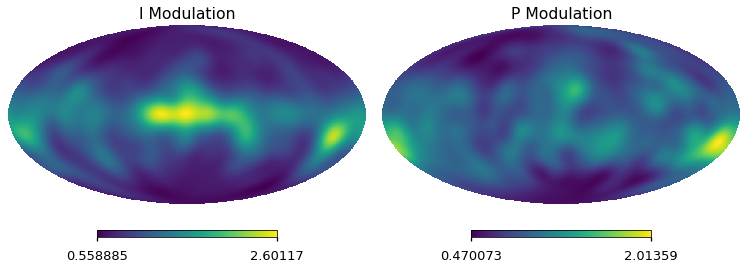
\includegraphics[width=2\columnwidth]{figures/mod_dust.png}\\
      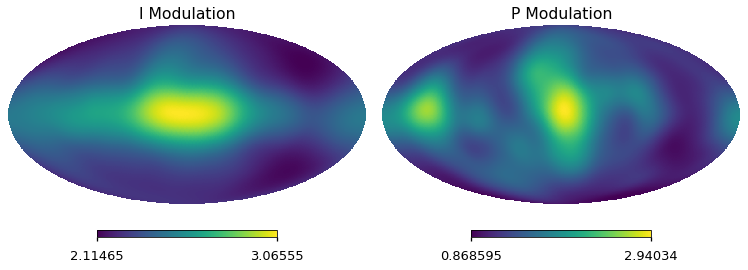
\includegraphics[width=2\columnwidth]{figures/mod_synch.png}\\
     \caption{Modulation maps $m_i$ and $m_p$ for (top) dust and  (bottom) synchrotron. }
     \label{fig:modulation_maps}
 \end{figure*}
 
The $\ell_1$, $\ell_2$, and $\ell_*$ values used to construct the modulation maps are presented in Table~\ref{tab:smallscale_par}. The values of $\ell_1$ and $\ell_*$ are driven both by the angular resolution and the signal-to-noise ratio of the template maps. We employ $\ell_1=100$ and $\ell_*=80$ for dust and $\ell_1=38$ and $\ell_*=36$ for synchrotron. The $\ell_2$ parameter is chosen to be high enough that dust and synchrotron emission are relatively unconstrained by current full-sky data. We adopt  $\ell_2=2000$ for dust and $\ell_2 = 400$ for synchrotron. The modulation maps are illustrated in Figure~\ref{fig:modulation_maps}.

%Given that the intensity template has been estimated in a different way to the Q and U templates, we employ two different multipole scale cut-offs: $\ell=400$ and $100$, respectively. This further prevents the mixing of scales due to variable resolutions.

%\giuse{increasing at $\ell>40$ in the K-band spectra estimated by masking 80\% of the sky.  Therefore, we  adopt $\ell = 36$ as  cut-off multipole scale  for synchrotron.}

The final maps are obtained from 
\begin{equation} \label{eq:filter}
    a_{\ell m }^{X, out}=  a_{\ell m }^{x, \mathcal{T}} \left(1-\sigma_\ell\right)^{0.2} + a_{\ell m }^{x, ss} \sigma_\ell
    ~~~, 
\end{equation}
where $a_{\ell m }^{X, \mathcal{T}}$ are the coefficients of the large-scale templates, with $X$ any of $t$, $e$, and $b$, and $a_{\ell m }^{X, ss}$ is derived from the synthesized small-scale fluctuation maps. The filter $\sigma_\ell$ is given by
%Thus, the power spectra are described by
%\begin{equation} \label{eq:filter}
%    C_\ell^{xy} = C_\ell^{xy, \mathcal{T}}\left(1-\sigma_\ell\right)^{0.4} + C_\ell^{xy, ss} \sigma_\ell 
%\end{equation}
%where $C_\ell^{xy, \mathcal{T}}$ are the power spectra of the data-driven templates (Section~\ref{sec:templates}), $xy$ is any of $tt$, $te$, $ee$, and $bb$. The filter $\sigma_\ell$ is given by

\begin{equation}
\sigma_\ell  = \left[1+  e^{ -c_1 (\ell/ \ell_1  -c_2 )}\right]^{-1}  
~~~,
\end{equation}
where the parameters $c_1$ and $c_2$ govern the width of the filter in multipoles. We adopt $c_1=40$ and $c_2=0.9$ throughout this work. The exponent of $0.2$ on the $\left(1-\sigma_\ell\right)$ term in Equation~\ref{eq:filter} is chosen empirically to smooth the transition between our data-driven templates and the generated small scales. We found that this choice minimizes artifacts at $\ell \simeq \ell_1$ in power spectra computed over large sky areas while maintaining the correct asymptotic behavior.

Since the generation of the small scales depends only upon a fixed input power spectrum, we can generate a different map realization on the fly each time a sky is simulated. Thus, the methodology presented here enables generation of an ensemble of sky realizations having the same well-measured large scales but stochastic realizations of the poorly-measured small scales. Further, the small-scale fluctuations can be generated at arbitrarily small scales set only by the resolution of the map since all power spectra can be extended indefinitely in $\ell$. In practice, small scales are generated up to a \af{maximum linearly independent} $\ell_{\rm max} = 3N_{\rm side}-1$.

We do not intend for the above procedure to be useful for the inner Galactic plane, which has been imaged at high signal-to-noise ratio at relatively small scales. We thus do not apply the small-scale amplitude extrapolation to the $3\%$ of the sky in the Galactic plane as defined by the Planck \texttt{GAL097} mask\footnote{\texttt{HFI\_Mask\_GalPlane-apo2\_2048\_R2.00.fits}}, where we instead use the observed templates as-is at all scales. To ensure a smooth transition between the template used in this region and synthesized small scales employed over the rest of the map, we apodize the mask with a $5^\circ$ Gaussian taper. This reflects our expectation that our procedure is most useful for making physically motivated synthetic realizations of diffuse Galactic emission at high Galactic latitudes rather than in the Galactic plane.

% BH: To go through and ensure all is captured in the text above
%We first compute the $tt$, $ee$, and $bb$ power spectra from the dust template $i$, $q$, and $u$ maps and fit each with a power law $A\ell^{\gamma}$ in different multipole ranges depending on the native resolution of the map. Given that the intensity template has been estimated in a different way to the Q and U templates, we employ two different multipole scale cut-offs: $\ell=400$ and $100$, respectively. This further prevents the mixing of scales due to variable resolutions. Specifically, we employ $100 < \ell < 400$ for $tt$ and $30 < \ell < 110$ for $ee$ and $bb$. The spectral indices estimated from the fit are $\gamma = -1.29$, $-0.33$, and $-0.40$ for $tt$, $ee$, and $bb$, respectively.Adopting these values of $\gamma$ directly would lead to the $ee$ and $bb$ power exceeding $tt$ for large enough $\ell$ given the steeper index of the latter. {\bf Some words on why this is ok in principle but gives problems with polarization fraction in practice} We prevent this by adopting a common spectral index $\gamma = -1.29$ to extrapolate all three spectra to higher $\ell$. This choice is further motivated by the fact that the dust intensity template is provided at a higher resolution than the polarization ones, allowing to observe the dust specifics at higher detail with respect to the polarization data being more affected by noise and systematics. Although we are assuming that small scale polarized dust emission to be the same spectral index as the intensity one, this  is something that is physically intuitive and expected   from magneto-hydro dynamic simulations \citep[][]{Kim:2019}. We then generate $iqu$ maps encoding only small scales generated from the fit power law spectra and ranging from the pivot $\ell$-scale up to the multipole related to the desired pixel resolution scale of the dust map we want to simulate.  
%Since we want the small scales to be modulated by the amplitude of the dust emission at large scales, we apply two different modulations for the $i$ and for the $qu$ maps as they are convolved with different beam resolutions. We adopt  the $i$  map   smoothed at 5 deg as a template for both modulation maps.  We then identify a region encoding  low and intermediate Galactic latitudes by masking  all the pixels in the smoothed $i$ map  whose  value is $>4.5 \log ( \mu K )$.  The  intensity modulation is then constructed by performing two different normalization in the regions defined outside and inside  the mask. We use the \emph{MinMax} rescaling ranging   between $1$ and $2$ for the low-intermediate latitudes and between $0.1$ and $1$ for the high latitudes. For the polarization modulation map, we rescale similarly outside the mask between $0.1$ and $1$ but we saturate to   $1$  all the pixels  inside the low latitude region. Once the small scale maps are modulated, they are then co-added to the  low-pass filtered  $iqu$ maps (given the $\ell$-pivot scale) that encode  large scales only. Finally, the $iqu$ maps are transformed   back to the real $IQU$ maps  to perform the validation steps required to assess the quality of the maps. 

\subsubsection{Dust Amplitude}\label{sec:dustamplitude}
The Planck~2015 component separation results in total intensity remain state of the art despite updates in polarization in the 2018 data release \citep{planck2016-l04}. Previous PySM models, e.g., \texttt{d0} and \texttt{d1}, employed the dust templates from the \texttt{Commander} component separation analysis \citep{planck2014-a11}. However, the model fitting employed in \citet{planck2014-a11} did not differentiate between Galactic dust emission and the Cosmic Infrared Background (CIB), and so the component separated dust maps retain CIB signal that should not be included in simulations of Galactic emission (see Section~\ref{sec:CIBcontamination} for a detailed discussion). To address this issue, we instead use dust templates from analyses that separated Galactic dust emission from the CIB using the Generalized Needlet Internal Linear Combination (GNILC) algorithm \citep{Remazeilles:2011}. 

In total intensity we employ the Planck GNILC 2015 component separated map at $353$\,GHz \citep{planck2016-XLVIII}\footnote{\texttt{COM\_CompMap\_Dust-GNILC-F353\_2048\_R2.00.fits}}. This map has variable angular resolution, ranging from $21.8\arcmin$ up to $5\arcmin$ depending on the sky regions, which complicates its use in our analysis. Therefore, we reprocess the map as follows to a spatially uniform resolution of 21.8\arcmin. To do so, we first note that the map was synthesized from ten needlet maps of different, but spatially-uniform, resolution \citep[][Figure~A.2]{planck2016-l04}. We produce a map of uniform resolution by retaining only the first six needlet maps, which probe the dust intensity from the largest scales down to $21.8\arcmin$. This yields an $N_{\rm side} = 2048$ that reproduces the Planck GNILC 2015 dust intensity template at all scales $\geq 21.8$\arcmin. Finally, we subtract the CIB monopole of $0.13\, \text{MJy}\,\text{sr}^{-1}$ present in the map \citep[][Section~2.2]{planck2016-l11B}.

For the dust $Q$ and $U$ maps we employ the dust maps\footnote{\texttt{COM\_CompMap\_IQU-thermaldust-gnilc-varres\_2048\_R3.00.fits}} produced by the GNILC component separation from the Planck Public Release 3 \citep{planck2016-l04,planck2016-l11B}. While these maps have variable angular resolution, the resolution varies over the sky much more smoothly than in the $I$ map. Given this, and that we wish to retain as much polarization information in our analysis as possible, we employ these variable resolution maps as-is. Their resolution ranges from $21.8\arcmin$ in the Galactic plane to $80\arcmin$ at high Galactic latitudes. The maps are pixellated at $N_{\rm side} = 2048$. 

To produce dust emission templates at a monochromatic frequency of 353\,GHz, we divide each of the $I$, $Q$, and $U$ maps by a factor of 1.098 to correct for the Planck bandpass \citep[][Table~2]{planck2016-l11A}.

\subsubsection{Synchrotron Amplitude}
Deriving a full-sky template for synchrotron emission in total intensity is challenging both for the paucity of low frequency surveys with full sky coverage and the difficulty in disentangling synchrotron emission from free-free emission and AME at frequencies above $\sim$10\,GHz. We follow \citet{Thorne:2017} in basing our template on the Haslam 408\,MHz survey with reprocessing \citep{Remazeilles:2015}. We rescale the 408\,MHz map of \cite{Remazeilles:2015} to 23\,GHz assuming a sky-constant power law $I_\nu \propto \nu^{-3.1}$. Finally, we smooth the resulting map to a resolution of $2^\circ$.

Constructing a synchrotron template in polarization is somewhat easier than total intensity because both free-free emission and AME have very low levels of polarization. Thus, we employ the WMAP K-band (23\,GHz) $Q$ and $U$ maps directly as our templates. As with the $I$ map, we smooth the $Q$ and $U$ templates to a resolution of $2^\circ$.

% BH: Did we do anything about bandpasses?

\subsection{Small Scale Fluctuations in Spectral Parameters} \label{sec:spec_params}

\subsubsection{Methods Overview}
\begin{table}
    \centering
    \begin{tabular}{lcc}
    \toprule 
   &   $ \ell_1   $    &$\alpha$  \\
   \midrule  
   $\beta_d$ & 400 & 0.04 \\ 
   $T_d$  &  400  & -0.47\\
    \midrule 
    $\beta_s$ & 38 & -0.61\\
    $c_s$ & 38 &  -0.61  \\ 
   \bottomrule
    \end{tabular}
    \caption{Spectral indices adopted for synthesizing  small scales in the spectral parameters of dust and synchrotron models. }
    \label{tab:smallscale_specpar}
\end{table}

Just as a map of Galactic emission at a single frequency is expected to have fluctuations at smaller angular scales than have been measured, maps of parameters governing its frequency dependence should also have small-scale fluctuations. We therefore introduce small scale fluctuations to our spectral parameter template maps in a way analogous to the amplitude template maps. This more realistically captures the complexity of small-scale Galactic emission.

As there is no sense of polarization in the spectral parameter maps, we do not work within the polarization fraction tensor framework but rather with standard power spectra. Given a template map $\mathcal{T}$ of some spectral parameter $\beta$, we first fit the power spectrum of $\mathcal{T}$ with a power law $C_\ell \propto \ell^\alpha$ over a range of scales where it is well measured, up to some multipole $\ell_1$. We then generate a map of small scale fluctuations using the power law fit. We multiply the resulting map by a modulation map in analogy with the amplitude modulations described in Section~\ref{sec:dustamplitude}. Finally, we combine the template map with the synthesized small scales using the filter function in Equation~\ref{eq:filter}.

The application of this procedure to the dust and synchrotron spectral parameters is described in the following sections. The adopted fit parameters for each spectral parameter are listed in Table~\ref{tab:smallscale_specpar}.

\subsubsection{Dust Spectral Parameters}\label{subsec:dust_spec_params}
As described in Section~\ref{subsubsec:dust_model}, the dust emission in all models developed here is governed by the spectral parameters $\beta_d$ and $T_d$. For the $\beta_d$ and $T_d$ template maps, we employ the $\beta_d$ and $T_d$ maps\footnote{\texttt{COM\_CompMap\_Dust-GNILC-Model-Spectral-Index\_2048\_R2.00.fits}, \texttt{COM\_CompMap\_Dust-GNILC-Model-Temperature\_2048\_R2.00.fits}} derived from 2015 Planck GNILC component separation analysis \citep{planck2016-XLVIII}. These maps benefit from lower CIB residuals than the \texttt{Commander} $\beta_d$ and $T_d$ as the methodology employed both spatial and spectral information to disentangle the CIB contribution to the total emission.
%However, the estimate of $\beta_d$ and $T_d$ is highly degenerate making the maps at small angular scales ($<21.8^\prime$) are contaminated by artifacts due to noise and calibration errors. 

We fit the power spectra of the $\beta_d$ and $T_d$ template maps over the multipole ranges $200 < \ell < 400$ and $100 < \ell < 400$, respectively. We find that $\alpha_{\beta_d}= 0.04$ and $\alpha_{T_d} = -0.47$ over this range, both flatter than the $\alpha_{tt} = -0.80$ found for the dust amplitude. The adopted pivot multipole $\ell_1$ is larger than that used for dust amplitudes (see Table~\ref{tab:smallscale_par}) since the template maps employed here are derived from intensity-only data rather than a combination of total and polarized intensity. Thus, they remain signal-dominated at $\sim$4 times smaller angular scales.

%The chosen cut-off multipole for $\beta_d$ and $T_d$ is the same as the one adopted for the intensity amplitude template, i.e., $\ell=400 $.

We construct the modulation map from the GNILC $I$ map smoothed to a resolution of $5^\circ$. We apply a linear renormalization such that the (now dimensionless) pixel values in the map range from 0.1 to 2. %BH The text below makes me think that pixels in the I map above and below a certain threshold were ignored in this process rather than taking the literal min and max values of the map

%\giuse{ Also in this case, we   employ a modulation map for the $\beta_d$ and $T_d$ synthetic small scales.   The modulation template is derived from $I$ GNILC amplitude map, smoothed  at 5 deg and \emph{min-max} normalized   from $0.1$ and $2$. The latter step is needed as we expect the modulation map to be dimensionless and  the extreme values have been  empirically identified as the best choice to preserve the range of variation observed in   $\beta_d$ and $T_d$ at both low and intermediate Galactic latitudes. } 

% BH: This is potentially important, but probably belongs in the validation section
%However,  we do not expect small scales generated with the spectral parameter maps  to dominate when rescaling maps at frequencies other than the reference one (353 GHz). \giuse{This is mainly granted by the fact that amplitude small scales are few orders of magnitude larger than the ones injected in the  spectral parameter, in the whole range of reliability of the PySM models, e.g. 10-1000 GHz.}
 
\subsubsection{Synchrotron Spectral Parameters}\label{sec:beta_s}
As described in Section~\ref{subsubsec:synch_model}, the synchrotron emission in all models developed here is governed by the spectral parameters $\beta_s$ and $c_s$. To build the large scale template for the spatial variation of the synchrotron spectral index $\beta_s$, we begin with the full-sky $\beta_s$ map obtained by combining the Haslam map in total intensity at 408\,MHz \citep{Remazeilles:2015} and WMAP K-band data \citep{Miville-Deschenes:2008}. The map has an angular resolution of about $7^{\circ}$ and was employed by previous PySM synchrotron models \citep{Thorne:2017}.

Incorporating newer constraints on synchrotron emission at 2.3\,GHz from S-PASS, \citet{Krachmalnicoff:2018} determined that this $\beta_s$ map underestimates the true level of spatial variations in $\beta_s$ across the Southern Galactic Hemisphere. Thus, we follow \citet{Krachmalnicoff:2018} and rescale the $\beta_s$ map by first subtracting its mean value, multiplying the resulting map by a factor of $1.572$, and then adding back the mean value.

We next fit a power-law to the power spectrum of this new template map over the multipole range $2<\ell<38$, finding $\alpha_{\beta_s}=-0.61$ then construct a map from this power spectrum extrapolated to high multipoles. We next construct a modulation map by taking the Haslam 408\,GHz $I$ map, smoothing to $5^\circ$ resolution, then renormalizing the map through a linear transformation such that the (dimensionless) pixel values range from 0.1--2. As with the dust spectral parameter maps (see Section~\ref{subsec:dust_spec_params}), we combine this high-$\ell$ map with the low-$\ell$ template following the filter function of Equation~\ref{eq:filter}.
 
For the synchrotron curvature parameter $c_s$, there are no readily available template maps. The existing \texttt{s3} model implements curvature as a sky-constant $c_s = -0.052$, consistent with the measurements from ARCADE \citep[$c_s=-0.052 \pm 0.005$,][]{Kogut:2012}. As an attempt to model a reasonable range of spatial variability, we assume that fluctuations in the value of $c_s$ follow the synchrotron intensity at large angular scales. Specifically, we start from the Haslam map 408\,MHz $I$ map smoothed to a resolution of $5 \deg$, which we then rescale with a linear transformation such that the minimum and maximum pixel values are  $-0.0517$ and $0.0054$, respectively, corresponding to the range of $c_s$ measurements from ARCADE \citep{Kogut:2012}. The resulting $c_s$ map has a mean and standard deviation of $-0.0517$ and $0.0054$, respectively. 

% BH: If this was done, it needs to be described quantitatively with reference to the relevant equations
%Finally, both the $\beta_s$ and the $c_s$ templates are low pass filtered with $\ell=36$ to minimize artifacts from noise and the large beamsize.

To extend our $c_s$ map to angular scales $\ell > 36$, we first generate a map of Gaussian random fluctuations with the same power law index as the $\beta_s$ map, i.e., $\alpha _{c_s}=\alpha _{\beta_s} = -0.61$. We modulate the resulting map with the same modulation map as used for $\beta_s$ and combine this high-$\ell$ map with the low-$\ell$ template following the filter function of Equation~\ref{eq:filter}.
%Small  scales at multipoles $\ell>36$  are therefore  included   assuming them to follow  the same power law as  the $\beta_s$ ones,  i.e. $\alpha _{c_s}=\alpha _{\beta_s} = -0.61$, and that are  modulated with the exact same modulation map as the one we  adopted for $\beta_s$.

\subsection{Summary of New Dust and Synchrotron Models}

% \begin{figure*}
%     \centering
%     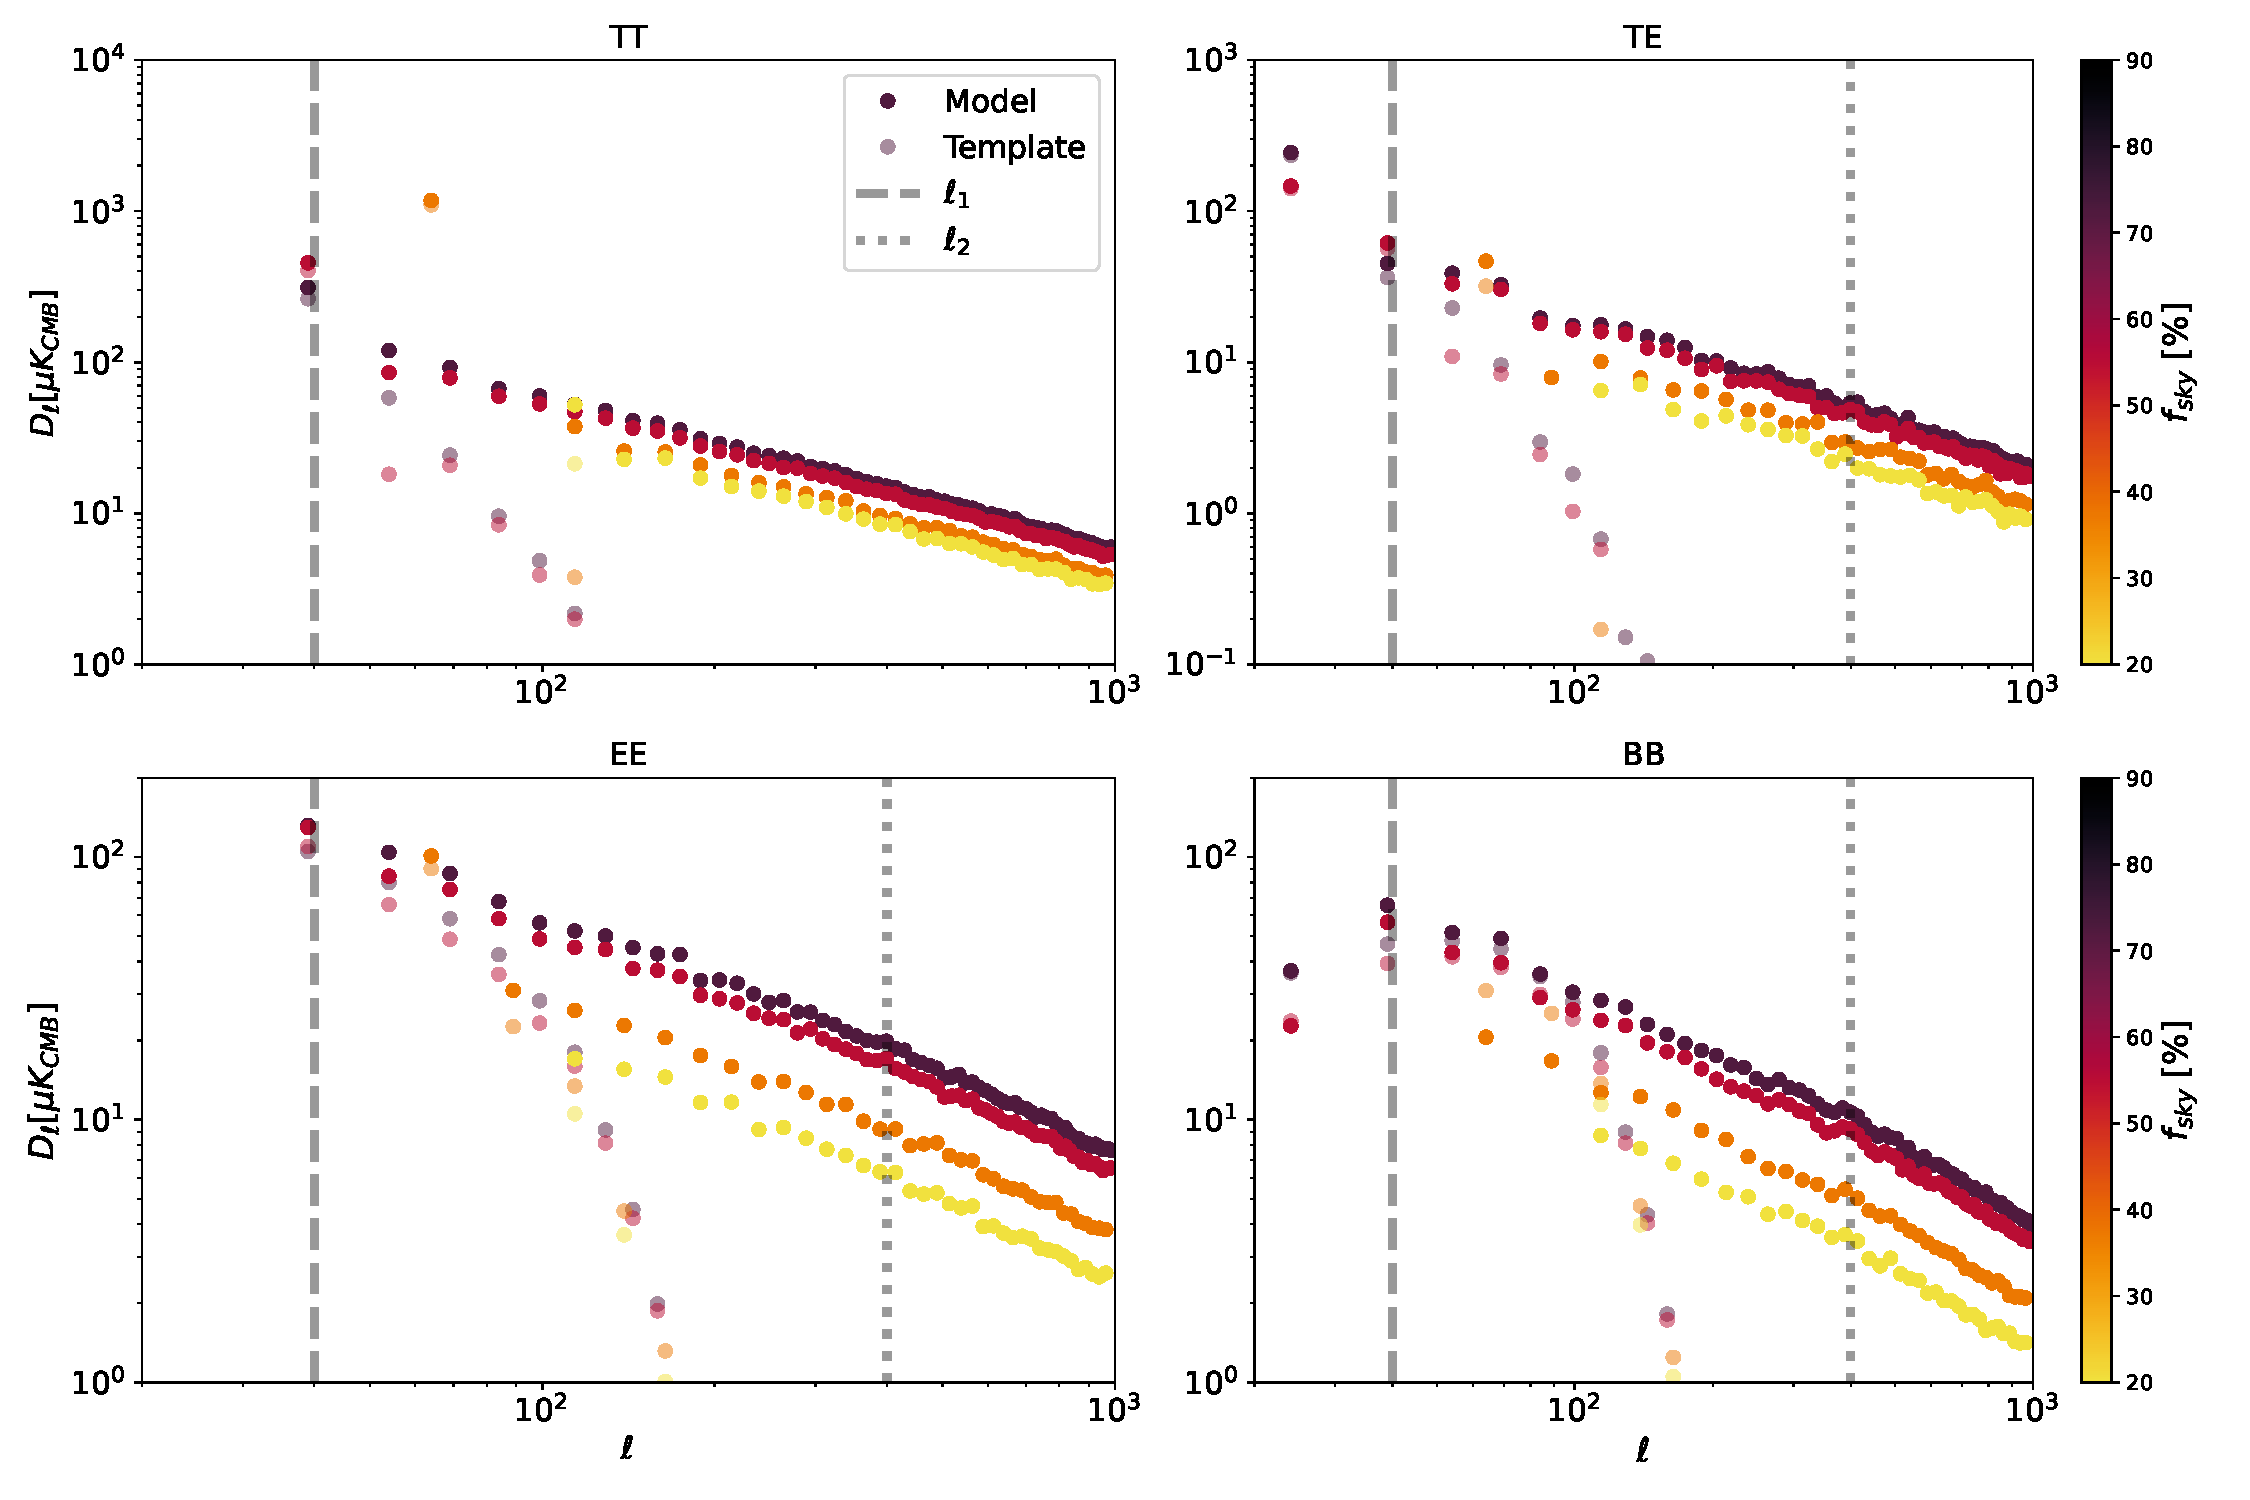
\includegraphics[width=2.\columnwidth]{figures/synch_valspectra.pdf}
%     \caption{This figure compares the power spectra of the \texttt{s4} model (dark circles) and the input HASLAM/WMAP K-band  map (light circles) when computed on the \texttt{GAL090}, \texttt{GAL070}, \texttt{GAL040}, and \texttt{GAL020} Galactic masks.}
%     \label{fig:spectra_by_field}
% \end{figure*}
The new dust and synchrotron models implemented here all improve on previous models through new data-driven templates and use of the polarization fraction tensor framework to model small-scale fluctuations. Multiple models each of dust and synchrotron are provided to explore a range of astrophysical complexity allowed by current constraints. In brief, the d9 and s5 models use the new data-driven templates and include $I$, $Q$, and $U$ fluctuations up to the largest $\ell$ values simulated, but these models have sky-constant spectral parameters and thus no frequency decorrelation (see Section~\ref{subsec:decorrelation} for discussion). In contrast, d10 and s5 employ data-driven maps of spectral parameters to which small-scale fluctuations are added, inducing frequency decorrelation. The s7 synchrotron model provides an extra spectral parameter---curvature of the frequency spectrum---and thus additional complexity. The d11 and s6 models allow many realizations of d10 and s5, respectively, to be generated in which the large scales are fixed to the data-driven templates and the small scales have the same statistical properties but differing spatial morphologies. Extensive model comparisons are made in Section~\ref{sec:validation}.

\section{Other Models Implemented} \label{sec:other_models}

\subsection{Dust Layer Model} \label{sec:layers}
Evidence for variation of Galactic foreground emission laws as a function of frequency across the sky implies that emission laws must also vary along the line of sight \citep{Martinez-Solaeche:2018}. As a consequence, even if dust emission can be described locally by a modified blackbody (Equation~\ref{eq:dust-emission-law}), a superposition of emission regions (i.e., an integral along the line of sight) is not a modified blackbody. In addition, if along the line of sight different line elements emit polarized radiation with different polarization angles, the frequency scaling can vary between $I$, $Q$ and $U$ \citep{Tassis:2015}. Evidence for this ``line-of-sight frequency decorrelation'' has been found in Planck data \citep{Pelgrims:2021}.

To model the complexity of multiple layers of dust along the line of sight, we base our  PySM~3 implementation \texttt{d12} on the approach of \cite{Martinez-Solaeche:2018} in the PSM software\footnote{See version 2.3.3 \url{https://apc.u-paris.fr/~delabrou/PSM/psm.html}.}. 

The PSM has been run to produce six maps of dust emission $S_{\nu_0}^k(\theta)$ at $\nu_0 = 353$ GHz (intensity and polarization, for a total of 18 HEALPix maps at nside=2048), and six maps of dust spectral index $\beta_d^k(\theta)$ and dust temperature $T_d^k(\theta)$ at nside=2048, following the approach described in \cite{Martinez-Solaeche:2018}, to form six different layers.

%The PSM has been run to produce six maps of dust emission at 353~GHz (intensity and polarization, for a total of 18 HEALPix maps at {\tt nside=2048}), and six maps of dust spectral index $\beta_d$ and dust temperature $T_d$, also at {\tt nside=2048}, following the approach described in \cite{Martinez-Solaeche:2018}. 

The PySM software uses these maps as inputs, and generates the dust Stokes parameters maps as:
\begin{equation}
    S_\nu(\theta) = \sum_{k=1}^6 S^{(k)}_{\nu_0}(\theta)
    \left( \frac{\nu}{\nu_0} \right)^{\beta^{(k)}_d(\theta)}
    \frac{B_\nu(T^{(k)}_d(\theta))}{B_{\nu_0}(T^{(k)}_d(\theta))},
\end{equation}
where $S_\nu(\theta)$ stands for any of the three Stokes parameters of interest, $I$, $Q$ and $U$, at frequency $\nu$ at sky location $\theta$, and superscripts ${(k)}$ indicate the layer, from one to six.

In the implementation used here, the 353~GHz templates for the six emission layers are slightly different from those of \cite{Martinez-Solaeche:2018} as we construct them from more recent Planck data products. Large scale polarized emission maps are the GNILC maps obtained in \cite{planck2016-l04} using the method developed by \cite{Remazeilles:2011}. These are complemented by small scale realizations with scale dependence matching the $I$, $E$ and $B$ dust spectra measured in \cite{planck2016-l11A}, modulated by the large scale local intensity and polarized intensity level. Specifically, for each layer $k$, and for each of $T$, $E$ and $B$, we model the final emission in harmonic space as:
\begin{equation}
    S^{(k)}_{\nu_0} = X^{(k)}_{\nu_0} h_\ell^{1/2} + Y^{(k)}_{\nu_0} (1-h_\ell)^{1/2},
\end{equation}
where $X^{(k)}_{\nu_0}$ is the observed emission deconvolved from the instrumental beam, $Y^{(k)}_{\nu_0}$ is a randomly generated set of harmonic coefficients with harmonic spectrum following Planck constraints \citep{planck2016-l11A}, and $h_\ell$ is a window defining the transition between the two regimes. For intensity, $h_\ell$ corresponds to a 5\arcmin\ beam window function, while for polarization, we use a 150\arcmin\ beam for the three nearest layers (which dominate at high Galactic latitude) and a 120\arcmin\ beam for the three farthest layers (which dominate near and in the Galactic plane).

The construction of these maps does result in some filtering out of the real small scale power in intensity and polarization, which is replaced by random fluctuations. Thus we expect departures from the non-Gaussian and non-stationary properties of real dust emission at these scales.

In this model, maps of spectral parameters ($\beta_d$ and $T_d$) are randomly generated for each layer as described in \cite{Martinez-Solaeche:2018}. As a consequence, they are not constrained to match the observed temperature and spectral index maps. While their statistics (e.g., amplitude, correlation between $\beta_d$ and $T_d$) are compatible with those of real data, they provide a different realization, which results in increased differences between the real sky and the model at frequencies increasingly far from the reference frequency, $\nu_0 = 353$~GHz.

\subsection{CO Models} \label{subsec:co_models}
Galactic CO line emission is strong enough that the $J = 1\rightarrow0$, $J = 2\rightarrow1$, $J = 3\rightarrow2$ transitions have been detected even in the broad photometric Planck bands \citep{planck2013-p03a, planck2014-a12}. Since CO emission can be polarized \citep{Goldreich:1981}, it may be a relevant foreground for CMB polarization analyses \citep{Puglisi:2017}. In this section, we describe the implementation of three CO models into the PySM~3 framework.

All CO models implemented here are based on the CO $J = 1\rightarrow0$, $J = 2\rightarrow1$, $J = 3\rightarrow2$ \texttt{Type-1} intensity maps\footnote{\url{HFI_CompMap_CO-Type1_2048_R2.00.fits}} derived by \citet{planck2013-p03a} from Planck data. The CO maps are obtained exploiting the mismatches in the detector bandpasses to recover the CO from the CMB and the other Galactic foregrounds using the Modified Internal Linear Combination Algorithm (\texttt{MILCA}). The templates produced from this analysis are preferred to direct measurements from existing spectroscopic surveys \citep[e.g.,][]{Dame:2001} because they are not limited to low Galactic latitudes and have a uniform angular resolution over the sky.

\citet{planck2013-p03a} also produced \texttt{Type-2} templates based on a multi-frequency analysis. However, this method is more prone to modeling errors in separating the Galactic dust emission from the CO emission, and so we prefer the \texttt{Type-1} templates for our purposes.

The \texttt{Type-1} CO templates have a native resolution of 10\arcmin. We convolve each of the $J = 1\rightarrow0$, $J = 2\rightarrow1$, and $J = 3\rightarrow2$ maps with a 1$^\circ$ Gaussian beam to reduce noise contamination especially at intermediate and high Galactic latitudes at the possible expense of introducing residual emission from extended Galactic and extra-galactic sources. Finally, the templates are downgraded to a coarser pixellization of \texttt{nside=512}. These templates are the foundation on which the CO models are built.

The first CO model {\bf\texttt{co1}} adopts the $J = 1\rightarrow0,$  $J = 2\rightarrow1$ and $J = 3\rightarrow2$ templates as-is and assumes no polarization. 

The second CO model {\bf\texttt{co2}} introduces a simple implementation of polarization. The $I$ maps of the three transitions used in  {\bf\texttt{co1}} are converted to $P$ maps using a sky-constant, user-defined polarization fraction $p$, where the default is $p = 0.1$\%. The $Q$ and $U$ maps are made from the $P$ maps using the polarization angle of the thermal dust emission as determined by a component separation analysis with Commander \citep{planck2014-a12}.

Finally, the third CO model {\bf\texttt{co3}} not only accounts for the polarized emission as in {\bf\texttt{co2}} but also includes small-scale emission from high-Galactic latitude clouds. We perform a dedicated simulation with the {\bf\texttt{LogSpiral}} model from \citet{Puglisi:2017}, which provided the best fit to Planck data, to produce maps of the contribution to the total and polarized CO intensity at sub-degree scales from molecular clouds at high Galactic latitudes. The $I$, $Q$, and $U$ maps generated by the simulation are then added to the $I$, $Q$, and $U$ maps of {\bf\texttt{co2}} to produce the final {\bf\texttt{co3}} model.
 
\section{Validation and Characterization of Models} \label{sec:validation}

In this section, we validate the foreground models developed in Section~\ref{sec:small_scales}.
%
%\giuse{We firstly show a comparison in Section~\ref{subsec:maps} at the map level of the new models, to visually appreciate the differences between with the templates and the previous PySM models.} 
In Section~\ref{subsec:maps}, we show map comparisons to visually appreciate the differences between the various PySM models and real-sky observations.
%
% In Section~\ref{sec:dust_validation} we demonstrate that the two-point statistics of the stochastic small scales are properly modulated for different regions of sky defined by Galactic masks of varying size. We also assess the properties of our dust model in the small patch of sky observed by the BICEP / Keck telescopes and the South Pole Telescope.  
%
%\sg{In Section~\ref{sec:sync_validation} we compare the power spectra of different synchrotron models with BeyondPlanck synchrotron map for temperature, and LFI 30 GHz for polarization. We find a reasonable agreement between the data and our models for different fraction of the Galactic synchrotron signal masked.} 
\sg{In Section \ref{sec:PS-validation} we compare power spectra for the PySM dust and synchrotron models with observations. We demonstrate that the two-point statistics of the stochastic small scales are properly modulated for different regions of sky defined by Galactic masks of varying size. Section~\ref{sec:dust_validation} shows the comparison of PySM dust models with Planck NPIPE maps at 353 GHz. 
While in Section~\ref{sec:sync_validation}, we compare the PySM synchrotron models with the synchrotron map from the BeyondPlanck analysis for intensity, and with the Planck Revisited reprocessed maps for polarization. We also show dust and synchrotron model spectra validation in the sky patch observed by the BICEP/Keck telescopes in Section~\ref{sec:BK_validation}.}
%
\giuse{/bf describe also section on decorrelation}. In Section~\ref{sec:nongaussianity}, we assess the level of non-Gaussianity introduced by the log polarization tensor formalism, and compare this to the case of a purely Gaussian small scale model which has been modulated by a Galactic template. 


\subsection{Maps}\label{subsec:maps}

PySM models are based on noisy observations of Galactic foreground amplitude maps, complemented in some cases by randomly generated small-scale features (sec.~\ref{sec:small_scales} and \ref{sec:layers}). Maps of frequency scaling parameters also comprise randomly generated fluctuations, the generation of which is different for the various models. 

%It is important to check to which extent model maps match with observations in the frequency range of interest. 
In this first step of validation of the PySM foreground models, we compare maps generated using the PySM and actual observations in the frequency range of interest for the different foreground models considered here. %\textcolor{red}{[What frequencies do we want to cover? I suggest at least 23~GHz--353~GHz, but this does not fully cover the frequency range of CMB-S4 and LiteBIRD]}
% Jacques
Specifically, we compare, at the map level, observations of the Planck third data release PR3 \cite{planck2016-l03} and PySM dust models \texttt{d1} (which was widely used as a reference in previous versions of the PySM, and is described in \cite{Thorne:2017}), {\tt d9} (which is similar to \texttt{d1}, but uses different input templates and includes small scale fluctuations of template maps and spectral parameters, as described in sec.~\ref{sec:small_scales}), and {\tt d12}, which is conceptually quite different from the other two.

%In this comparison, we want to compare the PySM models that don't include randomly generated small-scales (d1 and d12) \textcolor{red}{[JD: this is not correct, d12 at least contains randomly generated small scales]} with models that include them (d9). 
%As \texttt{d9} has random fluctuations generated as described in section \ref{sec:small_scales}, we expect that we do not recover as well the small scales in data as for the d12 model \ref{sec:layers}. %discuss what we expect for d1
We study how the modeled intensity $I$ and polarized intensity $P = \sqrt{U^2 + Q^2}$ compare to the observations on selected $16.7^\circ \times 16.7^\circ$ patches of the sky, at 353~GHz. We focus on two patches, one close to the Galactic plane ($[l,b] =[180^\circ,-10^\circ]$) and the second centered on the Bicep/Keck field ($[l,b] =[318^\circ,-61^\circ]$).

We integrate the dust models in the Planck passband (\cite{planck2013-p03d}).\footnote{\url{http://pla.esac.esa.int/pla/aio/product-action?MAP.MAP_ID=HFI_RIMO_R3.00.fits}} For the comparison of intensity maps, we subtract a Wiener-filtered CMB temperature anisotropies map from SMICA and also adjust (setting to zero) the zero level of the PR3 data and the simulated maps over a small region of very low dust emission, totaling a sky fraction of 2.5\%.
%to that of the simulated map over regions of faint dust intensity on the sky.
This readjustment is slightly different for the three dust models and the data considered (i.e., the zero level is not exactly the same in all the maps). 
%We compute the mean of the intensity in the regions considered for the three dust models and data and then subtract this quantity from the dust intensity of each model and data.
The mask used to adjust the zero levels is shown in Figure~\ref{fig:mask_zero_lvl_int}. 
These corrections are not required for comparing polarization data. 
%PR3: 13.97uKcmb
%d9: 14.46uKcmb
%d11: 14.59uKcmb
%d12: 6.41uKcmb
%note: JD - there is considerable uncertainty on the zero level of the maps (if I got my calculations right, the CIB monopole at 353GHz is of the order of 300uKcmb, and is not known with 5% accuracy -- the difference between models based on FIRAS is more like 10-20%)


\begin{figure}[ht!]
    \centering
    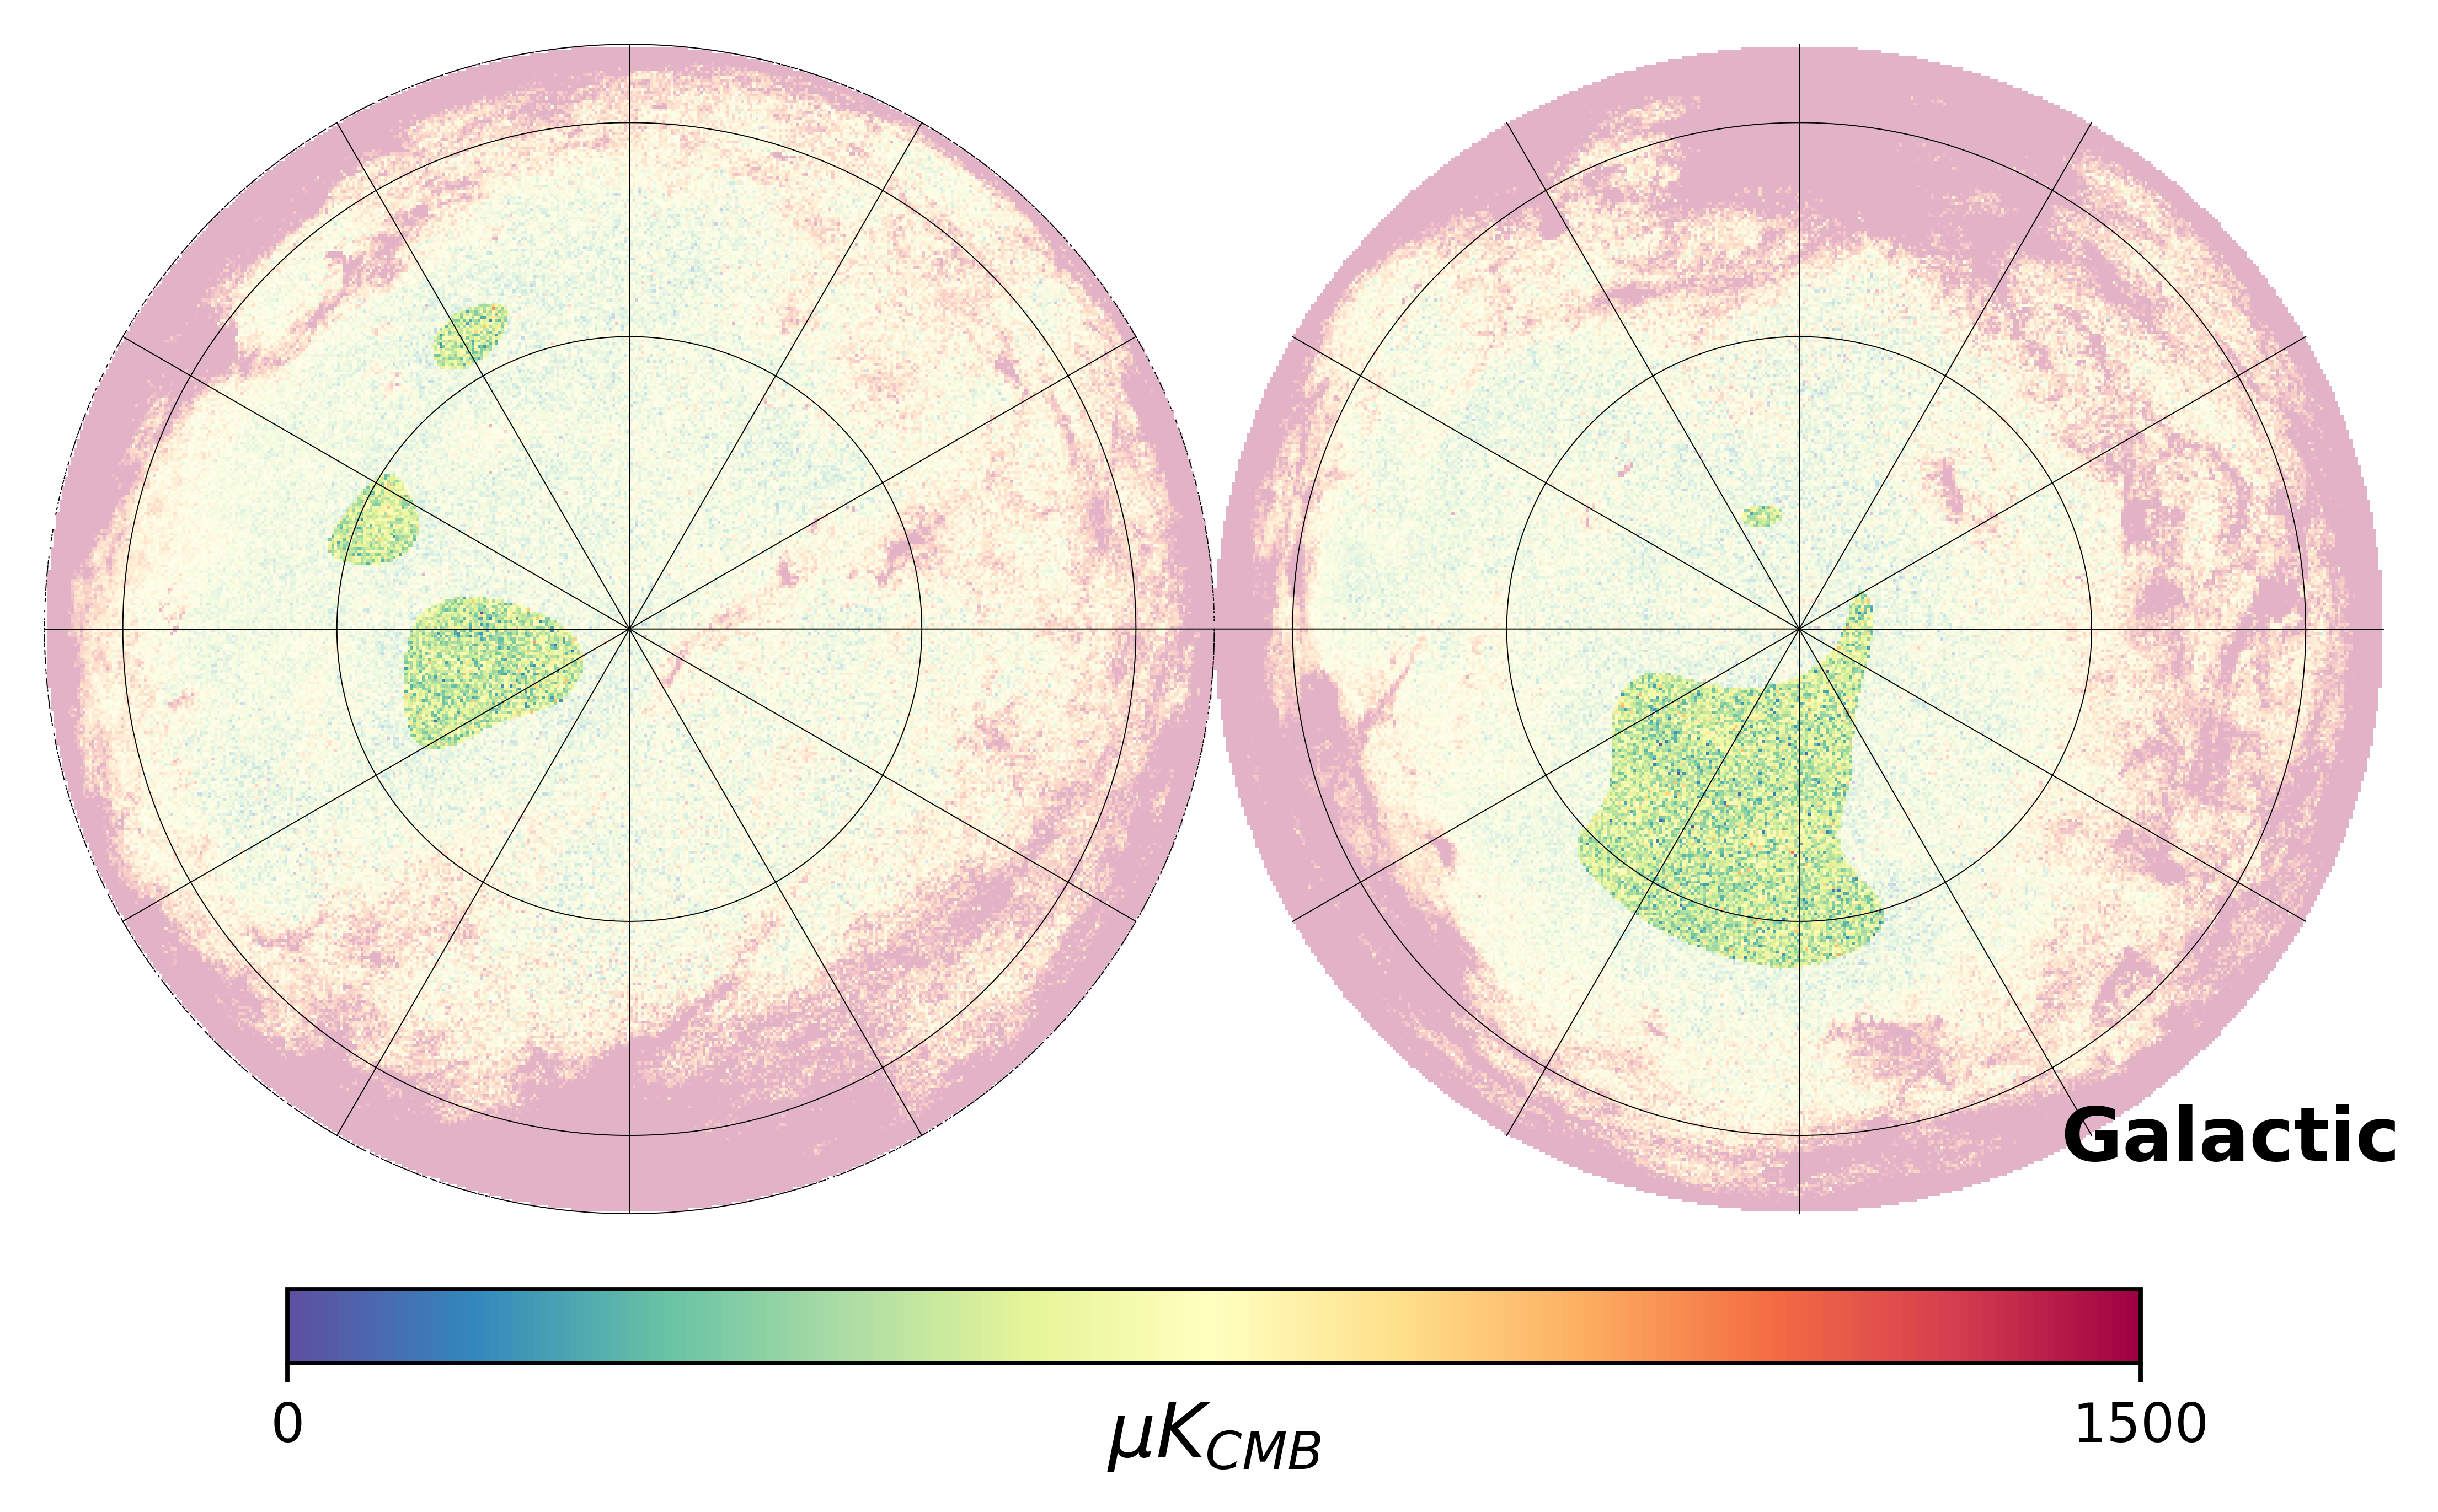
\includegraphics[width=0.44\textwidth]{figures/mask_intxPR3_zero_lvl.png}
    \caption{Mask $\times$ PR3 intensity used to estimate the zero level of PR3 intensity. This mask is obtained by thresholding the intensity of the smoothed PR3 intensity to preserve only the regions where the dust is very low, to estimate the zero-level of the data and models.}
    \label{fig:mask_zero_lvl_int}
\end{figure}

% \begin{figure}
%     \centering
%     \begin{minipage}[c]{0.45\textwidth}
%         \centering
%         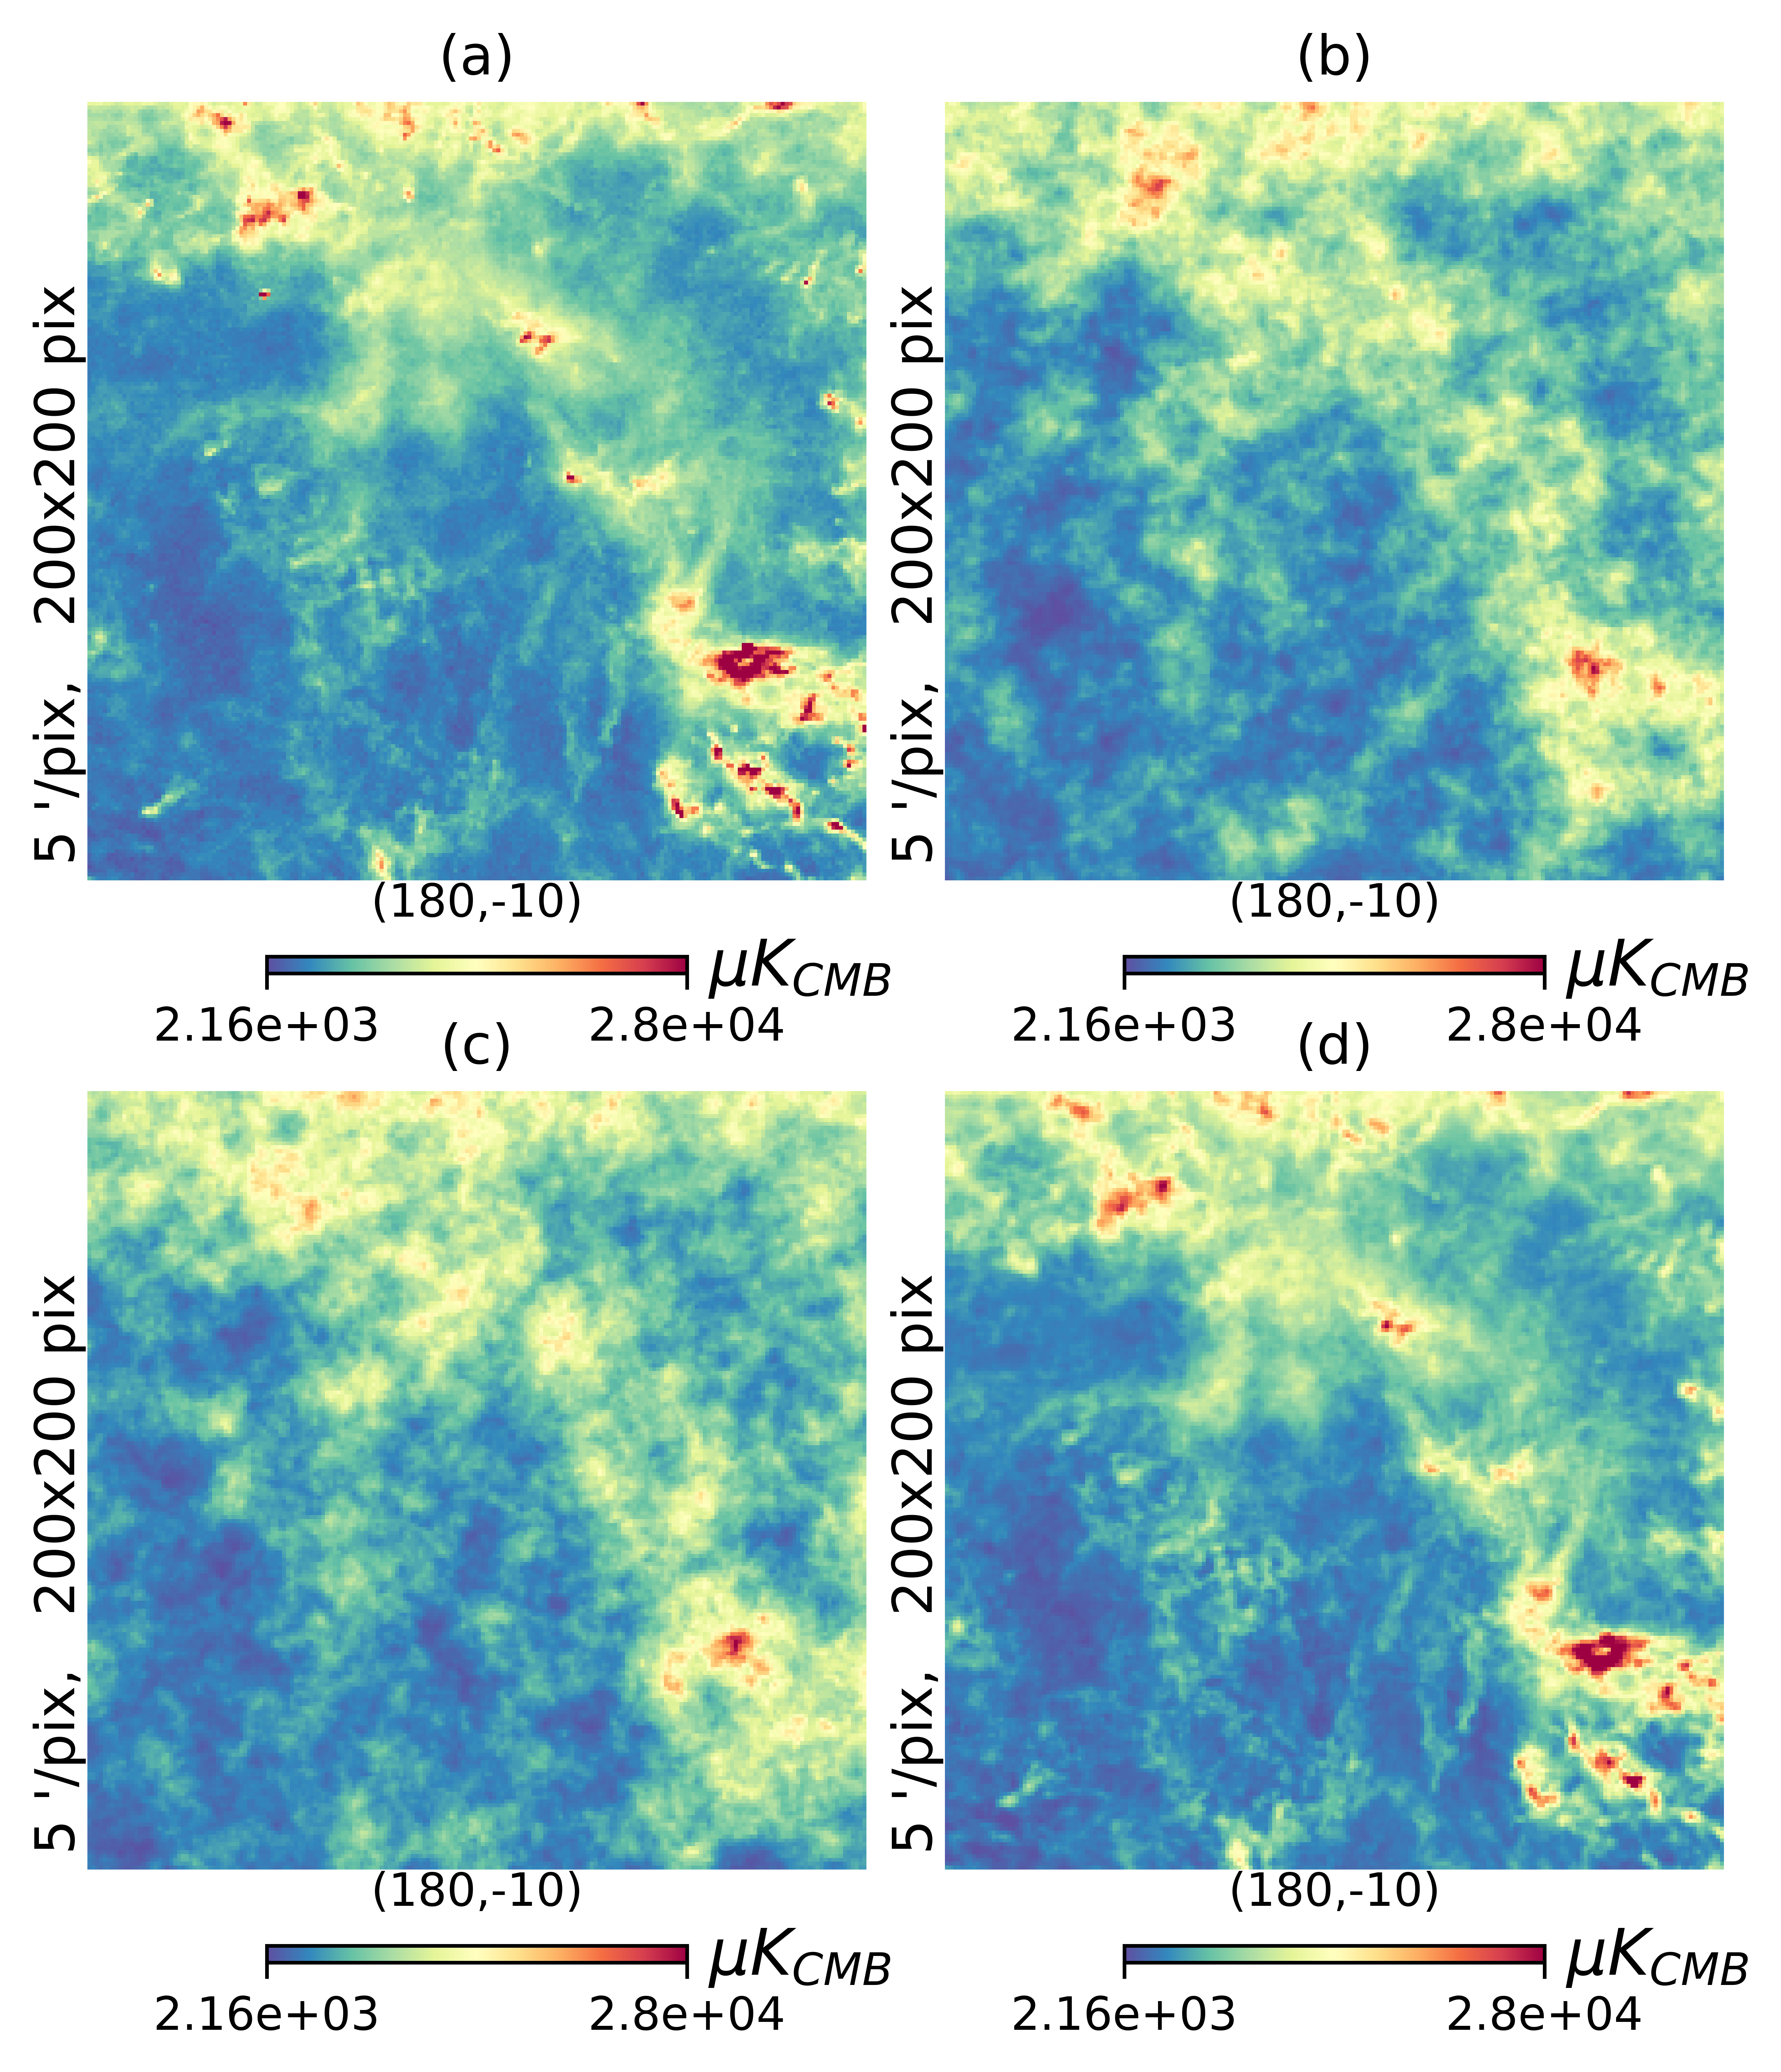
\includegraphics[width=0.45\textwidth]{figures/gal_plane_non_smooth_wo_zero_lvl.png} % first figure itself
%         \caption{Dust intensity at 353GHz at [l = 180, b = -10] with an angular resolution of $4.94\arcmin$: (a) PR3 (b) d1 (c) d9 (d) d12.}
%     \end{minipage}\hfill
%     \begin{minipage}[c]{0.45\textwidth}
%         \centering
%         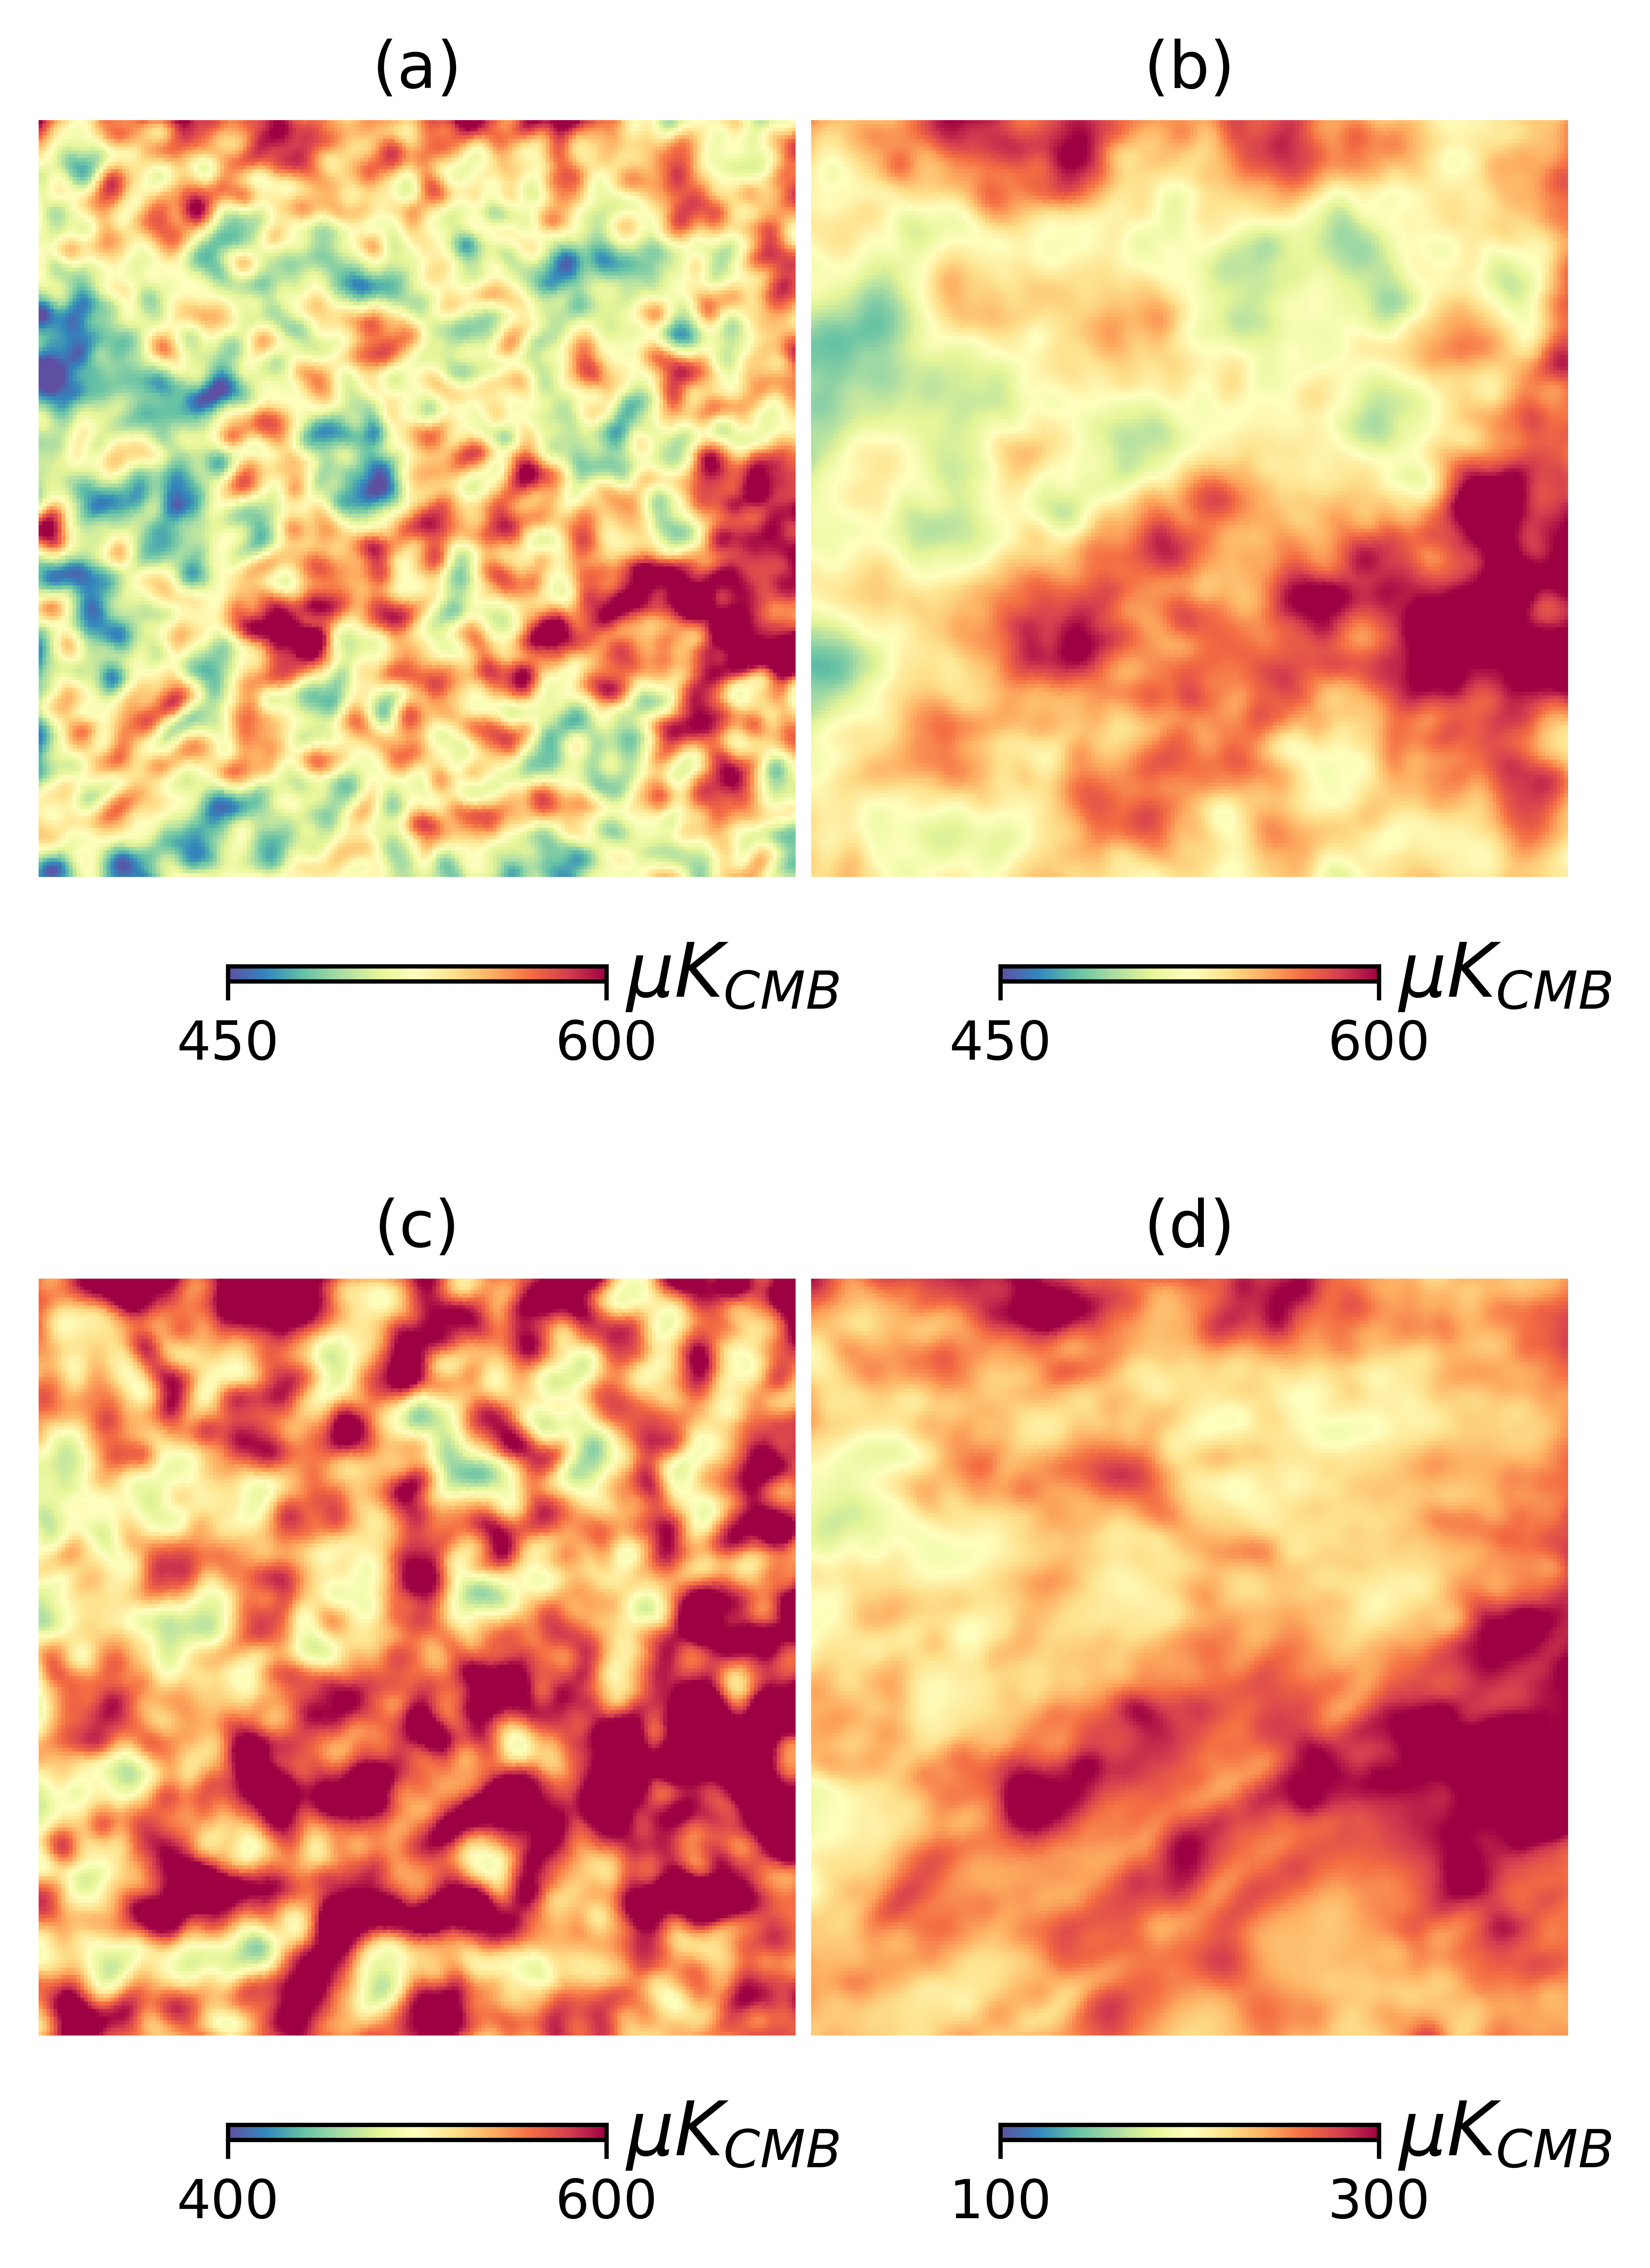
\includegraphics[width=0.45\textwidth]{figures/BK_smooth_30'_wo_zero_lvl.png} % second figure itself
%         \caption{Dust intensity at 353GHz at [l = 318, b = -61] with an angular resolution of $30\arcmin$: (a) PR3 (b) d1 (c) d9 (d) d12. Here, PR3 is contaminated by CIB and extragalactic sources.}
%     \end{minipage}
% \end{figure}

\begin{figure*}[t!]
    \centering
    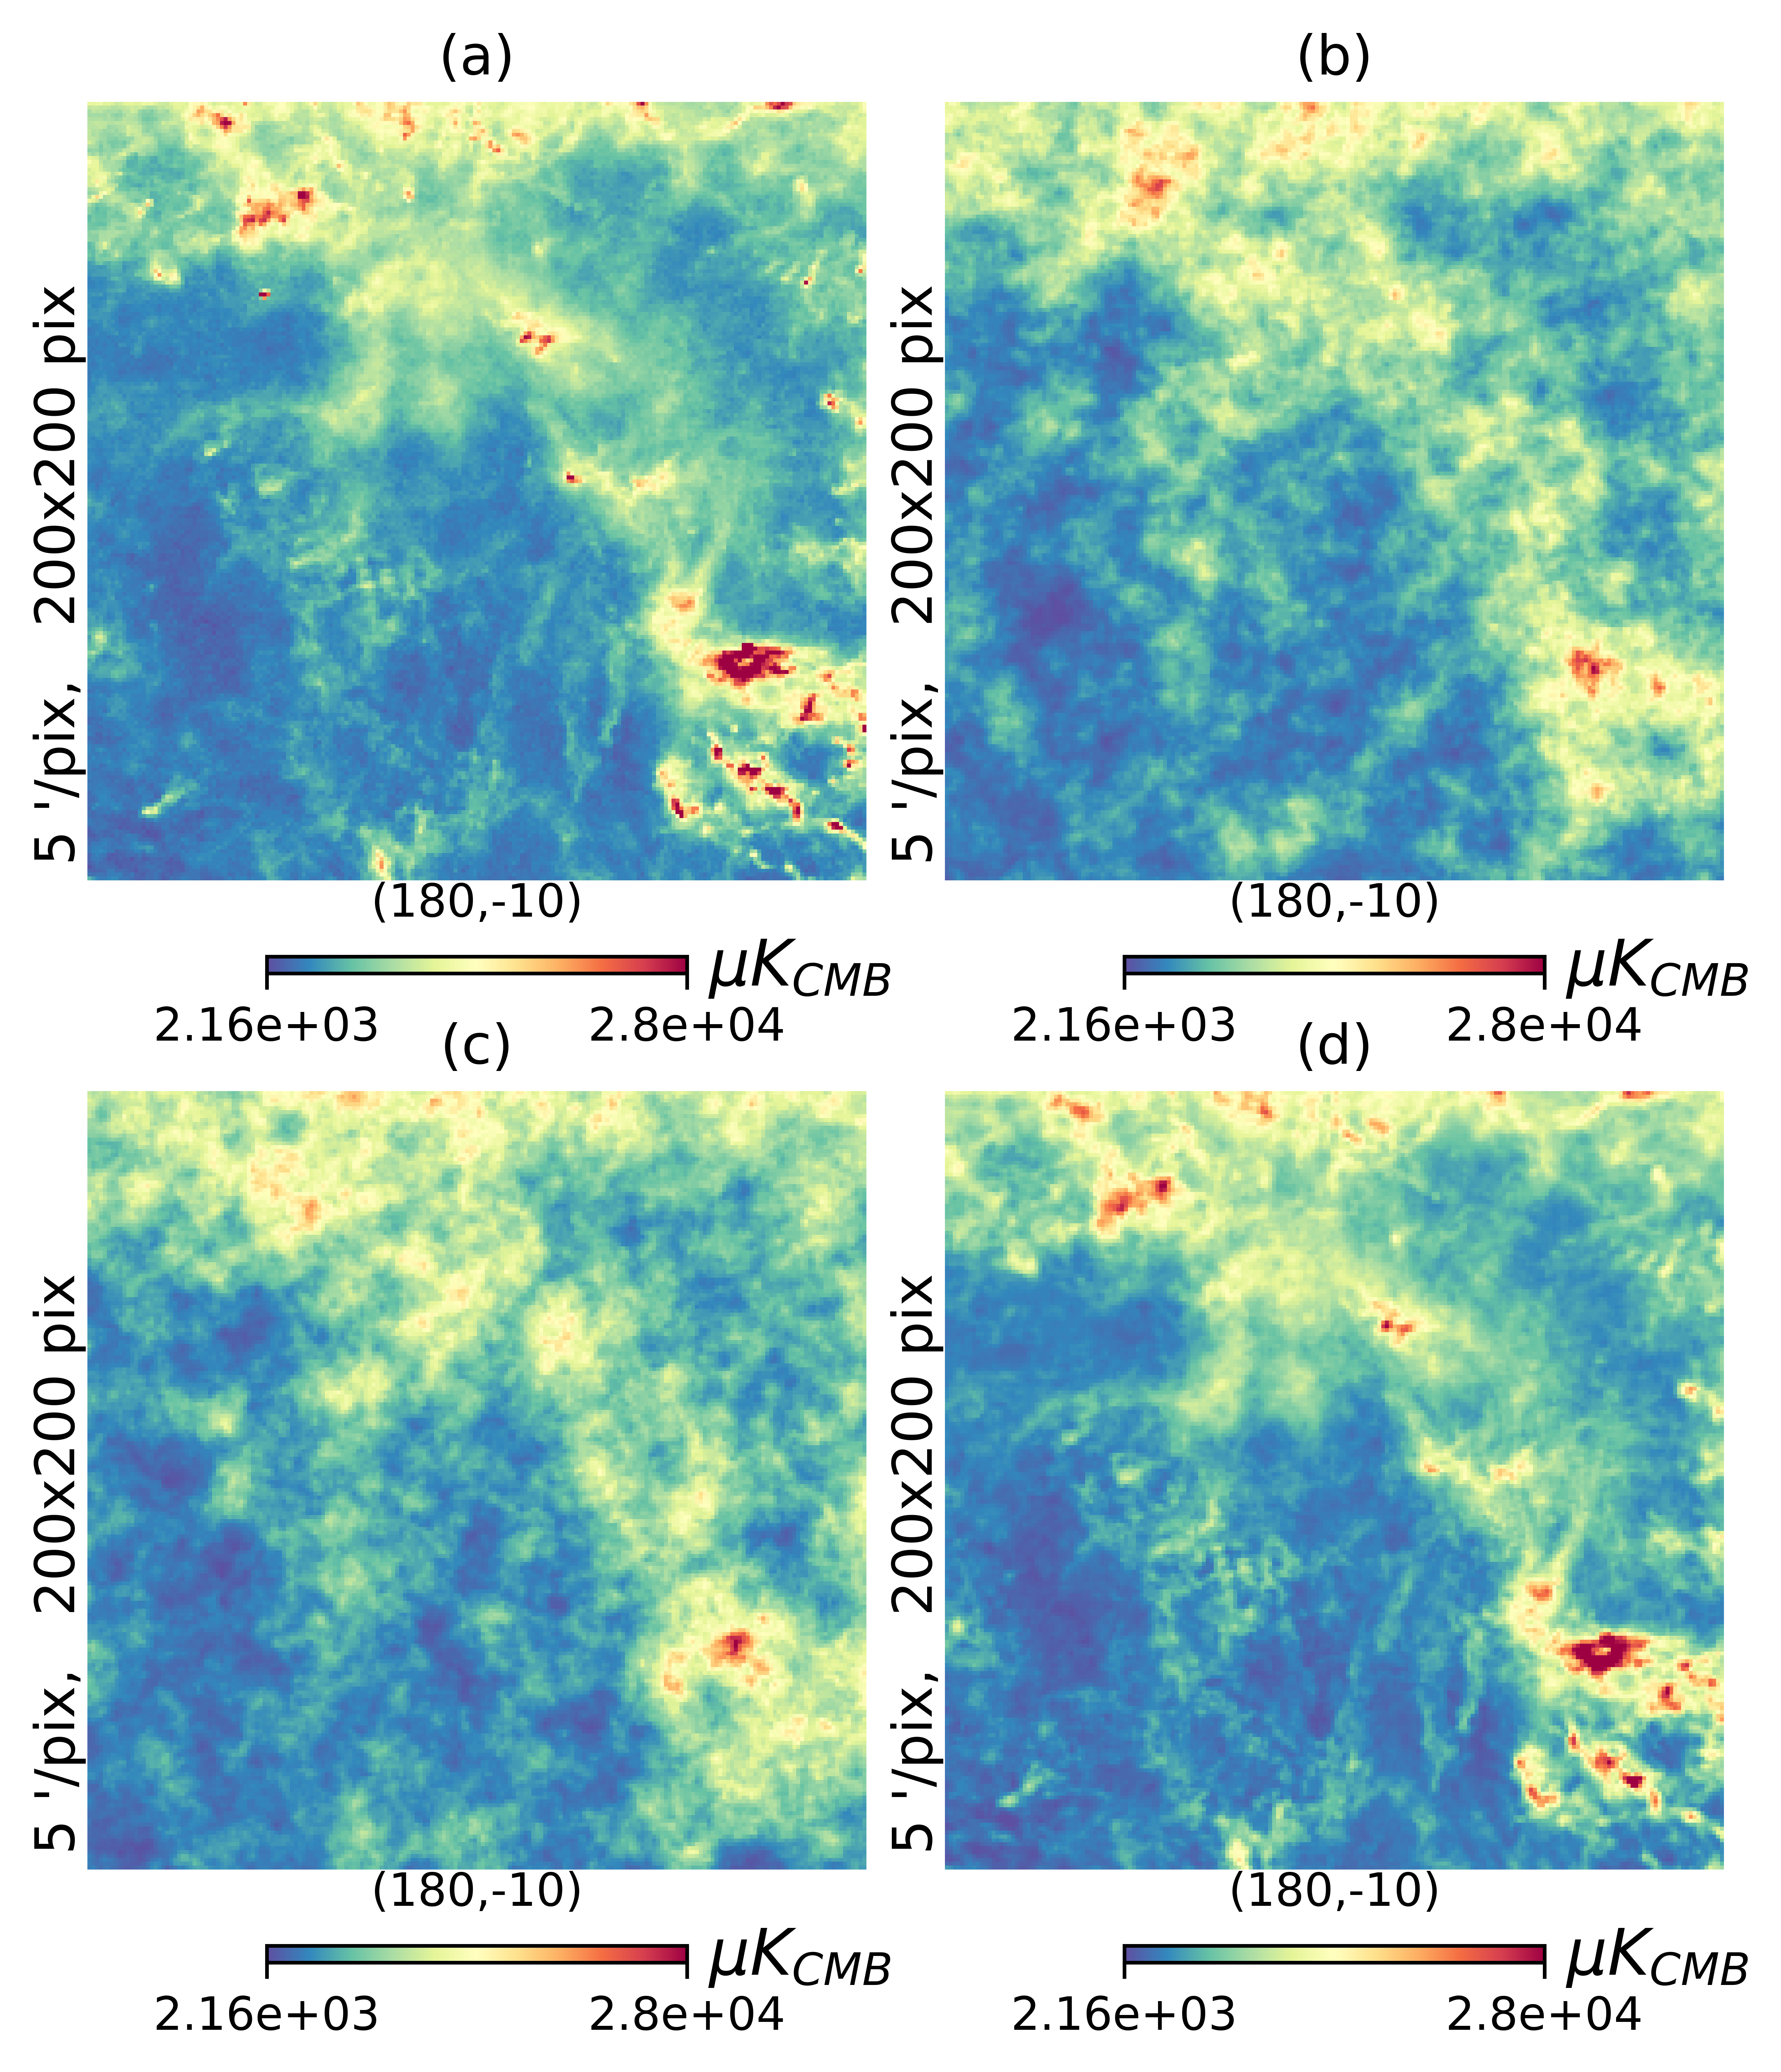
\includegraphics[height=0.4\textwidth]{figures/gal_plane_non_smooth_wo_zero_lvl.png}
    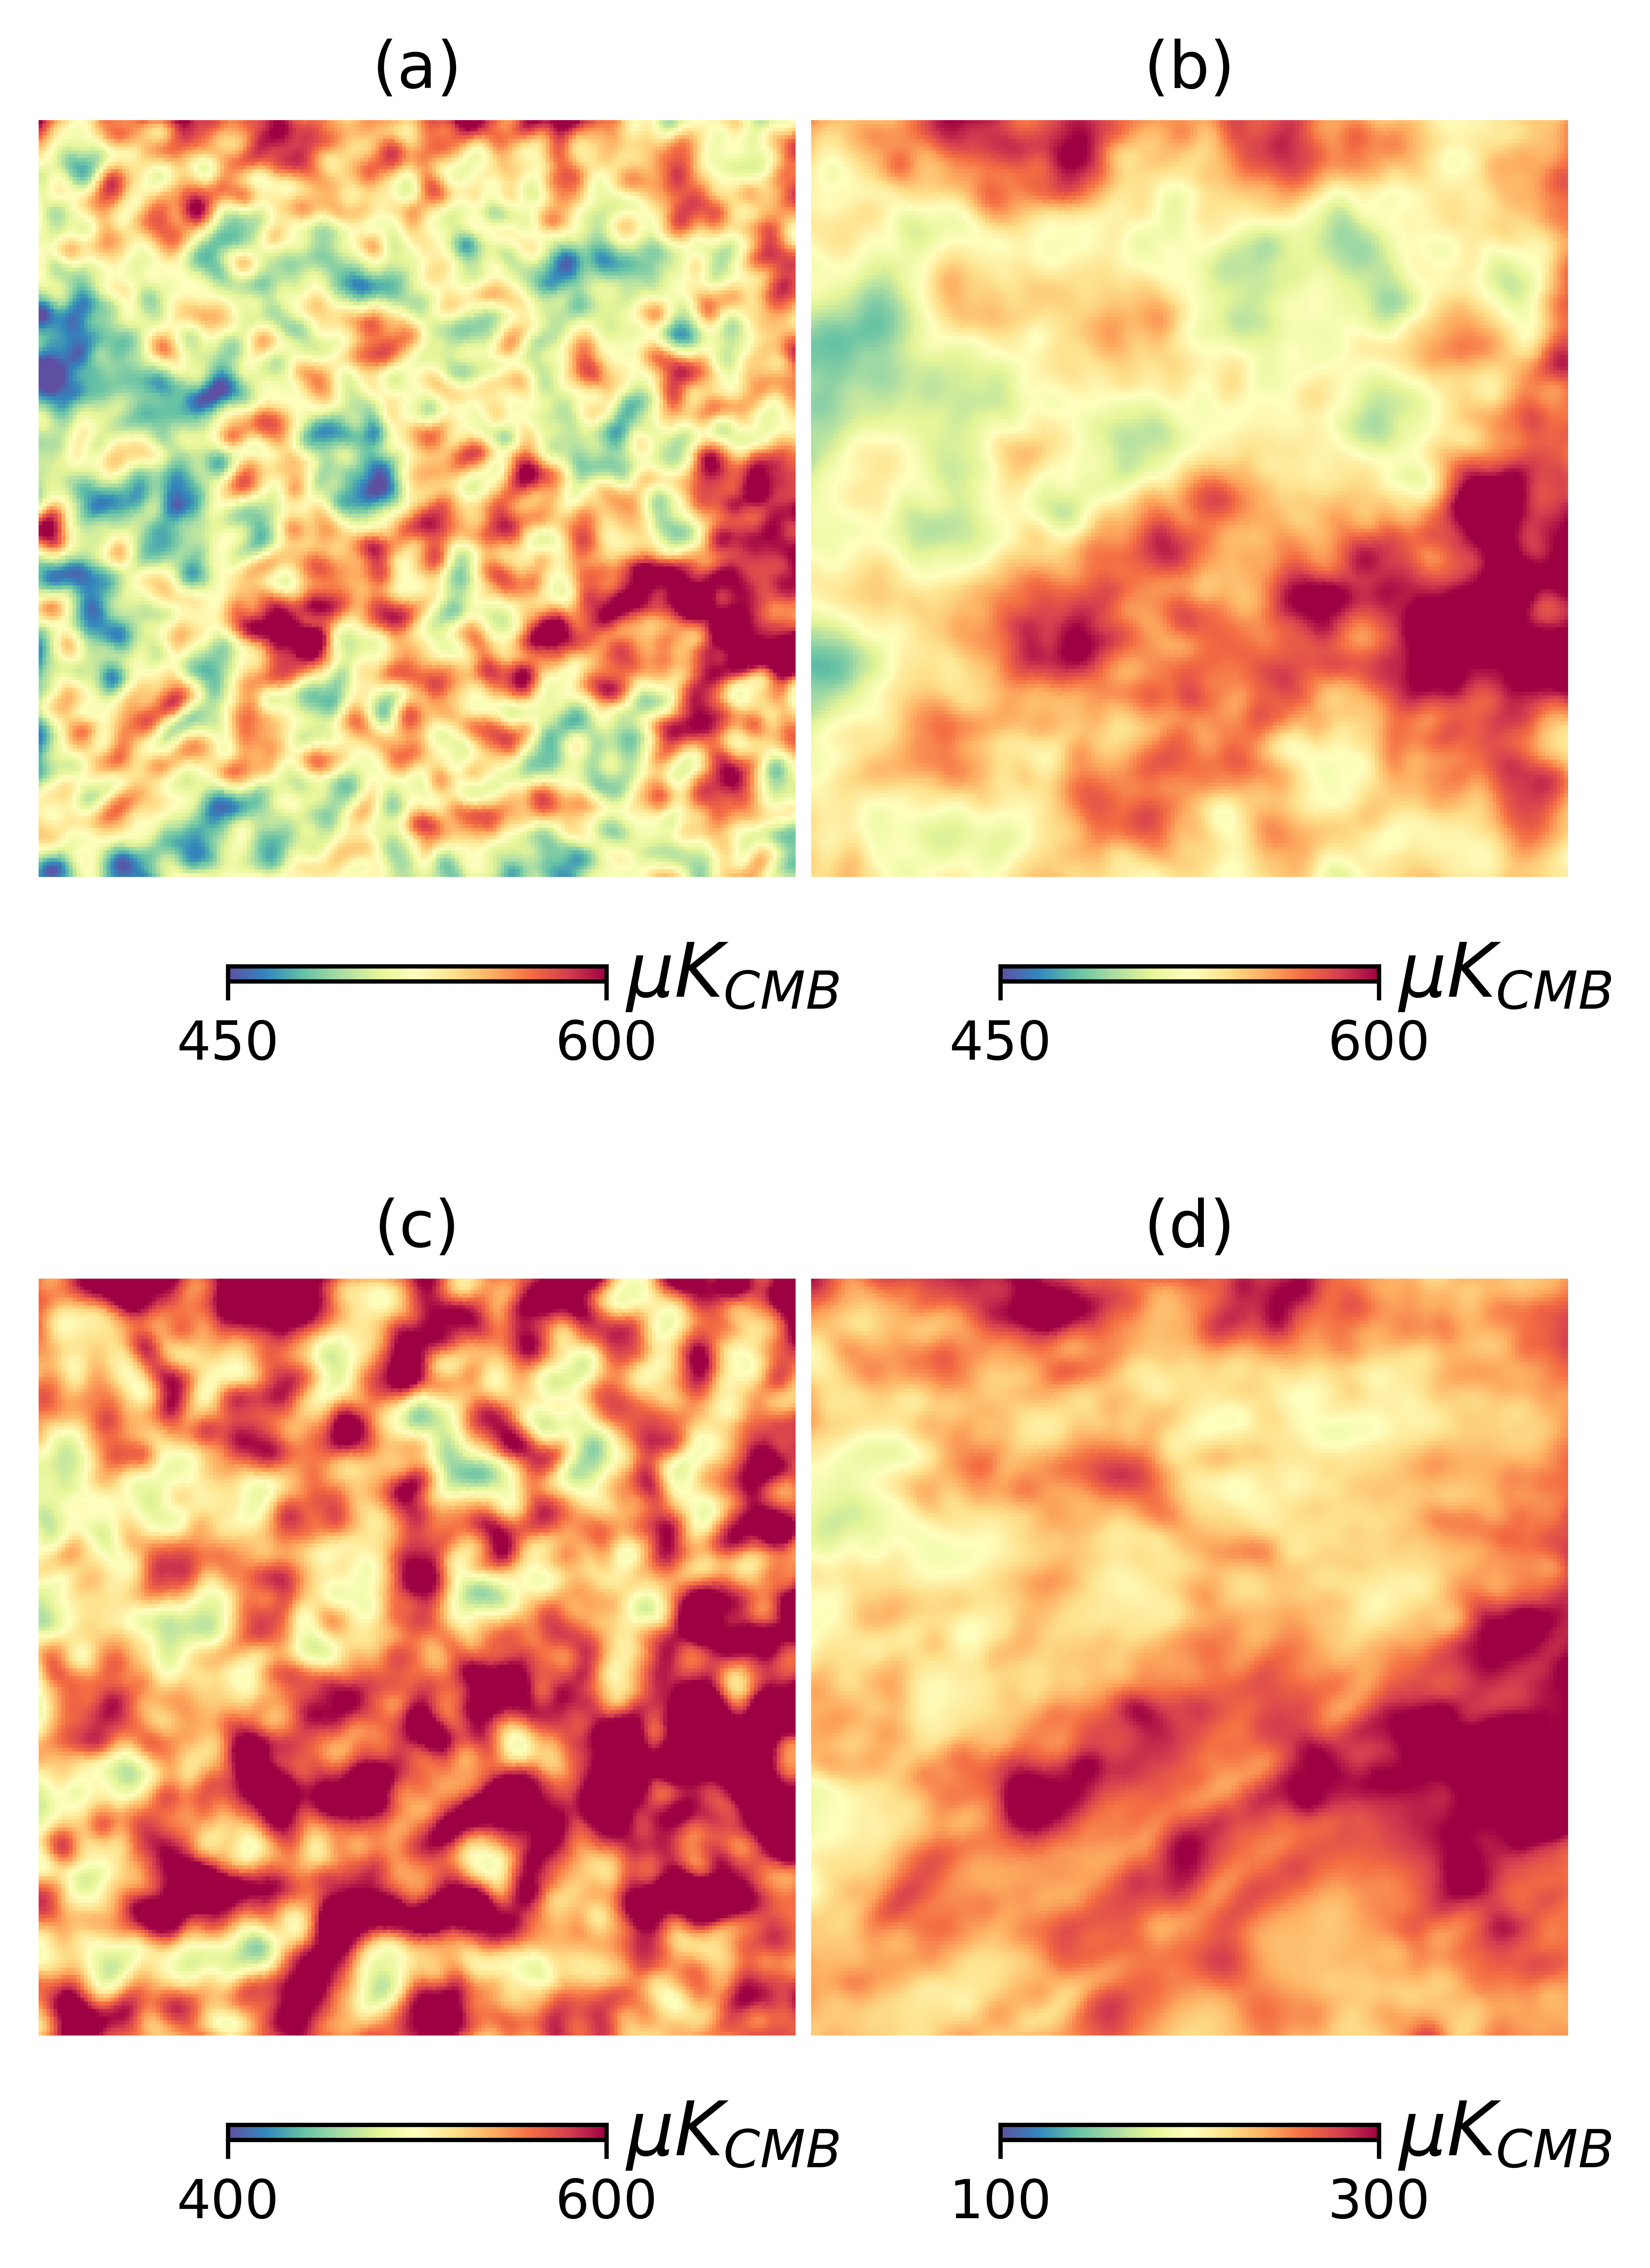
\includegraphics[height=0.4\textwidth]{figures/BK_smooth_30'_wo_zero_lvl.png}
\caption{Dust intensity at 353GHz at [l = 180, b = -10] (left) and [l = 318, b = -61] (right) with an angular resolution of $4.94\arcmin$: (a) PR3 (b) d1 (c) d9 (d) d12.}    
\label{fig:353_int}
\end{figure*}
% \begin{figure}
%     \centering
%     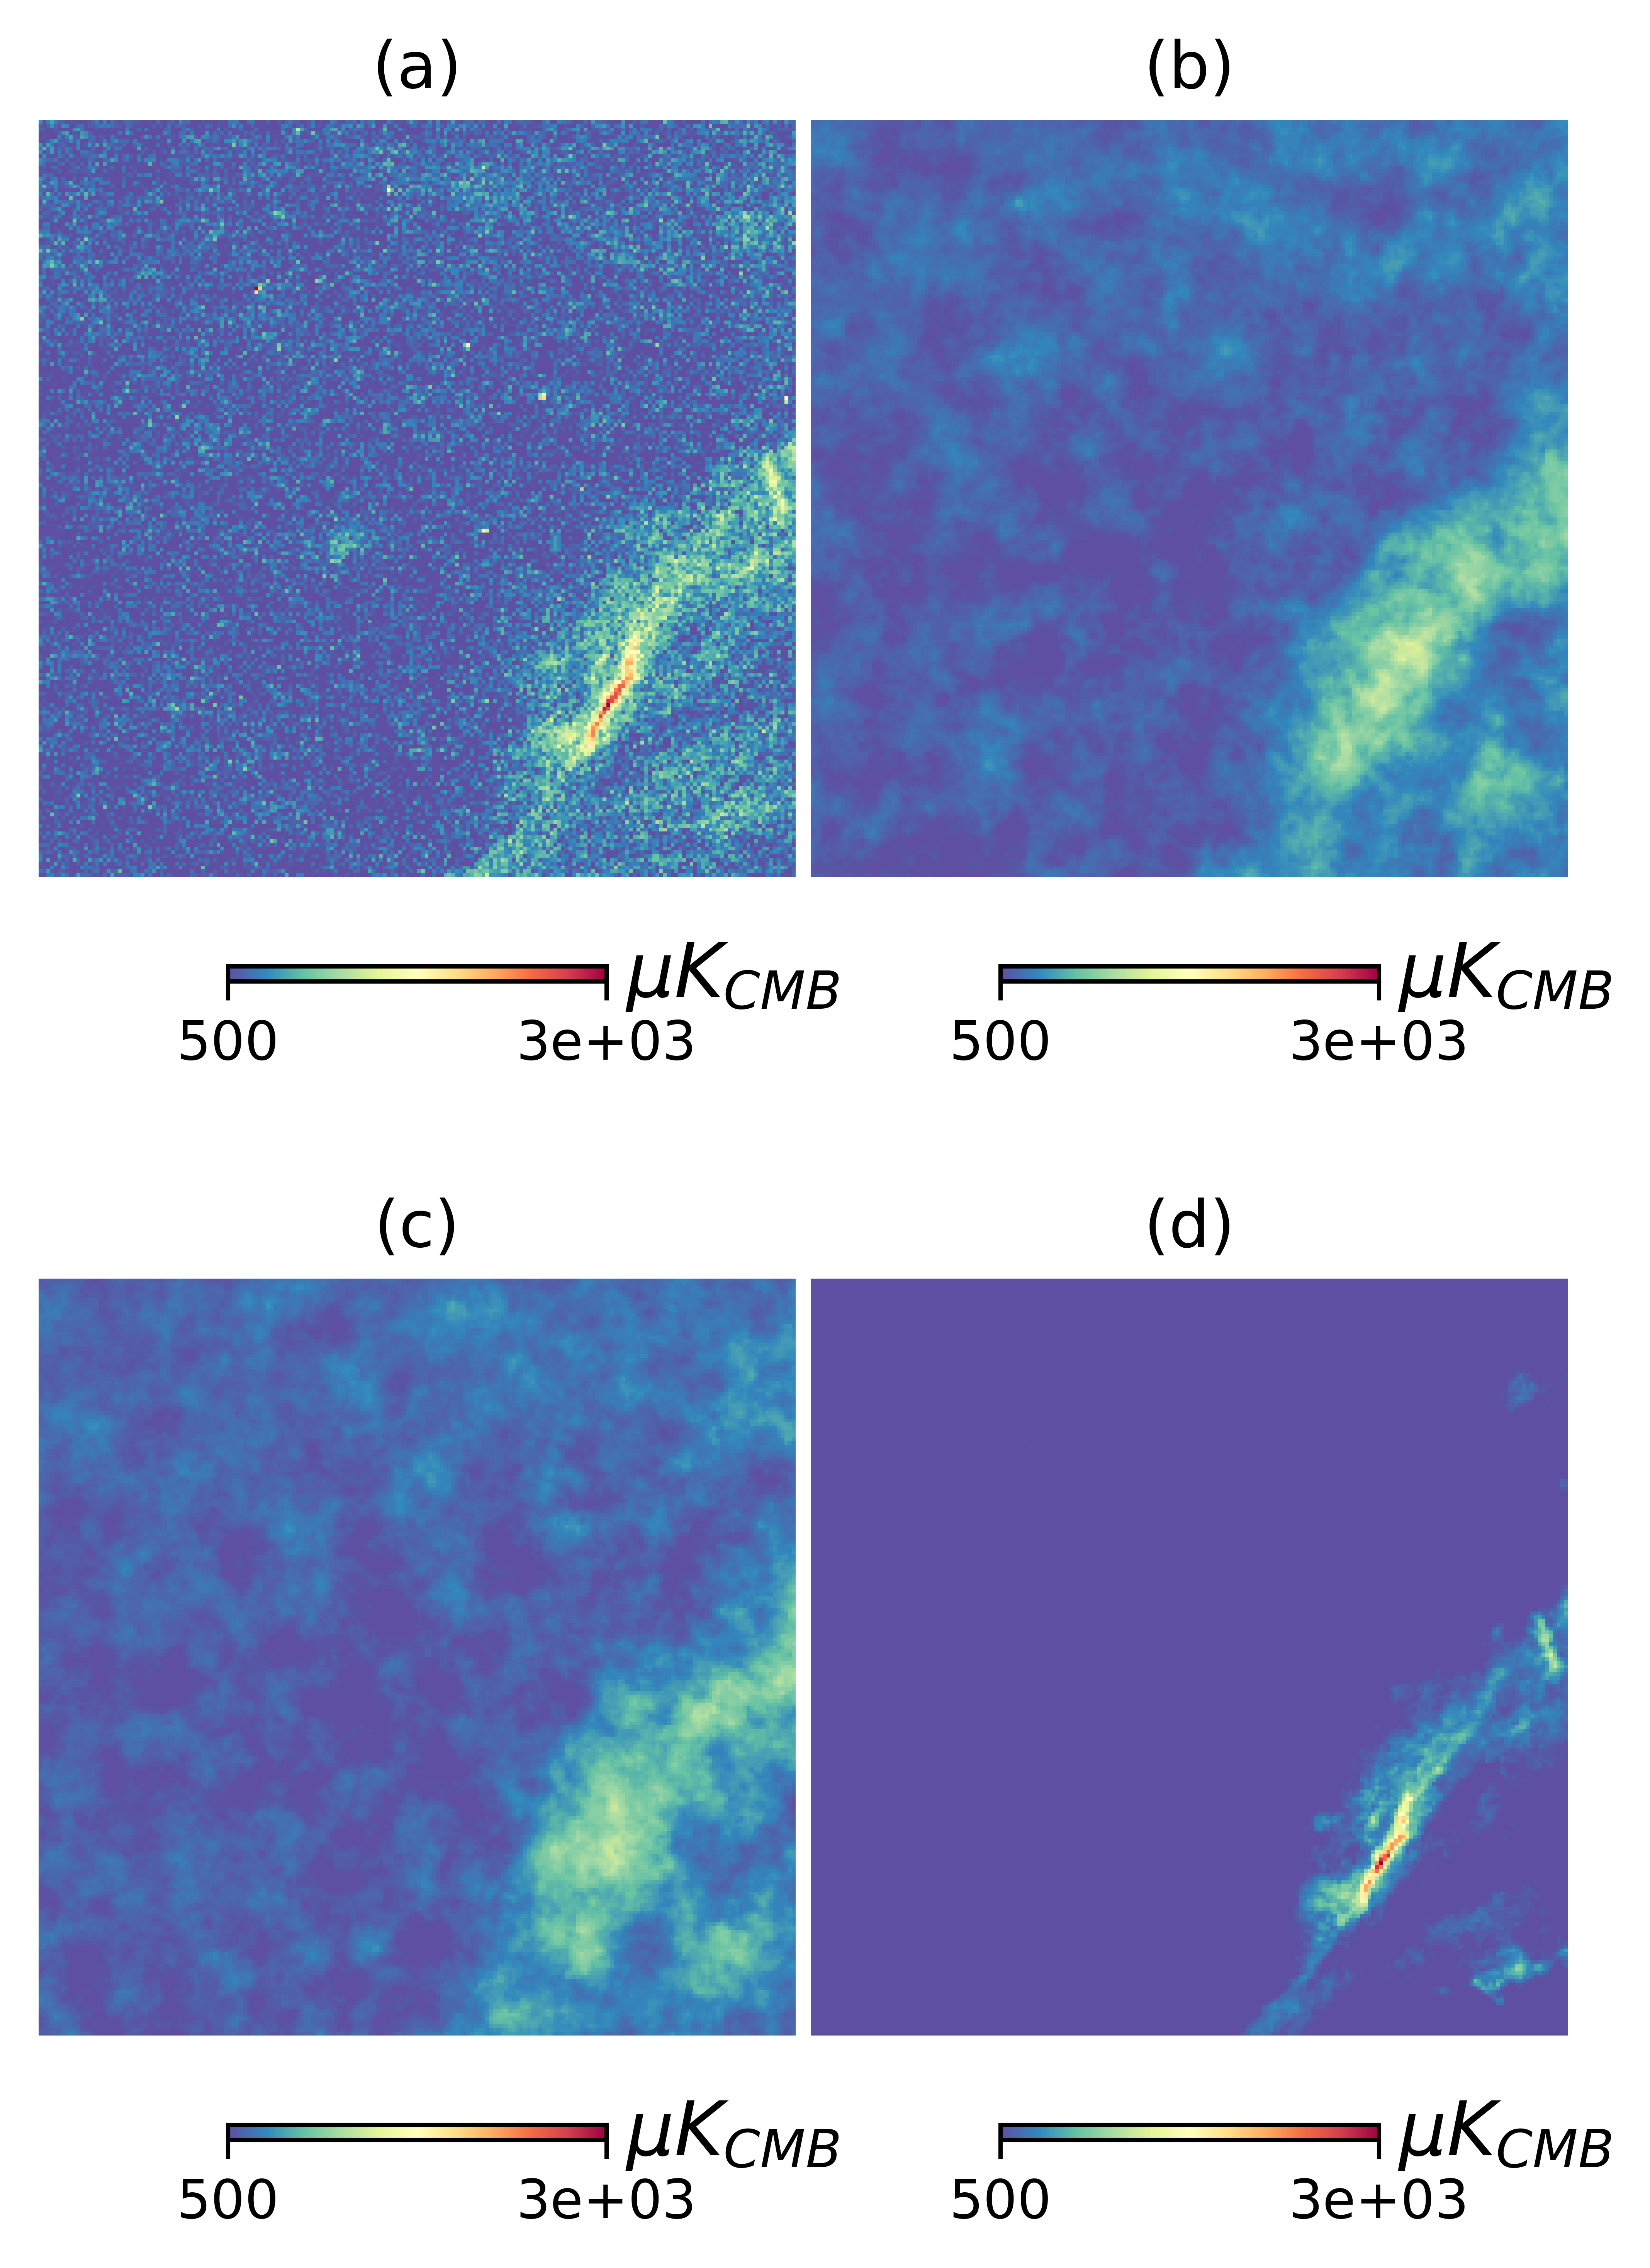
\includegraphics[scale = 0.6]{figures/NGP_non_smooth_wo_zero_lvl.png}
%     \caption{Dust intensity at 353GHz centered at [l = 0, b = 90]: (a) PR3 (b) d9 (c) d11 (d) d12}
%     \label{fig:353_int_NP}
% \end{figure}
% \begin{figure}[ht!]
%     \centering
%     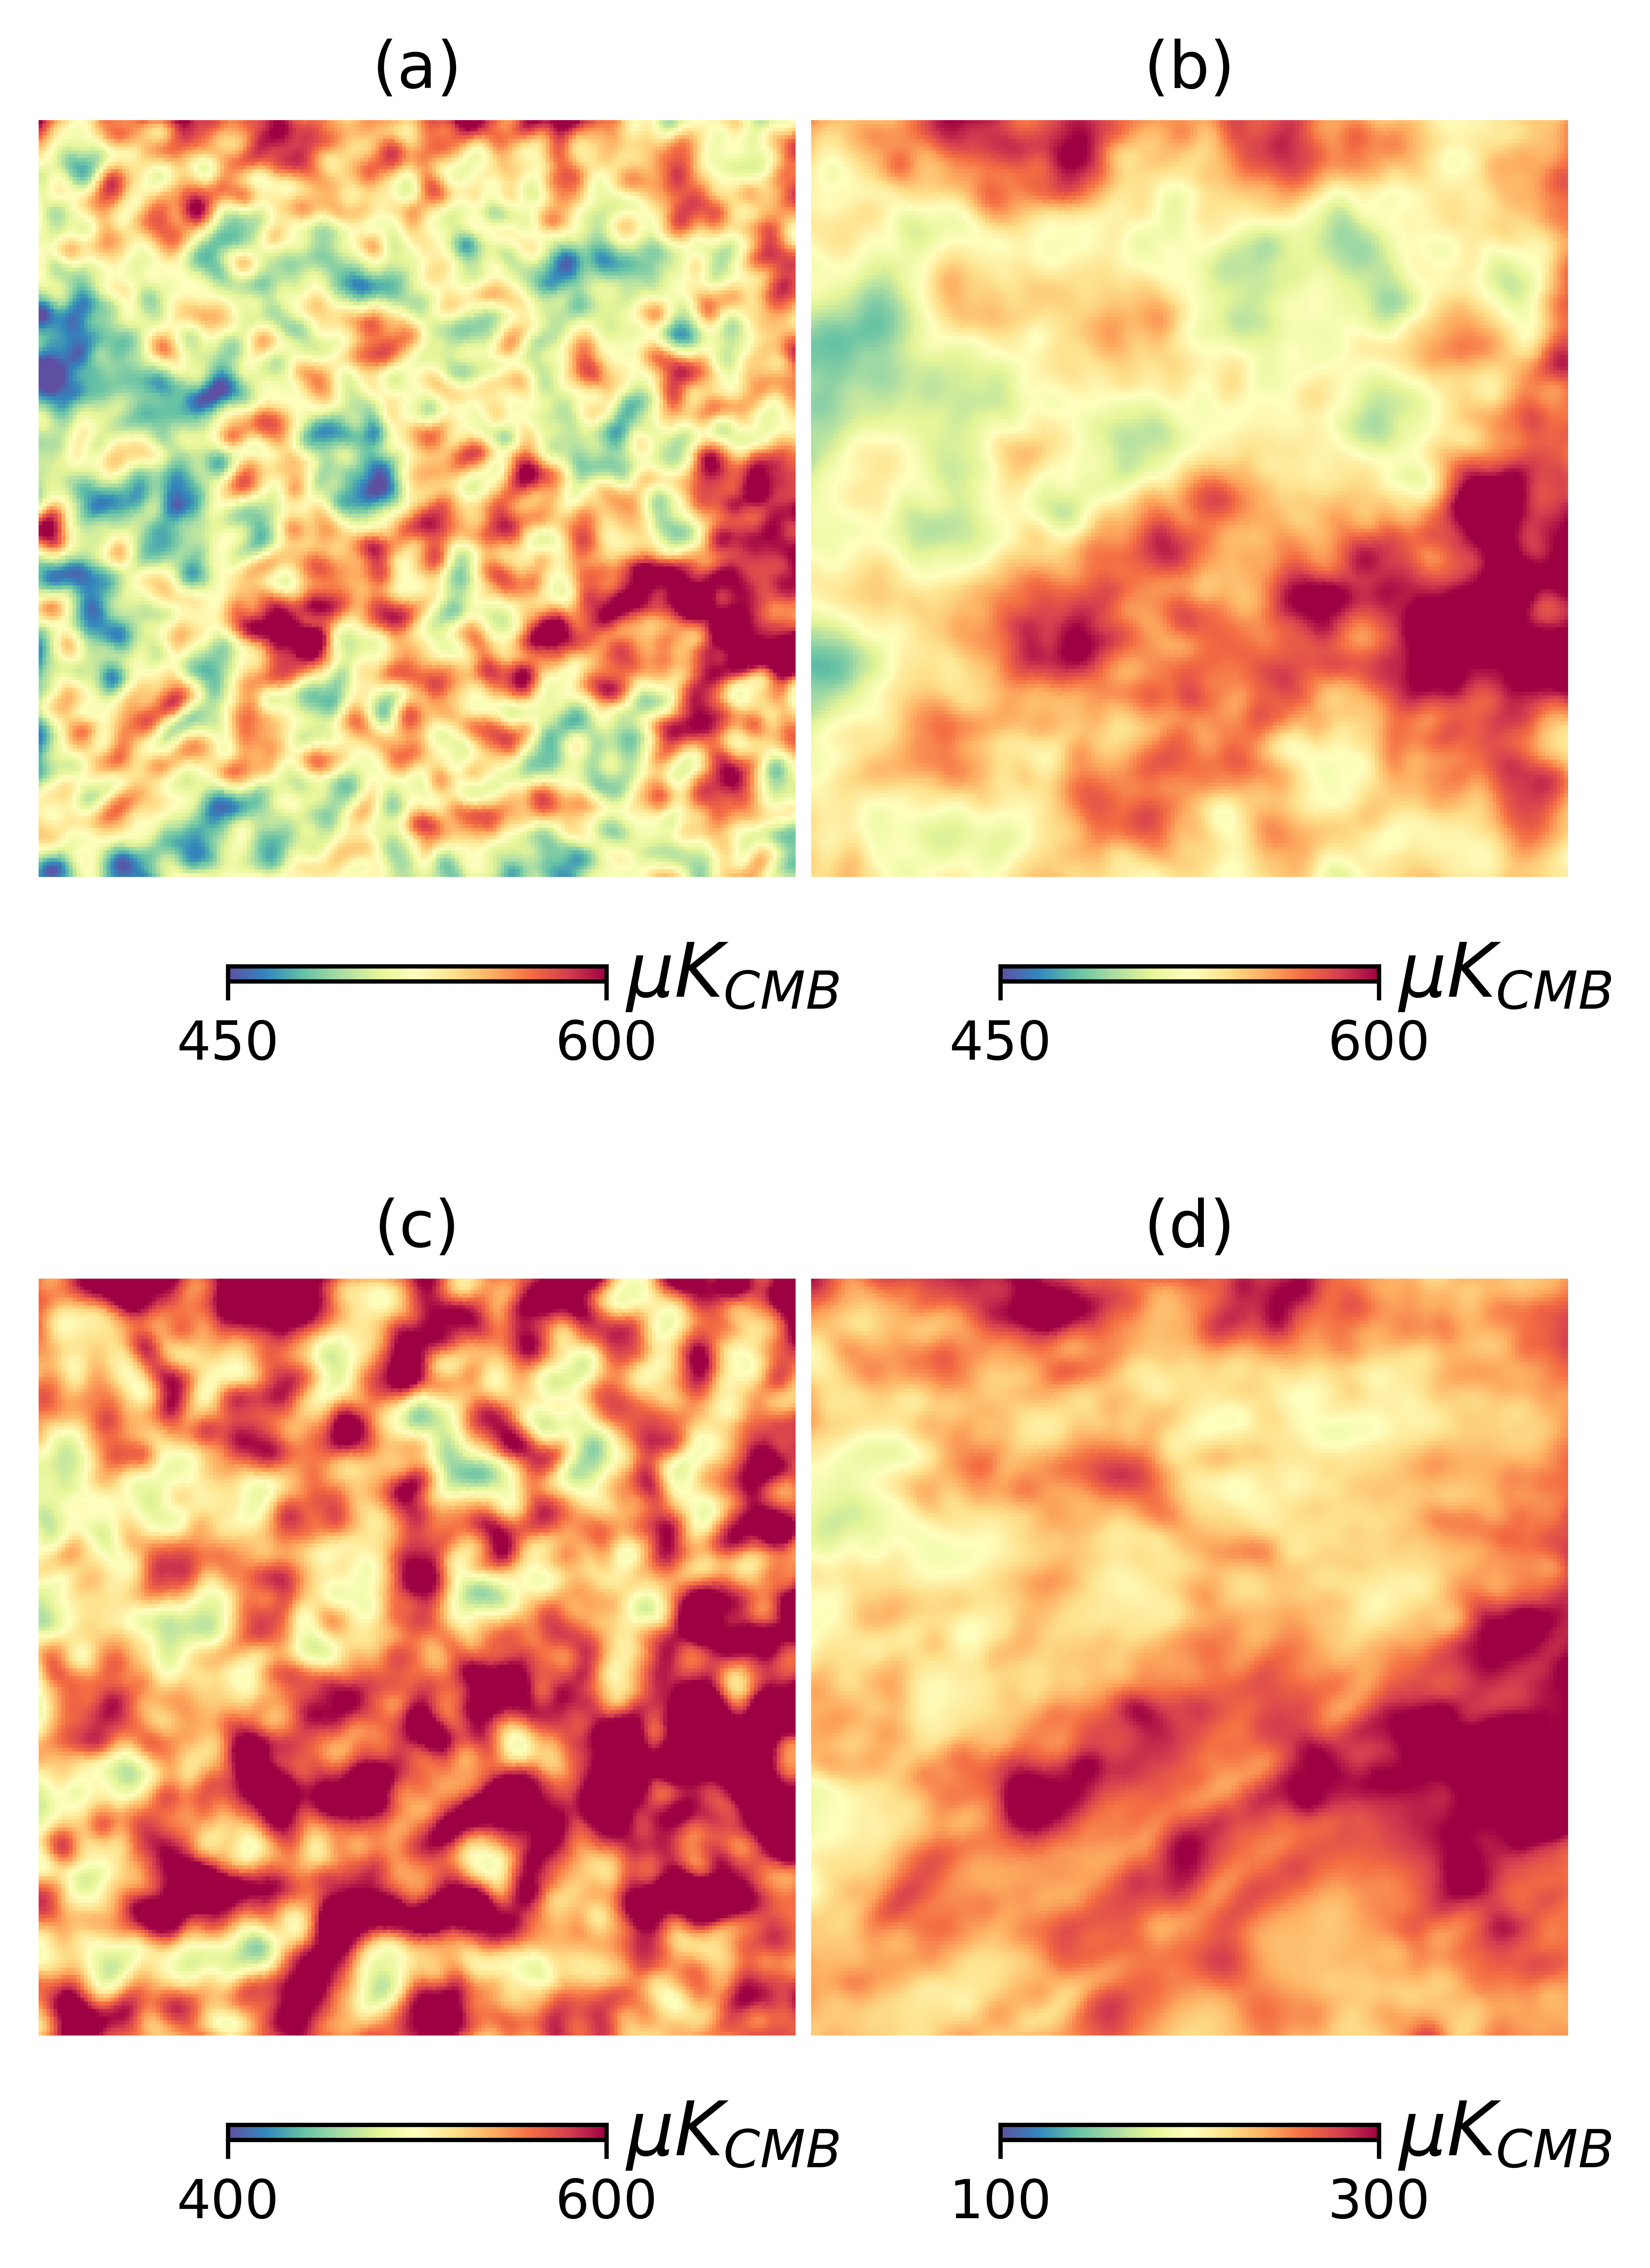
\includegraphics[width=0.5\textwidth]{figures/BK_smooth_30'_wo_zero_lvl.png}
%     \caption{Dust intensity at 353GHz at [l = 318, b = -61] with an angular resolution of $30\arcmin$: (a) PR3 (b) d1 (c) d9 (d) d12. Here, PR3 is contaminated by CIB and extragalactic sources.}
%     \label{fig:353_int_BK}
% \end{figure}

\begin{figure*}[t!]
    \centering
    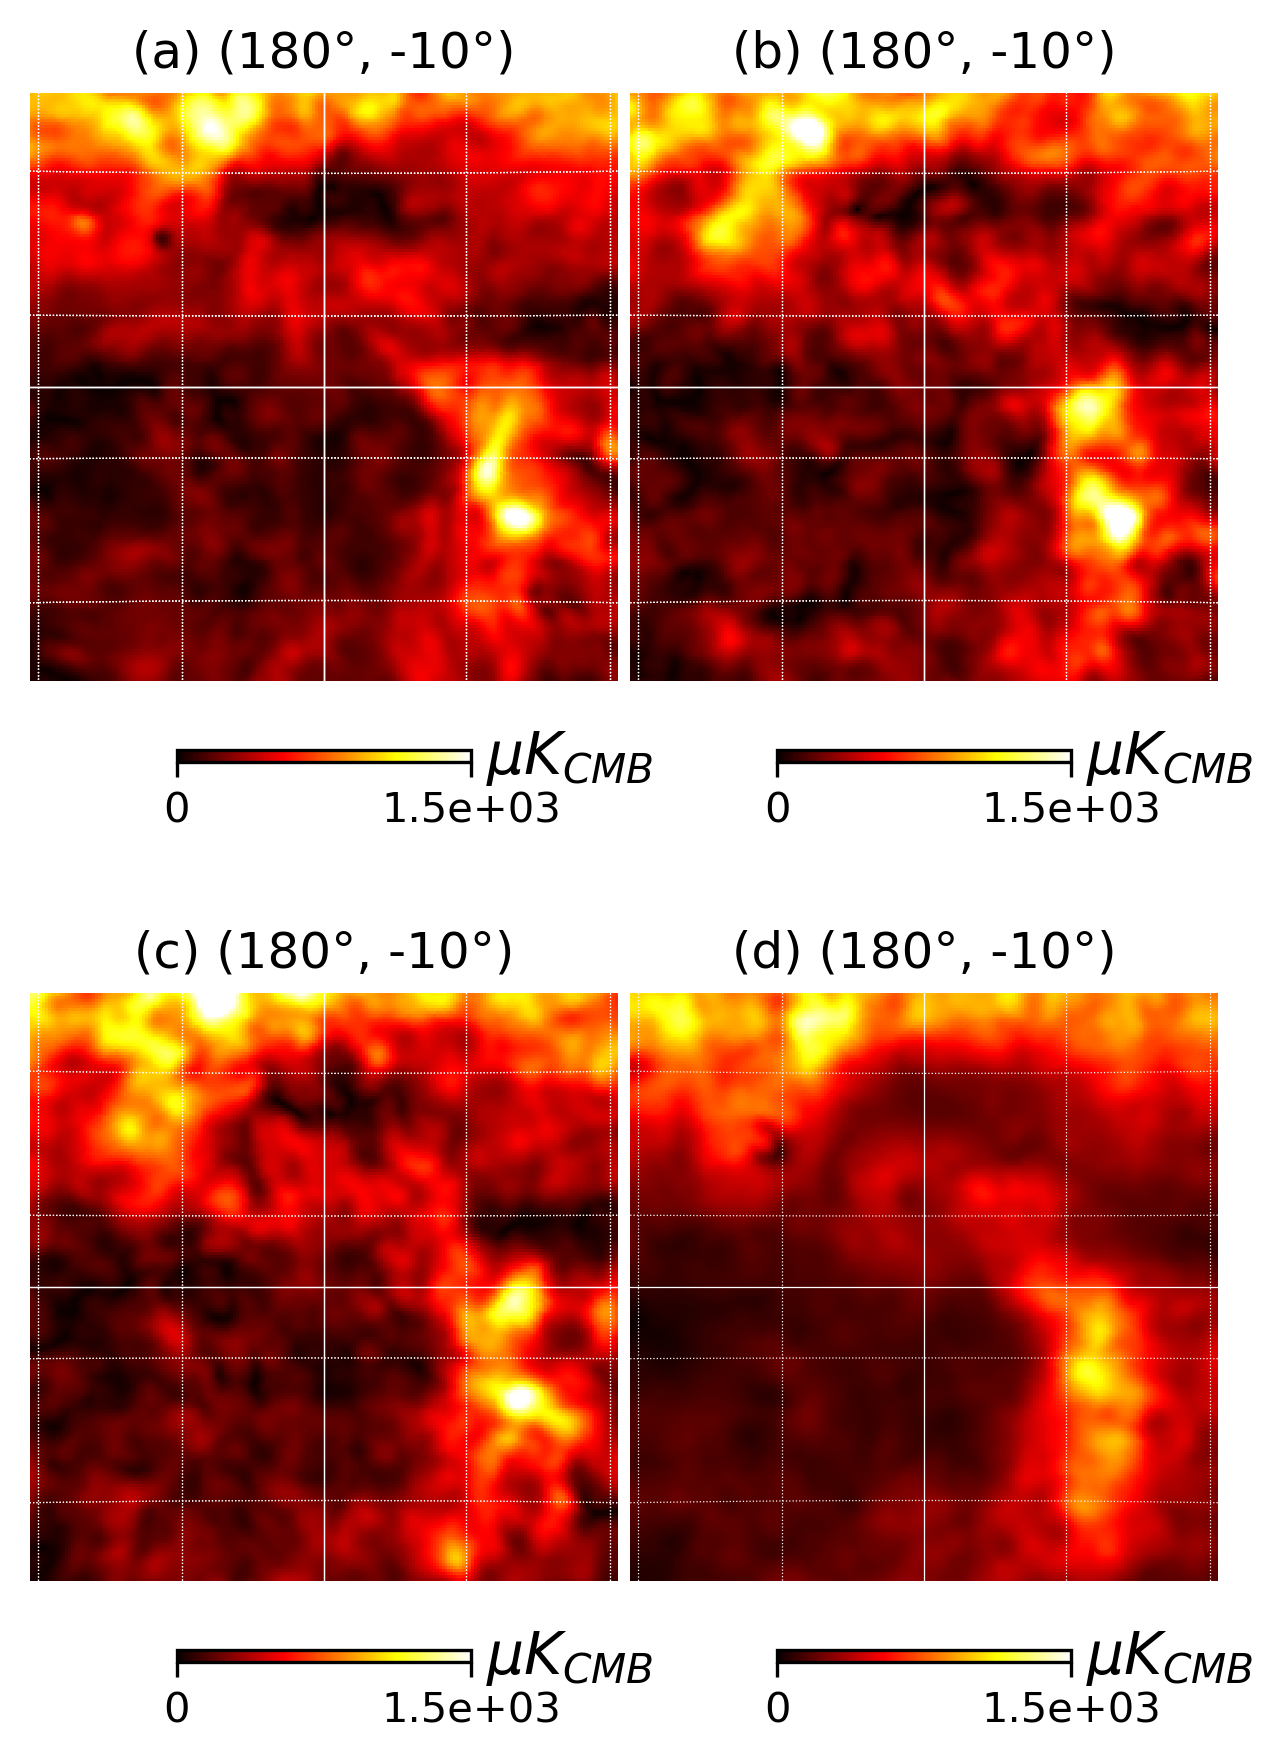
\includegraphics[height=0.41\textwidth]{figures/pol_gal_plane_smooth_30'.png}
    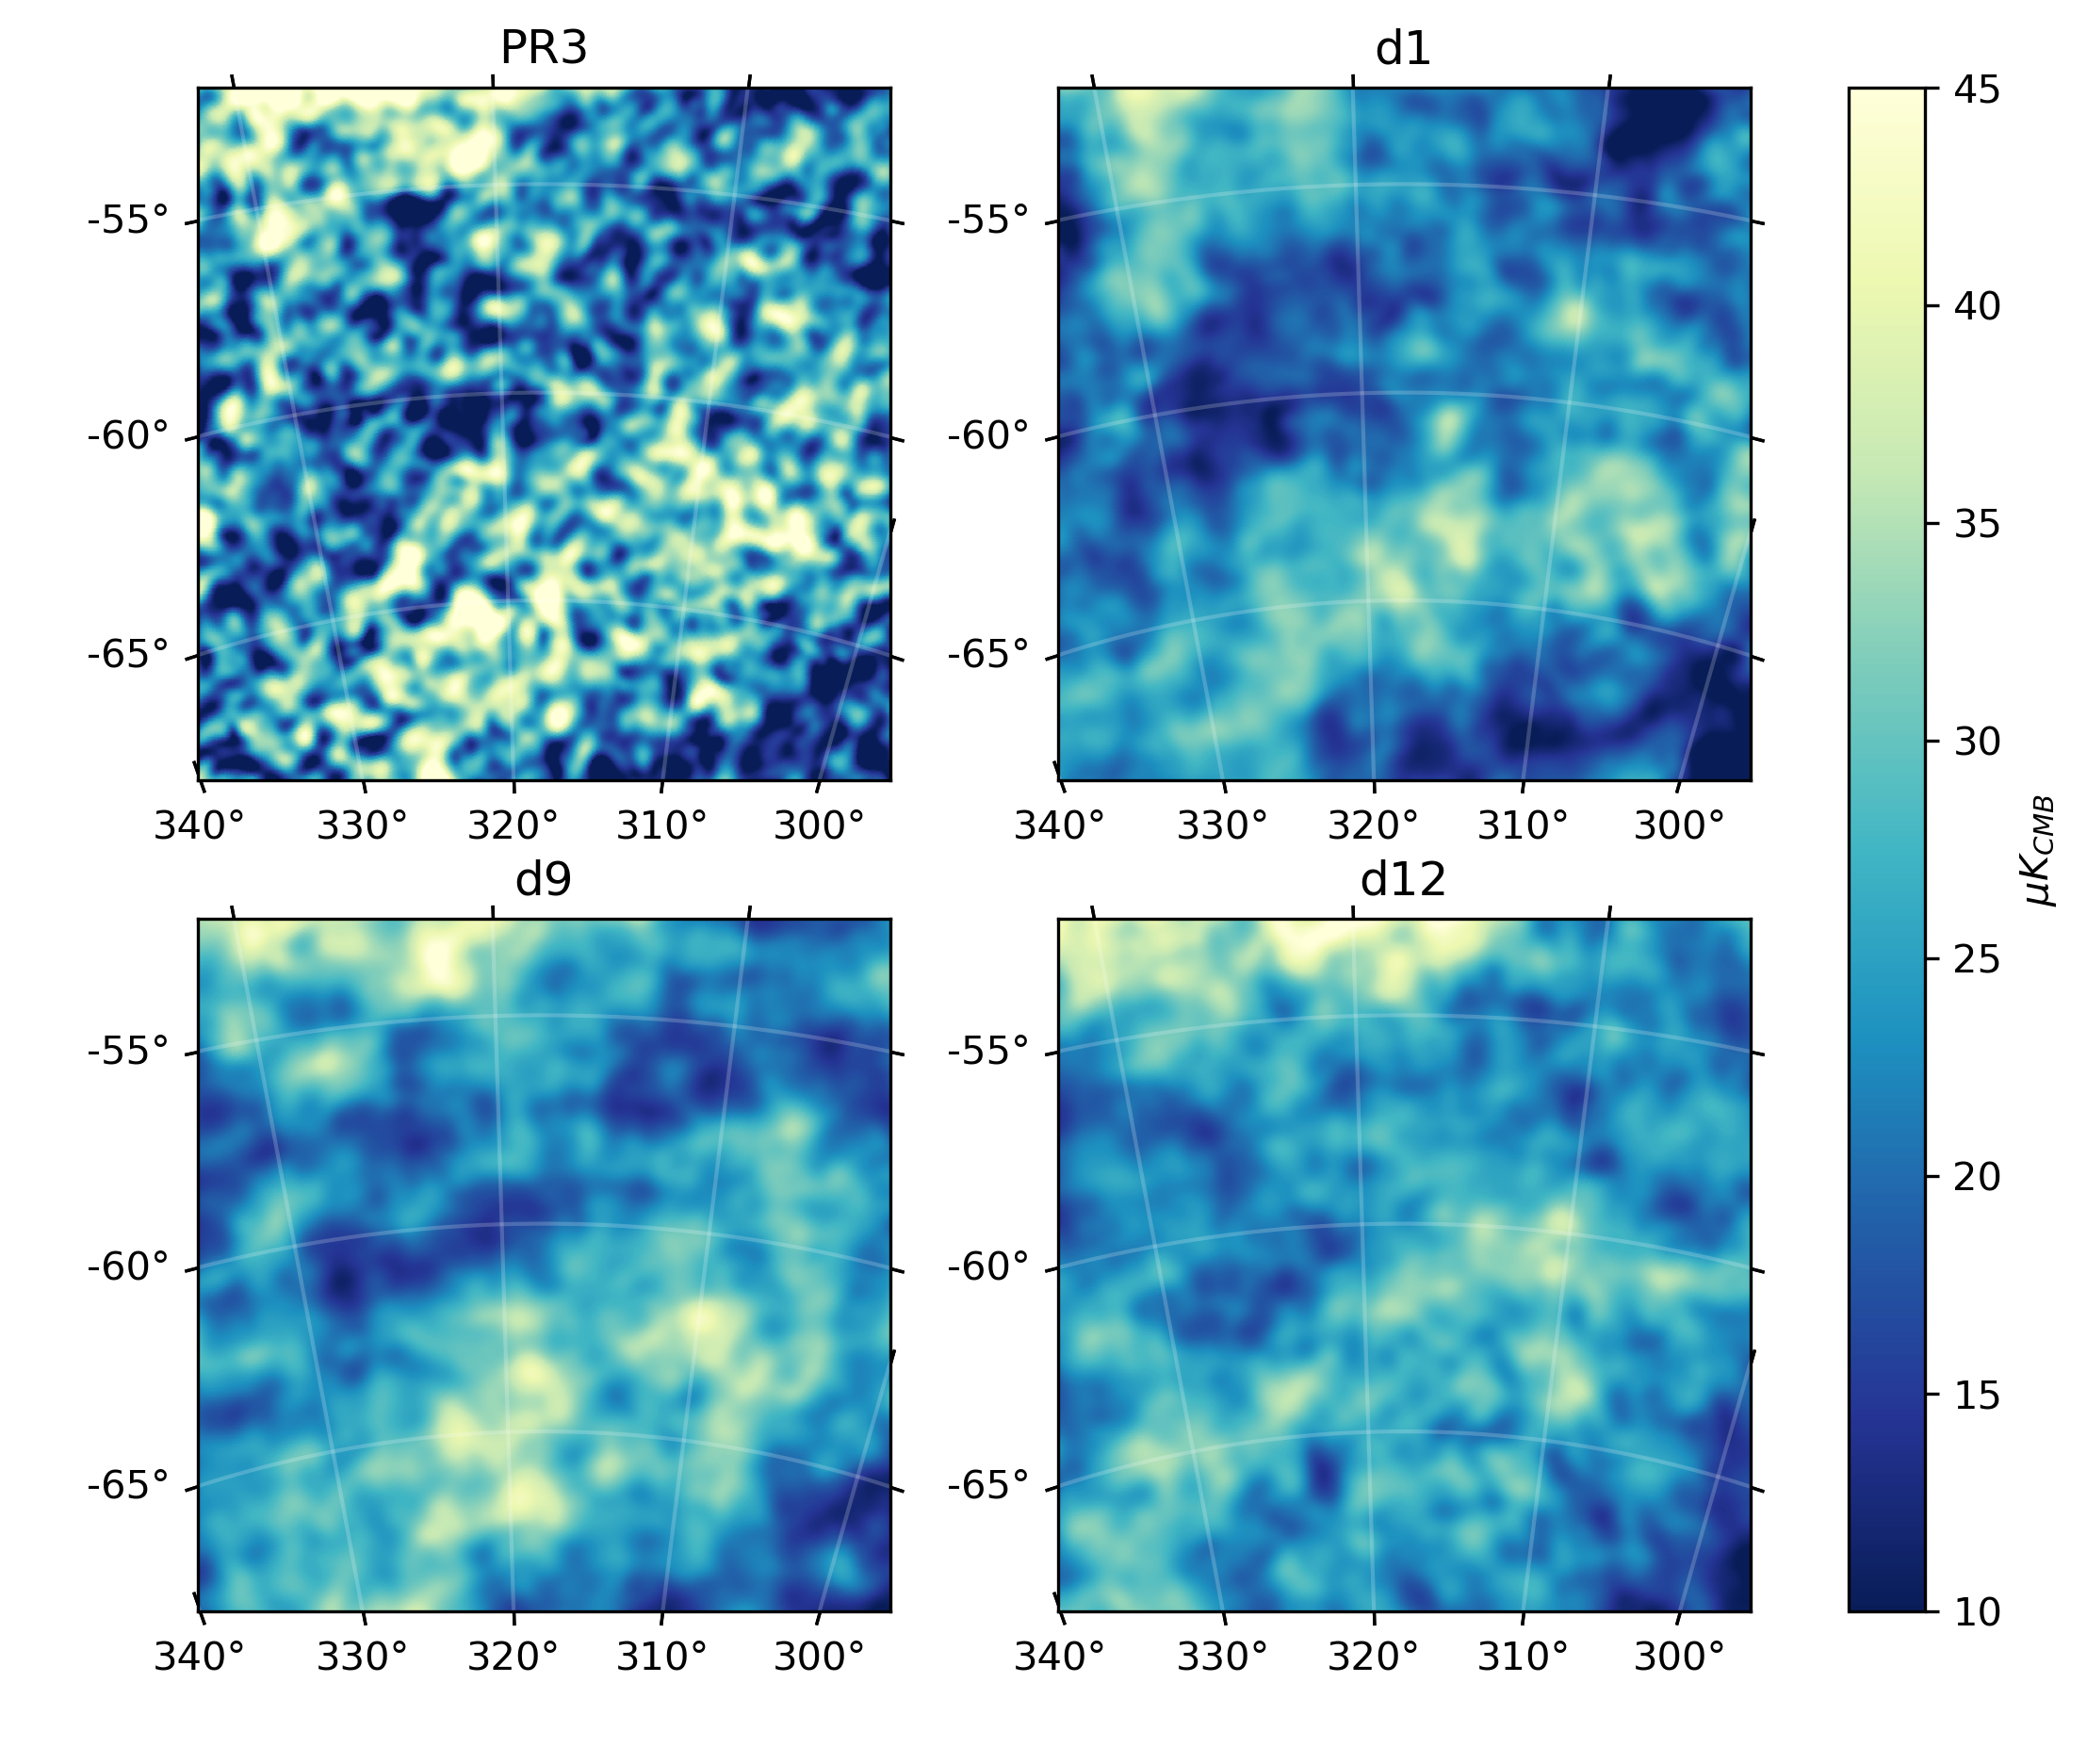
\includegraphics[height=0.41\textwidth]{figures/pol_BK_smooth_30'.png}
    \caption{Polarized dust intensity at 353GHz centered at [l = 180, b = -10] (left) and [l = 318, b = -31] (right), smoothed to $30\arcmin$: (a) PR3 (b) d1 (c) d9 (d) d12.}
    \label{fig:353_pol_int}
\end{figure*}
% \begin{figure}
%     \centering
%     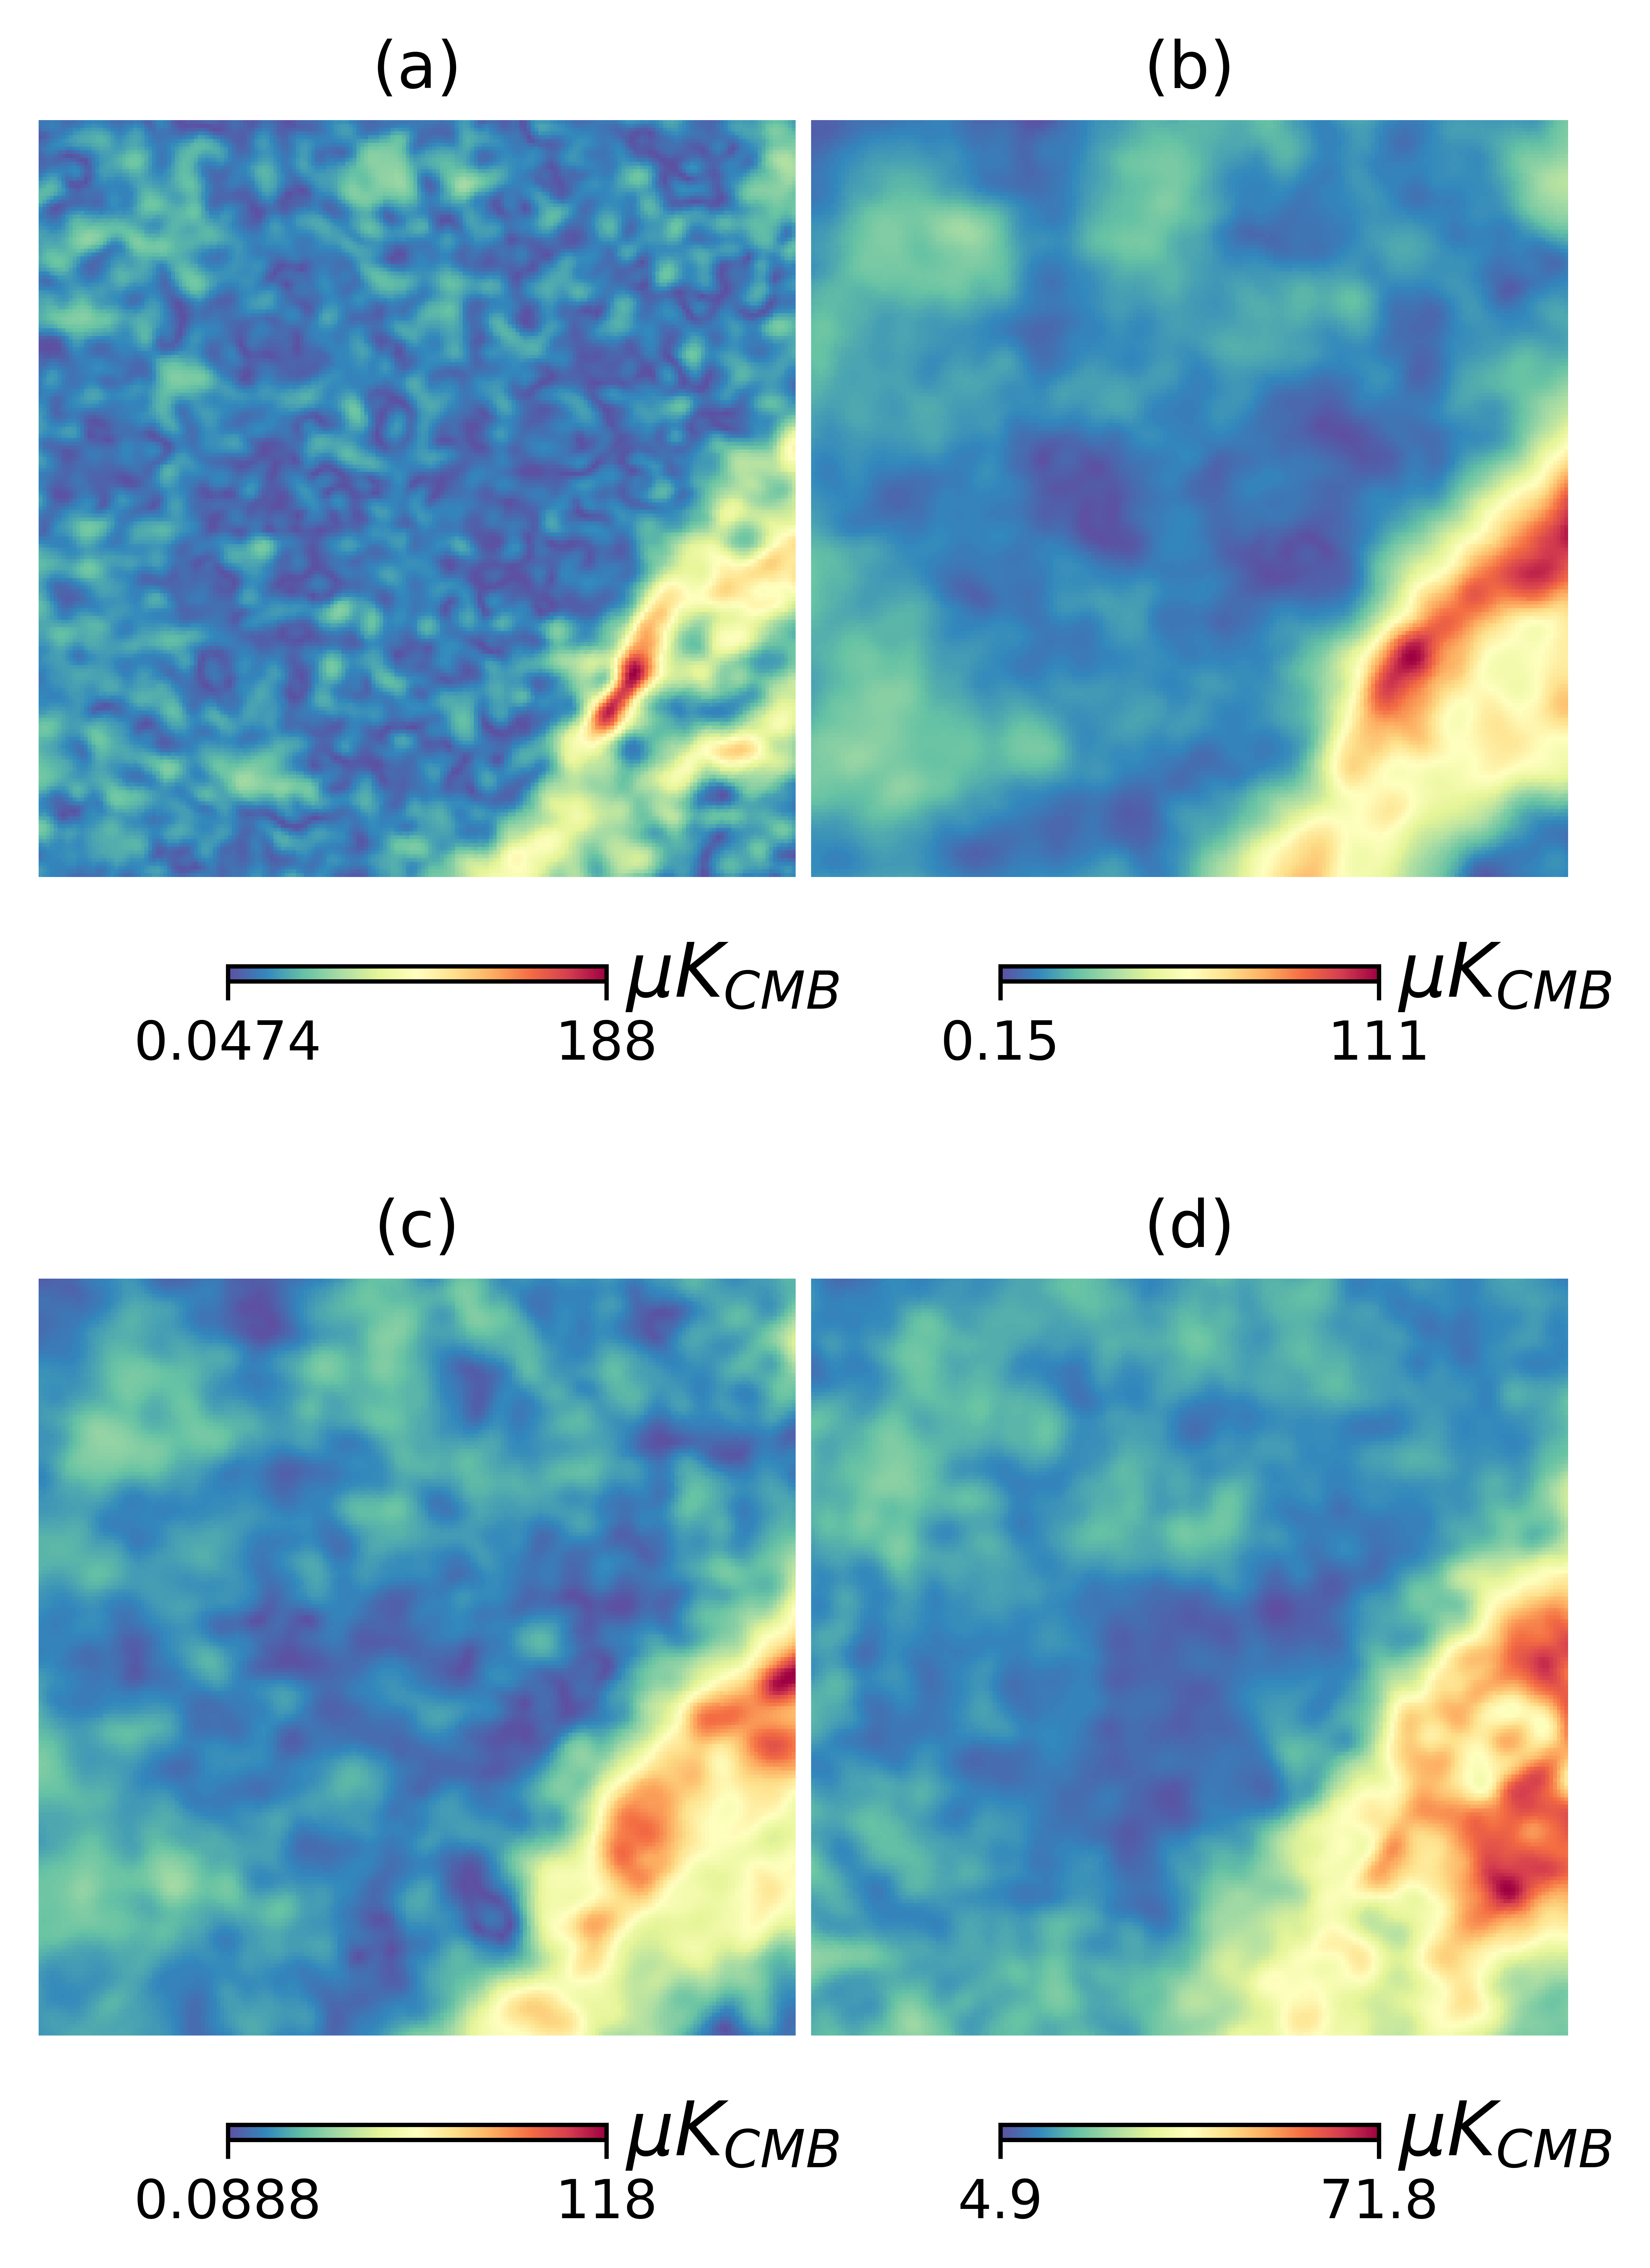
\includegraphics[scale = 0.6]{figures/pol_NGP_smooth_30'.png}
%     \caption{Polarized dust intensity at 353GHz centered at [l = 0, b = 90].}
%     \label{fig:353_pol_int_NGP}
% \end{figure}

% \begin{figure}[ht!]
%     \centering
%     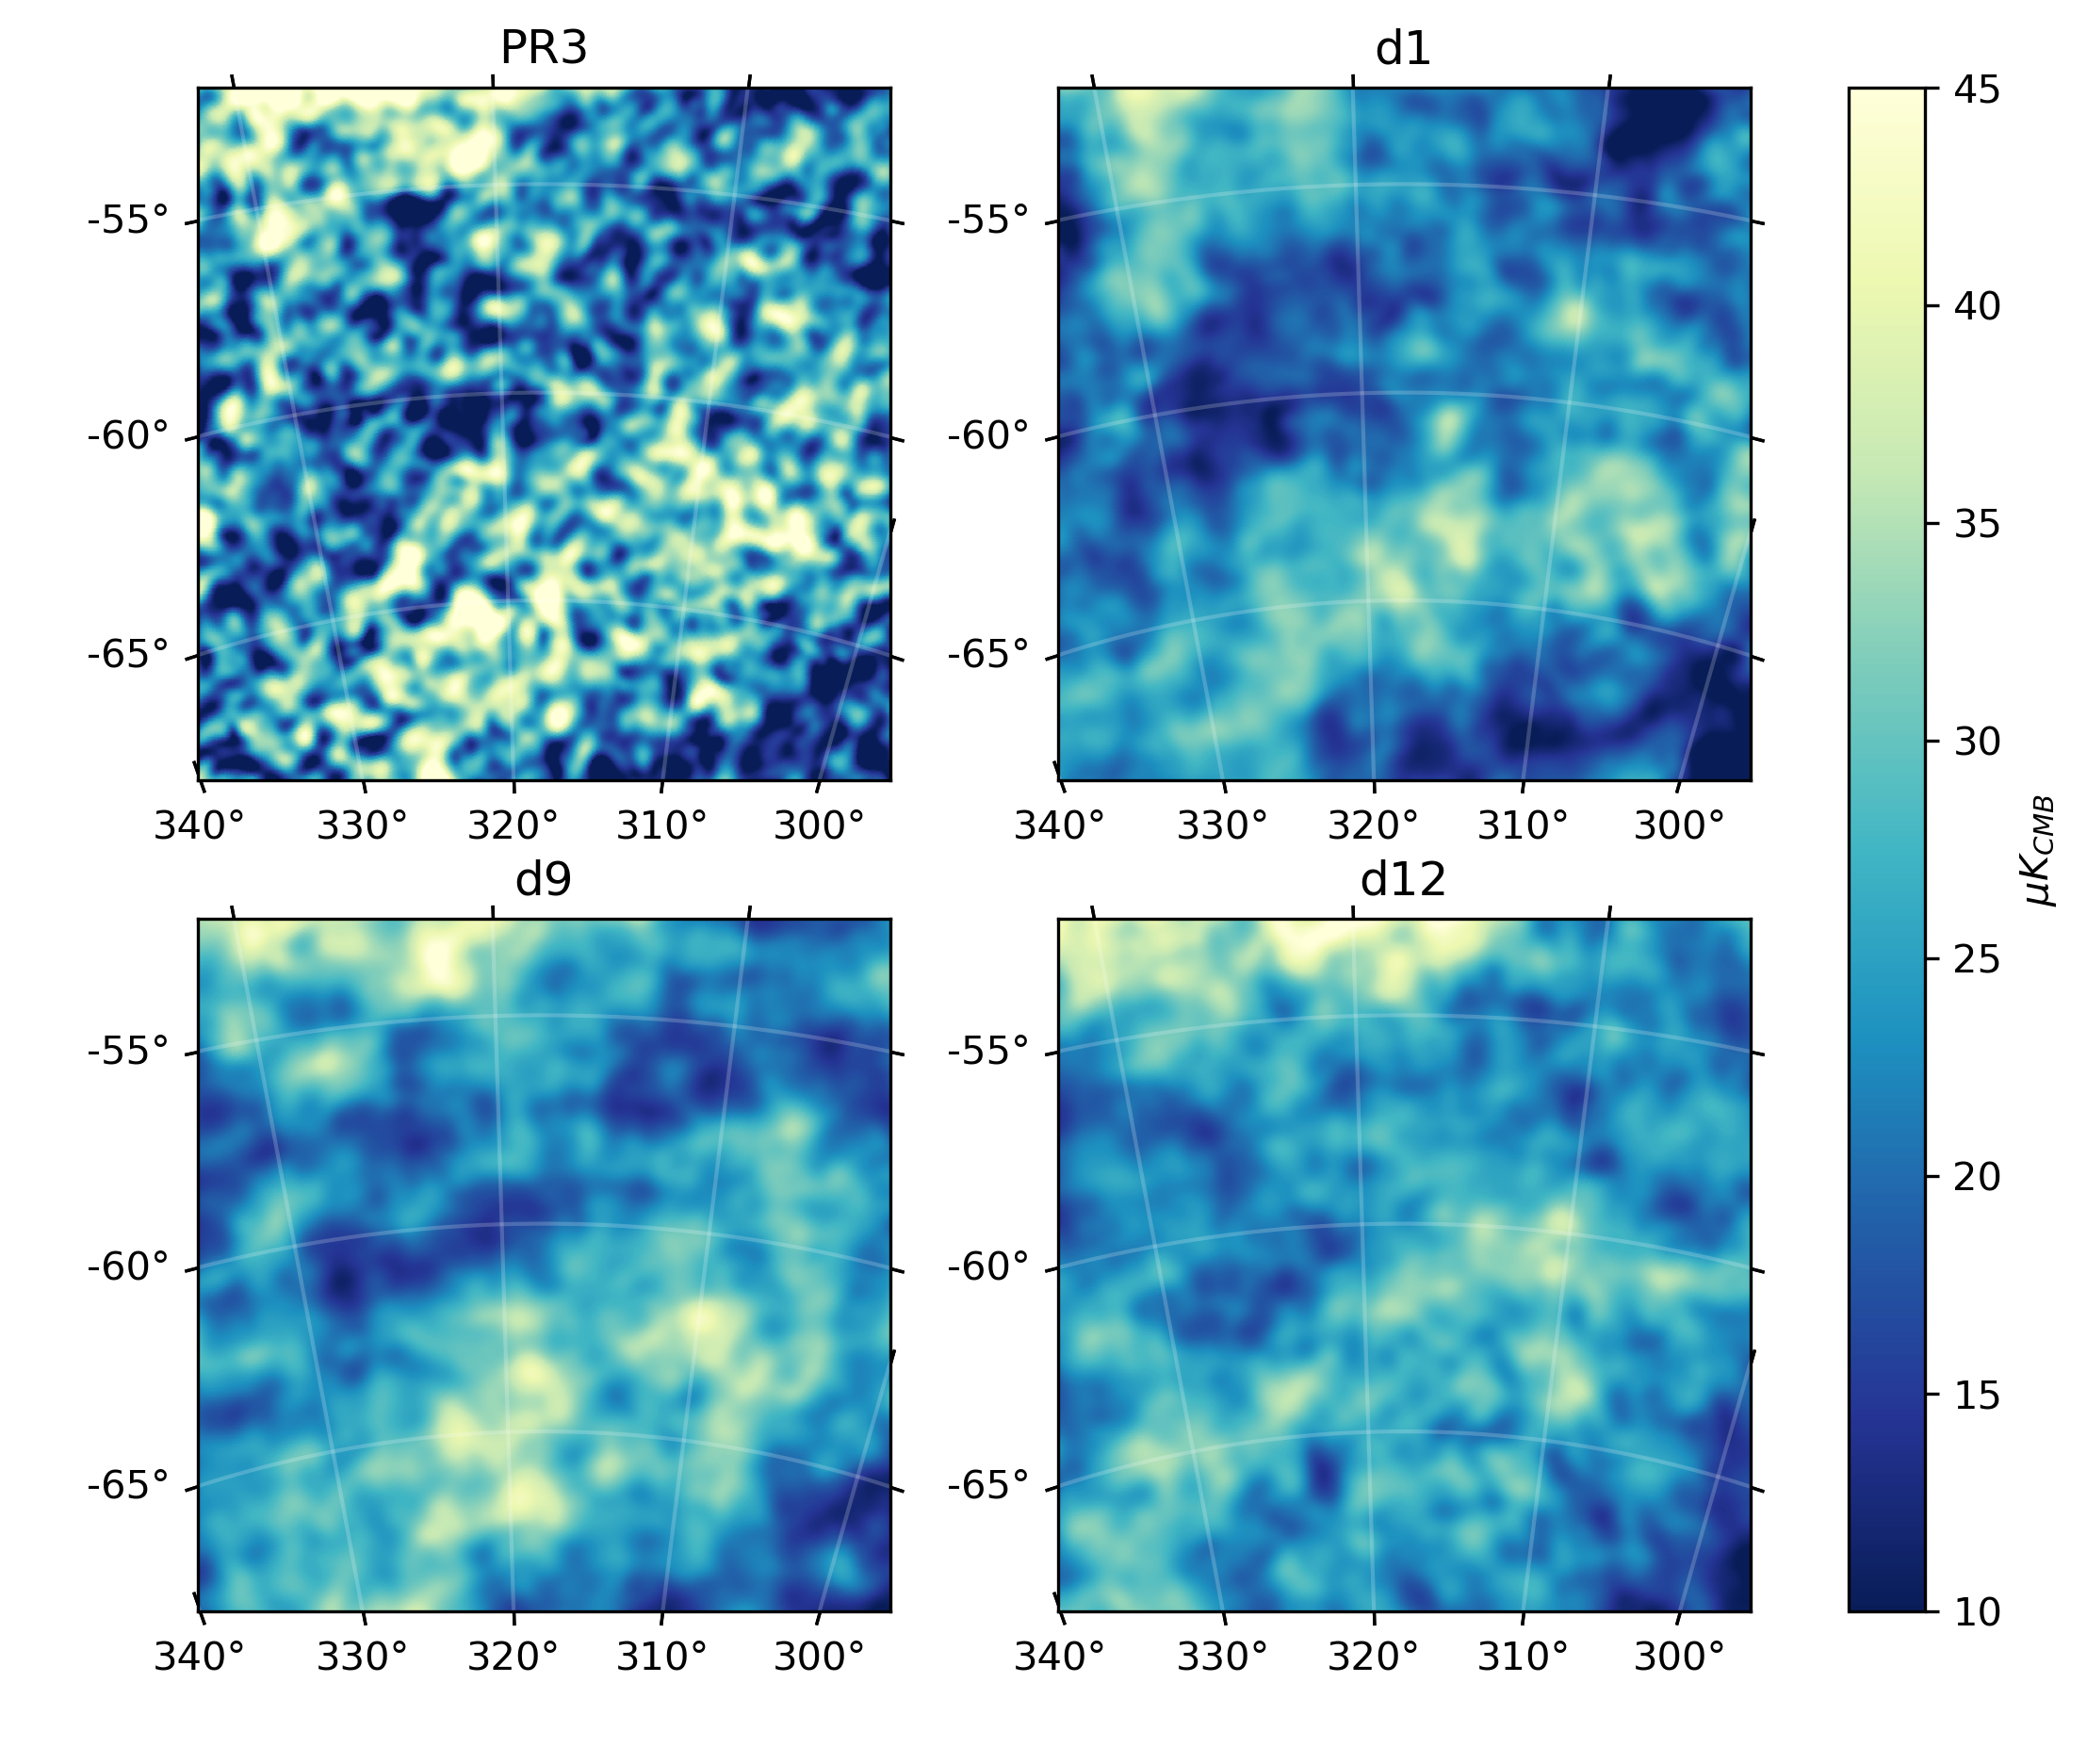
\includegraphics[width=0.5\textwidth]{figures/pol_BK_smooth_30'.png}
%     \caption{Polarized dust intensity at 353GHz centered at [l = 318, b = -61], smoothed to $30\arcmin$: (a) PR3 (b) d1 (c) d9 (d) d12.}
%     \label{fig:353_pol_int_BK}
% \end{figure}

Intensity and polarization at 353~GHz are displayed in Figures~\ref{fig:353_int} and \ref{fig:353_pol_int}. 
%Varying choices for filtering the real data and generation of random small scales result in varying dust emission properties. 
%Jacques
In intensity, model {\tt d9} filters more of the real data and generates more random small-scale structures than models {\tt d1} and {\tt d12}. We can visually appreciate the impact of this choice in the left panel of Fig.~\ref{fig:353_int}, near the Galactic plane. At high Galactic latitudes (right panel of Fig.~\ref{fig:353_int}), the PR3 observations are visibly contaminated by CIB fluctuations, which also contaminate model {\tt d1}. For model {\tt d9}, these CIB fluctuations are replaced by randomly generated small scales. Model {\tt d12}, which uses a 5 arcminute GNILC intensity map \ref{sec:layers}, preserves more of the real dust structures, while filtering much of the CIB contamination.

%As expected, in intensity, we see that d12 is more similar to the actual data in Figure~\ref{fig:353_int} than d9 that has random small-scale generation up to larger scales. We can visually appreciate the impact of different prescriptions for adding small scales in intensity, with more small-scale structures in model d9. 

In Figure~\ref{fig:353_pol_int}, we compare the observations and models for polarized intensity at a resolution of 30' since the PR3 data is contaminated by instrumental noise. 
%In total intensity, d9 and d11 are very similar (with small differences due to the fact that different seeds are used to generate small-scale structures). Real structures are replaced by random realizations as described in section \ref{sec:small_scales}, while for intensity d12 is more similar to the actual data by construction at small scales, and more filamentary. 
% Around the BICEP/Keck patch center (Figure~\ref{fig:353_int_BK}), the PR3 data are contaminated by the CIB, which masks out dust emission. 
Both close to the Galactic plane and in the center of the Bicep/Keck patch, all three models are in reasonable visual agreement with the observations. 
%After smoothing with a Gaussian beam of 30 arcmin, we discern dust structures.

\subsection{Power spectra}
\label{sec:PS-validation}
In this section we discuss the power spectra validation of the PySM dust and synchrotron models. 

\subsubsection{Methodology}
For our large-area validation we employ sky masks that leave 80\%, 60\%, 40\% and 20\% of the sky unmasked. The mask choices for the dust and synchrotron validations are different, as the features of the two emissions are somewhat different. The masking choices are discussed in detail in the individual sections. We use the healpy \texttt{anafast} function to compute power spectra after masking and divide the computed power spectra by $f_{\rm sky}$ (defined as the second moment of the mask) to account for the masking. We make no further attempts to correct for mode-mixing effects due to masking. Methods that correct for mode-mixing due to masking make the explicit assumption that the field is free from any inherent mode-coupling \citep[e.g.,][]{Hivon:2002}. While this assumption is true for the CMB, it is not true for Galactic emission, which is highly non-stationary in nature. We bin the power spectra in dynamic $\ell$-intervals optimized for map noise and sky fraction. Throughout this work we present $\mathcal{D}_\ell \equiv \ell(\ell + 1) C_\ell / 2\pi$, where $C_\ell$ is the power spectrum. All power spectra results in this section are in $\mu{\rm K_{CMB}}^2$ units. %One should assume appropriate unit conversion for observational data or emission models where necessary.

The polarized dust emission is the dominant foreground contaminant for CMB $B$-mode observations. We therefore perform additional validation of the dust $B$-mode polarization in small patches to check the properties of the injected small scales. 

\subsubsection{Dust Emission Over the Sky} \label{sec:dust_validation}
To compare the performance of the latest PySM dust models \texttt{d9}, \texttt{d10} and \texttt{d12} with real data over a broad range of scales, we present their power spectra computed with both large-area and small-area masks at 353~GHz where the dust emission dominates. We first generate PySM dust models maps at delta 353~GHz and smooth them with a Gaussian beam of 4.82\arcmin, matching the resolution of Planck 353~GHz channel. We color-correct the Planck NPIPE 353~GHz channel maps to the same single frequency by a scaling factor 0.92, and we subtract the CMB dipole from the NPIPE temperature maps. We then apply identical masks (defined below) to the mean-subtracted PySM dust models and NPIPE ``A''/``B'' detector-split maps. We finally compute the auto-spectra of the model maps and the cross-spectra of the NPIPE data splits with the masks to minimize noise correlation. 

For our large-area comparison, we use a set of $2^\circ$-apodized Galactic masks\footnote{\texttt{HFI\_Mask\_GalPlane-apo2\_2048\_R2.00.fits}} from the Planck Legacy Archive. There are eight masks in total, leaving between 20\% and 99\% of the sky available. We take \texttt{GAL020}, \texttt{GAL040}, \texttt{GAL060} and \texttt{GAL080} as representative for our analysis, where the number in the mask name indicates the percentage of the sky left for analysis, i.e., $100 f_{\rm sky}$.

In Figure~\ref{fig:largefield_power}, we compare the $TT$, $EE$, and $BB$ power spectra of the \texttt{d9} model, the \texttt{d12} model, and the NPIPE map. Since the \texttt{d10} model is identical to the \texttt{d9} model at 353~GHz, we do not show it separately. The error bars on the cross-spectra are computed from 200 NPIPE detector-split simulations.

For the $TT$ spectra, we find that the \texttt{d12} model aligns well with the observed $TT$ spectrum for all sky fractions, except that it underestimates the power spectrum amplitude when $f_{\rm sky} = 0.8$. The \texttt{d9} model shows similar behavior for $\ell \lesssim 100$. Beyond that scale, its power declines more rapidly with $\ell$ at $f_{\rm sky} = 0.6$ and $f_{\rm sky} = 0.8$, and it exhibits a power bump around $\ell \sim 100$ for $f_{\rm sky} = 0.2$.

For polarization, the \texttt{d9} model is generally consistent with the data over all scales and sky fractions for both $EE$ and $BB$. In contrast, \texttt{d12} significantly underestimates both spectra in all scales. This discrepancy can likely be attributed to the fact that this model is constructed using isolatitude masks, while we use the Planck Galactic masks in this comparison. We also note that the NPIPE $BB$ band power rises at high-$\ell$ due to residual noise which dominates in smaller sky patches.

\begin{figure}
    \centering
    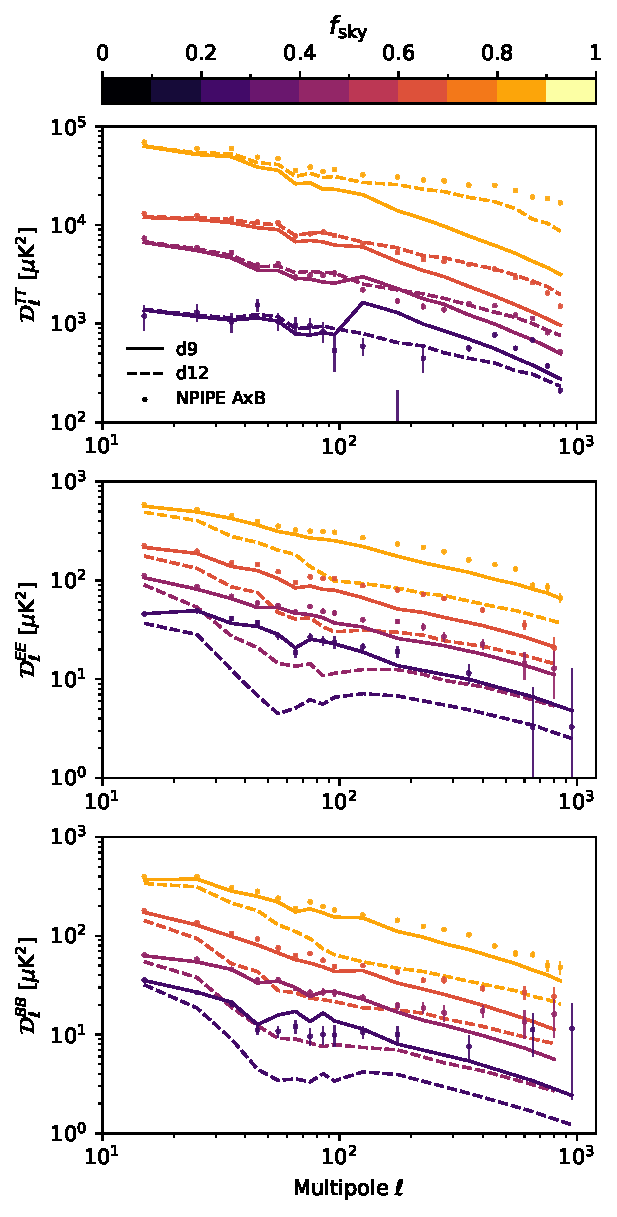
\includegraphics[width=\columnwidth]{figures/largefield_power_all_TEB_pub.pdf}
    \caption{$TT$, $EE$ and $BB$ power spectra of the \texttt{d9} model (solid lines), the \texttt{d12} model (dashed lines) and the NPIPE detector-split maps (circles) when computed on the \texttt{GAL020}, \texttt{GAL040}, \texttt{GAL060} and \texttt{GAL080} Galactic masks. Each set of comparisons is colored in the same color representing their sky fraction $f_{\mathrm{sky}}$. Note that we do not show the \texttt{d10} results as this model is identical to \texttt{d9} at 353~GHz.}
    \label{fig:largefield_power}
\end{figure}

%\begin{figure*}
%    \centering
%    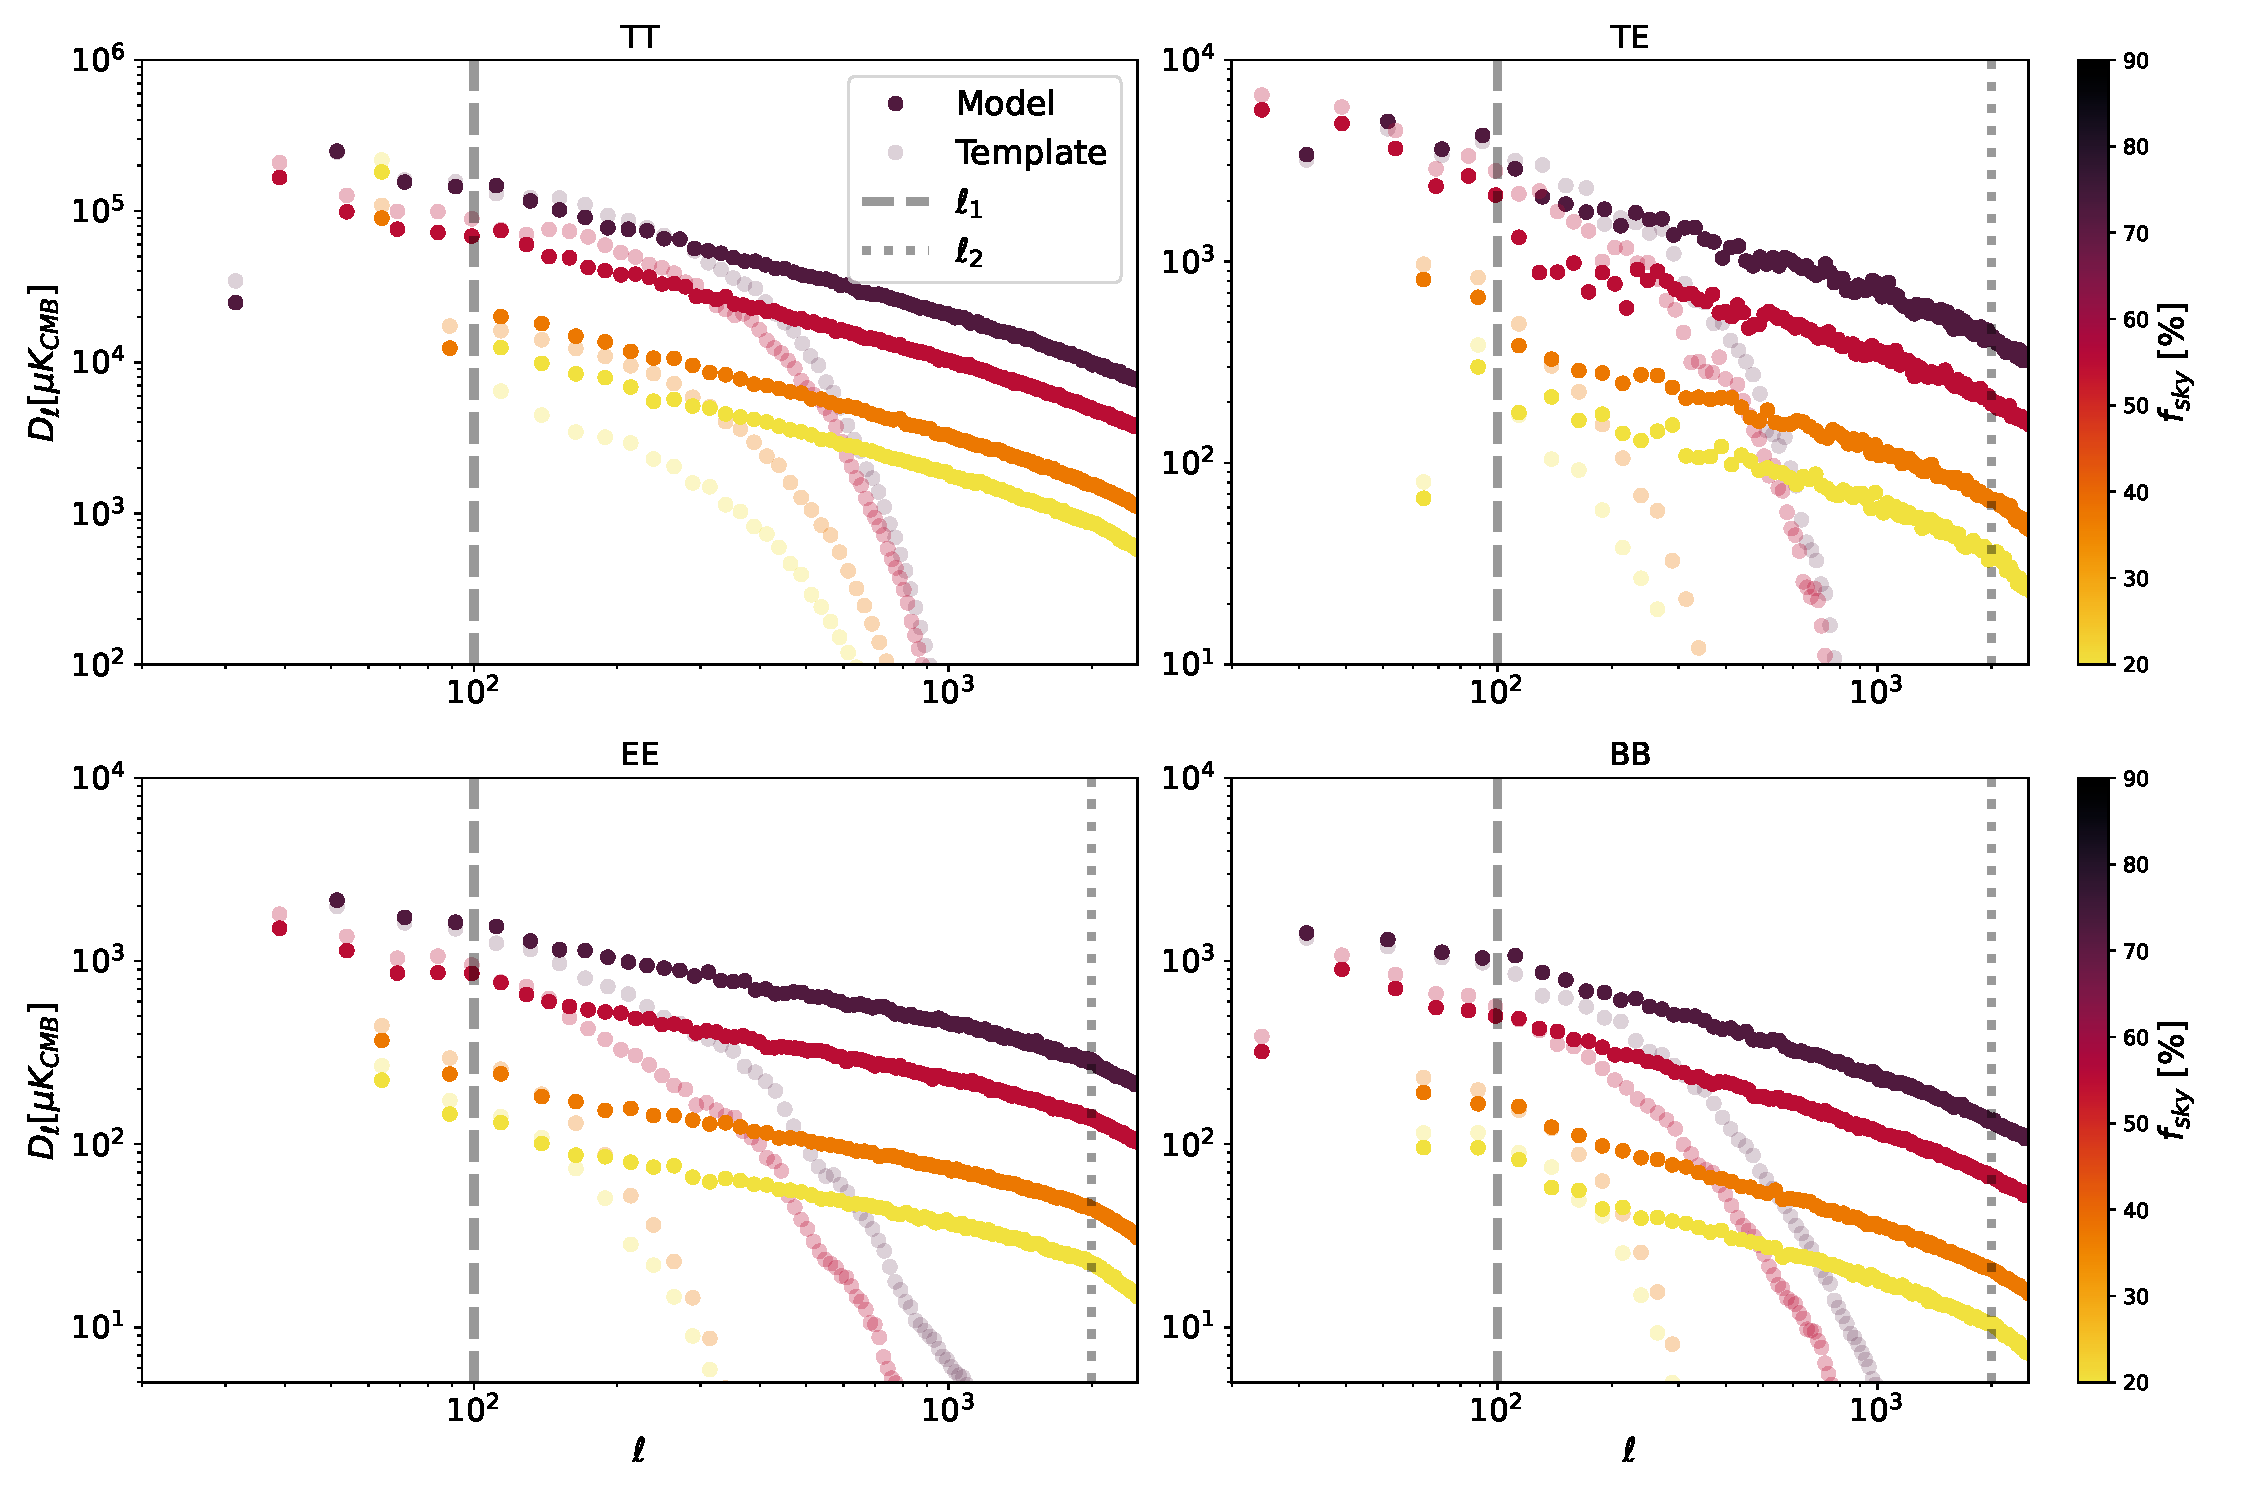
\includegraphics[width=2.\columnwidth]{figures/dust_valspectra.pdf}
%    \caption{This figure compares the power spectra of the \dnine{} model (dark circles) and the input GNILC map (light circles) when computed on the \texttt{GAL090}, \texttt{GAL070}, \texttt{GAL040}, and \texttt{GAL020} Galactic masks.}
%    \label{fig:spectra_by_field}
%\end{figure*}

\begin{figure}
    \centering
    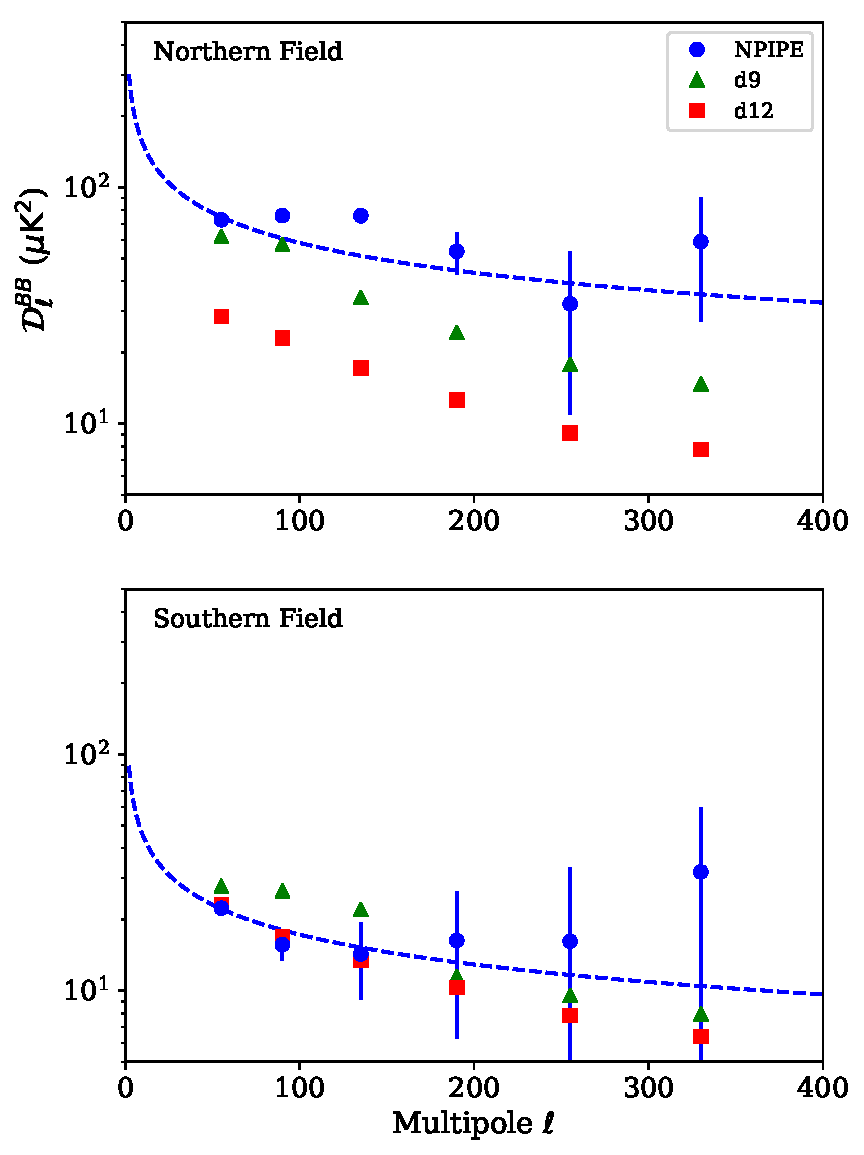
\includegraphics[width=0.48\textwidth]{figures/smallfield_power.pdf}
    \caption{The binned $BB$ power spectra from the 353~GHz NPIPE detector-split maps and dust model maps \texttt{d9} and \texttt{d12}. The dashed lines indicate the best-fit of the fixed-index power law ($\mathcal{D}_\ell^{BB} = A^{BB} \big( l/80 \big)^{\alpha^{BB}+2}$ where $\alpha^{BB} = -2.42$) to the NPIPE data points, which is largely driven by the first two band powers.}
    \label{fig:smallfield_power}
\end{figure}

In the small-area case, we mainly follow the method described in \cite{planck2014-XXX} to define the masks for spectra computation. We first use a HEALPix grid with $\texttt{nside} = 8$ to divide the full sky into 768 patches. At the center of each patch, we create a 400\,deg$^2$ circular mask with its edge tapered by a $2^\circ$ FWHM Gaussian, resulting in $f_{\rm sky} \sim 0.008$. The representative results from two selected circular fields at Galactic latitude $|b| > 30^\circ$ of the northern and southern Galactic hemispheres are shown in Figure~\ref{fig:smallfield_power}. As it would be computational expensive to use simulations to compute the cross-spectra errors of each small sky patch, in this case they are calculated by the method stated in \cite{Tristram:2005}. 

%To compare the small-scale performances of the latest PySM dust models \texttt{d9}, \texttt{d10} and \texttt{d12} with real data, we mainly follow the analysis method described in \cite{planck2014-XXX} to examine the model behaviors. We first use a HEALPix grid with $\texttt{nside} = 8$ to divide the full sky into 768 patches. At the center of each patch, we create a 400-square-degree circular mask with its edge tapered by a $2^\circ$ FWHM Gaussian (resulting in $f_{\rm sky} \approx 0.008$), and apply such a mask to the mean-subtracted dust model and NPIPE half-ring split maps at 353~GHz. We then use \texttt{anafast} to compute the $BB$ auto-spectra of the masked model maps at bin centers $\ell = 55,90,135,190,255,330$ with a dynamic top-hat binning $\Delta \ell = 30,40,50,60,70,80$, and scale them to be the full-sky $\mathcal{D}_\ell^{BB}$, accounting properly for the $f_{\mathrm{sky}}$ of the circular mask. For the masked NPIPE data maps, we instead compute cross-spectrum from the two split maps to minimize the noise correlation. The representative results from two selected circular fields at $|b| > 30^\circ$ of the northern and southern Galactic hemispheres are shown in Fig.~\ref{fig:smallfield_power}. 

\begin{figure}
    \centering
    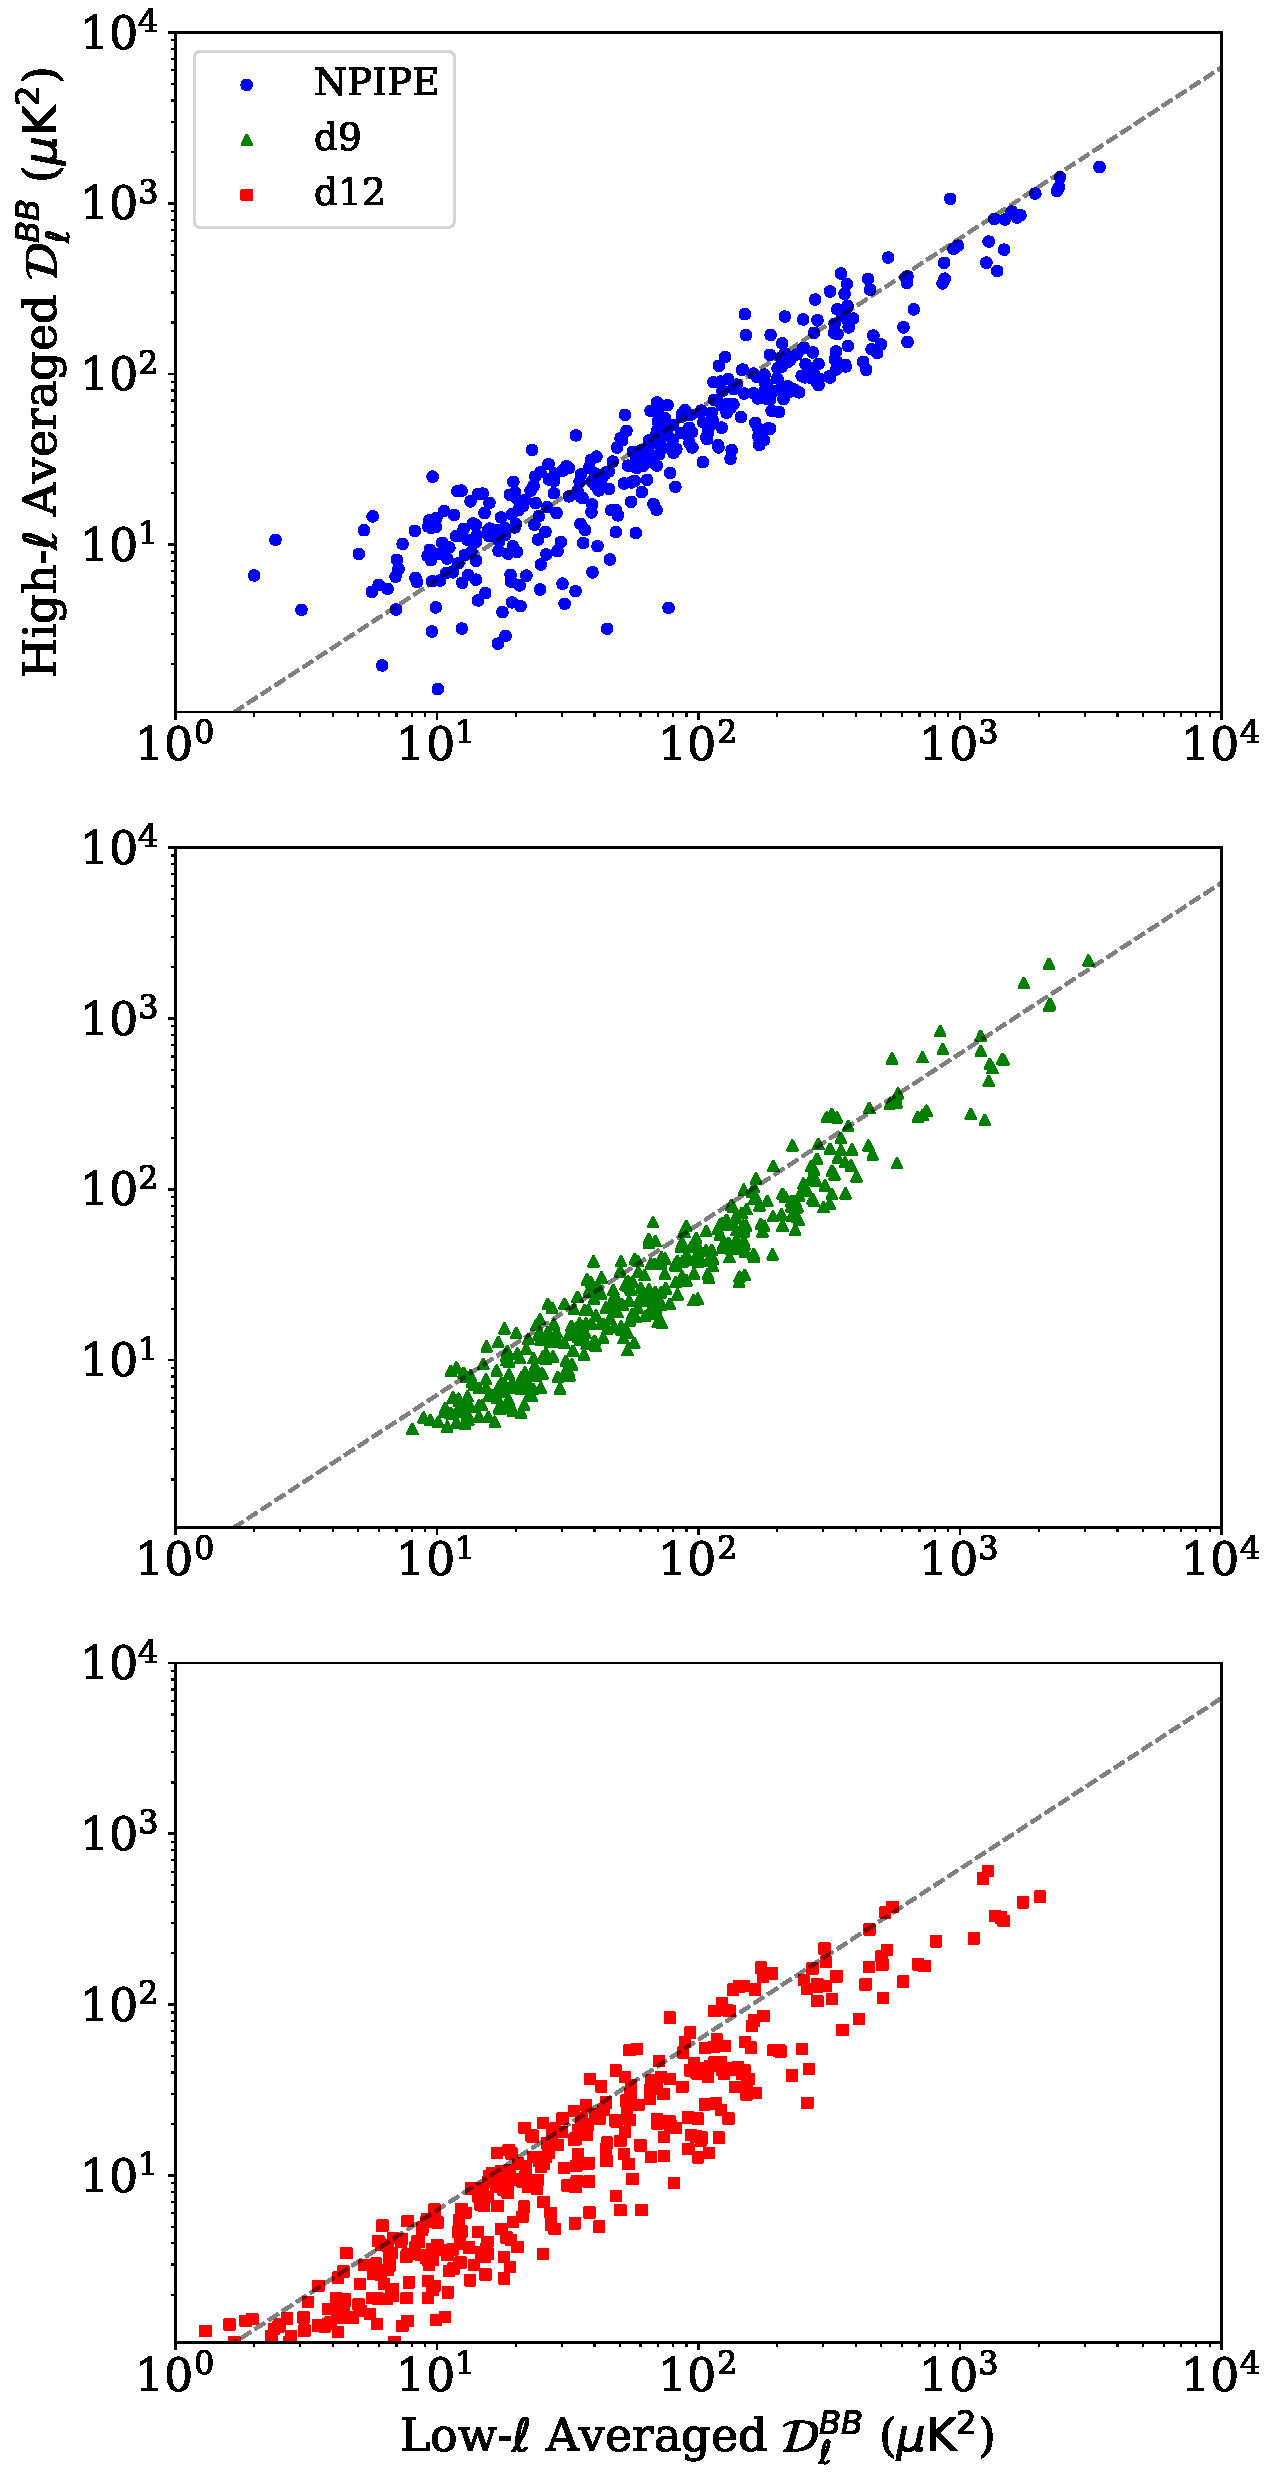
\includegraphics[width=0.48\textwidth]{figures/all2_lhmean.pdf}
    \caption{Scatter plots of the mean of the first two $BB$ band powers versus the mean of the last four $BB$ band powers shown in Figure~\ref{fig:smallfield_power}. Each data point represents the results from a circular sky patches with $|b| > 30^\circ$. Dashed reference lines indicating $\mathcal{D}_\ell^{BB} \propto \ell^{-0.42}$ are added to the plots. This power law in fact comes from the analysis of several larger sky regions ($f_\text{sky} = 0.3 \; \text{to} \; 0.8$) by \cite{planck2014-XXX}, but the small-field NPIPE data points, which spread out when the dust amplitude is small presumably due to map noise, are consistent with it as well. Another important feature is that the trends of the \texttt{d9} and \texttt{d12} data points are lower than that of the NPIPE in these log-log plots, implying that the model spectra are steeper.}
    \label{fig:smallfield_power_all}
\end{figure}

We explore whether the PySM models can reproduce the observed dust $BB$ power spectrum's amplitude, and scaling-in-$\ell$, especially in those high Galactic latitude small fields which could be part of future CMB observations. We therefore compute the low-$\ell$ averaged $\mathcal{D}_\ell^{BB}$ (over $40 \le \ell < 110$) and the high-$\ell$ averaged $\mathcal{D}_\ell^{BB}$ (over $110 \le \ell < 370$) of each small field for the model and NPIPE maps, and we present the results as scatter plots in Figure~\ref{fig:smallfield_power_all}. We define the ratio of the low-$\ell$ mean value (plotted on the x-axis) to the high-$\ell$ mean value (plotted on the y-axis) as a proxy for describing the spatial power change across the modulation scale. The perfect fixed-index power law $\mathcal{D}_\ell^{BB} \propto \ell^{-0.42}$ yields a value of $\sim 1.60$ for this ratio, the NPIPE maps give $1.86 \pm 0.93$ and the \texttt{d9} (\texttt{d12}) model map gives $2.37 \pm 0.77$ ($2.24 \pm 0.87$) over sky patches with $|b| > 30^\circ$.

The amplitude of the \texttt{d12} model is in general smaller than observed in the NPIPE data, as a large fraction of the \texttt{d12} data points cluster around the lower-left corner of the plot. The wider span of the \texttt{d12} data points along the vertical direction also implies the model spectrum steepness varies more over the sky. In contrast, the \texttt{d9} data points are fairly compatible with those from NPIPE maps, although they have slightly steeper power spectra.

\subsubsection{Synchrotron Emission Over the Sky} \label{sec:sync_validation}

In this section, we detail the validation of the new synchrotron models by comparing the power spectra with observations. For validating the PySM synchrotron temperature models, we use the synchrotron map\footnote{\url{https://beyondplanck.science/products/files\_v1}} from the BeyondPlanck re-analysis of Planck LFI data \citep{Andersen:2023}. This map is at a reference frequency of 30\,GHz and has an angular resolution of $2^\circ$. We produce single-frequency temperature maps for the different synchrotron models at 30\,GHz and smooth with a Gaussian beam with FWHM = $2^\circ$.

\begin{figure}
    \centering
    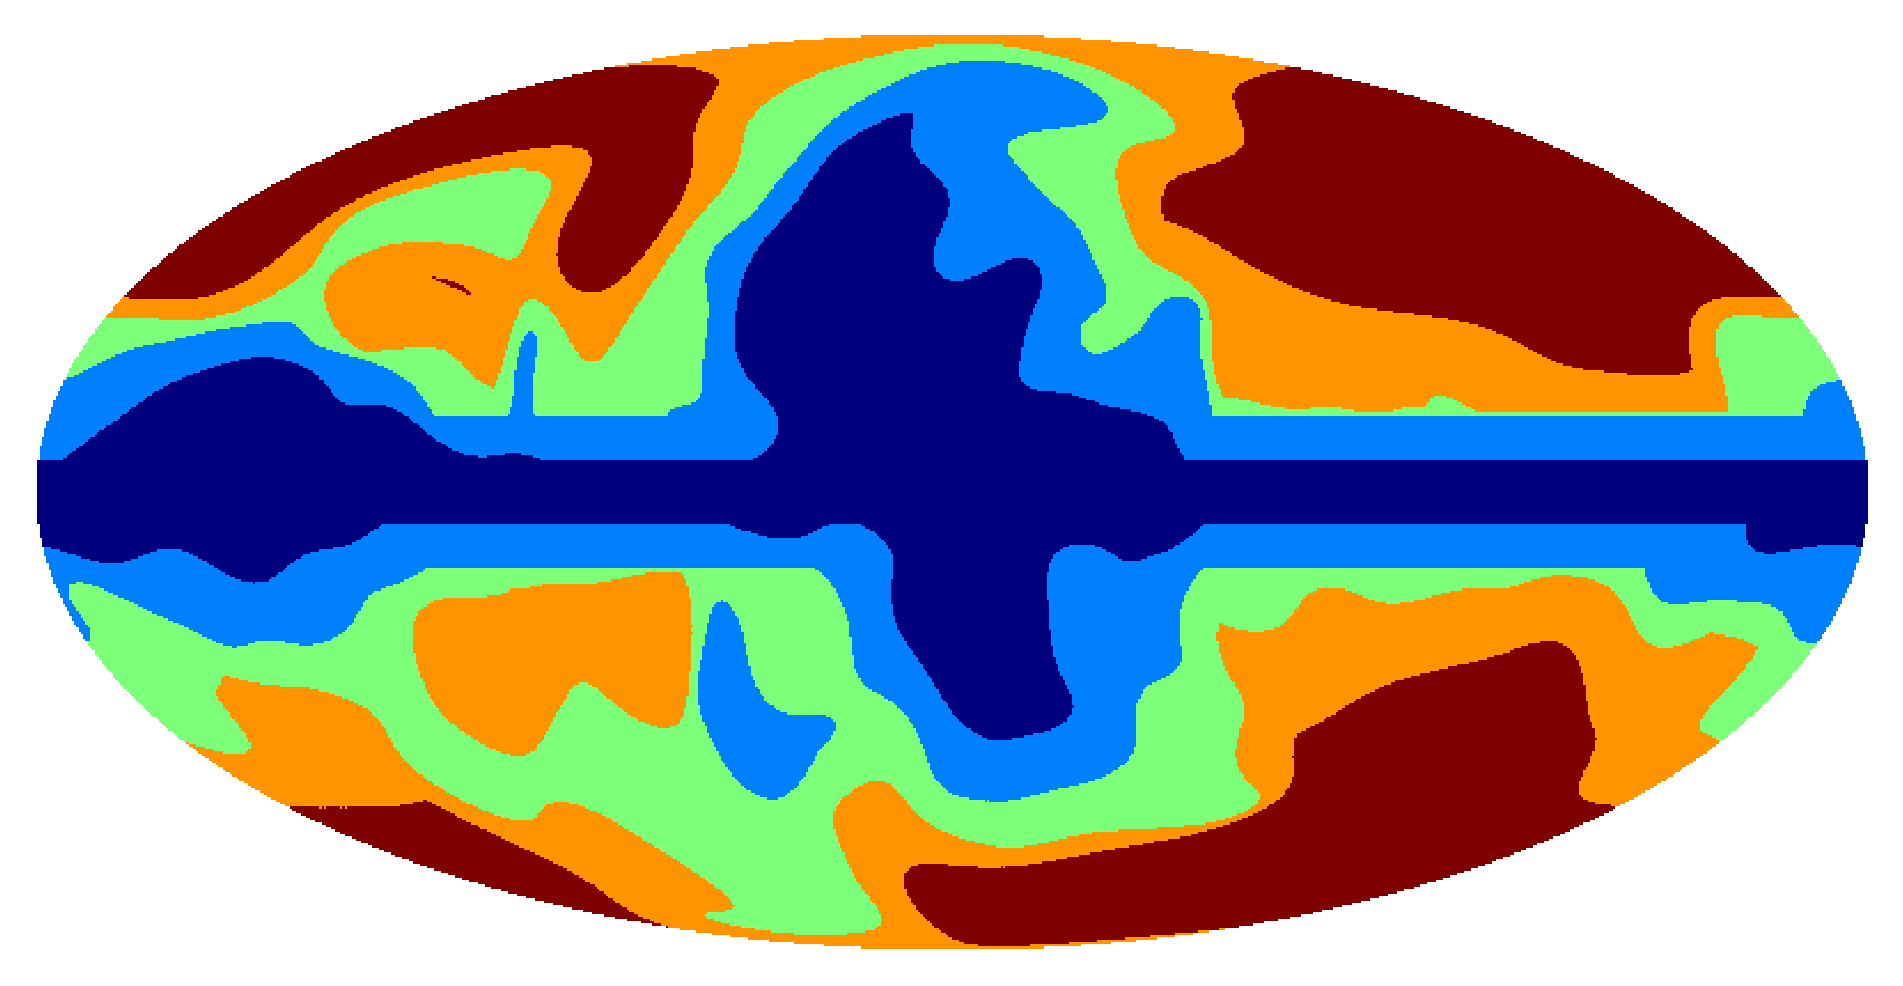
\includegraphics[width=0.46\textwidth]{figures/SYNC_mask_stack.png}
    \caption{Figure showing the four different Galactic masks used for the synchrotron validation. The red region is the 20 \% mask; the orange region shows the additional sky coverage for 40 \% mask; the yellow region shows the added coverage for 60 \%; the green region is the added sky patch of 80 \% mask. The purple region is excluded in all masks. }
    \label{fig:sync_masks}
\end{figure}

We have purposefully chosen an earlier release of BeyondPlanck for our analysis. Later versions of BeyondPlanck, or its successor, CosmoGlobe produce synchrotron intensity maps at 408\,MHz. The PySM synchrotron models s5 and s7 are not suitable for producing synchrotron simulations at 408 MHz. This is a consequence of scaling the Haslam map from 408\,GHz to 30\,GHz for constructing the template for synchrotron intensity. When this template is rescaled to 408\,MHz, with scaling that varies over the the sky, the model fails. We do not recommend use of the s5 and s7 models below 1\,GHz. Therefore, we validate our models with the synchrotron intensity map at 30\,GHz.

% \giuse{In case of the synchrotron polarization, we  compare the models with band integrated observations. So, we compute bandpass integrated maps  with PySM~3 routines and for  the different synchrotron models. For the sake of fair comparison with Planck data, we adopt the average LFI 30\,GHz RIMO transmission \citep{planck2014-a03}.} The bandpass integrated maps are further smoothed with Gaussian beams of 33.1\arcmin beams to produce model maps at native resolutions of the LFI 30\,GHz data. Finally, the observed power spectra are computed by taking the cross-spectrum between independent detector splits, e.g. A and B, of the NPIPE \footnote{Publicly available through NERSC at \\ /global/cfs/cdirs/cmb/data/planck2020} (PR4) 30\,GHz maps \citep{planck2020-LVII}. 

For synchrotron polarization validation, we compare the models with Planck Revisited synchrotron polarization maps\footnote{\url{https://portal.nersc.gov/project/cmb/Planck\_Revisited}} \citep{Delabrouille:2024}. These are the cleanest full sky maps of polarized synchrotron at 30\,GHz at $1^\circ$ resolution at the time of analysis. 
% We convert the Planck Revisited synchrotron maps from $\mu {\rm K_{RJ}}$ to $\mu {\rm K_{CMB}}$. 

We do not use the Planck Galactic masks for the synchrotron power spectra validation. The Planck Galactic masks capture the shape of the Galactic dust signal, as it is the brightest foreground at CMB frequencies. The shape of the Galactic synchrotron signal differs significantly from the shape of the Galactic masks. Therefore, we construct masks for the synchrotron by thresholding the synchrotron polarized intensity smoothed with a $8.5^\circ$ beam. We additionally mask out a portion of the Galactic plane with a narrow band mask. This ensures that we are always excluding the Galactic plane. In Figure~\ref{fig:sync_masks} we show the regions of these masks. 

We also use the Planck Revisited point source mask to mask out the brightest point sources for the polarization analysis. The combined mask is apodized with a $2^\circ$ -- $6^\circ$ cosine taper. The apodization length increases with decreasing sky fraction. We compute the noise bias and standard deviation from 200 noise realizations. The polarization power spectra are corrected for the noise bias. The noise standard deviation represents the error on the power spectra due to noise.

% We use HEALPix \footnote{https://healpix.sourceforge.io} \texttt{anafast} function \citep{Gorski:2005, Zonca:2019}  to compute the power spectra for the model and observation maps,  accounting for the partial sky coverage by dividing by an $f_{\rm sky}$ factor.
% For this validation test, 
%do not use a pseudo-$C_\ell$ estimator as the synchrotron signal is not statistically isotropic, and we correct for the partial sky by naively dividing by an $f_{\rm sky}$ factor.

\begin{figure}
   \centering
   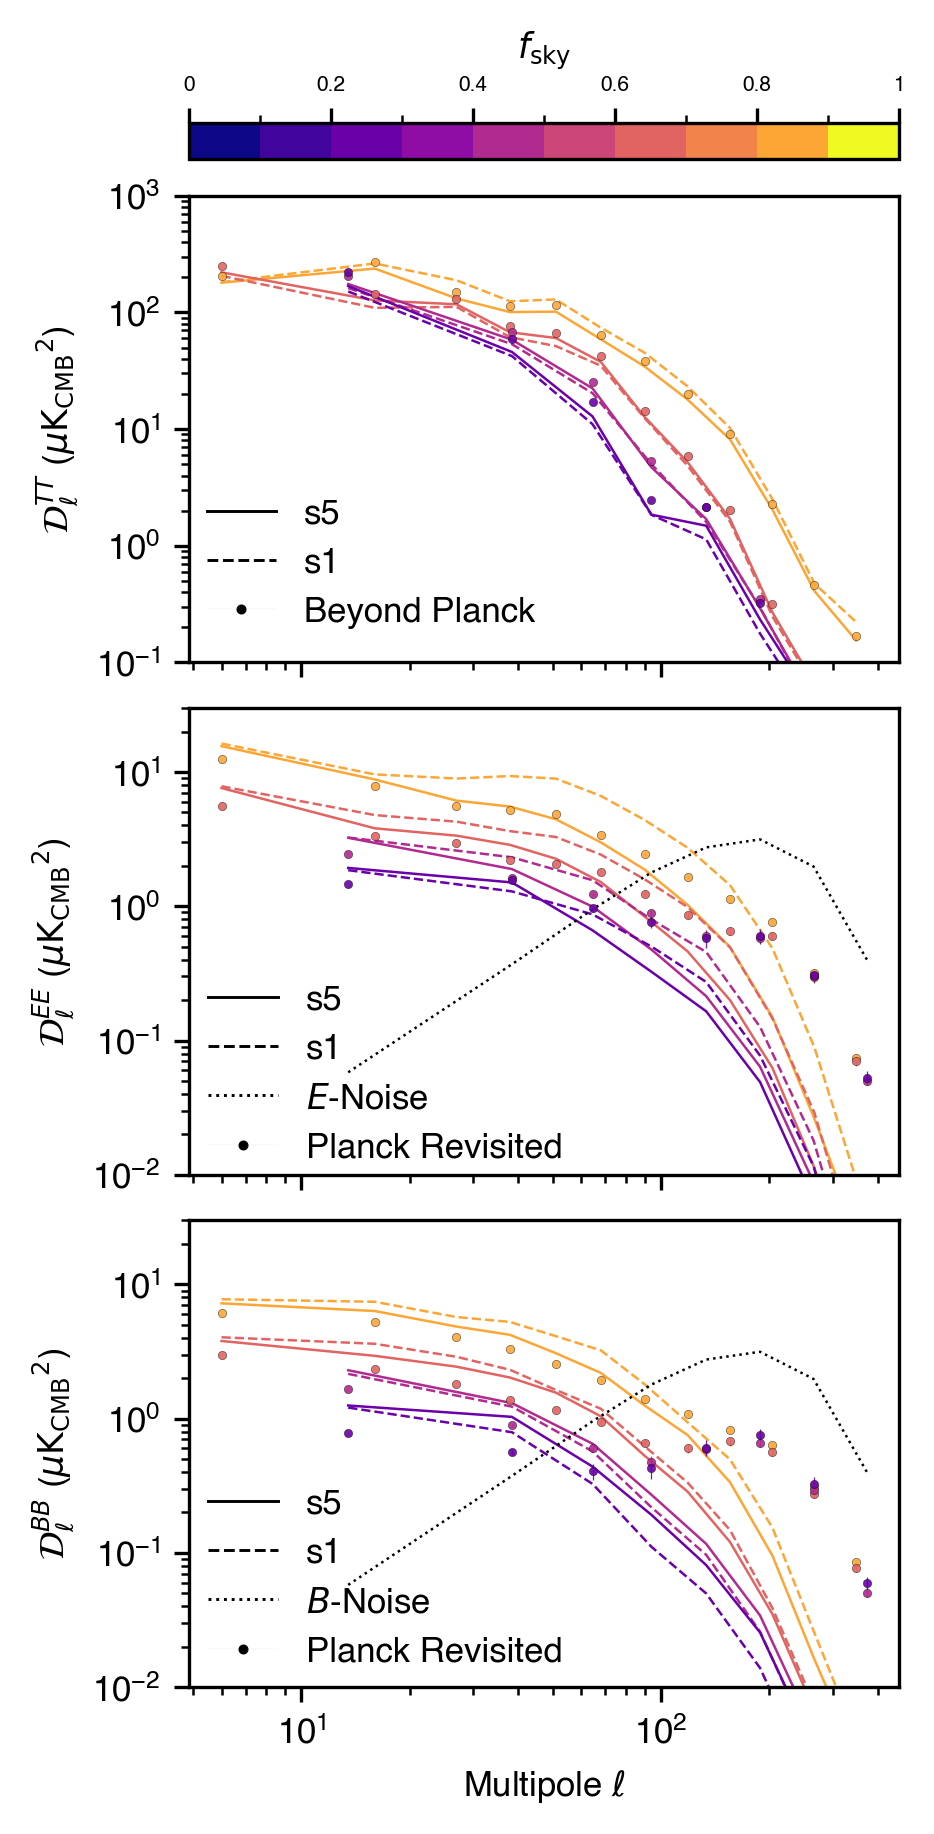
\includegraphics[width=0.48\textwidth]{figures/Dlcomp_PySM3-4_s5_vs_BPPR_SYNC.png}
    \caption{Figure showing comparison of power spectra of the PySM s5 model with observation on different sky fractions. The spectra obtained for models s4, s6 and s7 are similar so we don't show them here. The $TT$ power spectrum comparison is done with synchrotron intensity map from BeyondPlanck release 1 \citep{Andersen:2023} at 30 GHz with $2^\circ$ beam. The $EE$ and $BB$ power spectra are compared with Planck Revisited \citep{Delabrouille:2024} polarized synchrotron map at 30\,GHz with $1^\circ$ beam. The EE and BB spectra for observations are debiased for noise, computed from 200 simulations.}
   \label{fig:Dl_sync_galmask}
\end{figure}

The $TT$, $EE$ and $BB$ power spectra comparisons for model \texttt{s5} are shown in Figure~\ref{fig:Dl_sync_galmask}. The comparison for models \texttt{s4}, \texttt{s6} and \texttt{s7} have nearly identical results, so we only show the results for model \texttt{s5}. The $TT$ power spectra for all sky fractions show excellent agreement with the BeyondPlanck synchrotron temperature power spectra. For polarization $E$ modes, we find a good agreement with observations for all but the 20 \% sky fraction. 
% So, it is reasonable to argue that for synchrotron temperature there is excellent agreement for all but the brightest parts of the sky, where the comparison is harder to make at 30\,GHz. 
For BB spectrum, the PySM model has slightly higher power, for $\ell < 100$. The difference increases at smaller sky fractions. However, such a discrepancy is somewhat expected as we are considering multipoles that are far from the injection scale, $\ell_*\sim36$.
% In fact, some of the features observed in the LFI 30 GHz spectra are not found in the pysm spectra as they are by construction generated to have a power law shape.
For $\ell \sim 200$, we find a bump in spectrum for the Planck Revisited observations. This is probably a combined effect of residual point sources, incorrect masking choice in $B$-mode polarization, and perhaps some residual noise. In particular, we computed the synchrotron masks with smoothed synchrotron polarized intensity maps, to prevent small holes in the mask. However, such masking may not always correctly mask small scale structures. This would result in some bright, partly-clipped objects producing some of the features we see in the observed power spectrum. 

An important caveat of the current synchrotron templates is that despite the point source masking, we find excess power due to Galactic point sources at low  Galactic  latitudes around the Galactic center. Thus, we conclude that the \texttt{s4}, \texttt{s5}, \texttt{s6} and \texttt{s7} models are reliable at $\ell \lesssim 3000$ and outside the Galactic plane. We devote to a future release the treatment of small scale structure in bright regions.


\subsubsection{Dust and Synchrotron Emission in the BICEP/Keck Patch}
\label{sec:BK_validation}
\begin{figure*}
    \centering
    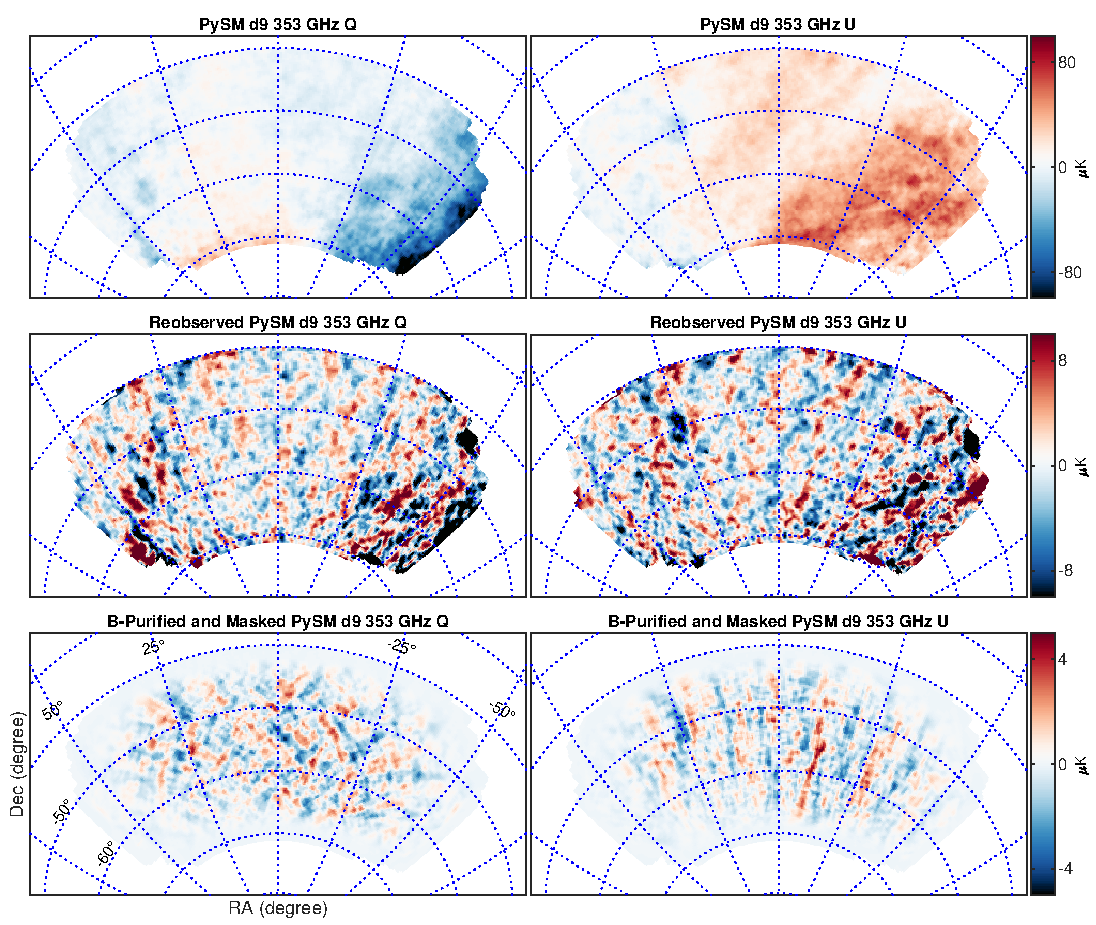
\includegraphics[width=2.\columnwidth]{figures/pysm_d9_353_delta_reobs_B_pub.pdf}
    \caption{The PySM \texttt{d9} maps, reobserved maps and purified maps in the BICEP/Keck sky patch at delta 353 GHz. Each panel shows the
    PySM $Q$/$U$ maps reprocessed by the BK18 BICEP3 beam profile, observation matrix and purification matrix respectively.}
    \label{fig:psym_BKmatrix}
\end{figure*}

The cleanest patch of sky in the southern hemisphere is particularly important for ongoing and future CMB experiments that target the primordial B-mode polarization. The dataset providing the strongest constraining power of the tensor-to-scalar ratio $r$ to date is from the BICEP/Keck (BK) experiment with science data up to the 2018 observation season~\citep[``BK18'';][]{Ade:2021}. It comprises a combination of BK, NPIPE and WMAP 23--353~GHz data observed from the $\sim 600$ square degree sky patch centering at RA 0h, Dec. $-57.5^{\circ}$. Over the next few years, a collaborative effort between the BICEP/Keck and the South Pole Telescope (SPT) will combine the BICEP3 and BICEP Array maps with the overlapping SPT-3G maps in order to ``delens'' the observed CMB B-modes to tighten the constraint on $r$~\citep{BICEP/KeckCollaboration:2022}. As this observation field will also overlap with the tentative sky patch of the CMB-S4 experiment for their primordial B-mode search \citep{Abazajian:2022}, there will be continued interest in simulating Galactic foregrounds in this region, meriting a dedicated analysis here. 

\begin{figure}
    \centering
    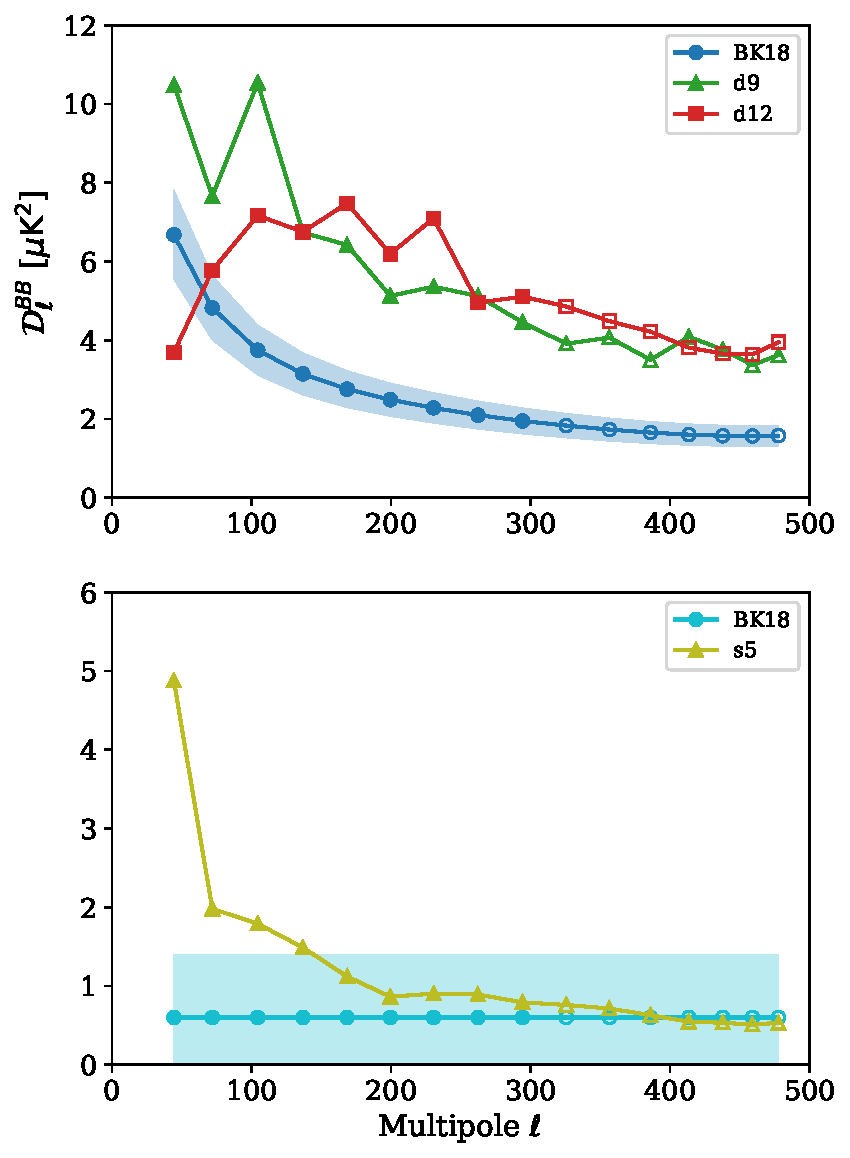
\includegraphics[width=0.48\textwidth]{figures/BKfield_power.pdf}
    \caption{Comparison between PySM $BB$ power spectra of the BK patch and the BK18 maximum likelihood models, with the top and bottom panels showing the dust and synchrotron results at 353~GHz and 23~GHz respectively. The first 9 band powers are denoted in solid marker as they are the BK science bins used for delivering constraints. The shaded area represents an uncertainty in foreground amplitudes ($\pm 0.75 \; \mu\rm{K_{CMB}}^2$ for dust and a 95\% upper limit $1.4 \; \mu\rm{K_{CMB}}^2$ synchrotron) extracted from BK18 MCMC constraints.}
    \label{fig:BKfield_power}
\end{figure}

Figure~\ref{fig:psym_BKmatrix} presents PySM dust model \texttt{d9} maps that are ``reobserved'' to emulate the impact of the BK timestream processing and map-making pipeline. In the first panel, the \texttt{d9} $Q$/$U$ maps at 353~GHz are masked to the BICEP3 observation region and convolved with the BICEP3 beam. The next panel shows the results after multiplying these smoothed maps with the BK18 BICEP3 observation matrix to capture the processing steps of data reduction \citep[e.g., filtering applied along RA scans,  beam deprojection in the linear map-making process][]{BICEP2Collaboration:2016}. Multiplying the input maps with this matrix produces output maps that appear as if they have been observed and analyzed through the BICEP3 pipeline. As an effect of filtering, these maps lose their large-scale structures and the amplitude of fluctuations is decreased by a factor of 10. In the third panel, the intermediate maps are multiplied by the corresponding purification matrix to remove $E$-$B$ mixing, resulting in pure $B$-mode dominated $Q$ and $U$ maps with clear ``cross-like'' and ``plus-like'' pattern respectively. To yield the final science maps, the inverse noise-variance apodization mask is applied as well.

Applying the same process to other PySM models at frequencies of interest (\texttt{s4}, \texttt{s5}, \texttt{s6}, \texttt{s7} at 20, 23, 30, 40~GHz and \texttt{d9}, \texttt{d10}, \texttt{d12} at 85, 150, 220, 270, 353~GHz), we acquire a set of BK pipeline propagated, pure $B$-mode model foreground maps compatible with BK measurements. We then proceed to calculate their $BB$ auto power spectra using the BK binning and present selected results in this section. 

In Figure~\ref{fig:BKfield_power}, we show the \texttt{d9} and \texttt{d12} $BB$ band power at 353~GHz and the \texttt{s5} band power at 23~GHz, the pivot frequencies adopted in the BK analyses. These PySM power spectra are compared with the BK18 maximum likelihood foreground model comprising a modified blackbody power spectrum ($T_d$ fixed at $19.6~\text{K}$) with parameter $A_{d,\ell=80} = 4.4 \; \mu\rm{K_{CMB}}^2$, $\beta_d = 1.5$ and $\alpha_d = -0.66$ for dust, and a square-law power spectrum with parameter $A_{s,\ell=80} = 0.6 \; \mu\rm{K_{CMB}}^2$, $\beta_s = -3.0$ and $\alpha_s = 0.00$ for synchrotron. These BK18 model lines are further suppressed by their band power window functions to account for the mode loss and mode coupling induced by the matrices. All band powers are eventually converted to full-sky $D_\ell$ by a division of the integral of the band power window function.

While models \texttt{d9} and \texttt{d10} generally display a spatial variation that can be described by a power law, we find that \texttt{d12} has a fall in power in low-$\ell$ regime as it has a fairly smooth map region at the upper left corner of the patch, different than the one being shown in Figure~\ref{fig:psym_BKmatrix}. Notably, all of them have excess $BB$ power compared to the measured amplitude in this patch of sky at 353~GHz. We thus further show the deviation ratios of these models down to 85~GHz in table~\ref{tab:BB_dustratio} to demonstrate how their amplitudes vary over frequency. It is found that \texttt{d9} and \texttt{d12} have a fairly stable factor of 2 deviation, but \texttt{d10} deviates less from the measurement as frequency decreases, pointing to a preference for a slightly smaller $\beta_d$. At larger scales of $\ell \lesssim 80$, these models are dominated by the underlying GNILC template, so the mismatch in amplitude between the BK maximum likelihood model and our templates is most likely due to residual noise in the GNILC template. Indeed, most of the constraining power on dust $BB$ power from~\cite{Ade:2021} is driven by BK measurements at 220~GHz, which are not used to inform our model.

%In Figure~\ref{fig:d1d9_bkpatch} we compare the BB power spectrum of the new \dnine{} model with the original PySM \done{} model, the GNILC input map, and the maximum likelihood dust model in this patch of sky determined from a combination of BK, Planck and WMAP data \citep{Ade:2021}. Model \done{} clearly has excess dust BB power compared to the measured amplitude in this patch of sky, which has been known for some time. This is somewhat ameliorated in model \dnine{}, primarily due to the steeper spectral tilt of the \dnine{} model leading to a factor of $\sim 10$ decrease in power relative to \done{} by multipoles of $\ell \gtrsim 300$. At larger scales of $\ell \lesssim 50$ both the \done{} and \dnine{} models are dominated by the underlying GNILC template, rather than the simulated small scale realizations, and so the mismatch in amplitude between the BK maximum likelihood model and our templates is most likely due to residual noise in the GNILC template. Indeed, most of the constraining power on dust BB power in Ref~\cite{Ade:2021} is driven by BK observations at 220\,GHz, which are not used to inform our model. 

The dust $BB$ amplitudes of the \texttt{d9}, \texttt{d10} and \texttt{d12} model disagree with existing observations in the BK patch of sky. However, it is beyond the scope of this work to provide full sky simulations that guarantee consistency with all sets of full sky and partial sky observations. Indeed, the use of power spectrum-based techniques requires a certain amount of global averaging of power spectrum parameters that are in fact known to vary across the sky \citep{planck2016-l04}. For example, while the dust amplitude can be modulated by the use of a large scale template, the spectral tilt $\alpha_{BB}$ has to be fixed to a single value for the full sky, which is not realistic.

%One may argue that the amplitude and spectral tilt of the \dnine{} model clearly disagree with existing observations in the BK patch of sky. While this is true, it is beyond the scope of this work to provide full sky simulations that guarantee consistency with all sets of full sky and partial sky observations. Indeed, the use of power spectrum-based techniques requires a certain amount of global averaging of power spectrum parameters that are in fact known to vary across the sky \cite{planck2016-l04}. For example, while the dust amplitude can be modulated by the use of a large scale template, the spectral tilt has to be fixed to a single value for the full sky, which is not realistic.

%\begin{figure}[ht]
%    \centering
%    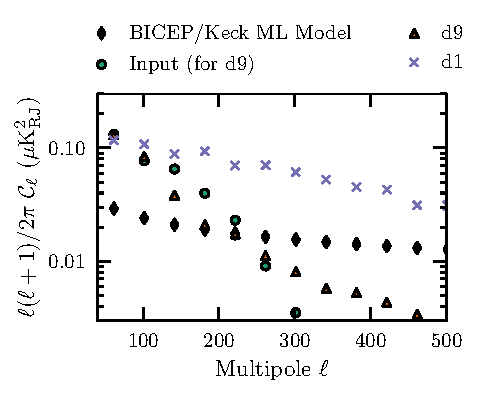
\includegraphics{paper_BK_patch.pdf}
%    \caption{This figure shows the BB power spectra of the \done{} (crosses), \dnine{} (triangles), and varres GNILC map (circles), compared to the maximum likelihood BK dust model (black diamonds) derived from a combination of WMAP and Planck with BICEP / Keck data up to the 2018 observing season. Note that in order to make a meaningful comparison between the bandpowers calculated from maps and the theory curve, we first convolve the theory spectrum with the mode-coupling matrix and then compute the decoupled bandpowers by applying the inverted binned coupling matrix.}
%    \label{fig:d1d9_bkpatch}
%\end{figure}

We present only the 23\,GHz PySM \texttt{s5} power spectrum in the lower panel of Figure~\ref{fig:BKfield_power} as other new models yield similar results. These models clearly exhibit a non-zero $\alpha_s$ and significantly larger power in $\ell \lesssim 100$ when the frequency is 23~GHz. However, this trend reverses at 40~GHz, where the synchrotron amplitude from the BK data becomes several times larger than that in \texttt{s5}, suggesting that the models have a more negative $\beta_s$ than the true sky in this region. While there is an inconsistency of synchrotron power in large scales between our models and the data, it is important not to overinterpret the discrepancies in $\alpha_s$ and $\beta_s$ since the latest BK results provide weak constraints on these two parameters, relying on reprocessed WMAP 23/33~GHz and NPIPE 30/40~GHz maps in the sky patch. Revisiting the discrepancies will be interesting when new synchrotron measurements are released from the BICEP Array telescope which comprises a dedicated 30/40~GHz receiver~\citep{Moncelsi:2020}.

\begin{table}
    \centering
    \begin{tabular}{lccccc}
    \toprule 
     & 85~GHz & 150~GHz & 220~GHz & 270~GHz & 353~GHz \\
    \midrule
    \texttt{d9}  & 2.17 & 2.12 & 2.08 & 2.06 & 2.03 \\
    \texttt{d10} & 0.96 & 1.30 & 1.59 & 1.77 & 2.03 \\
    \texttt{d12} & 2.76	& 2.27 & 2.08 & 2.02 & 1.96 \\
   \bottomrule
    \end{tabular}
    \caption{The deviation ratio of the reobserved PySM dust $BB$ spectrum to the BK18 maximum likelihood model at each delta frequency. These ratios are derived by fitting the BK18 model to the PySM band power at their science bins.}
    \label{tab:BB_dustratio}
\end{table}

% BH

%The new synchrotron models, s4, s5 and s7, have more power in the BICEP/Keck patch when compared to the old s1 synchrotron model. The latest BICEP/Keck results only has weak detection of synchrotron. We find that both the old and new PySM models are consistent with the BICEP/Keck upper limit on the synchrotron power. However, the BICEP/Keck maximum likelihood model for synchrotron has a better agreement with the new synchrotron models s4, s5 and s7 than with the old s1 synchrotron model. Thus, the new small scale generation in the synchrotron models s4, s5, and s7 increases the synchrotron power in the BICEP/Keck patch and is in better agreement with the constraints from the latest BICEP/Keck results.

\subsection{Decorrelation} \label{subsec:decorrelation}

One of the most challenging aspects of dust emission for CMB analyses is that its frequency dependence varies across the sky. If dust had the same SED everywhere, it would be sufficient to measure it at a frequency where it dominates the submillimeter emission and then subtract off all emission in lower frequency maps that is correlated with that template. The extent to which a map of dust emission at one frequency differs from a map of dust emission at a different frequency (aside from an overall normalization) is referred to as ``frequency decorrelation.'' Frequency decorrelation has been identified as a major uncertainty for ongoing and upcoming analyses \citep{Ade:2021}.

The level of decorrelation between two frequencies $\nu_1$ and $\nu_2$ can be quantified by the spectral correlation parameter $R_\ell$, defined as

\begin{equation} \label{eq:R_ell}
    \mathcal{R}^{XY}_\ell(\nu_1\times\nu_2) = \frac{\mathcal{D}_\ell^{XY}(\nu_1\times\nu_2)}{\sqrt{\mathcal{D}_\ell^{XY}(\nu_1\times\nu_1)\mathcal{D}_\ell^{XY}(\nu_2\times\nu_2)}}
    ~~~,
\end{equation}
where $X$ and $Y$ can be any of $T$, $E$, or $B$ \citep{planck2016-L}. Here we focus on $R_\ell^{BB}$.

The 353 and 217\,GHz Planck channels have the highest sensitivity to polarized dust emission and so furnish the current best constraints on the level of dust decorrelation. Analyzing 71\% of the sky over multipoles $50 \leq \ell \leq 160$, \citet{planck2016-l11A} found $R_\ell^{BB} > 0.991$ (97.5\% confidence) between these two frequencies.

\begin{figure}
    \centering
    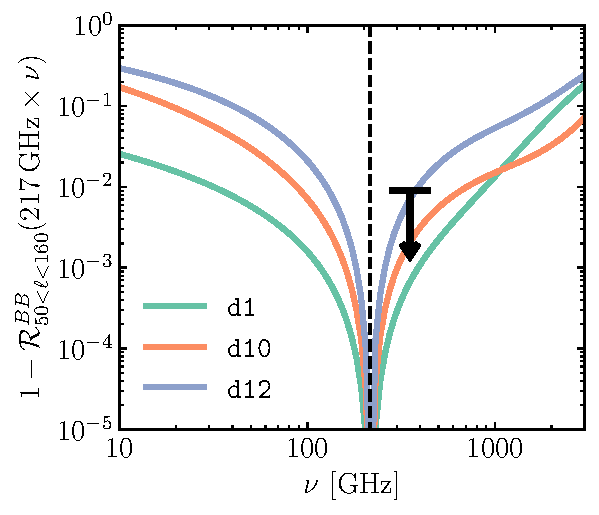
\includegraphics[width=\columnwidth]{figures/decorrelation_dust.pdf}
    \caption{The decorrelation parameter $1-R_\ell^{BB}$, where $R_\ell^{BB}$ is the correlation parameter defined in Equation~\eqref{eq:R_ell}, for the \texttt{d1}, \texttt{d10}, and \texttt{d12} dust models between a reference frequency of 217\,GHz and variable $\nu$. $R_\ell$ is evaluated between $50 \leq \ell \leq 160$ over the Planck 70\% sky mask. The 95\% upper limit on decorrelation derived by \citet{planck2016-l11A} over 71\% of the sky is indicated by the black arrow at 353\,GHz. The models span a large range in decorrelation level and each has a distinctive dependence on frequency.}
    \label{fig:decorrelation}
\end{figure}

In Figure~\ref{fig:decorrelation}, we compare the \texttt{d1}, \texttt{d10}, and \texttt{d12} models to this upper limit and analyze more generally how the level of decorrelation with respect to the 217\,GHz map changes with frequency. For each model, we compute $R_\ell^{BB}\left(217\times\nu\right)$ over the multipole range $50 \leq \ell \leq 160$ over the GAL70 mask as a function of $\nu$. We adopt a uniform weighting to average the spectra over the broad multipole bin since $\mathcal{D}_\ell^{BB}$ for dust scales roughly as $\ell^{-0.5}$ (see Table~\ref{tab:smallscale_par}). However, nearly identical results are obtained with uniform weighting in $C_\ell$ instead.

We find that all three models respect the upper limit set by \citet{planck2016-l11A}, with \texttt{d12} coming closest to saturating it ($R_\ell^{BB}(217\times353) = 0.9930$), then \texttt{d10} (0.9979), then \texttt{d1} (0.9993). The models thus span a range of viable levels of decorrelation. Because the spectral parameters ($T_d$ and $\beta_d$) of the \texttt{d9} model do not vary across the sky, that model has no decorrelation by construction (i.e., $R_\ell = 1$).

It is noteworthy that the frequency dependence of $R_\ell^{BB}(217\times\nu)$ is different for each model. For instance, the \texttt{d1} model has less decorrelation than \texttt{d10} at frequencies near 217\,GHz but more decorrelation at $\nu \gtrsim 1$\,THz. At frequencies much lower than the peak of the dust SED, the dust emission is in the Rayleigh-Jeans tail of the Planck function and is thus linearly proportional to $T_d$. In this limit, $T_d$ cannot contribute to frequency decorrelation as changes in $T_d$ do not affect the ratio of the emission in two bands. At low frequencies, then, decorrelation is sensitive only to variations in $\beta_d$. In contrast, dust emission near the peak is a non-linear function of $T_d$, rendering changes in the dust temperature much more important to decorrelation. The \texttt{d1} model is based on component separation with Commander that placed a Gaussian prior on $\beta_d$ with $\sigma_{\beta_d} = 0.1$ \citep{planck2014-a12}. Therefore, most of the observed variability of the dust SED is explained in this model via fluctuations in $T_d$. Further, the Commander data model did not account for CIB fluctuations, and so the resulting maps of dust parameters have enhanced small-scale fluctuations from CIB contamination. In contrast, the component separation based on GNILC that led to the $T_d$ and $\beta_d$ maps used in the \texttt{d10} model \citep{planck2016-XLVIII} permitted large variations in $\beta_d$ and largely removed CIB fluctuations. Indeed, the Commander-based parameter maps have less variance in $\beta_d$ and more variance in $T_d$ than the parameter maps from the GNILC-based analysis \citep[see][Table~1]{planck2016-XLVIII}. The result is that \texttt{d10} predicts much larger values of decorrelation than \texttt{d1} at low frequencies where $\beta_d$ is the dominant driver of decorrelation, but somewhat smaller values at high frequencies where $T_d$ is the dominant driver.

At present, it is unclear whether \texttt{d1}, \texttt{d9}, \texttt{d10}, or \texttt{d12} is a more accurate description of the spatial variability of $T_d$ and $\beta_d$ and thus of frequency decorrelation. Constraints on decorrelation at higher frequencies where the models diverge most sharply would enable more accurate predictions for the level of decorrelation expected at CMB frequencies. As component separation techniques continue to improve by incorporating information in both the pixel domain and the harmonic domain, and as new data sets are becoming available, it is also timely to revisit the component separation analysis with the aim of making improved $T_d$ and $\beta_d$ maps.

\subsection{Extragalactic contamination} \label{sec:CIBcontamination}

%[Stanford student Monica Hicks is working with Susan on cross-correlating our models with galaxy surveys a la Chiang \& Menard.] 

\begin{figure}[ht!]
    \centering
    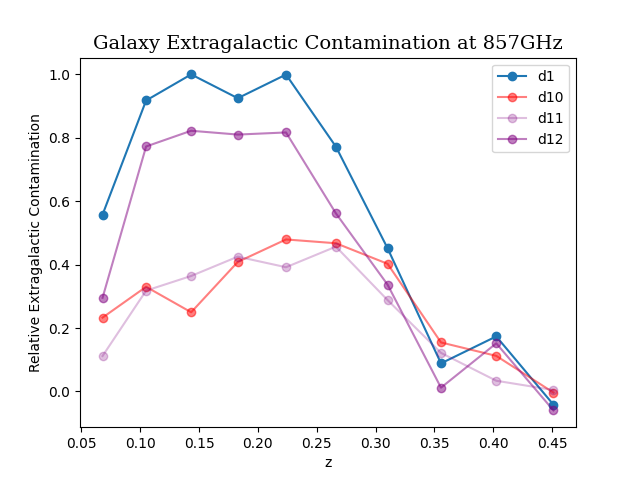
\includegraphics[width=\columnwidth]{figures/EGC_galaxy@857Part_0-1.png}
    \caption{Relative extragalactic contamination in three of the new dust templates (\texttt{d10, d11, d12}), compared to the \texttt{d1} model. Contamination is quantified as the excess 857 GHz emission within $11'$ of galaxies from the GLADE+ catalog, normalized to the maximum excess and plotted as a function of redshift (z). All three new dust templates contain less extragalactic contamination than older dust models because they are based on GNILC-processed Planck data. The improvement is most significant for \texttt{d10} and \texttt{d11}.  }
    \label{fig:extragal_contamination}
\end{figure}


%Our Galactic dust templates are based on measurements of the 
We quantify the extragalactic contamination present in our dust models using a tomographic redshift-clustering technique \citep{Schmidt:2015, Chiang:2019}. Our intensity-based Galactic dust templates inevitably contain emission from both Galactic dust and external galaxies. As described in Section \ref{sec:dustamplitude}, the new \texttt{d9} and \texttt{d10} dust templates are derived from GNILC-processed Planck data, while older PySM dust templates used \texttt{Commander} data products. We thus expect that the new Galactic dust models are significantly less affected by CIB contamination than previous models. Here we quantify this contamination by measuring the angular cross-correlation between our dust models and the clustering of galaxies as a function of redshift in spectroscopic survey data. A perfect Galactic dust template would be uncorrelated with such clustering; the signature of CIB contamination is excess template emission correlated with galaxy clustering. 

Following the procedure in \citet{Chiang:2019}, we compute the cross-correlation between local fluctuations in the Galactic emission maps and the galaxy density as a function of redshift, using galaxies from the GLADE+ catalog \citep{Dalya:2022}. We compute this cross-correlation for each of the \texttt{d1, d10, d11}, and \texttt{d12} dust emission templates at 857 GHz, at high Galactic latitudes ($\left|b\right| > 30\deg$). Figure \ref{fig:extragal_contamination} shows that while each of the new GNILC-based maps contain less extragalactic contamination than \texttt{d1}, the decreased contamination is more marked in \texttt{d10} and \texttt{d11} than in \texttt{d12}. This is likely due to [FILTERING CHOICES? TO DISCUSS WITH JACQUES]


\subsection{Non-Gaussianity} \label{sec:nongaussianity}

In this section, we aim at quantifying the level of non-Gaussianity in the small-scale dust emission generated through the polarization fraction tensor transformation using the simulations from PySM dust model \texttt{d10}.

To measure the non-Gaussianity in the maps we consider the Minkowski Functionals \citep[MFs,][]{Minkowski1903}, which are a common tool to quantify map-space  higher order statistical properties \citep{Martire:2023, Carones:2024}. Hadwiger’s theorem \citep{hadwigerVorlesungenUeberInhalt1957}
implies that, for any $n$-dimensional excursion set defined with a threshold value $\rho$, there exist $n+1$ MFs that geometrically and topologically describe the morphology of the set. In our case, for two-dimensional maps, we have three kinds of MFs, $\mathcal{V}_0$, $\mathcal{V}_1$ and $\mathcal{V}_2$ which correspond to the area, the perimeter and the connectivity of the excursion set, respectively.

We use these MFs to compare the small-scale structure in \texttt{d10} to those of two other sets of maps: (i) maps where small-scale structures are fully Gaussian and isotropic and (ii) maps where small-scale structures are Gaussian but modulated across the sky. The reason why we need the second set of maps is the following: as described Section \ref{subsec:methodology}, the small scale structures in \texttt{d10} model are generated as Gaussian field in $i$, $q$ and $u$ and multiplied with $m_i$ and $m_p$ modulation maps, before adding them to the large scale maps and transformed back into $I$, $Q$ and $U$. This procedure leads to an effective modulation of small scale structures on $I/Q/U$ maps. We want to understand what is the impact of this effective modulation on MFs, and therefore construct a set of maps which only takes into account this modulation applied to a Gaussian field directly on Stokes parameter maps, without any transformation into polarization fraction tensor analogues. This allows to disentangle the non-Gaussianity generated through modulation from the potential non-Gaussianity due to the polarization fraction tensor transformation.   
The first set of map, with Gaussian isotropic field is built as follows:
\begin{enumerate}

\item We first fit power laws to the $TT$, $EE$, $BB$ power spectra in the multipole range $[800, 2000]$ calculated from the \texttt{d10} maps on the \texttt{GAL097} mask. 

\item To retain only the small scales, we apply a high-pass filter to the fitted power law power spectra with $\ell_{cut} = 200$ for intensity and polarization maps, and then generate full sky small scales realizations of these filtered power law spectra (with $\ell_{max}=4096$) with the \texttt{synfast} routine provided by HEALPix. 

\item The generated Gaussian isotropic small scales are added to
the large-scale dust template to form the first final set of maps.

\end{enumerate}

For the second set, we need to mimic the effective modulation of \texttt{d10} maps in $IQU$ quantities. We use the following procedure:
\begin{enumerate}
\item We generated modulation maps in the same way as done in $iqu$ space (Eq. \ref{eq:mod_maps}), except that here we implemented them directly in $IQU$, therefore obtaining $m_I$ and $m_P$ for temperature and polarization.
\item We multiplied these modulation maps with maps of Gaussian isotropic small scales (generated as for the first set of Gaussian isotropic maps, as described in point 1 and 2 above) and coadd them with the large-scale dust template.
\item We compare the power spectra of these maps with those of \texttt{d10} on four different sky masks: \texttt{GAL40, 60, 80, 97}.

\item{We fine-tuned the $m_I$ and $m_P$ modulation maps, through multiplication factors in the sky regions defined by the four masks, in order to ensure that the power spectra compute on the different masks are as close as possible to the ones of \texttt{d10}. For each mask we only consider the part not overlapping with other masks, such as the yellow region in Fig.\ref{fig:sync_masks} showing the additional coverage of \texttt{GAL60} compared with \texttt{GAL40}}
\end{enumerate}


Now we have three sets of maps with different small scales co-added: model \texttt{d10}, a map with purely Gaussian small-scale structure, and a map with modulated Gaussian small-scale structure. %and the last from modulated Gaussian realization in the $IQU$ domain.
We apply a high-pass filter to retain only the small scales of these maps, which we will refer to as \texttt{poltens-ss}, \texttt{Gaussian-ss}, and \texttt{Gaussian-mod-ss}, respectively. We calculate the MFs both on the sphere and in several selected regions of the sky projected into a Cartesian projection. 

%Below we show the MFs calculated for these three sets of small scales on the sphere and also for a selected flat patch.

\subsubsection{Minkowski Functionals on the sphere}

Following the algorithm in \cite{Grewal:2022}, we calculate the MFs for the three $Q$ maps on the sphere, i.e., in HEALPix format, with a \texttt{GAL080} mask\footnote{\url{http://pla.esac.esa.int/pla/aio/product-action?MAP.MAP_ID=HFI_Mask_GalPlane-apo2_2048_R2.00.fits}}, which masks out the Galactic plane. We first normalize the maps by dividing each map by its standard deviation and retain only pixels with values $[-3, 3]$ over which to calculate the MFs. Results are shown in Figure~\ref{fig:MF:sphere}. The MFs of the corresponding $U$ maps look very similar to $Q$ maps and are not shown here.

Figure~\ref{fig:MF:sphere} shows that when averaging over a large sky area, the MFs of \texttt{Gaussian-mod-ss} and \texttt{poltens-ss} are almost identical, while the MFs of \texttt{Gaussian-ss} differ substantially. The difference in MFs between \texttt{poltens-ss} and \texttt{Gaussian-ss} implies the existence of non-Gaussianity in \texttt{poltens-ss}, but the similarity between \texttt{poltens-ss} and \texttt{Gaussian-mod-ss} demonstrates that the non-Gaussianity in \texttt{poltens-ss} comes from the anisotropy in the maps, which originates from the modulation, rather than from the polarization fraction tensor transformation.

\begin{figure*}
    \centering
    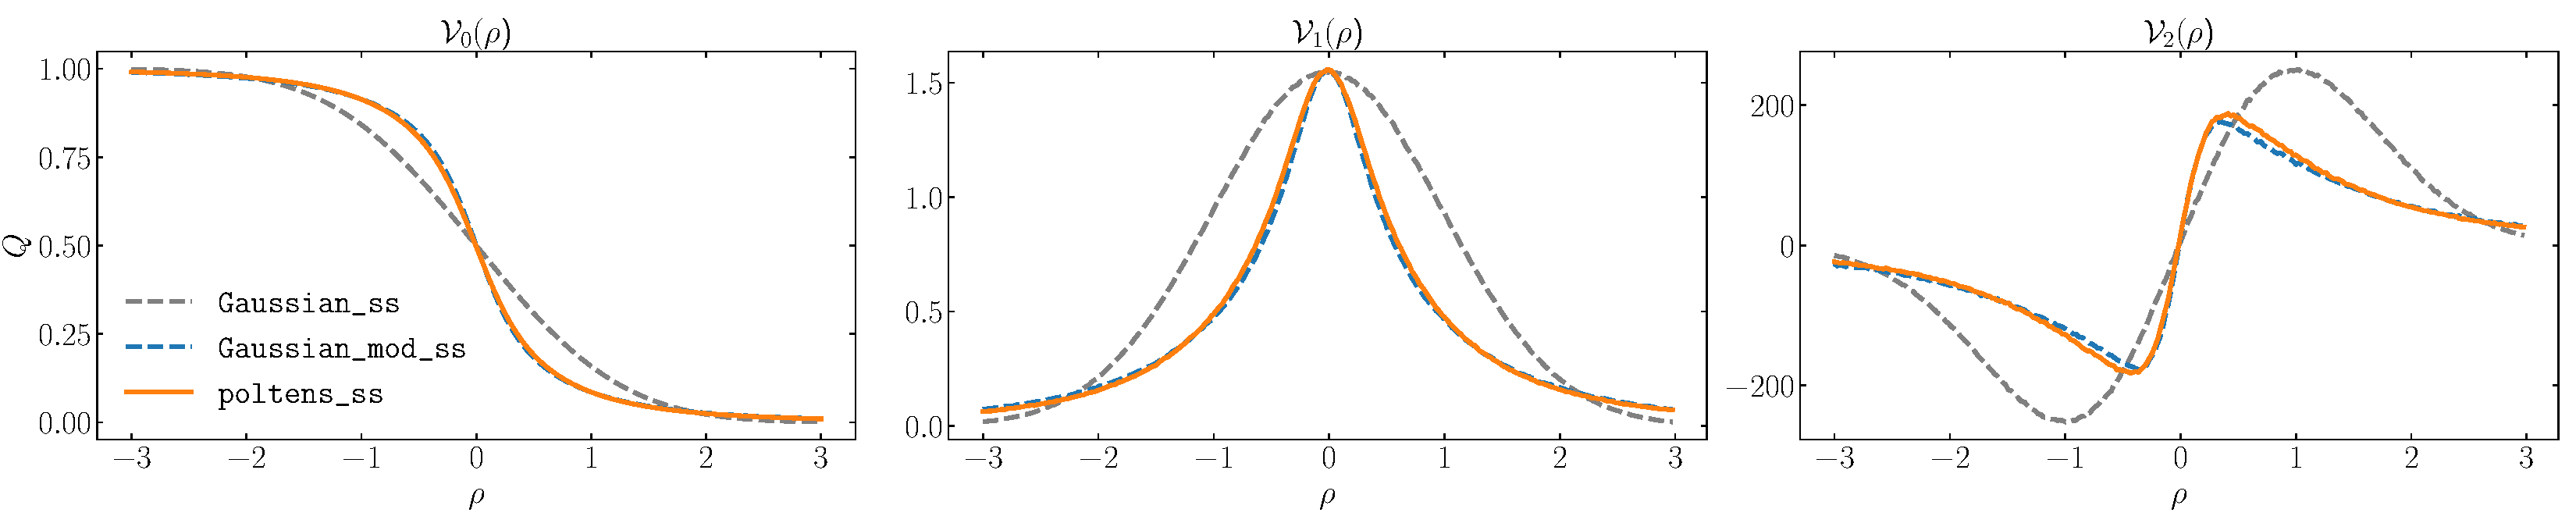
\includegraphics[width=180mm]{figures/MFs_80p_sky_Q.pdf}
    \caption{MFs for the small scales of three sets of maps on the sphere with \texttt{GAL080} mask. The large scales are filtered out by excluding multipoles $\ell < 200$ in the maps, and we choose $\ell_\text{max} = 2048$ when obtaining the small scales. We show the MFs as a function of threshold $\rho$, for \texttt{Gaussian-mod-ss} in blue, \texttt{poltens-ss} in orange and \texttt{Gaussian-ss} in dashed gray.}
    \label{fig:MF:sphere}
\end{figure*}

\begin{figure*}
    \centering
    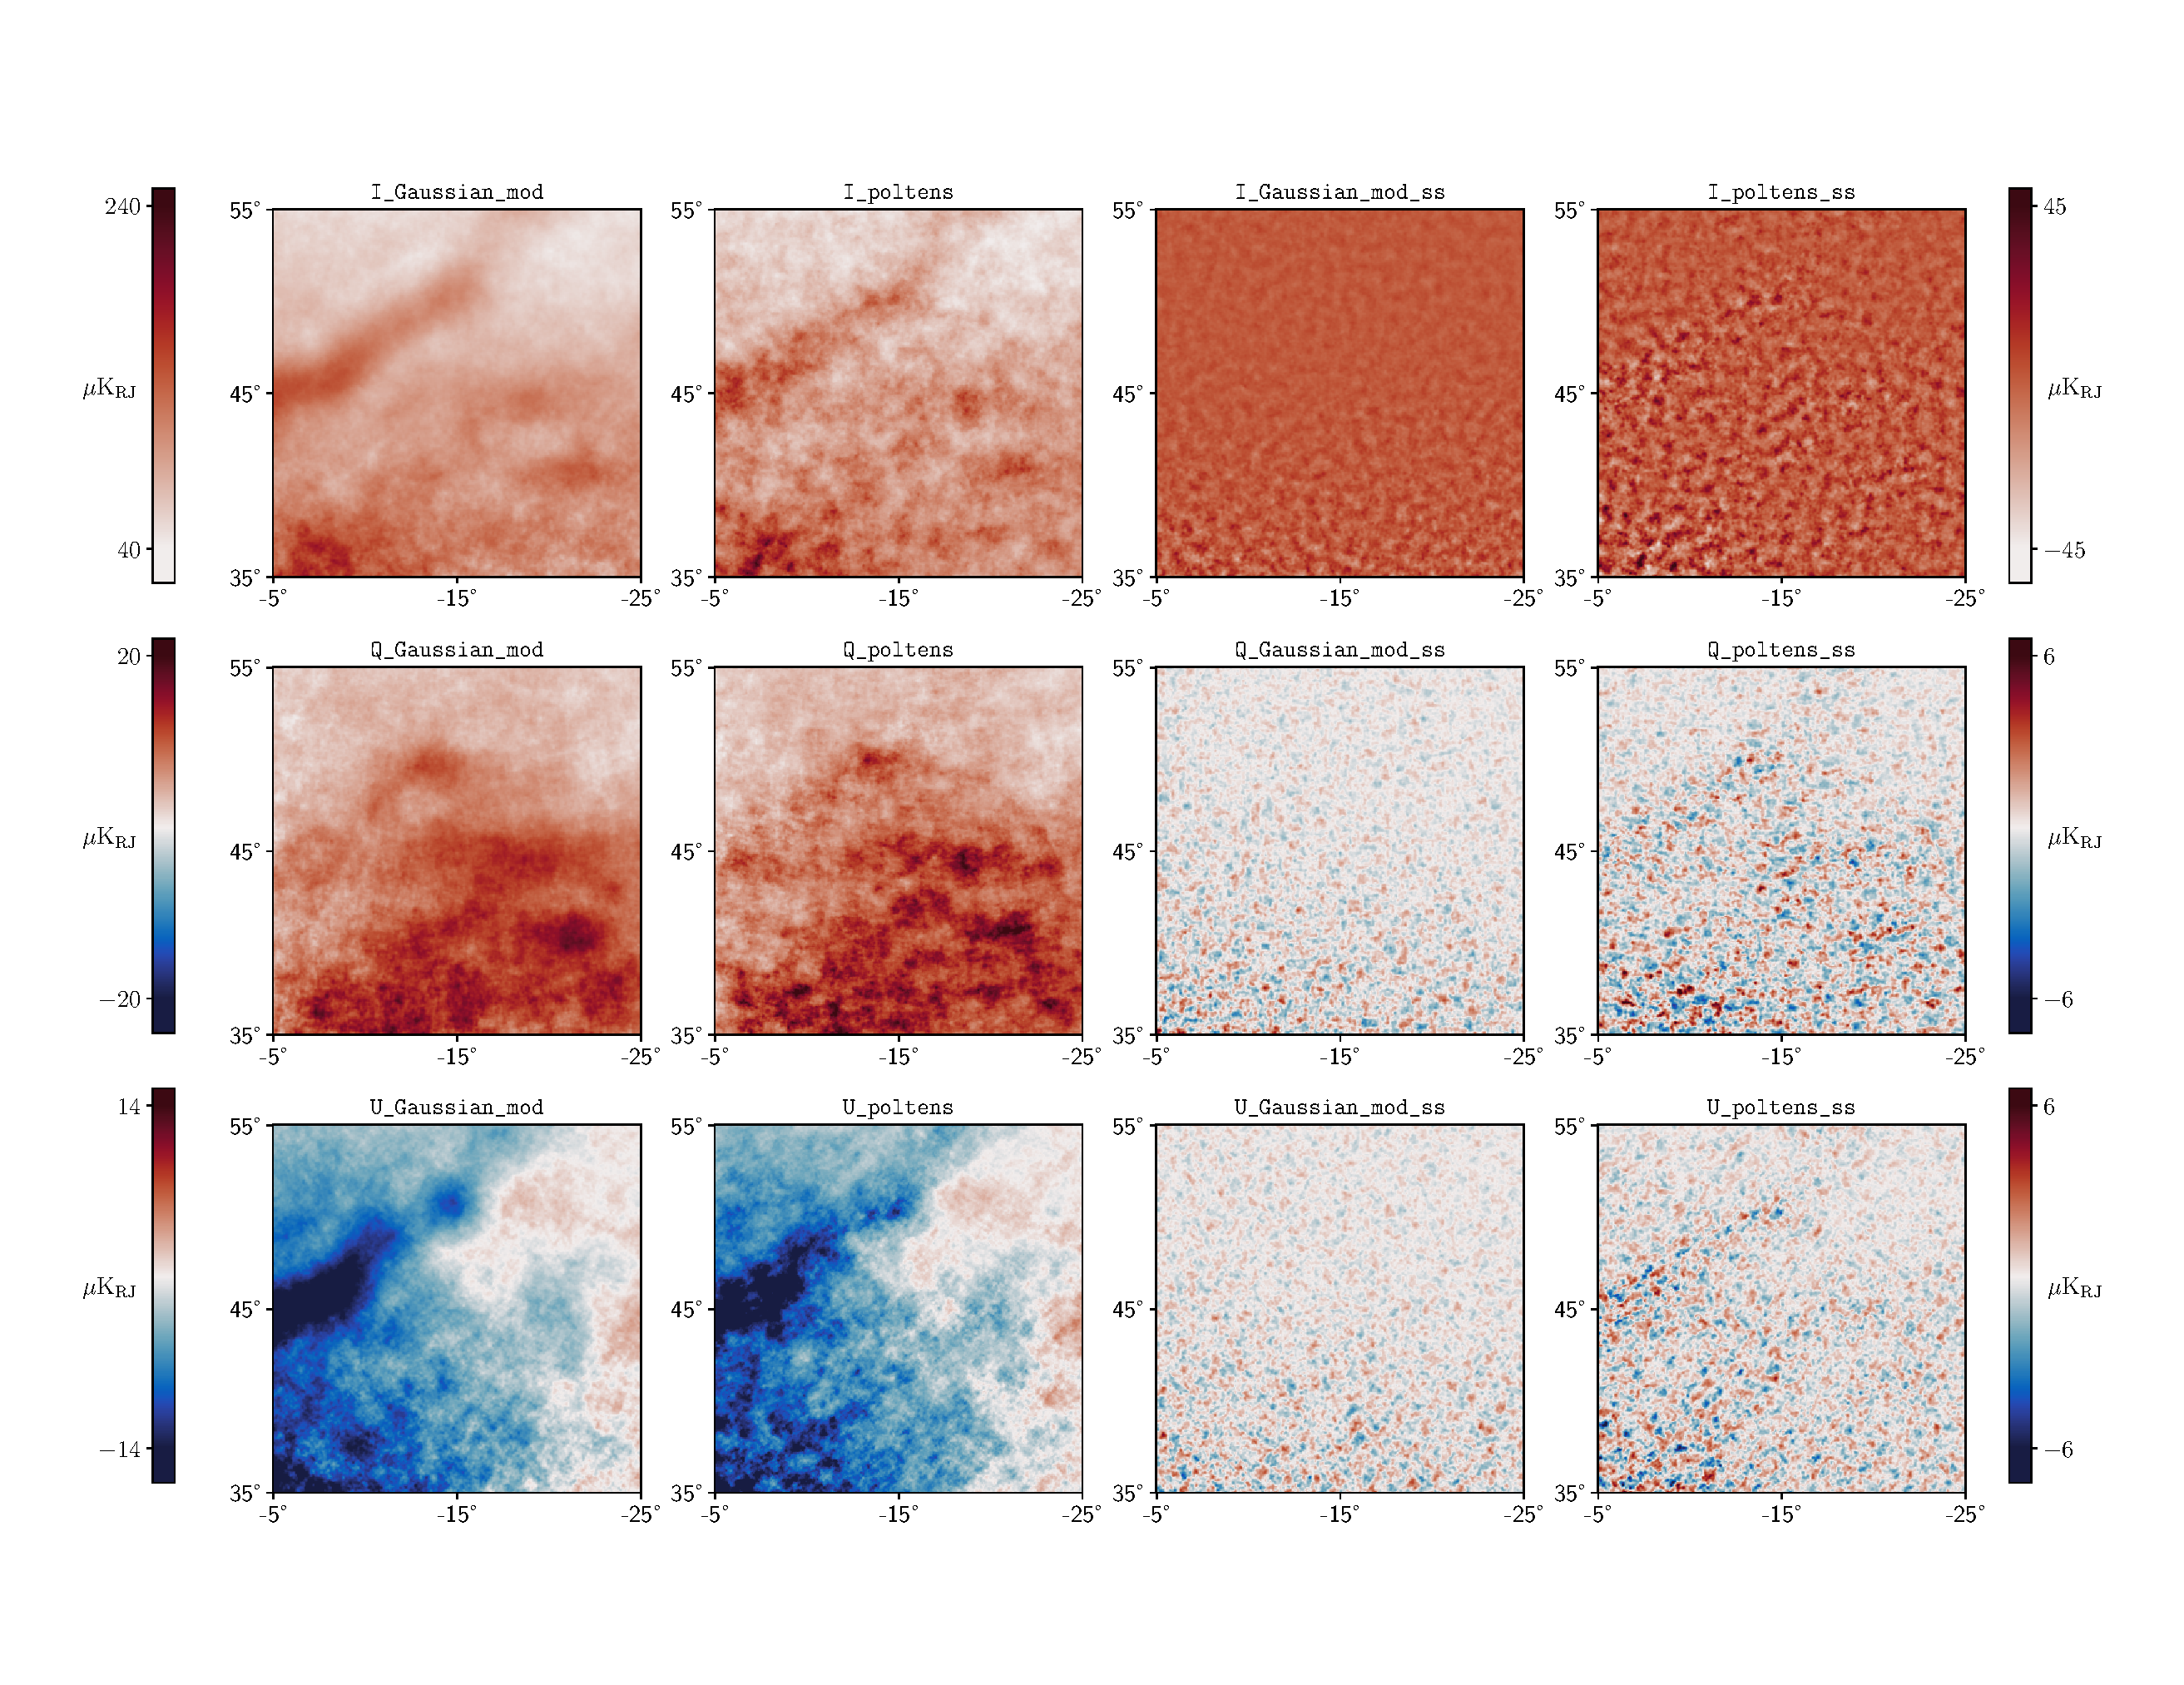
\includegraphics[width=180mm]{figures/maps_patch_345_45.pdf}
    \caption{We show the zoom-in plots in the selected patch at the center $(l, b) = (-15^{\circ}$, $45^{\circ})$, which are, from left to right, the final map with \texttt{Gaussian-mod-ss}, final map with \texttt{poltens-ss} (i.e., $\texttt{d11}$ map), \texttt{Gaussian-mod-ss} only map and \texttt{poltens-ss} only map. From top to bottom is for I, Q and U respectively. The colorbar on the left indicates the pixel values in the left-most two columns in the units of $\mu K_{RJ}$ and the colorbar on the right is for the last two columns. }
    \label{fig:maps:patch2}
\end{figure*}

\begin{figure*}
    \centering
    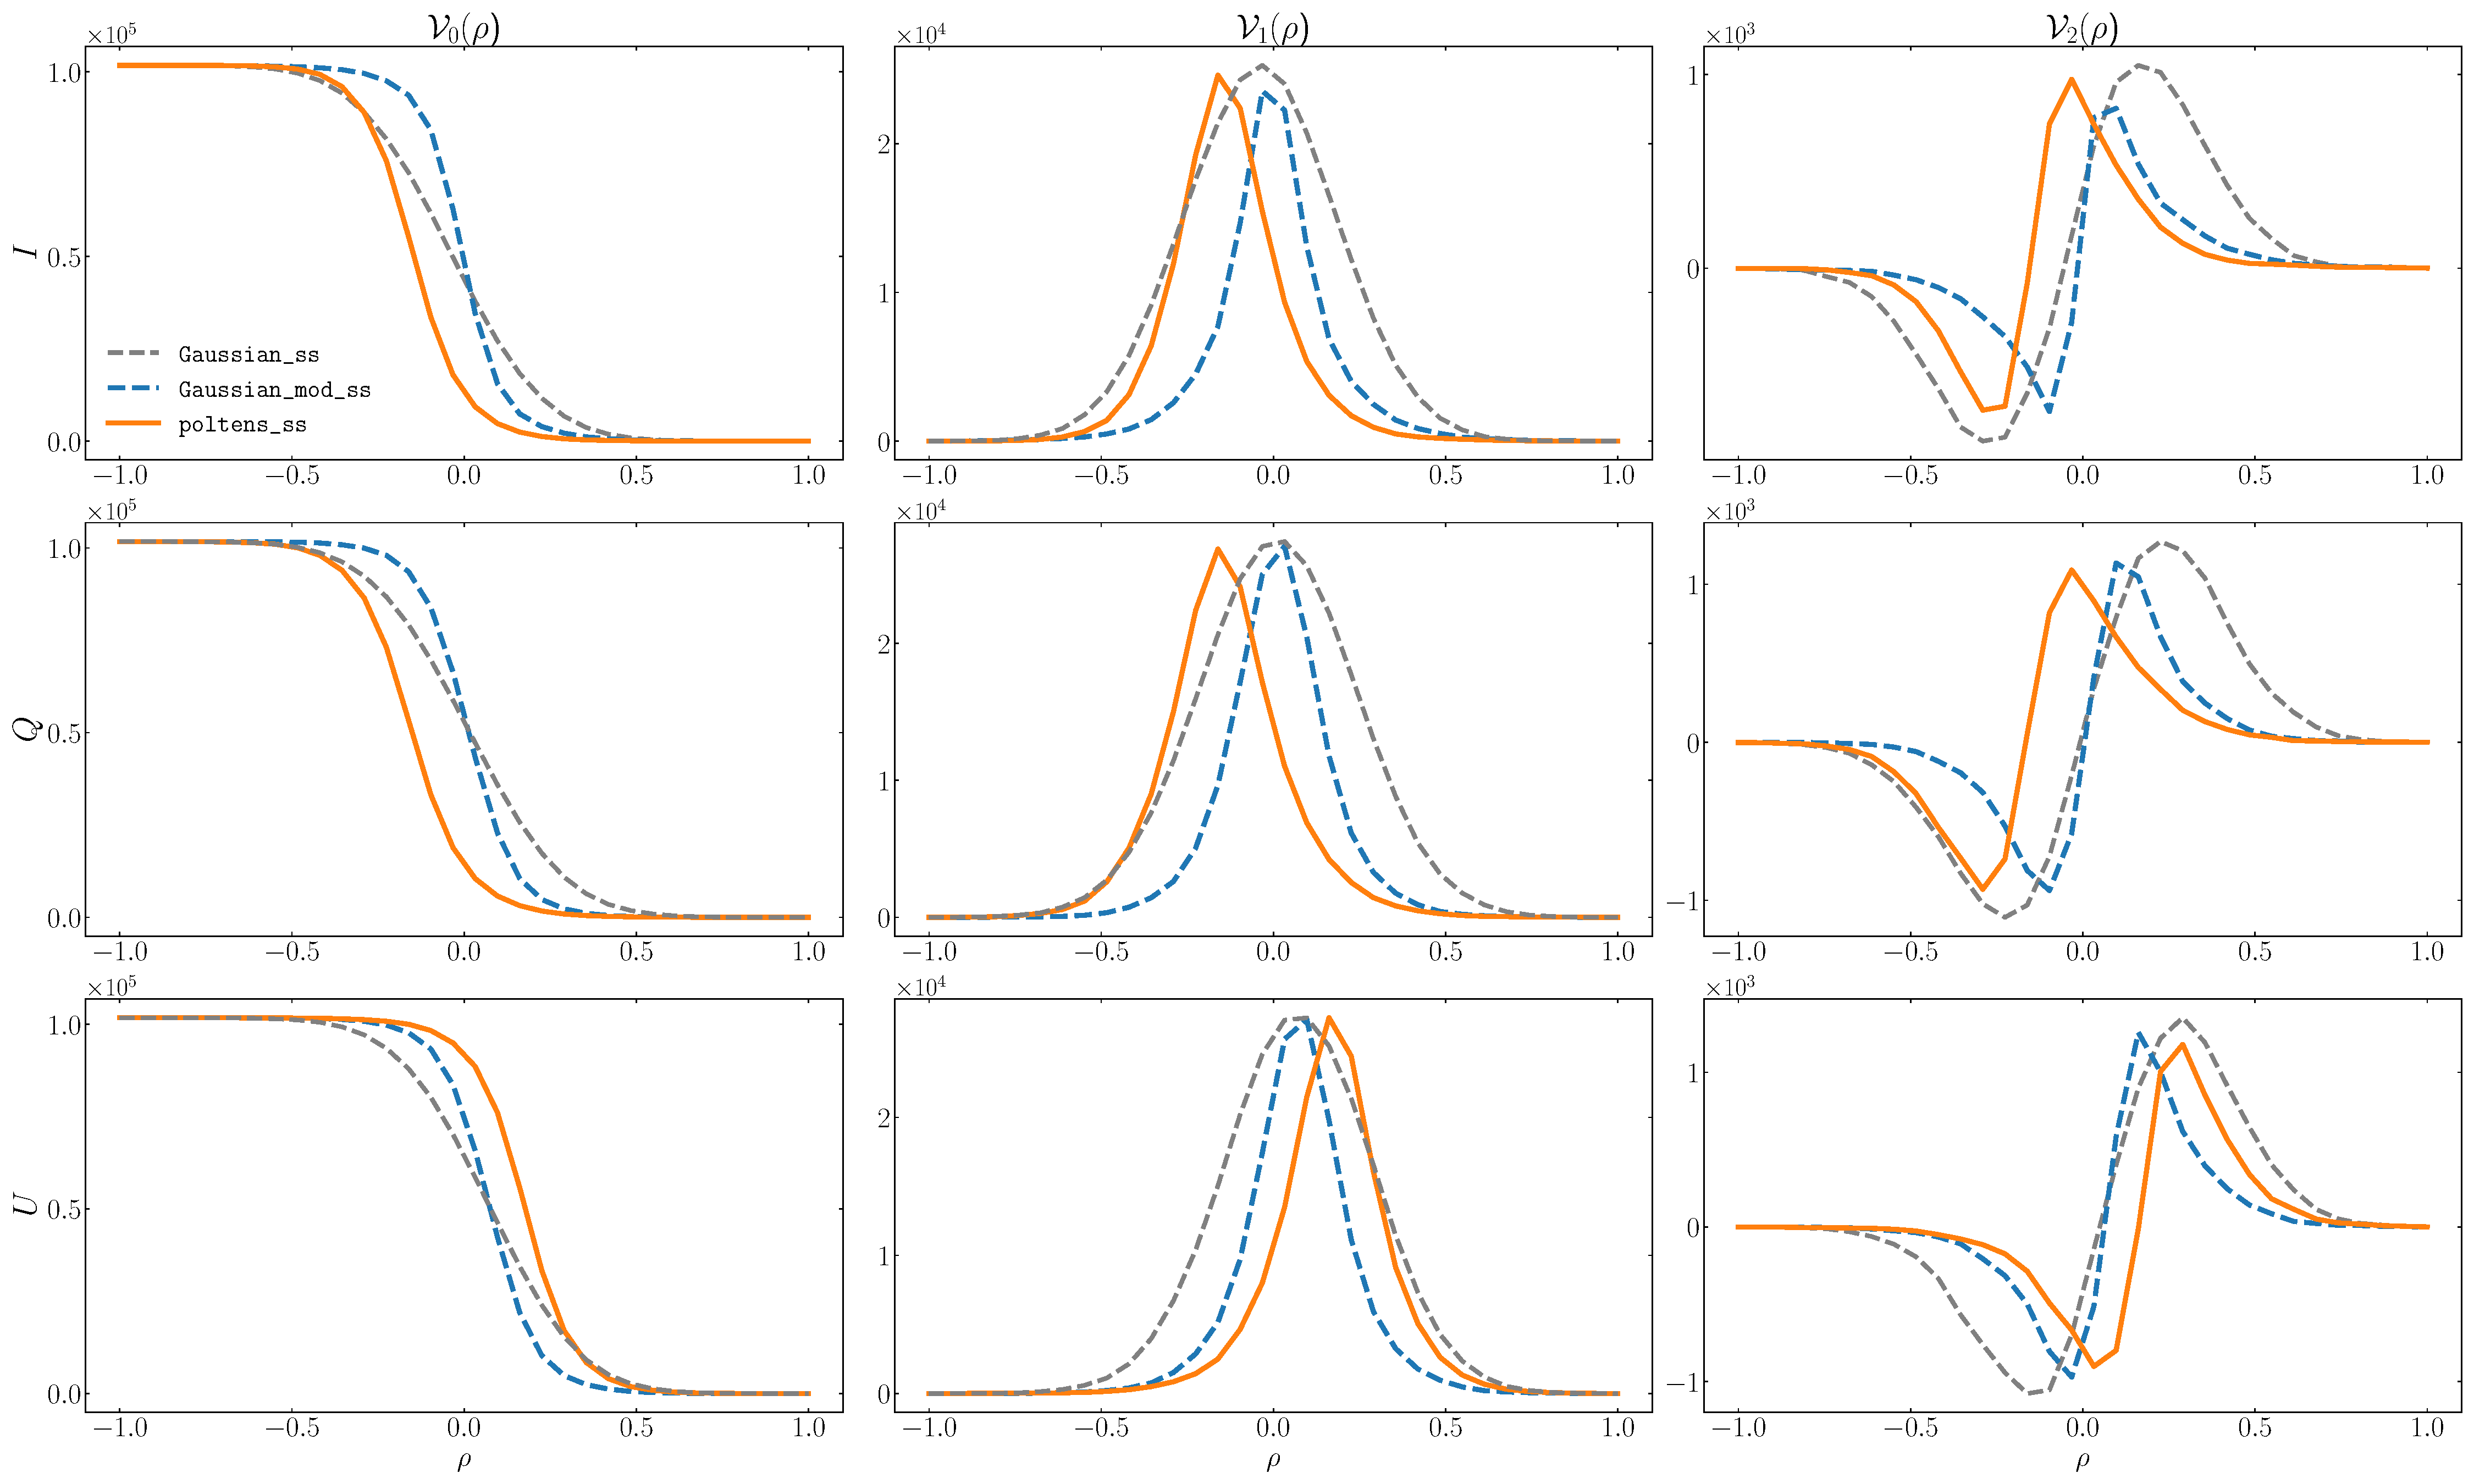
\includegraphics[width=180mm]{figures/MFs_345_45_with_G_rescaled.pdf}
    \caption{Minkowski Functionals as a function of the threshold $\rho$ for the one realization of I, Q and U small scales in the patch with center of $(l, b) = (-15^{\circ}$, $45^{\circ})$ in Galactic coordinates. Each row shows three kinds of Minkowski Functionals. The blue dotted one is for \texttt{Gaussian-mod-ss} while the orange solid one is from \texttt{poltens-ss}. We also show the \texttt{Gaussian-ss} in dashed gray line as a comparison.}
    \label{fig:MF:patch2}
\end{figure*}

\subsubsection{Minkowski Functionals on small regions}
We consider a region centered at $(l, b) = (-15^{\circ}$, $45^{\circ})$ with dimension of $20^{\circ}\times20^{\circ}$ to determine whether significant differences in the MFs between \texttt{Gaussian-mod-ss} and \texttt{poltens-ss} sets of maps exist in small regions of sky. Those maps are shown in Figure~\ref{fig:maps:patch2}. We can see by eye that \texttt{poltens-ss} contains structure that is not present in the \texttt{Gaussian-mod-ss} maps. We calculate the MFs of these small-scale maps, following \cite{Mantz:2008} for the calculation of MFs for a square patch. Before the calculation, we also rescale all the small scales linearly to be in the range [-1, 1], using the $minmax$ scheme.

Figure~\ref{fig:MF:patch2} shows the MFs of the \texttt{Gaussian-mod-ss} and \texttt{poltens-ss} maps presented in Figure~\ref{fig:maps:patch2}. In contrast with the large-area results presented in Figure~\ref{fig:MF:sphere}, in this case we do measure a departure of the \texttt{poltens-ss} MFs from the \texttt{Gaussian-mod-ss} ones. %This points towards the fact that the polarization fraction tensor transformation may indeed have induced some level of non-Gaussianity, distinct from pure modulation effects, that are detectable on small sky regions. 
This means that the polarization fraction tensor transformation introduced non-Gaussian small-scale structure, distinct from pure modulation effects, that is detectable on small sky regions. 
We conclude that the level of induced non-Gaussianity differs from one region to the other and does not significantly impact the statistical properties when averaged over large sky fractions.

% BH: The commented text below has been moved, but retained here for reference + original comments
% \subsection{Synchrotron validation} \label{sec:sync_validation}
% \textbf{Shamik:} \giuse{\sout{In this section we detail the validation of the new synchrotron models by comparing them with BeyondPlanck synchrotron map for temperature, and LFI 30\,GHz observations for polarization.}}  We compare the model with data at both  map and power spectrum  levels. For validating the PySM synchrotron temperature models, we use the synchrotron map from the BeyondPlanck re-analysis of Planck LFI data \citep{Anderson2023}. BeyondPlanck released a synchrotron map\footnote{https://beyondplanck.science/products/files\_v1} at a reference frequency of 30\,GHz and at $2^\circ$ angular resolution. We produce single frequency temperature maps for the different synchrotron models at 30\,GHz and smoothed with a Gaussian beam with FWHM = $2^\circ$.

% \giuse{In case of the synchrotron polarization, we  compare the models with band integrated observations. So, we compute bandpass integrated maps  with PySM~3 routines and for  the different synchrotron models. For the sake of fair comparison with \emph{Planck} data, we adopt the average LFI 30\,GHz RIMO transmission \citep{planck2014-a03}.} The bandpass integrated maps are further smoothed with Gaussian beams of 33.1 arcmin beams to produce model maps at native resolutions of the LFI 30 GHz data. Finally, the observed power spectra are computed by taking the cross-spectrum between independent detector splits, e.g. A and B, of the NPIPE \footnote{Publicly available through NERSC at \\ /global/cfs/cdirs/cmb/data/planck2020} (PR4) 30\,GHz maps \citep{planck2020-LVII}. 

% %\subsubsection{Galactic masks}
% \giuse{We estimated the synchrotron power spectra considering three choices of masks:  full sky  (100\%), 70\% and 50\% sky fractions. To produce the masks for the latter cases, we use the LFI 30\,GHz map of polarized intensity, smoothed with a Gaussian beam of $2^\circ$ FWHM, and masked all the pixels larger than  17 and 10 $\mu{\rm K}_{\rm CMB}$, and they are shown in Figure \ref{fig:sync_masks}.  Masks are apodized  with a $2^\circ$ cosine apodization.}
% \begin{figure}
%     \centering
%     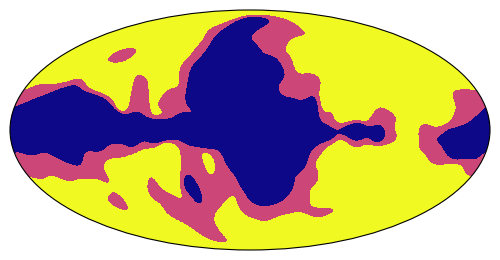
\includegraphics[width=0.46\textwidth]{figures/sync_galactic_mask.png}
%     \caption{Figure showing the two different Galactic masks used for the synchrotron validation. The yellow region is included by the 50\% sky mask, while the 70\% mask additionally includes the pink region.}
%     \label{fig:sync_masks}
% \end{figure}

% We use HEALPix \footnote{https://healpix.sourceforge.io} \texttt{anafast} function \citep{2005ApJ...622..759G, 2019JOSS....4.1298Z}  to compute the power spectra for the model and observation maps. For the polarization analysis, both the model and the LFI maps are additionally masked with the apodized LFI DR2 polarized point source mask. 
% For this validation test, we
% do not use a pseudo-$C_\ell$ estimator as the synchrotron signal is not statistically isotropic, and we correct for the partial sky by naively dividing by an $f_{\rm sky}$ factor.

% \begin{figure}
%     \centering
%     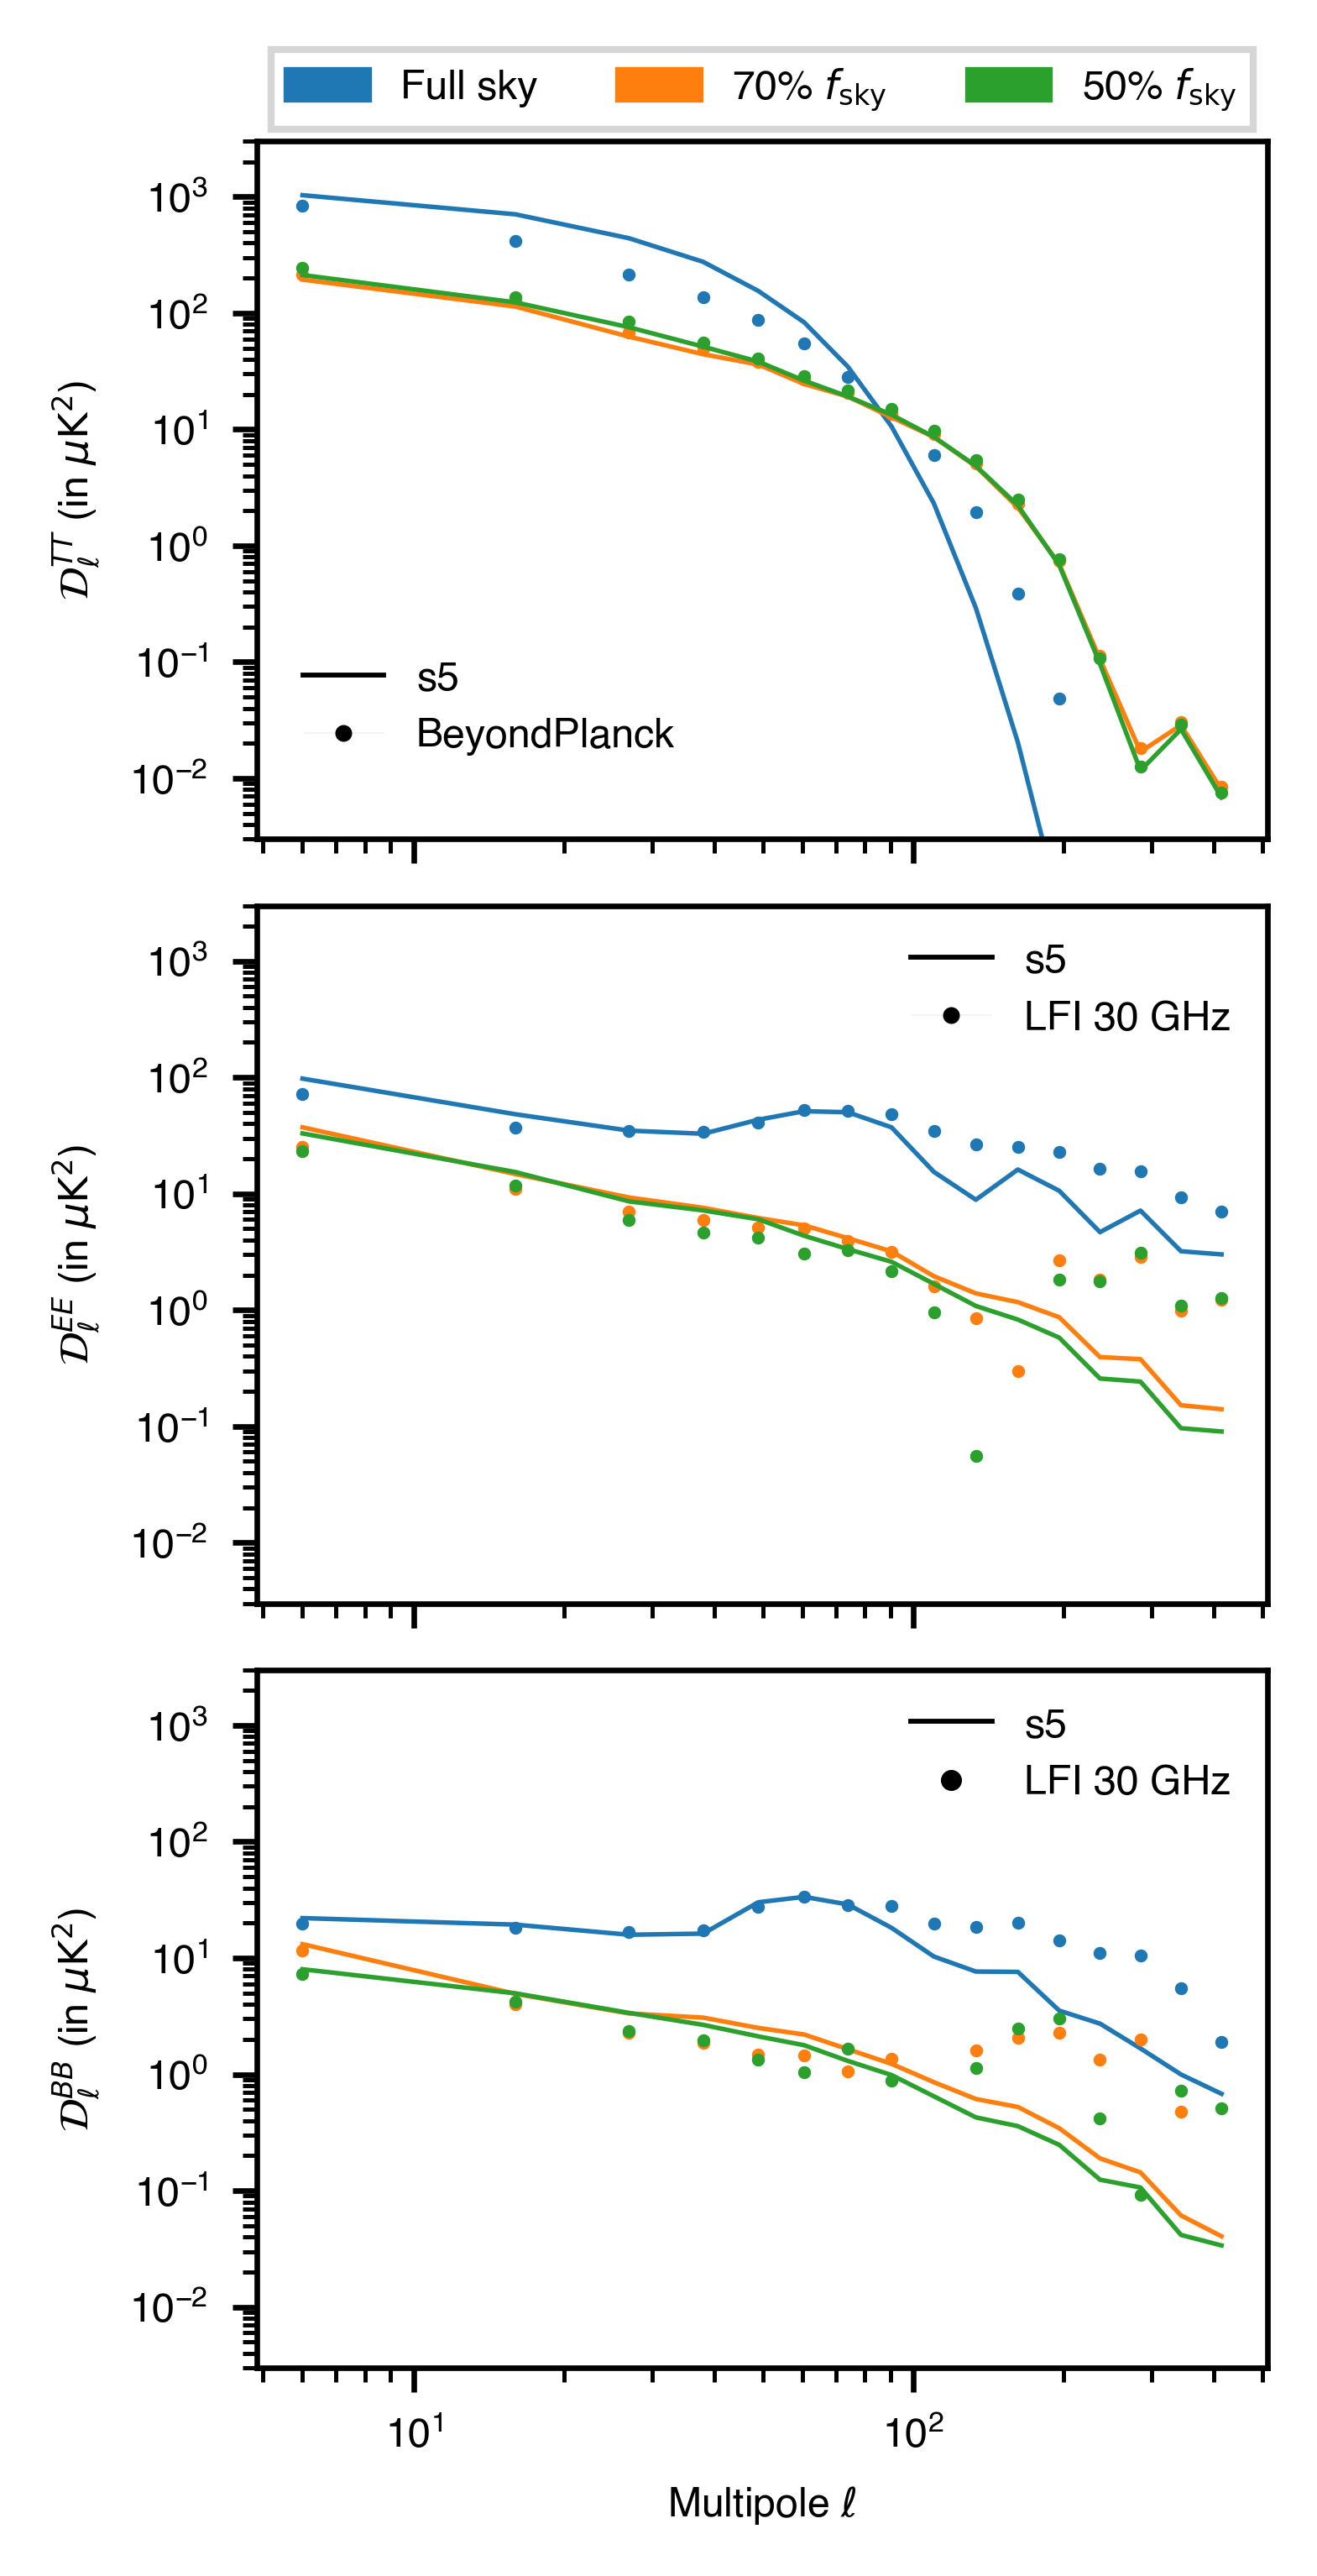
\includegraphics[width=0.48\textwidth]{figures/Dlcomp_PySM3-4b7_s5_vs_BPnLFI30_BPI.png}
%     \caption{Figure showing comparison of power spectra of the PySM s5 model with observation on different sky fractions. The spectra obtained for models s4, s6 and s7 are similar so we don't show them here. The $TT$ power spectrum comparison is done with synchrotron maps from BeyondPlanck release 1 \citep{Anderson2023}. The $EE$ and $BB$ power spectra is compared with NPIPE LFI 30\,GHz map \citep{planck2020-LVII}. The LFI 30\,GHz spectra are computed as a cross spectra between the NPIPE splits A and B.}
%     \label{fig:Dl_sync_galmask}
% \end{figure}

% The $TT$, $EE$ and $BB$ power spectra comparisons, for model s5, are shown in Figure~\ref{fig:Dl_sync_galmask}. The comparison for models s4, s6 and s7 have nearly identical results. The $TT$ power spectra for masked skies show excellent agreement with the BeyondPlanck synchrotron temperature power spectra. However, there is poor agreement for the full sky power spectra. On the full sky most of the spectra is dominated by what happens in the Galactic plane, which for observational data is contaminated by free-free and AME. Even with the BeyondPlanck component separation, the synchrotron power in the brightest sky regions is likely to have some residual contamination and associated uncertainty. The new PySM synchrotron models are difficult to assess in the regions of brightest galactic synchrotron emission and we caution users against using the synchrotron models in the brightest parts of the galaxy. However, going away from the galactic plane, we find excellent agreement with observations at power spectrum level.
% % So, it is reasonable to argue that for synchrotron temperature there is excellent agreement for all but the brightest parts of the sky, where the comparison is harder to make at 30\,GHz. 
% For polarization we find reasonable agreement at $\ell \lesssim 100$. For $\ell > 100$ the PySM synchrotron models typically have less power than the data. However, an important caveat is that despite the point source masking, there is some residual radio point source contribution to this power in the LFI maps.

% \begin{figure}
%     \centering
%     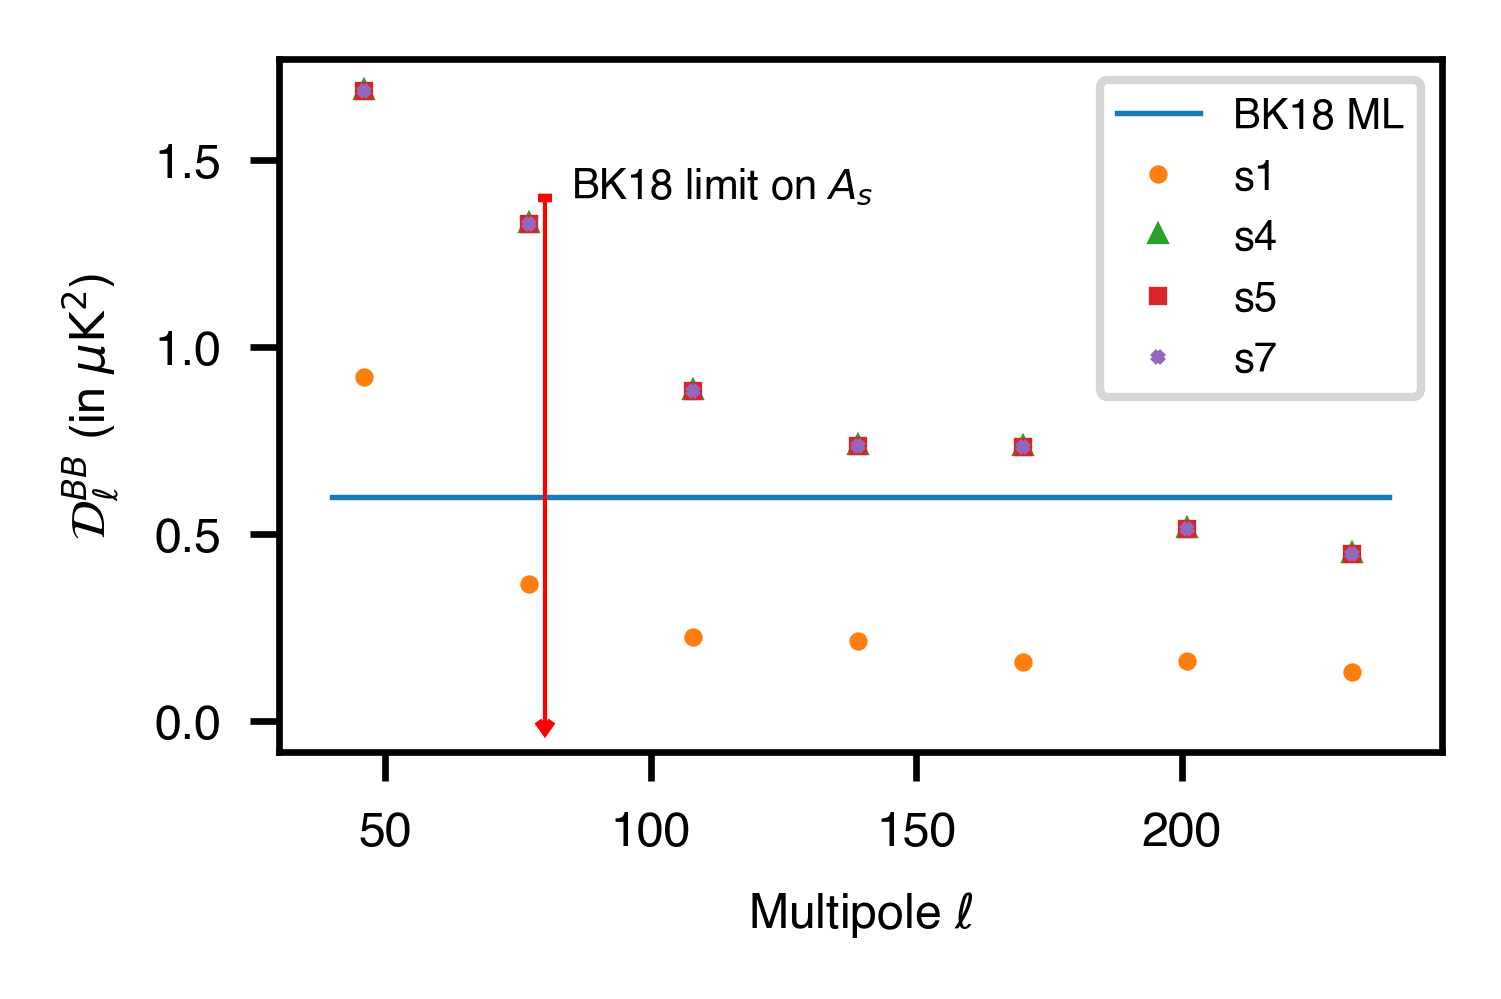
\includegraphics[width=0.49\textwidth]{figures/Dlcomp_PySM3-4b8_BKpatch.png}
%     \caption{Comparison of power spectra in the BICEP/Keck patch for the new PySM synchrotron models s4, s5 and s7 with old synchrotron model s1 and the limits on the synchrotron power obtained in BICEP/Keck 2018 \citep{Ade:2021} at the reference frequency of 23\,GHz. The blue line is the BICEP/Keck 2018 maximum likelihood model for synchrotron with $A_s=0.6 \mu {\rm K}^2$, $\alpha_s=0$. The red arrow indicates the BICEP/Keck 95\% confidence upper limit on $A_s<1.4 \mu {\rm K}^2$ after marginalizing over $-1<\alpha_s<0$ at $\ell=80$. The PySM synchrotron models s4, s5 and s7 have identical power spectra at 23\,GHz.}
%     \label{fig:Dl_sync_BK}
% \end{figure}

% \subsubsection{BICEP / Keck patch}
% The cleanest patch of sky in the southern hemisphere is particularly important for ongoing and future CMB experiments that target measurement of the primordial CMB B-modes. We focus on the small clean patch of sky that is targeted for the BICEP/Keck experiment for their constraints on the tensor-to-scalar ratio. This overlaps with the tentative sky patch that will be targeted by the CMB-S4 experiment for their primordial B-mode search \citep{CMB-S4:2020}. In their 2021 analysis the BICEP/Keck team placed a upper limit of $A_s<1.4 \mu{\rm K}^2$ at a pivot frequency of 23\,GHz with $\beta_s=-3.1$ after marginalizing over the range $-1<\alpha_s<0$ \citep{Ade:2021}. The BICEP/Keck maximum likelihood model for the synchrotron spectrum is parameterized by $A_s=0.6 \mu{\rm K}^2$, $\beta_s=-3.0$ and $\alpha_s=0$. In Figure~\ref{fig:Dl_sync_BK}, we compare these two sets of constraints from the BICEP/Keck 2018 results with the new PySM synchrotron models s4, s5 and s7. We also plot the old PySM s1 synchrotron model to show how the synchrotron model has changed in this patch of interest.

% The new synchrotron models, s4, s5 and s7, have more power in the BICEP/Keck patch when compared to the old s1 synchrotron model. The latest BICEP/Keck results only has weak detection of synchrotron. We find that both the old and new PySM models are consistent with the BICEP/Keck upper limit on the synchrotron power. However, the BICEP/Keck maximum likelihood model for synchrotron has a better agreement with the new synchrotron models s4, s5 and s7 than with the old s1 synchrotron model. Thus, the new small scale generation in the synchrotron models s4, s5, and s7 increases the synchrotron power in the BICEP/Keck patch and is in better agreement with the constraints from the latest BICEP/Keck results.

% \subsection{Dust validation} \label{sec:dust_validation}

% \textbf{Ben:} In this section we calculate the power spectra of the dust template described in Section~\ref{sec:small_scales} using a variety of Galactic masks derived for the analysis of Planck data. We also present power spectra calculated on the region of sky observed by the BICEP Array and SPT-3G experiments. This latter case will assess how the small scale model performs in small areas of high latitude sky, which are vital for future constraints on the tensor-to-scalar ratio. Primarily, we will demonstrate that the spatial modulation of the small-scale realizations does not add too much foreground power in areas of high latitude sky, which has been a criticism of previous PySM models. 

% All power spectra in this section are computed using the {\tt NaMaster} code \citep{Alonso:2019}. 

% \subsubsection{Planck Galactic masks} \label{sec:galactic_spectra}

% \textbf{Ben:} In this section we present power spectra computed on Galactic masks of varying sizes. We define a set of Galactic masks starting from the unapodized Galactic masks\footnote{\texttt{HFI\_Mask\_GalPlane-apo0\_2048\_R2.00.fits} distributed \url{https://pla.esac.esa.int}} by the Planck collaboration via the Planck Legacy Archive. There are eight masks in total, leaving between 20\% and 99\% of the sky available for analysis. We apodize each mask with a cosine taper of characteristic length $2^\circ$ resulting in nine masks: \texttt{GAL015}, \texttt{GAL034}, \texttt{GAL052}, \texttt{GAL062}, \texttt{GAL072}, \texttt{GAL082}, \texttt{GAL092}, \texttt{GAL096}, where the number indicates the percentage of the sky left for analysis, i.e., $100 f_{\rm sky}$.  

% In Figure~\ref{fig:spectra_by_field} we show the $TT$, $EE$, and $BB$ power spectra of the \dnine{} model, and of the GNILC maps from which the \dnine{} model was derived, computed on four of the Galactic masks described above.

% \begin{figure}
%     \centering
%     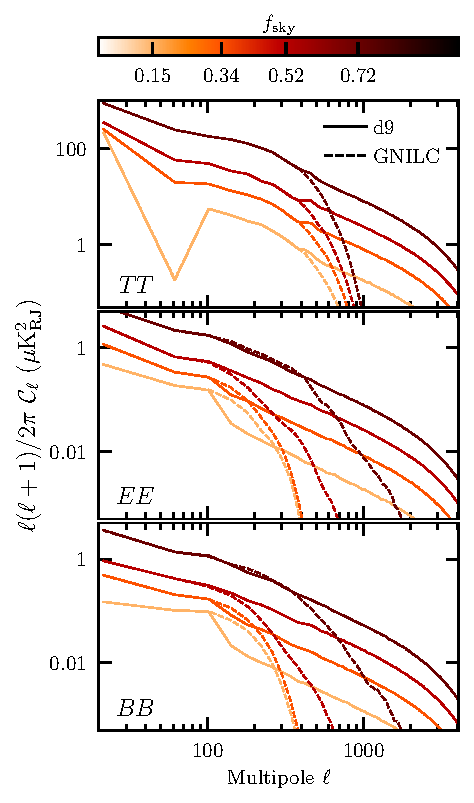
\includegraphics{paper_spectra_by_field_NSIDE2048.pdf}
%     \caption{This figure compares the power spectra of the \dnine{} model (solid lines) and the input GNILC map (dashed lines) when computed on the \texttt{GAL015}, \texttt{GAL034}, \texttt{GAL052}, and \texttt{GAL072} Galactic masks.}
%     \label{fig:spectra_by_field}
% \end{figure}

% \begin{figure}
%     \centering
%     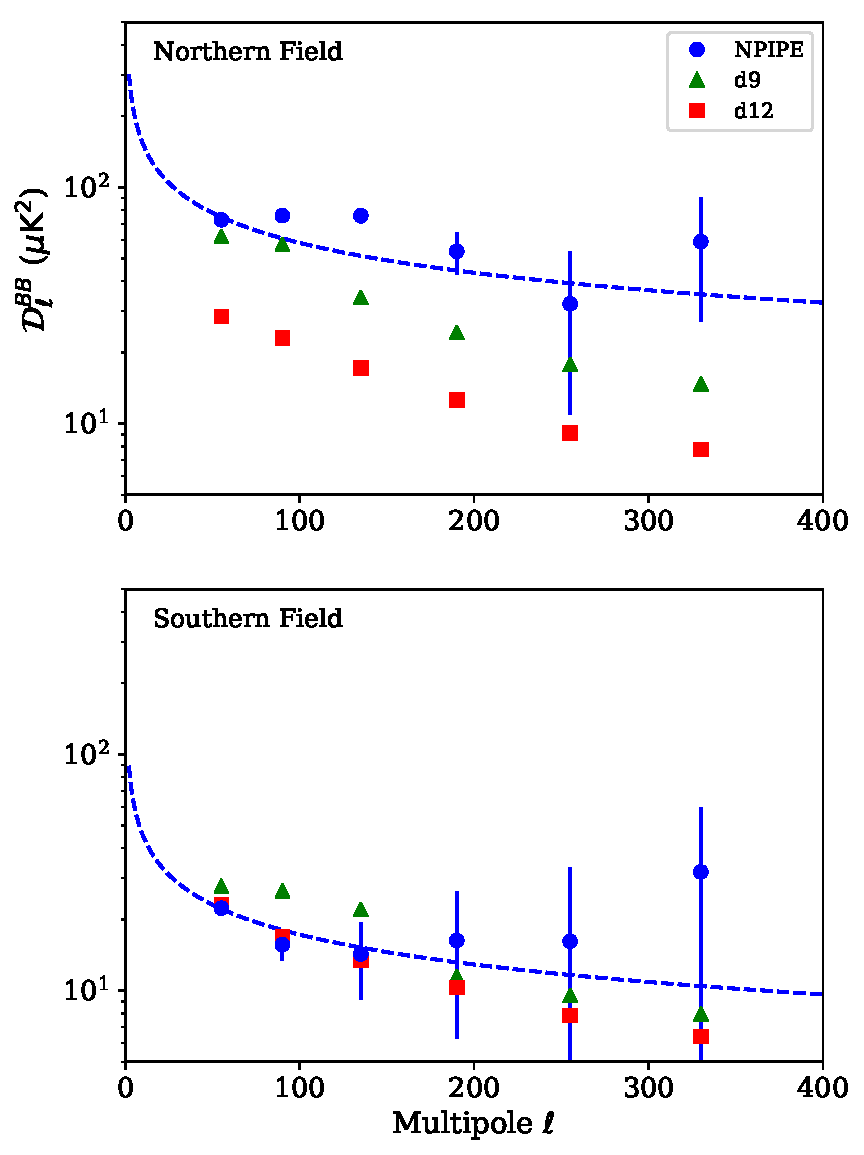
\includegraphics[width=0.48\textwidth]{figures/smallfield_power.pdf}
%     \caption{The binned $BB$ power spectra from the 353~GHz NPIPE half-ring split maps and dust model maps \texttt{d9} and \texttt{d12}. The model maps are integrated with a 353~GHz delta bandpass and the NPIPE data maps are color-corrected (i.e. scaled by a factor of 0.92) to the same single frequency. The dashed lines indicate the best-fit of the fixed-index power law ($\mathcal{D}_\ell^{BB} = A^{BB} \big( l/80 \big)^{\alpha^{BB}+2}$ where $\alpha^{BB} = -2.42$) to the NPIPE data points, which is largely driven by the first two band powers. Note that we only show the \texttt{d9} results as this model is identical to \texttt{d10} at 353~GHz.}
%     \label{fig:smallfield_power}
% \end{figure}

% \subsubsection{Small Field Power Analysis} 

% \textbf{Kenny:} To compare the small-scale performances of the latest PySM dust models \texttt{d9}, \texttt{d10} and \texttt{d12} with real data, we mainly follow the analysis method described in \cite{planck2014-XXX} to examine the model behaviors. We first use a HEALPix grid with $\texttt{nside} = 8$ to divide the full sky into 768 patches. At the center of each patch, we create a 400-square-degree circular mask with its edge tapered by a $2^\circ$ FWHM Gaussian (resulting in $f_{\rm sky} \approx 0.008$), and apply such a mask to the mean-subtracted dust model and NPIPE half-ring split maps at 353~GHz. We then use \texttt{anafast} to compute the binned $BB$ auto-spectra of the masked model maps at $\ell = 55,90,135,190,255,330$ with $\Delta \ell = 30$, and scale them to be the full-sky $\mathcal{D}_\ell^{BB}$ by dividing the apodization mask integral squared. For the masked NPIPE data maps, we instead compute cross-spectrum from the two split maps to minimize the noise correlation. The representative results from two selected circular fields at $|b| > 30^\circ$ of the northern and southern Galactic hemispheres are shown in Fig.~\ref{fig:smallfield_power}. (\textbf{Kenny:} this analysis uses anafast - contradicts with the NaMaster stated above?)

% We would like to explore whether the PySM models can reproduce the dust $BB$ power spectrum's amplitude and steepness over $\ell$ in reality, especially in those high Galactic latitude small fields. We therefore compute the low-$\ell$ averaged $\mathcal{D}_\ell^{BB}$ (over $\ell = 55, 90$) and the high-$\ell$ averaged $\mathcal{D}_\ell^{BB}$ (over $\ell = 135, 190, 255, 330$) of each small field for the model and NPIPE maps, and we present the results in scatter plots in Fig.~\ref{fig:smallfield_power_all}. It turns out that the amplitude of the \texttt{d12} model is in general smaller than the preference of NPIPE data, as a large fraction of the d12 data points cluster around the lower-left corner of the plot. The wider span of the \texttt{d12} data points along the vertical direction also implies the model spectrum steepness varies more over the sky. In contrast, the \texttt{d9}/\texttt{d10} data points are fairly compatible with the NPIPE results, although they predict slightly steeper power spectra. If we define the ratio of the low-$\ell$ mean value to the high-$\ell$ mean value as a proxy for describing the spatial power change across the modulation scale, while the perfect fixed-index power law $\mathcal{D}_\ell^{BB} \propto \ell^{-0.42}$ yields a value of $\approx 1.60$, the NPIPE maps give $1.65 \pm 0.68$ and the \texttt{d9}/\texttt{d10} (\texttt{d12}) model map gives $2.37 \pm 0.77$ ($2.24 \pm 0.87$) over sky patches with $|b| > 30^\circ$.

% \begin{figure}
%     \centering
%     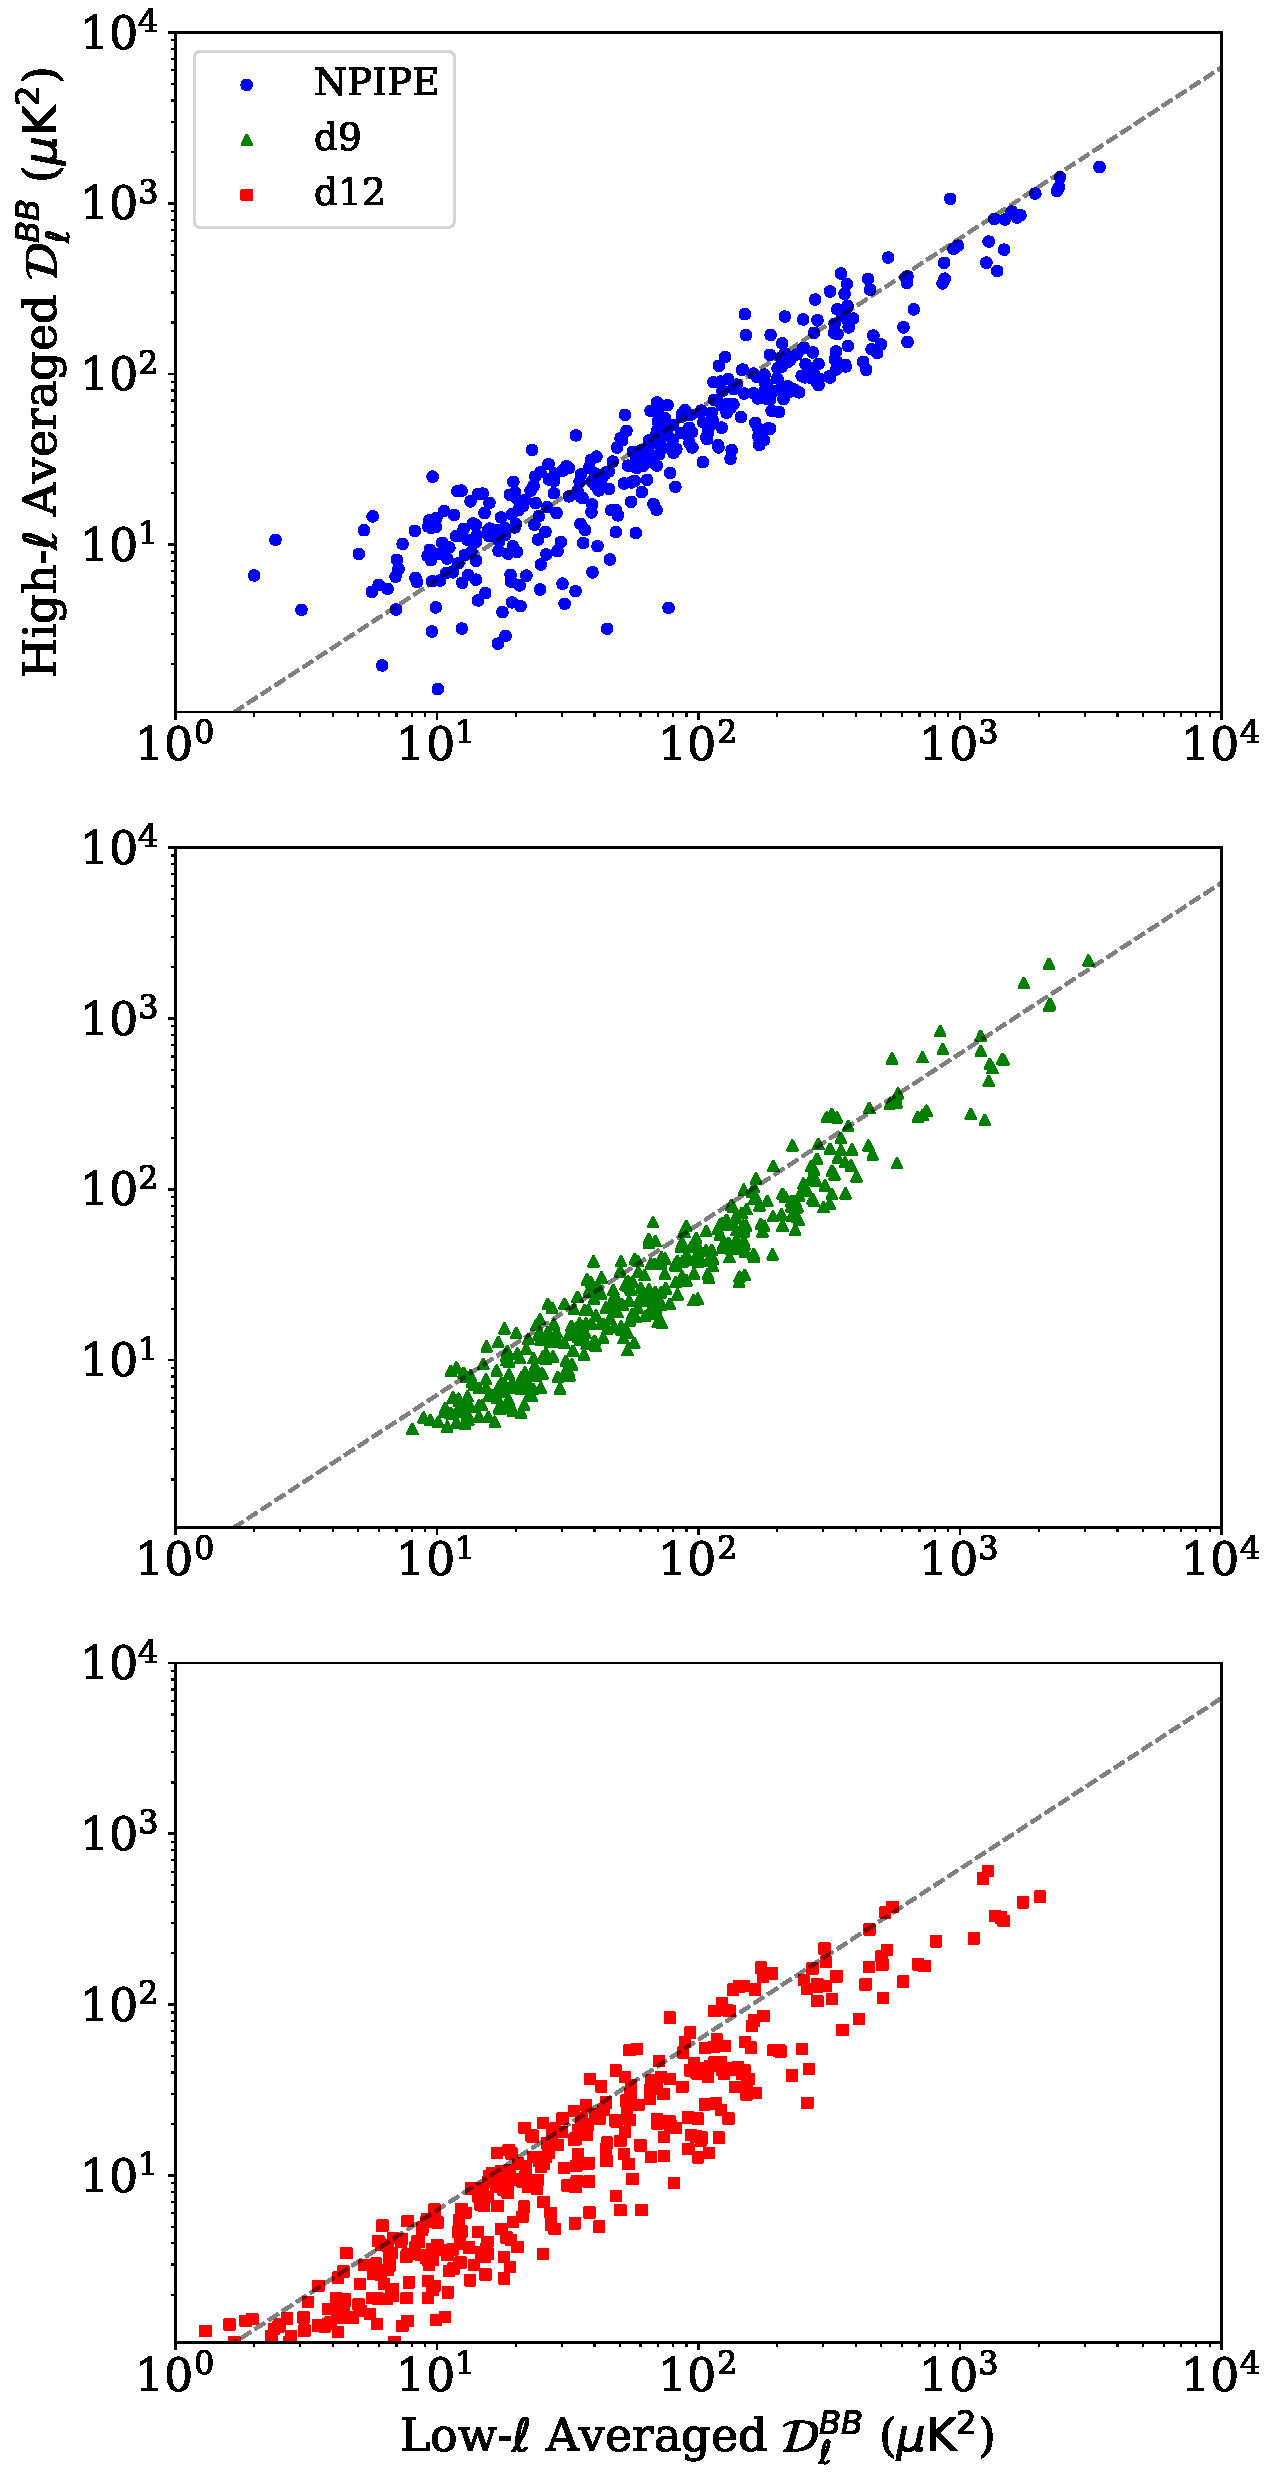
\includegraphics[width=0.48\textwidth]{figures/all2_lhmean.pdf}
%     \caption{Scatter plots of the mean of the first two $BB$ band powers versus the mean of the last four $BB$ band powers shown in Fig.~\ref{fig:smallfield_power}. Each data point represents the results from a circular sky patches with $|b| > 30^\circ$. Dashed reference lines indicating $\mathcal{D}_\ell^{BB} \propto \ell^{-0.42}$ are added to the plots. This power law in fact comes from the analysis of several larger sky regions ($f_\text{sky} = 0.3 \; \text{to} \; 0.8$) by \cite{planck2014-XXX}, but the small-field NPIPE data points, which spread out when the dust amplitude is small presumably due to map noise, are consistent with it as well. Another important feature is that the trends of the \texttt{d9} and \texttt{d12} data points are lower than that of the NPIPE in these log-log plots, implying that the model spectra are steeper.}
%     \label{fig:smallfield_power_all}
% \end{figure}

% \subsubsection{BICEP / Keck} \label{sec:bkspt_spectra}

% \textbf{Ben:} The current upper limit on the tensor-to-scalar ratio is set by a combination of BICEP / Keck (BK), Planck, and WMAP data: $r < 0.036~(95\%)$ \citep{Ade:2021}. Over the next few years, a collaborative effort between the South Pole Telescope (SPT) and BICEP / Keck will combine high-resolution SPT-3G observations with BK observations in order to ``delens'' the observed CMB B-modes, and further constrain $r$. Therefore, there will be continued interest in simulating Galactic foregrounds on this particular patch of sky.

% In Figure~\ref{fig:d1d9_bkpatch} we compare the BB power spectrum of the new \dnine{} model with the original PySM \done{} model, the GNILC input map, and the maximum likelihood dust model in this patch of sky determined from a combination of BK, Planck and WMAP data \citep{Ade:2021}. Model \done{} clearly has excess dust BB power compared to the measured amplitude in this patch of sky, which has been known for some time. This is somewhat ameliorated in model \dnine{}, primarily due to the steeper spectral tilt of the \dnine{} model leading to a factor of $\sim 10$ decrease in power relative to \done{} by multipoles of $\ell \gtrsim 300$. At larger scales of $\ell \lesssim 50$ both the \done{} and \dnine{} models are dominated by the underlying GNILC template, rather than the simulated small scale realizations, and so the mismatch in amplitude between the BK maximum likelihood model and our templates is most likely due to residual noise in the GNILC template. Indeed, most of the constraining power on dust BB power in Ref~\cite{Ade:2021} is driven by BK observations at 220\,GHz, which are not used to inform our model. 

% One may argue that the amplitude and spectral tilt of the \dnine{} model clearly disagree with existing observations in the BK patch of sky. While this is true, it is beyond the scope of this work to provide full sky simulations that guarantee consistency with all sets of full sky and partial sky observations. Indeed, the use of power spectrum-based techniques requires a certain amount of global averaging of power spectrum parameters that are in fact known to vary across the sky \cite{planck2016-l04}. For example, while the dust amplitude can be modulated by the use of a large scale template, the spectral tilt has to be fixed to a single value for the full sky, which is not realistic. 

% \begin{figure}[ht]
%     \centering
%     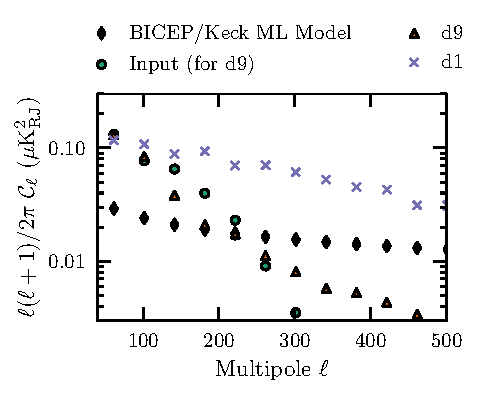
\includegraphics{paper_BK_patch.pdf}
%     \caption{This figure shows the BB power spectra of the \done{} (crosses), \dnine{} (triangles), and varres GNILC map (circles), compared to the maximum likelihood BK dust model (black diamonds) derived from a combination of WMAP and Planck with BICEP / Keck data up to the 2018 observing season. Note that in order to make a meaningful comparison between the bandpowers calculated from maps and the theory curve, we first convolve the theory spectrum with the mode-coupling matrix and then compute the decoupled bandpowers by applying the inverted binned coupling matrix.}
%     \label{fig:d1d9_bkpatch}
% \end{figure}

% \subsubsection{Map level validation}
% %In this section, we present a map-level validation of the PySM dust models \dnine{}, {\tt d11}, {\tt d12} models against the Planck third data release (PR3) \cite{}.
% \textbf{Elisa}: In this section, we compare at the map level, Planck third data release PR3 \cite{planck2016-l03}) and PySM dust models \dnine{}, {\tt d11}, {\tt d12} models. We study how well the modeled intensity $I$ and polarized intensity $P = \sqrt{U^2 + Q^2}$ match the observations on three selected $16.7^\circ \times 16.7^\circ$ patches of the sky, at 353~GHz. Here, we focus on two local patches: close to the Galactic plane ($[l,b] =[180^\circ,-10^\circ]$) and, centered on the Bicep / Keck field ($[l,b] =[318^\circ,-61^\circ]$).
% Similar to Section~\ref{sec:sync_validation}, we integrate the dust models within the Planck passbands to enable direct comparison. For comparison of intensity maps, we subtract a Wiener-filtered CMB temperature anisotropies map from SMICA and adjust the zero level of the PR3 data to that of the simulated map over regions of faint dust intensity on the sky.
% The mask used to adjust the zero levels is shown in figure \ref{fig:mask_zero_lvl_int}. These corrections are not required for comparing polarization data.
% \begin{figure}[ht!]
%     \centering
%     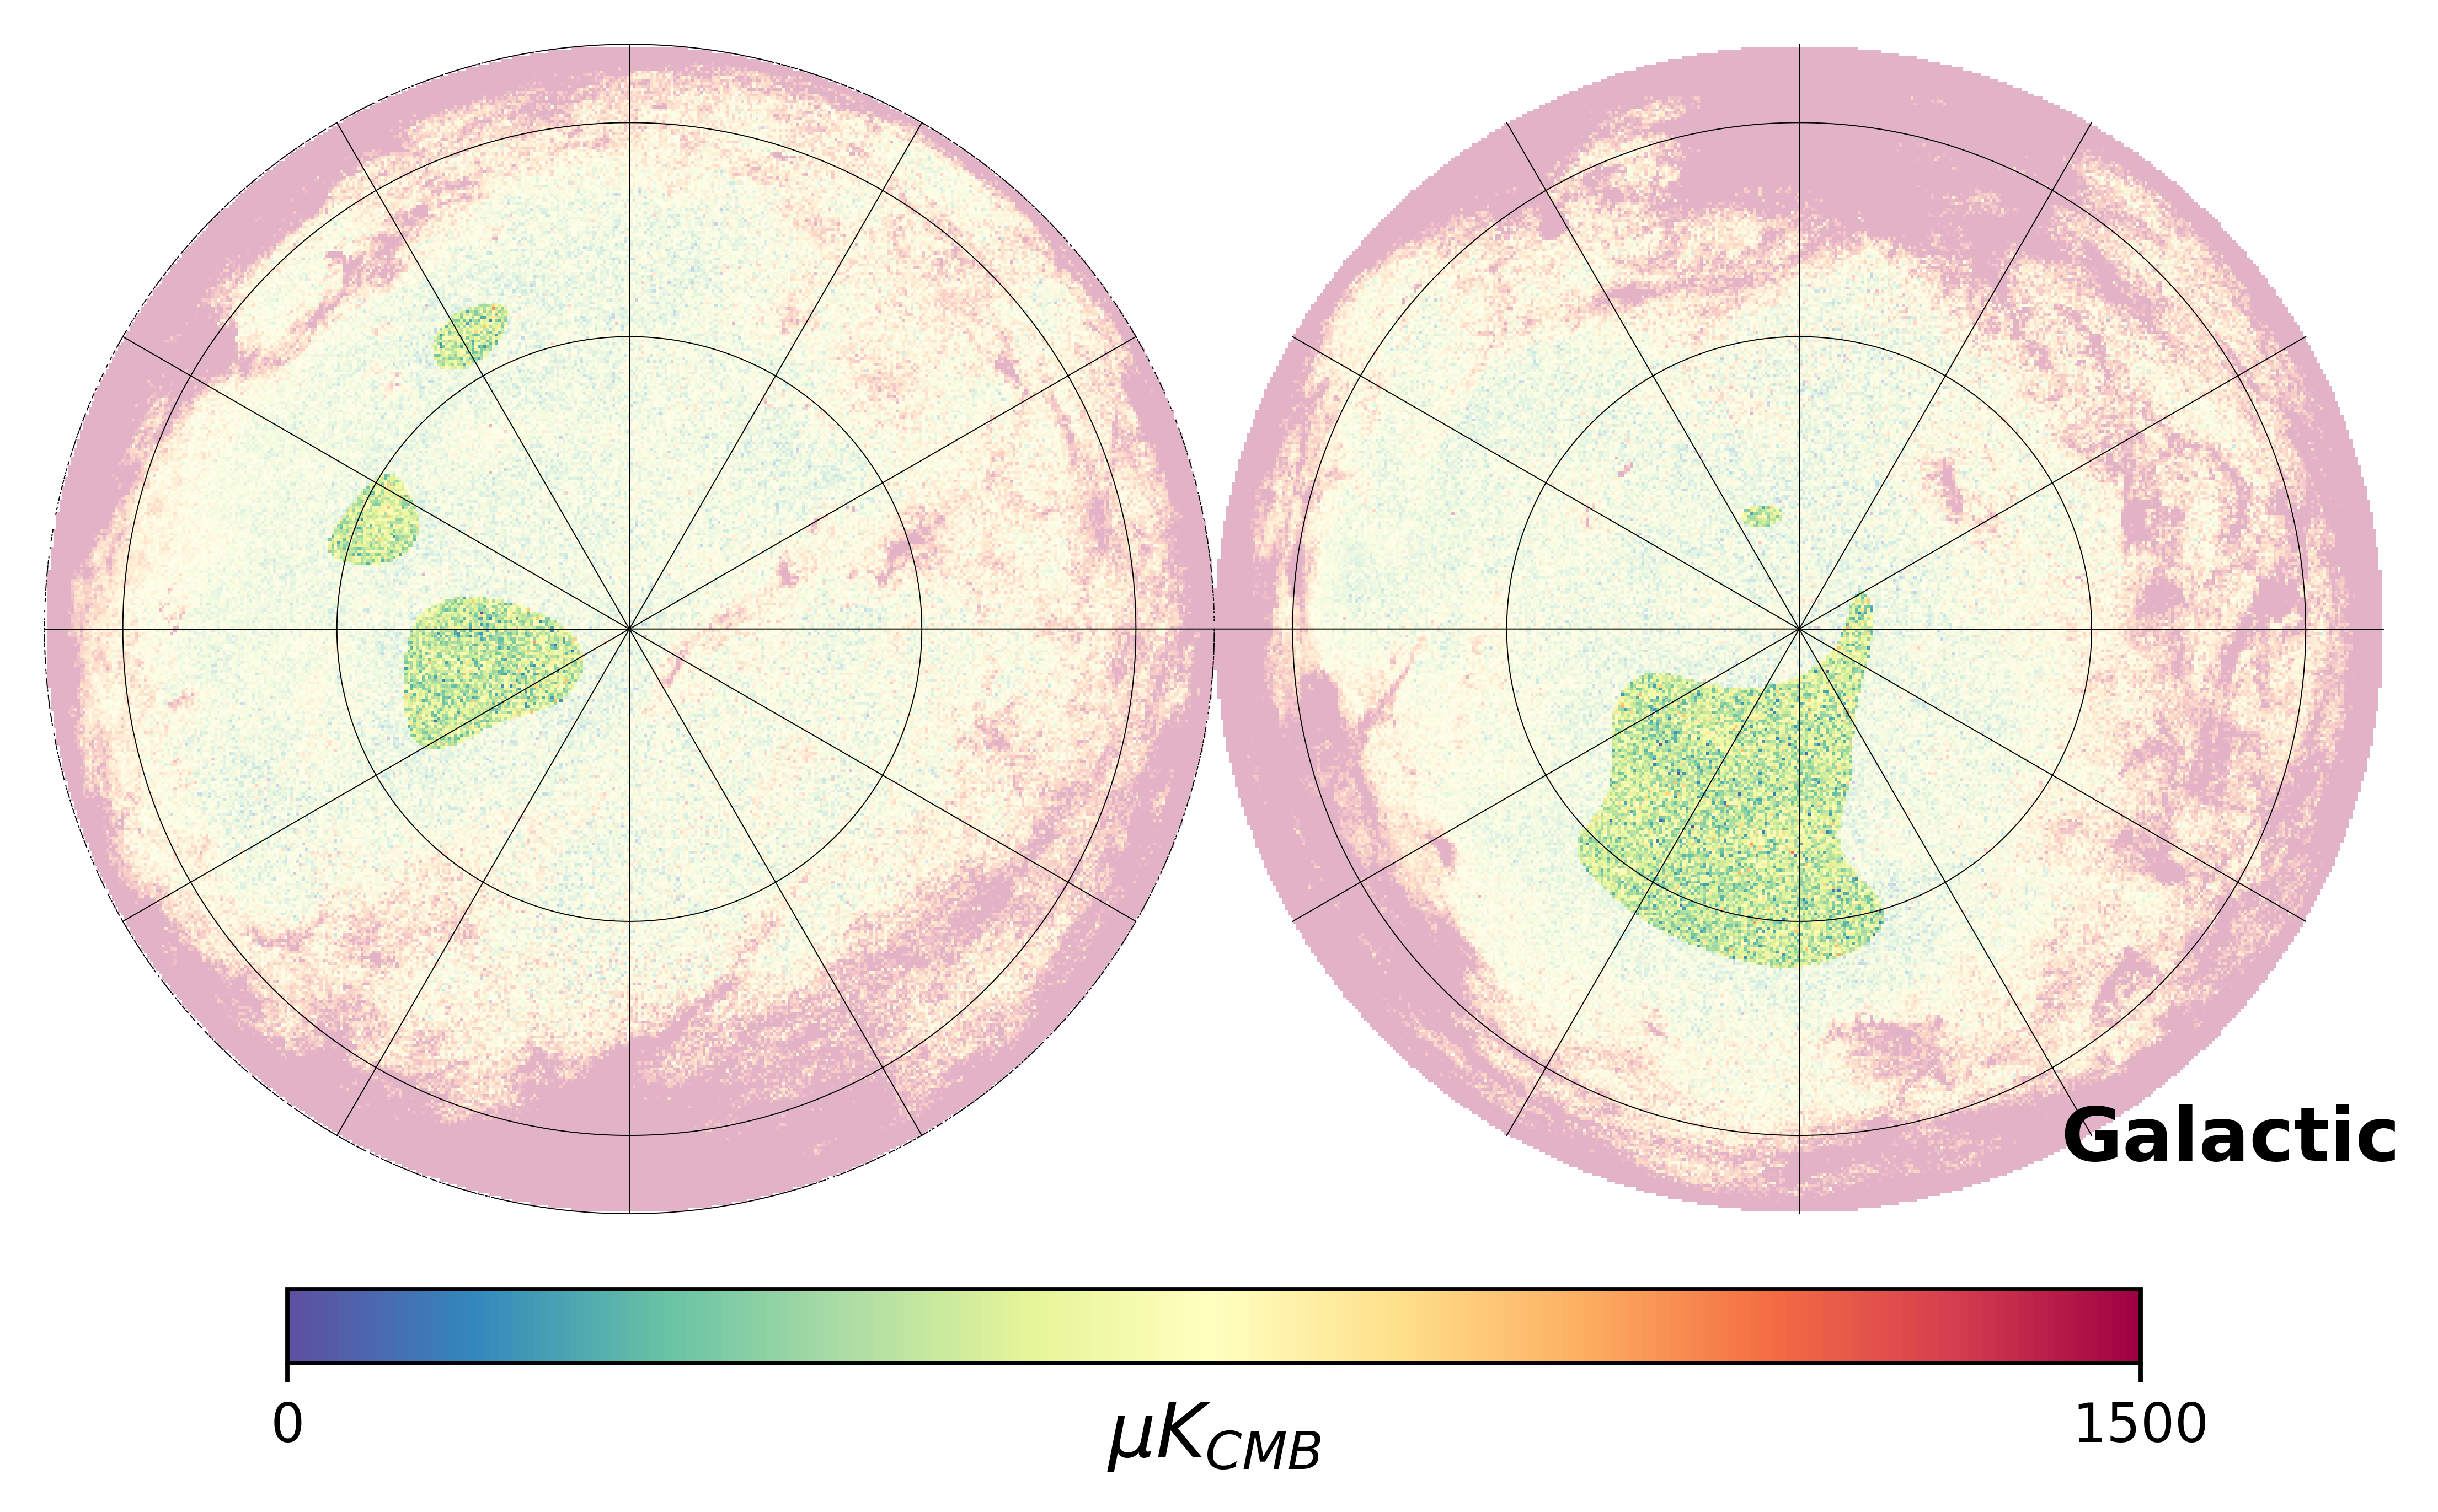
\includegraphics[width=0.48\textwidth]{figures/mask_intxPR3_zero_lvl.png}
%     \caption{Mask $\times$ PR3 intensity used to estimate the zero level of PR3 intensity. This mask is obtained by thresholding the intensity of the smoothed PR3 intensity to preserve only the regions where the dust is very low, to estimate the zero-level of the data and models.}%more details
%     \label{fig:mask_zero_lvl_int}
% \end{figure}

% \begin{figure}[ht!]
%     \centering
%     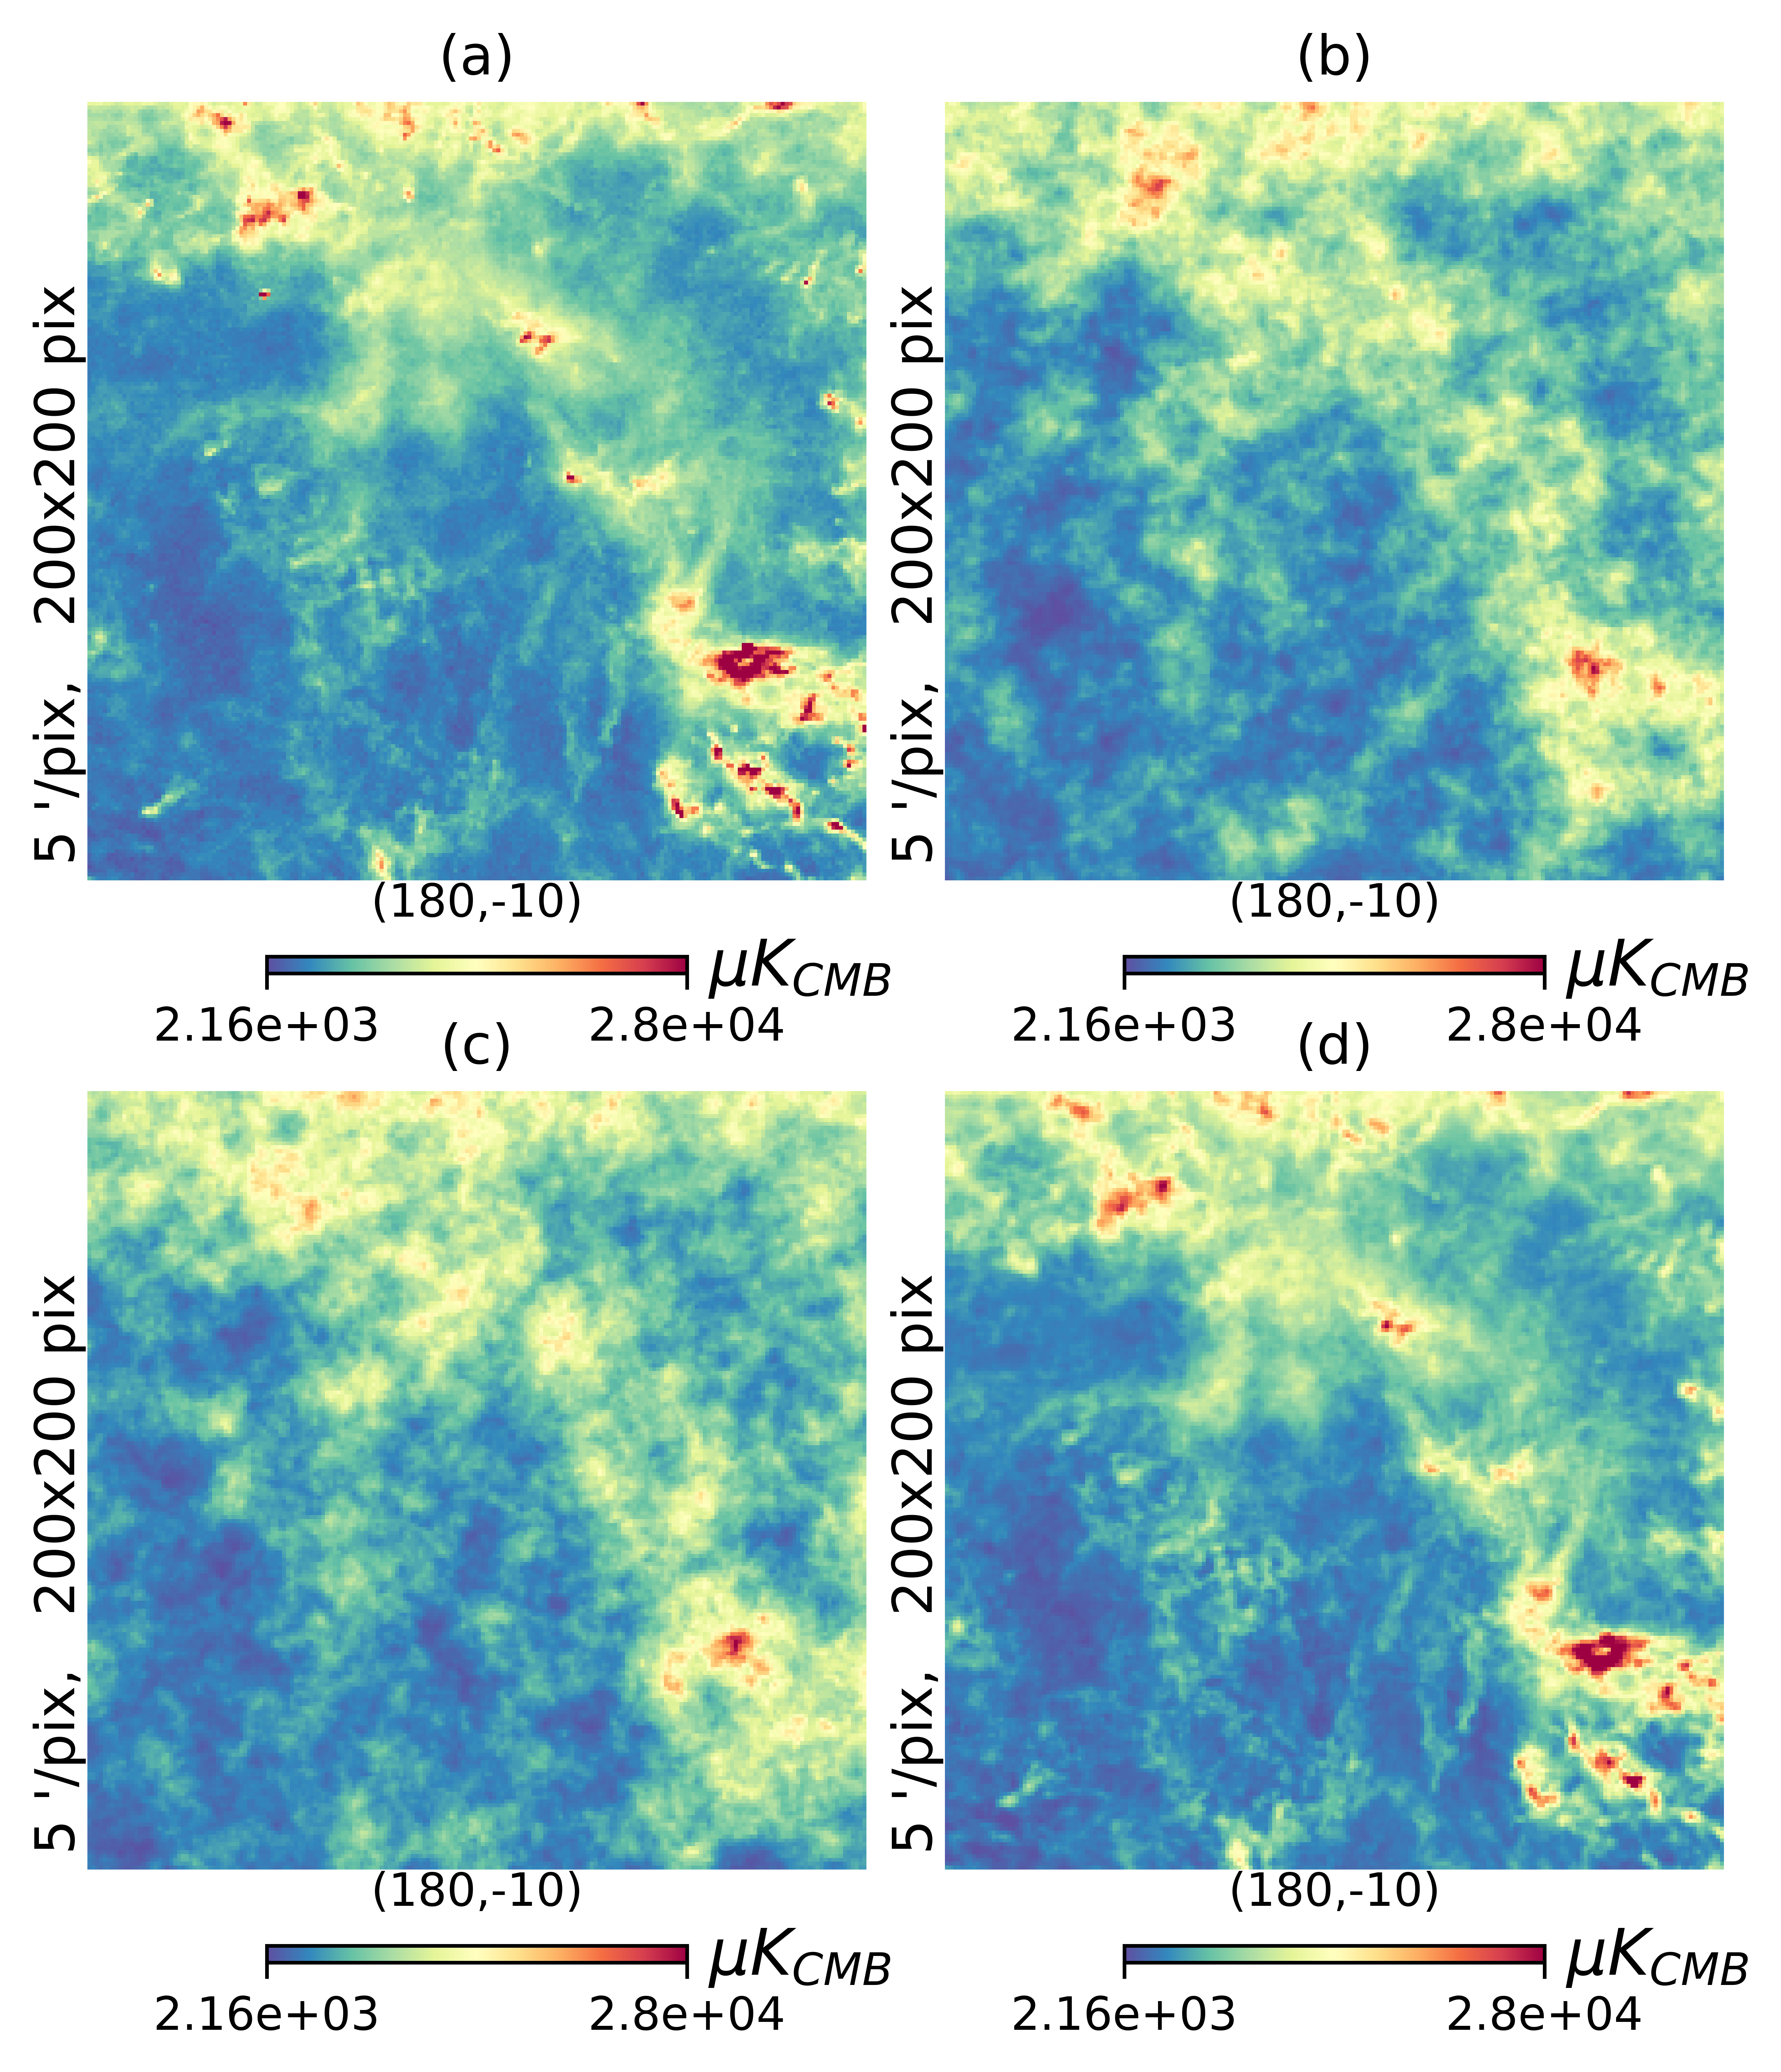
\includegraphics[width=0.48\textwidth]{figures/gal_plane_non_smooth_wo_zero_lvl.png}
% \caption{Dust intensity at 353GHz at [l = 180, b = -10] with an angular resolution of 4.94': (a) PR3 (b) d9 (c) d11 (d) d12}    
% \label{fig:353_int_gal_plane}
% \end{figure}
% % \begin{figure}
% %     \centering
% %     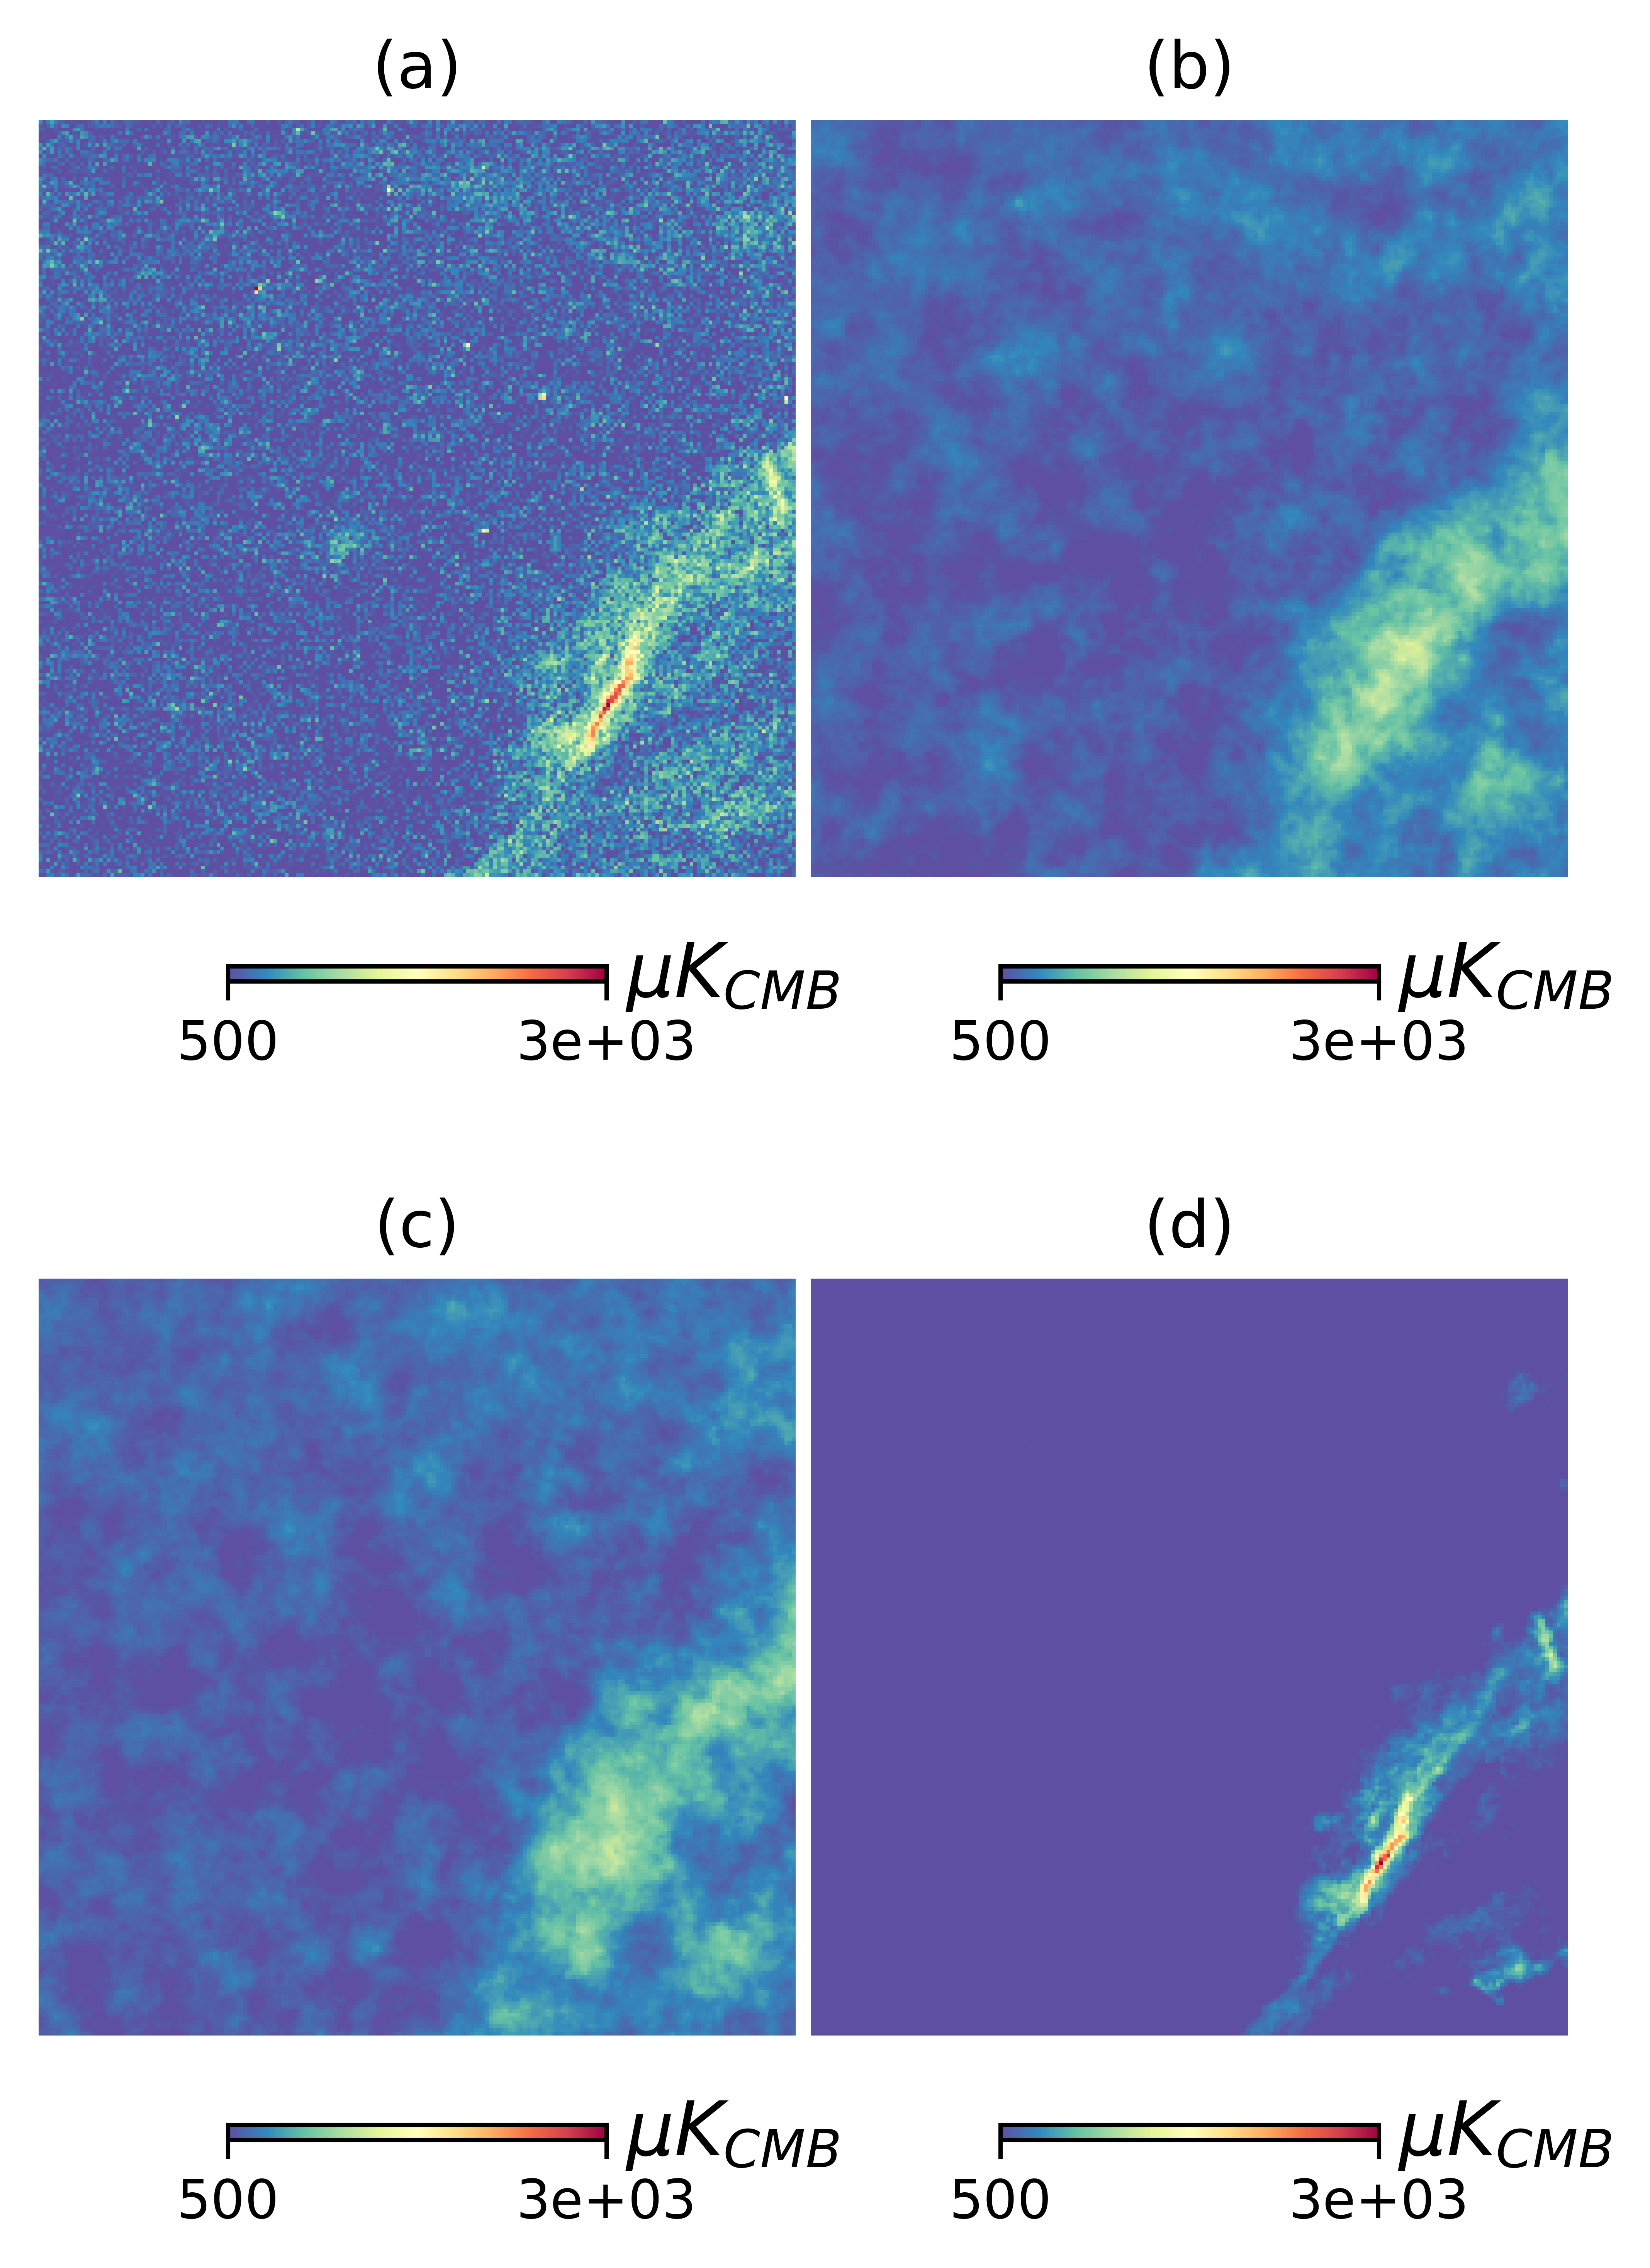
\includegraphics[scale = 0.6]{figures/NGP_non_smooth_wo_zero_lvl.png}
% %     \caption{Dust intensity at 353GHz centered at [l = 0, b = 90]: (a) PR3 (b) d9 (c) d11 (d) d12}
% %     \label{fig:353_int_NP}
% % \end{figure}
% \begin{figure}[ht!]
%     \centering
%     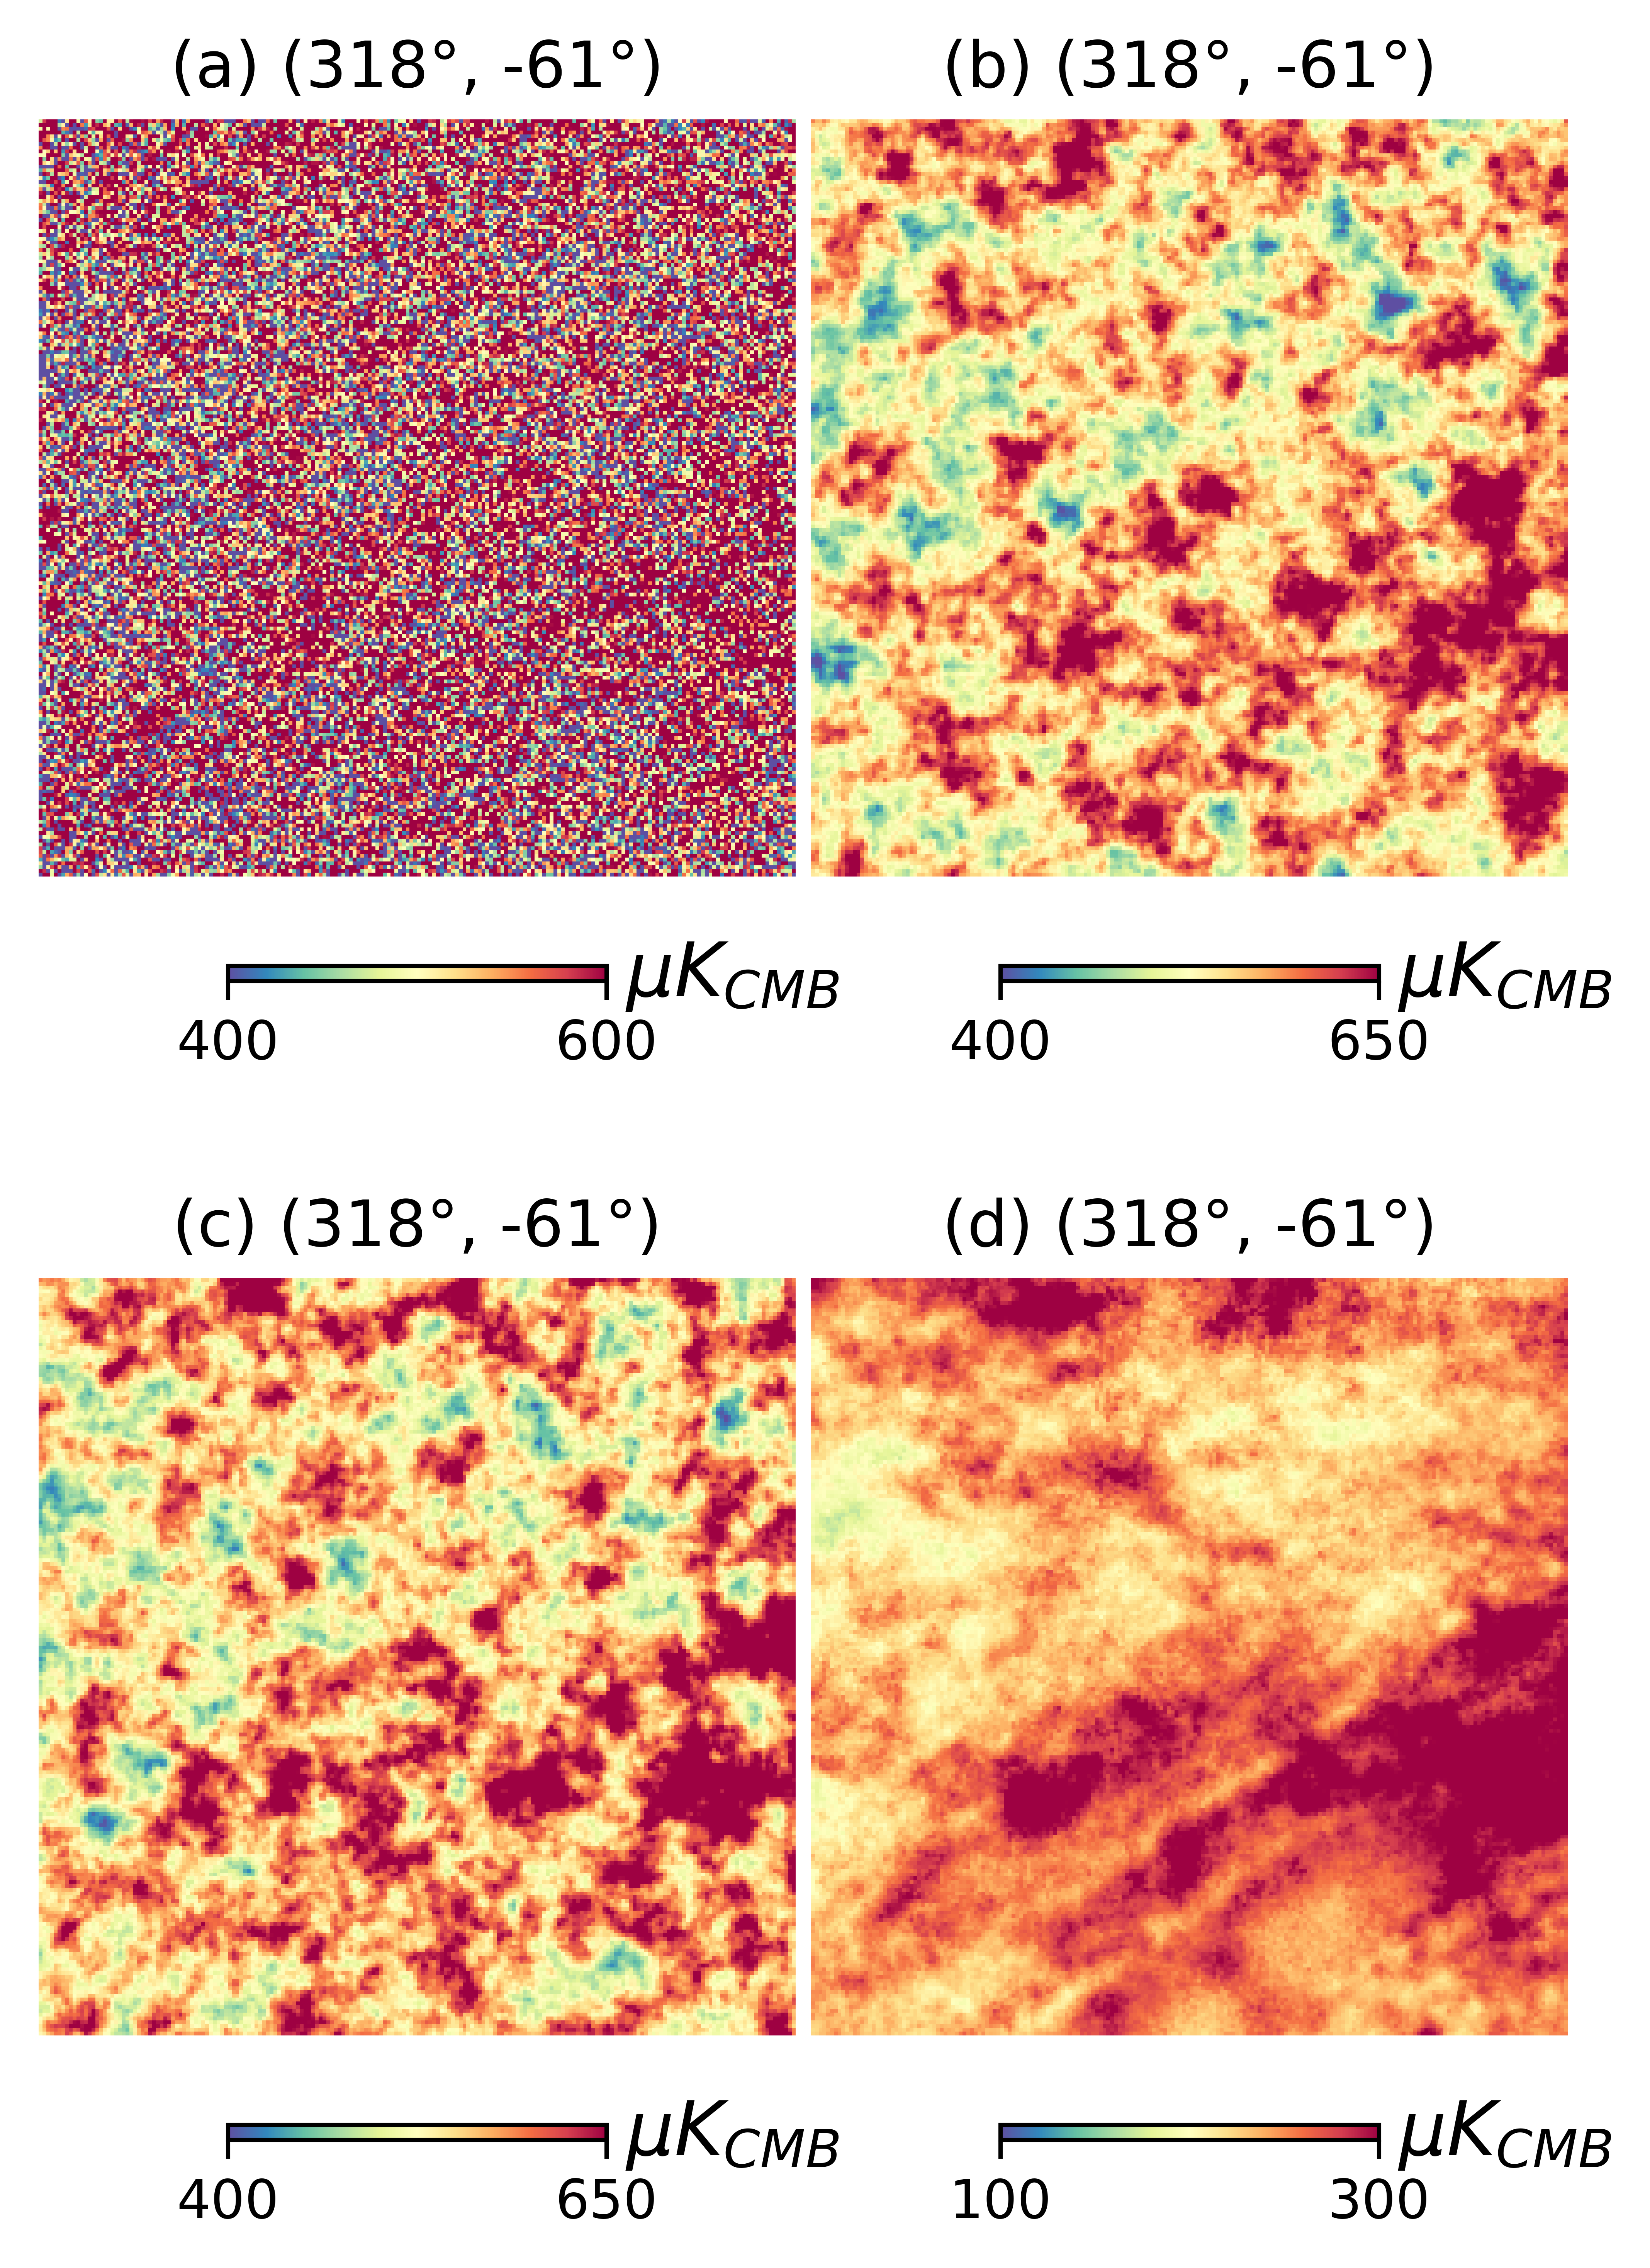
\includegraphics[width=0.48\textwidth]{figures/BK_non_smooth_wo_zero_lvl.png}
%     \caption{Dust intensity at 353GHz at [l = 318, b = -61] with an angular resolution of $4.94\arcmin$: (a) PR3 (b) d9 (c) d11 (d) d12. Here, PR3 is contaminated by CIB and extragalactic sources.}
%     \label{fig:353_int_BK}
% \end{figure}

% \begin{figure}[ht!]
%     \centering
%     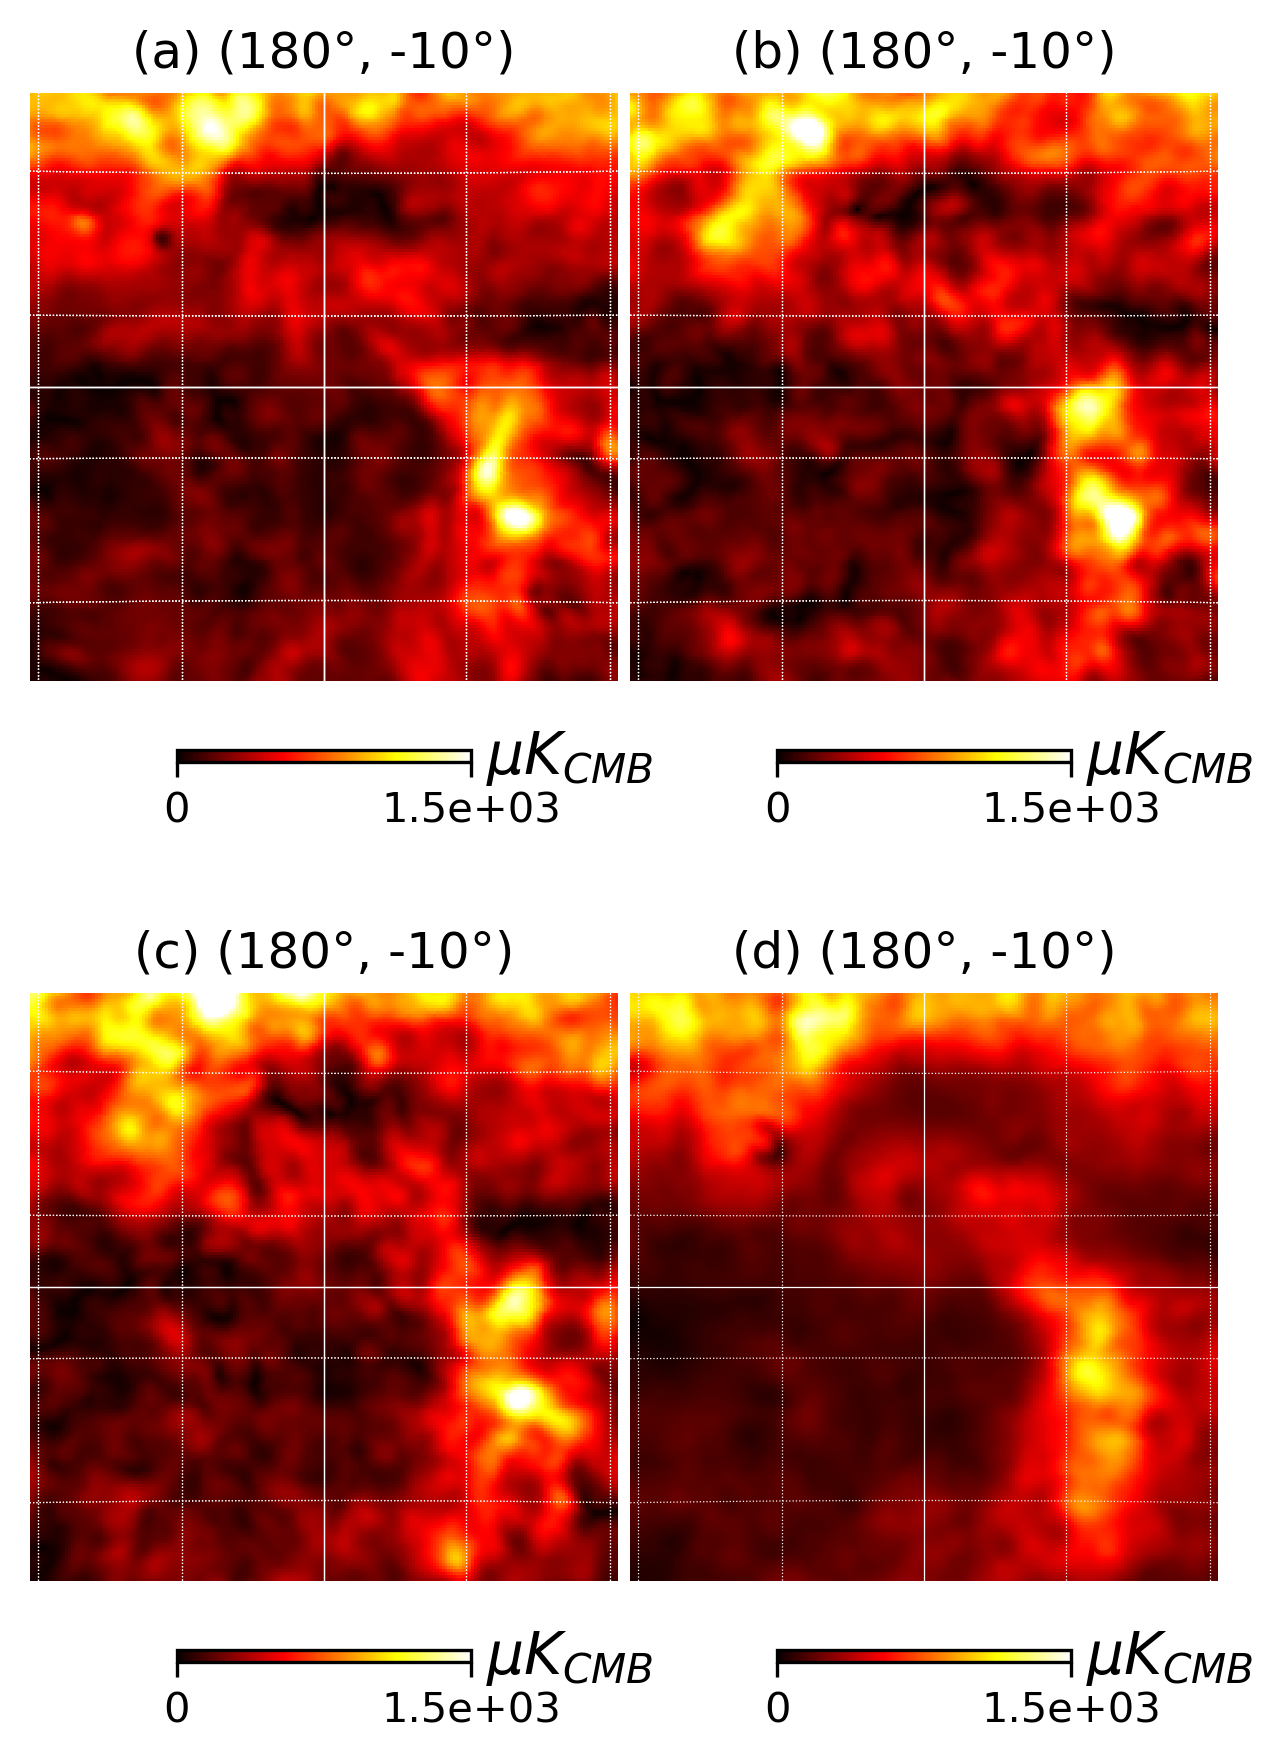
\includegraphics[width=0.48\textwidth]{figures/pol_gal_plane_smooth_30'.png}
%     \caption{Polarized dust intensity at 353GHz centered at [l = 180, b = -10] with an angular resolution of 4.94', smoothed to 30 arcmin: (a) PR3 (b) d9 (c) d11 (d) d12.}
%     \label{fig:353_pol_int_gal_plane}
% \end{figure}
% % \begin{figure}
% %     \centering
% %     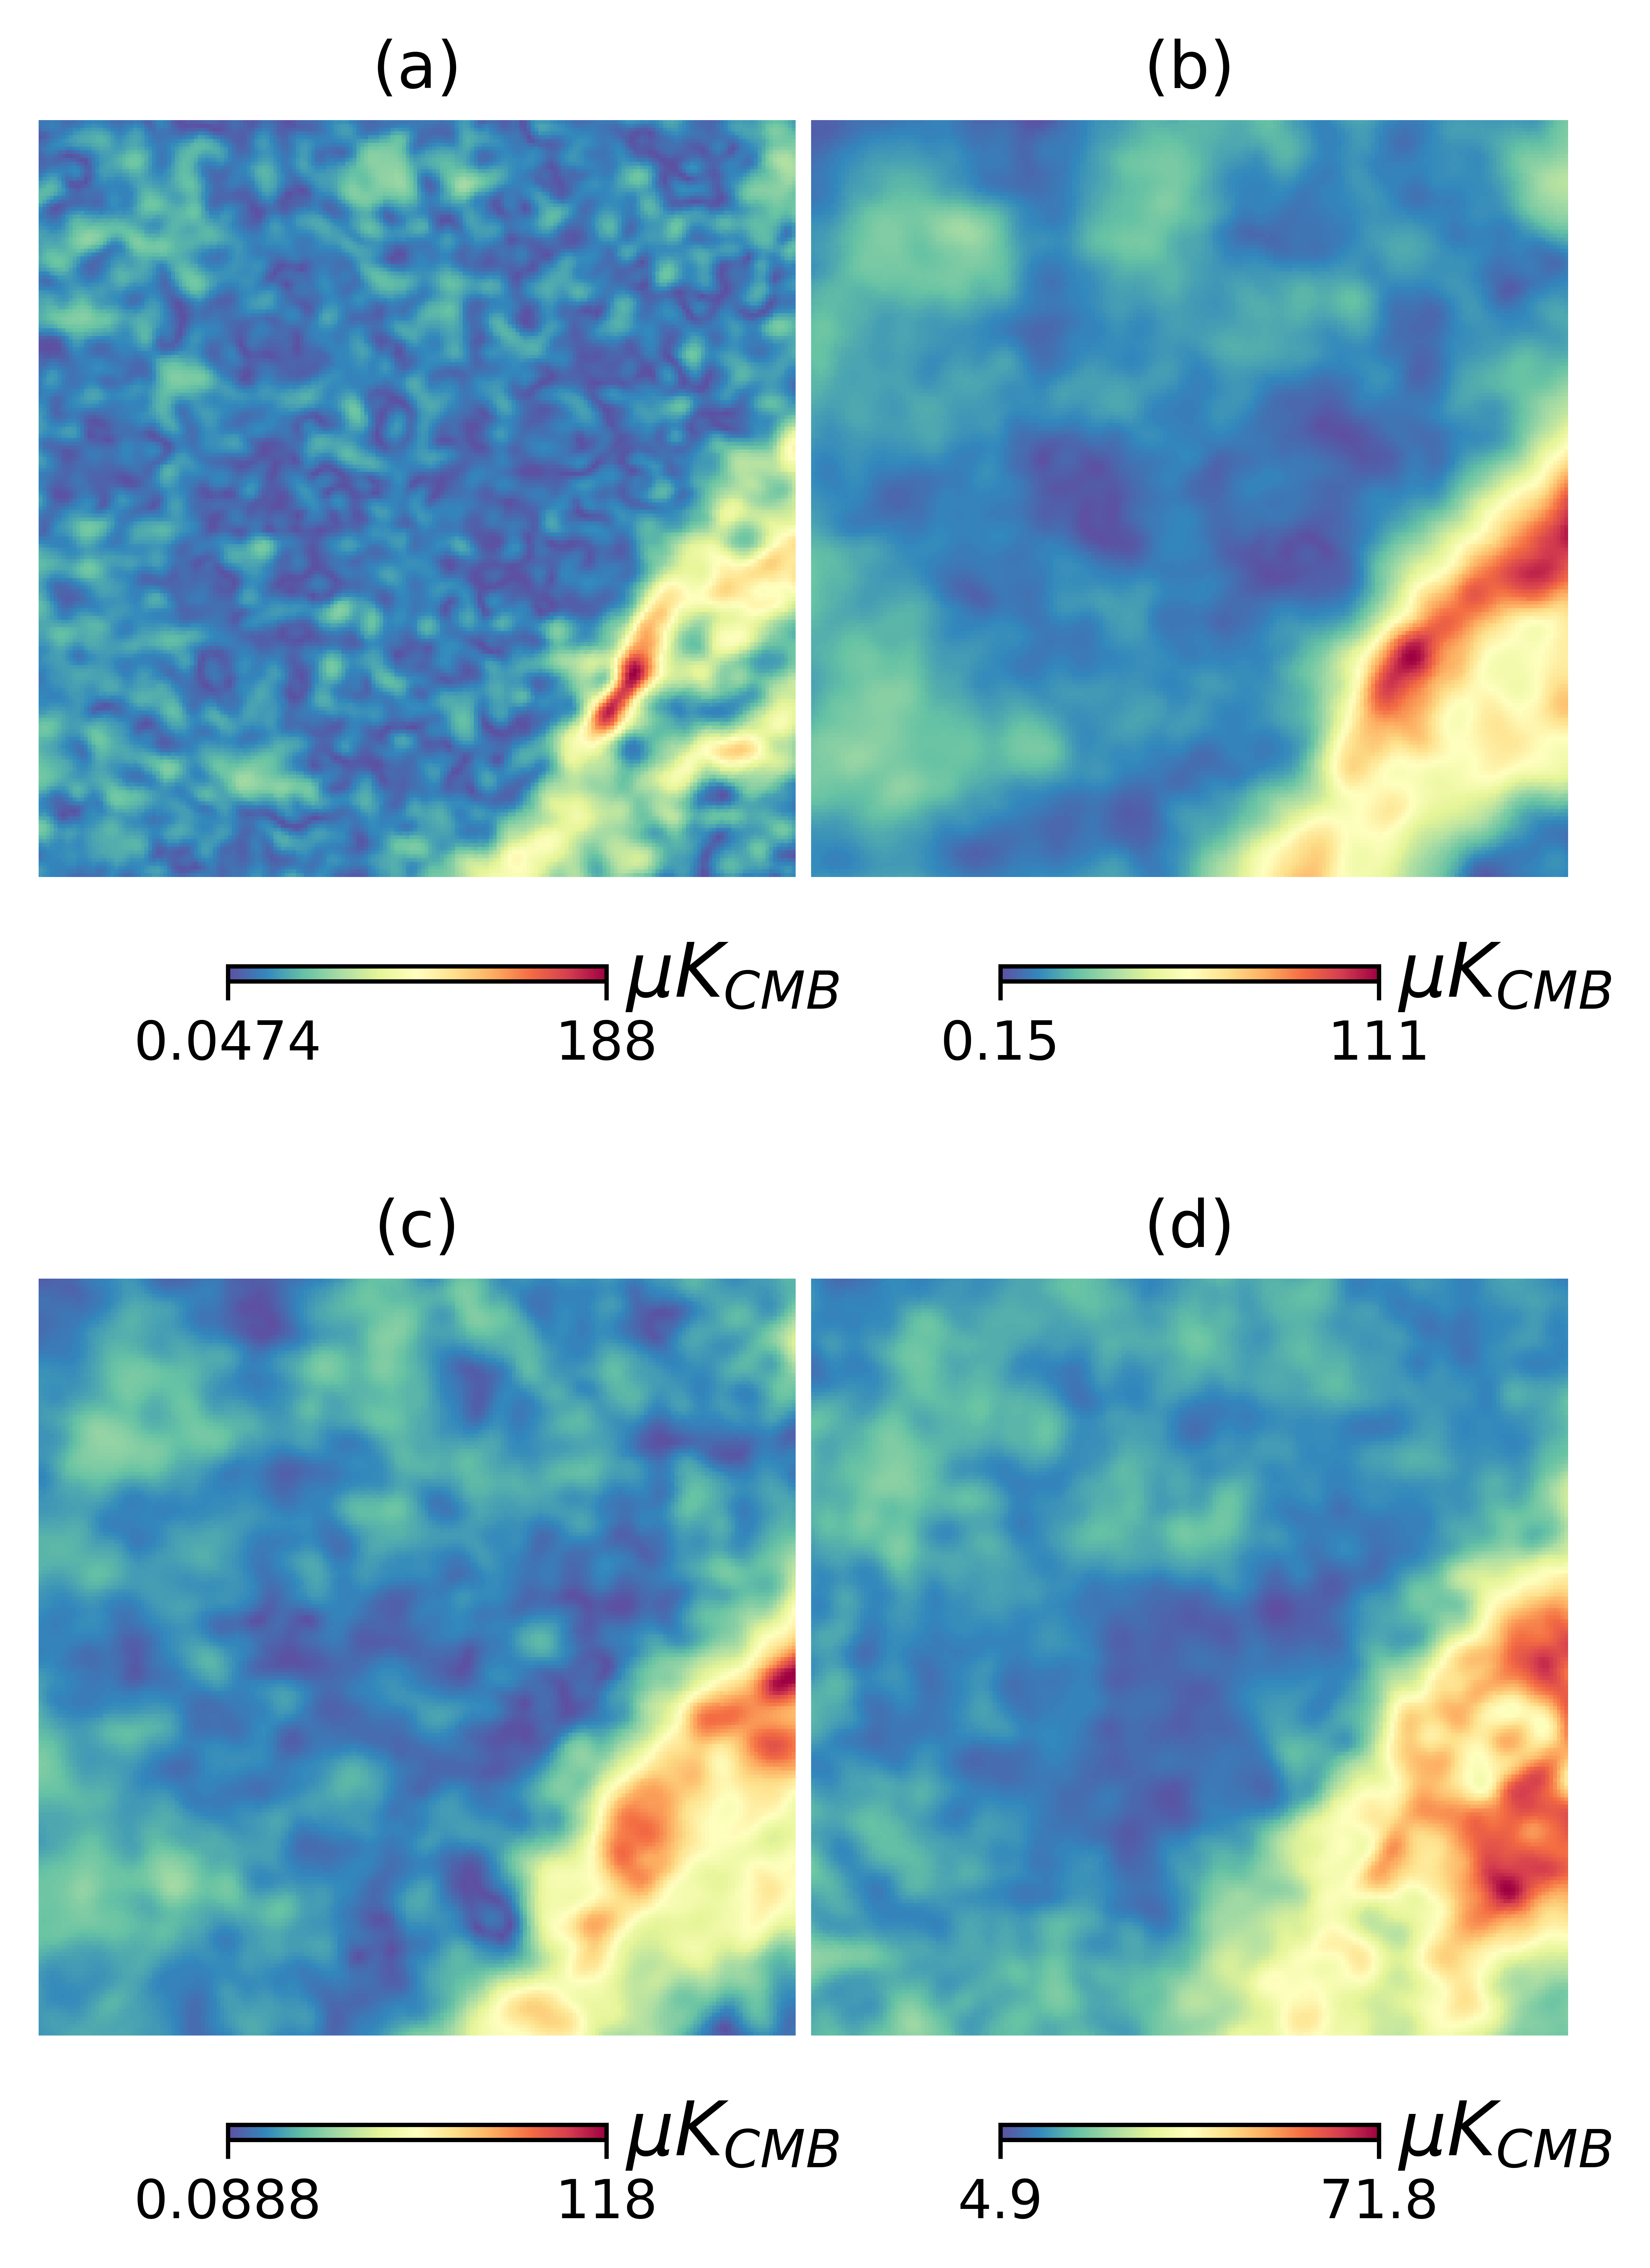
\includegraphics[scale = 0.6]{figures/pol_NGP_smooth_30'.png}
% %     \caption{Polarized dust intensity at 353GHz centered at [l = 0, b = 90].}
% %     \label{fig:353_pol_int_NGP}
% % \end{figure}

% \begin{figure}[ht!]
%     \centering
%     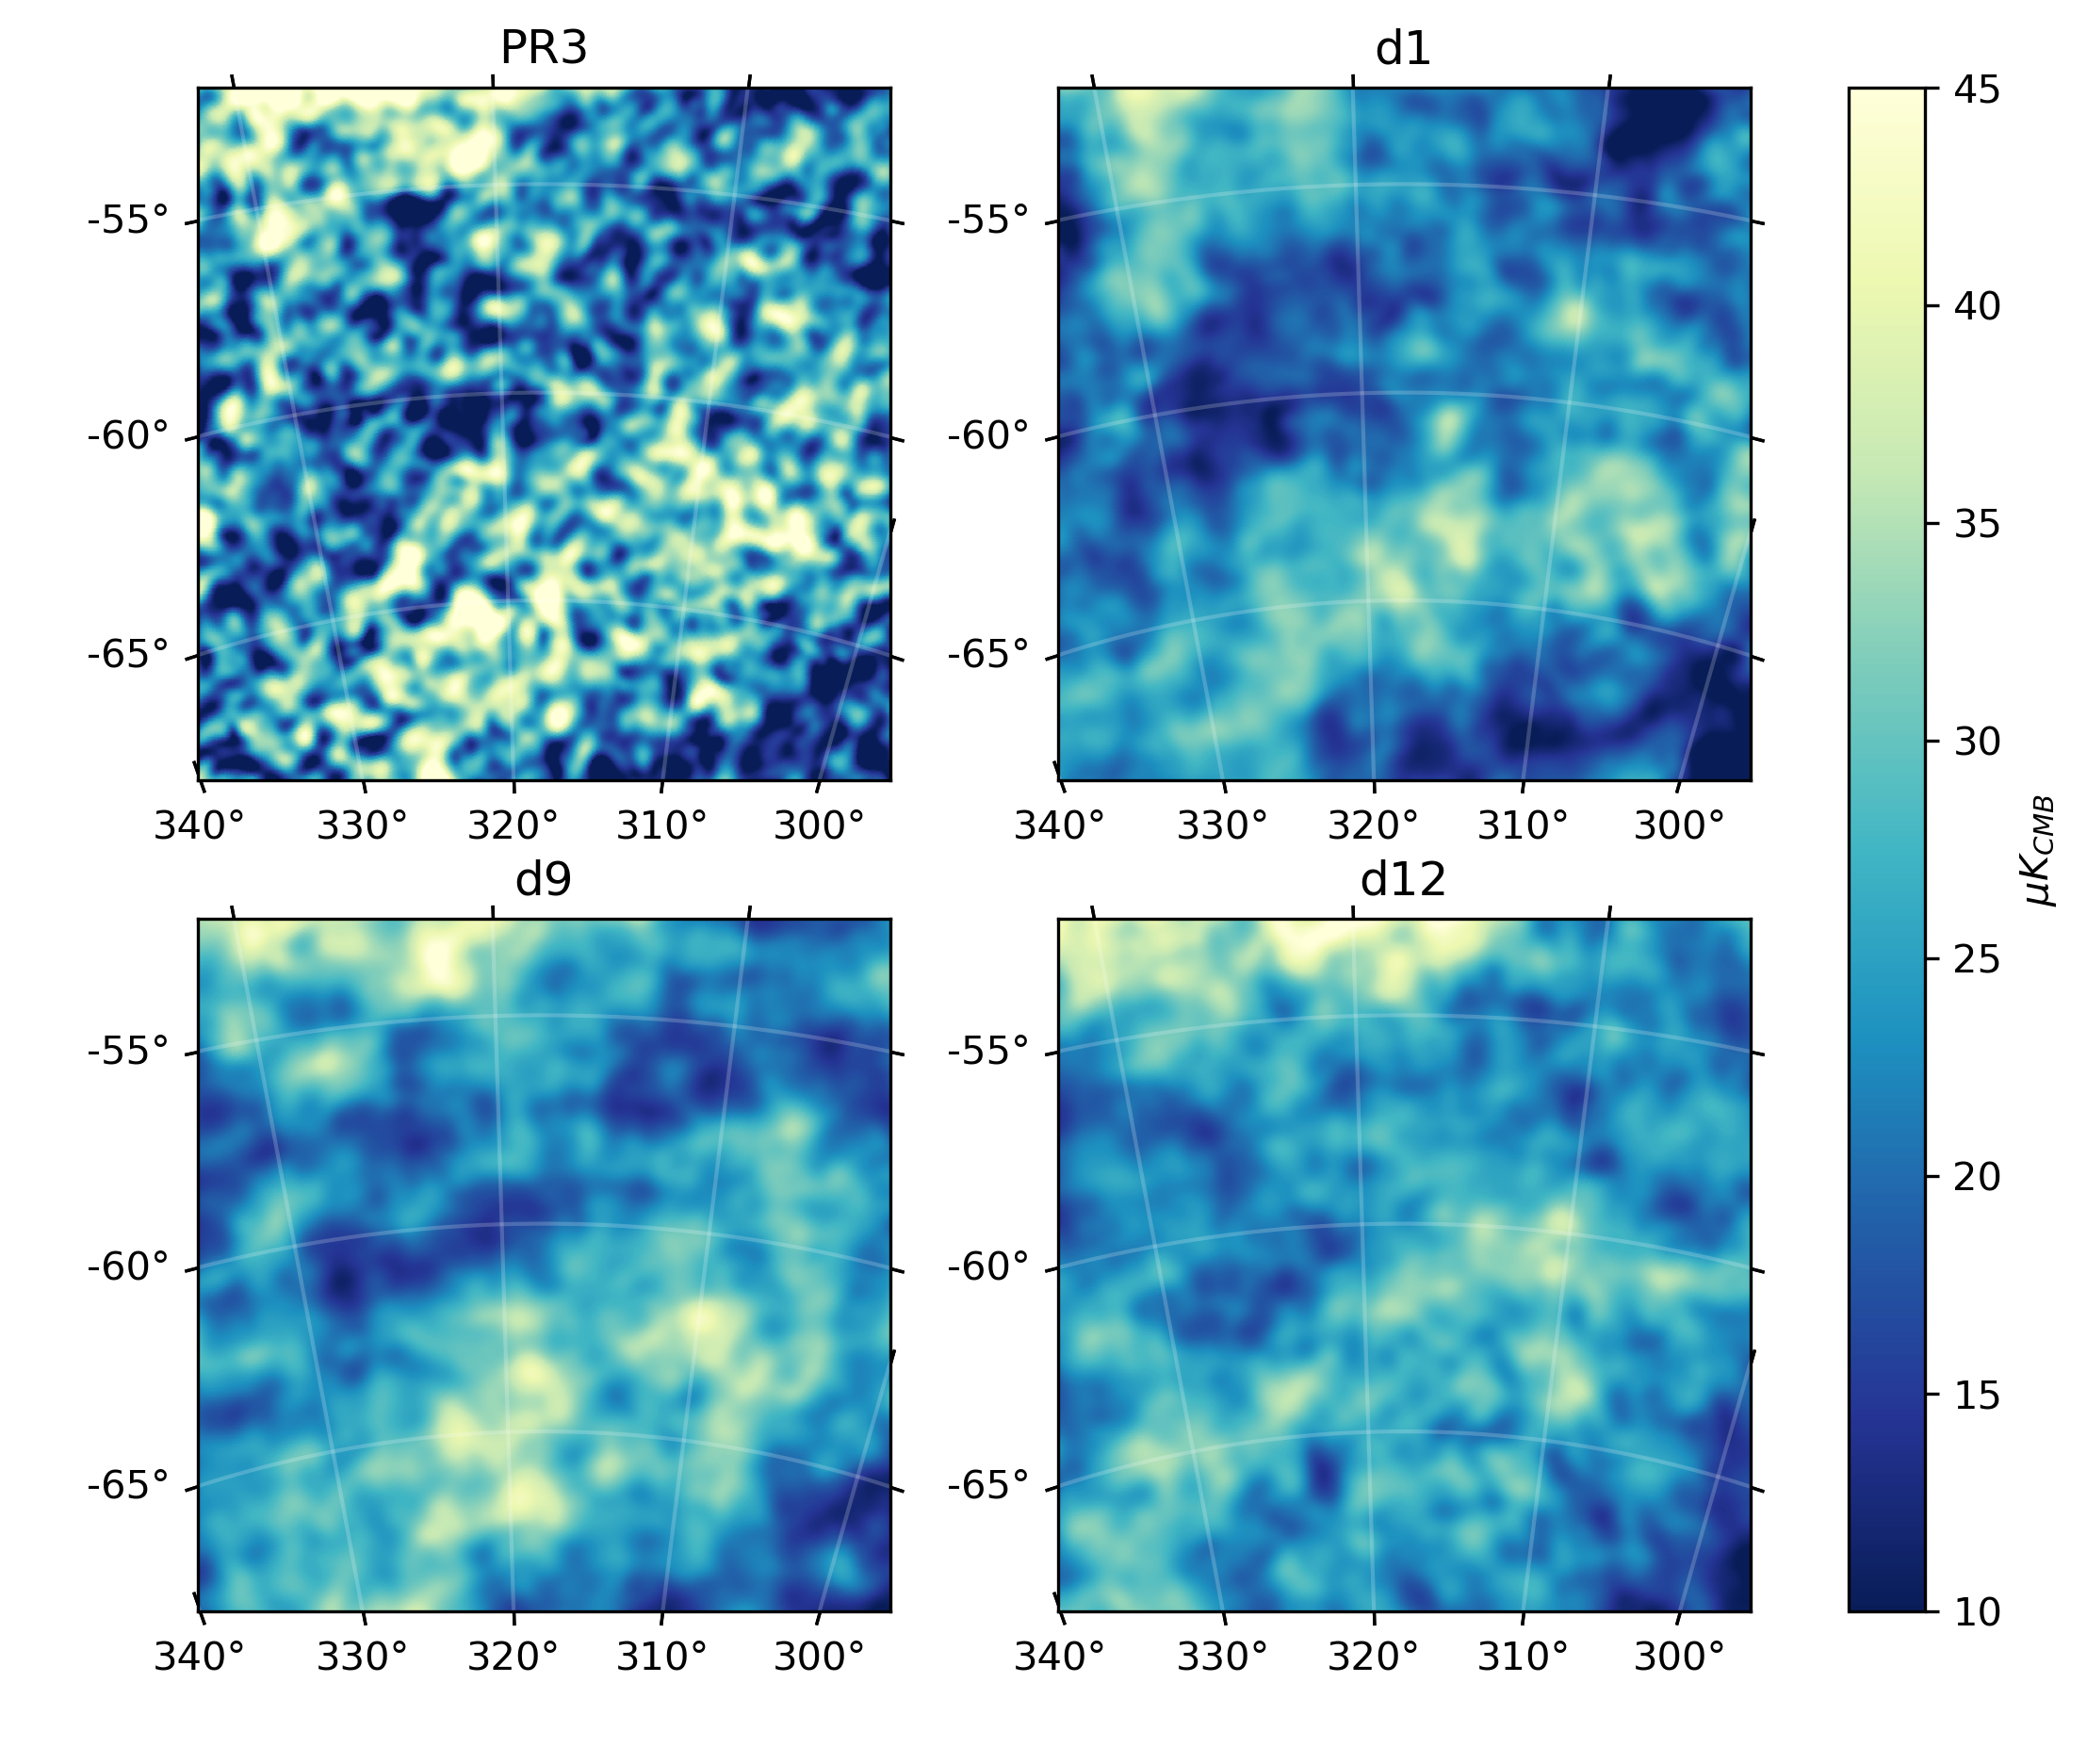
\includegraphics[width=0.48\textwidth]{figures/pol_BK_smooth_30'.png}
%     \caption{Polarized dust intensity at 353GHz centered at [l = 318, b = -61] with an angular resolution of 4.94', smoothed to 30 arcmin: (a) PR3 (b) d9 (c) d11 (d) d12.}
%     \label{fig:353_pol_int_BK}
% \end{figure}

% Intensity and polarization at 353~GHz are displayed in Figures~\ref{fig:353_int_gal_plane} to \ref{fig:353_pol_int_BK}. Varying choices for filtering the real data and generation of random small scales result in varying dust emission properties. For Intensity, d9 and d11 are very similar, with a loss of real structures, replaced by random realizations up to a scale of $l_{max} = 16384$, while d12 is more similar to the actual data. 
% Around the Bicep / Keck patch center (Figure~\ref{fig:353_int_BK}), the PR3 data is contaminated by the CIB, which masks out dust emission. 

% For the polarized intensity, close to the Galactic plane (Figure \ref{fig:353_pol_int_gal_plane}), we see a resemblance between the data and the three models. In the North and South poles, noise dominates in PR3 without smoothing, so the comparison is made at a resolution of $30\arcmin$. Overall, the agreement seems adequate between the models and the data considering the current level of uncertainties. 
% %After smoothing with a Gaussian beam of 30 arcmin, we discern dust structures.

% \subsection{Extragalactic Contamination} \label{sec:CIBcontamination}

% %[Stanford student Monica Hicks is working with Susan on cross-correlating our models with galaxy surveys a la Chiang \& Menard. Hopefully summary figure here.] 

% \begin{figure}[h!]
%     \centering
%     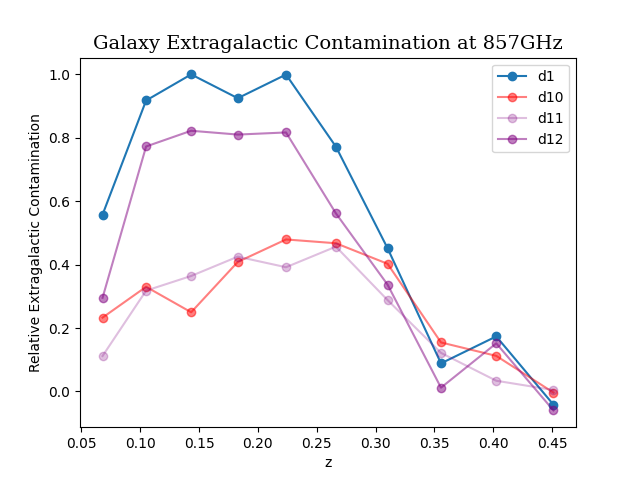
\includegraphics[width=\columnwidth]{figures/EGC_galaxy@857Part_0-1.png}
%     \caption{Relative extragalactic contamination in three of the new dust templates (\texttt{d10, d11, d12}), compared to the \texttt{d1} model. Contamination is quantified as the excess 857 GHz emission within $11'$ of galaxies from the GLADE+ catalog, normalized to the maximum excess and plotted as a function of redshift (z). All three new dust templates contain less extragalactic contamination than older dust models because they are based on GNILC-processed Planck data. The improvement is most significant for \texttt{d10} and \texttt{d11}.  }
%     \label{fig:extragal_contamination}
% \end{figure}


% %Our Galactic dust templates are based on measurements of the 
% We quantify the extragalactic contamination present in our dust models using a tomographic redshift-clustering technique \citep{Schmidt:2015, Chiang:2019}. Our intensity-based Galactic dust templates inevitably contain emission from both Galactic dust and external galaxies. As described in Section \ref{sec:dustamplitude}, the new \texttt{d9} and \texttt{d10} dust templates are derived from GNILC-processed Planck data, while older PySM dust templates used \texttt{Commander} data products. We thus expect that the new Galactic dust models are significantly less affected by CIB contamination than previous models. Here we quantify this contamination by measuring the angular cross-correlation between our dust models and the clustering of galaxies as a function of redshift in spectroscopic survey data. A perfect Galactic dust template would be uncorrelated with such clustering; the signature of CIB contamination is excess template emission correlated with galaxy clustering. 

% Following the procedure in \citet{Chiang:2019}, we compute the cross-correlation between local fluctuations in the Galactic emission maps and the galaxy density as a function of redshift, using galaxies from the GLADE+ catalog \citep{Dalya:2022}. We compute this cross-correlation for each of the \texttt{d1, d10, d11}, and \texttt{d12} dust emission templates at 857 GHz, at high Galactic latitudes ($\left|b\right| > 30\deg$). Figure \ref{fig:extragal_contamination} shows that while each of the new GNILC-based maps contain less extragalactic contamination than \texttt{d1}, the decreased contamination is more marked in \texttt{d10} and \texttt{d11} than in \texttt{d12}. This is likely due to [FILTERING CHOICES? TO DISCUSS WITH JACQUES]


\section{Future Outlook} \label{sec:discussion}

The Galactic emission models presented in this work are created from the latest data from large-area surveys like Planck, and informed by the latest literature constraints on the spectral behavior of Galactic emission components. These models incorporate some of the expected complexity of polarized emission at scales that are not yet well-constrained by data -- in particular, the non-Gaussianity of interstellar emission structure. While this represents a step forward in the realism of these models over previous all-sky Galactic emission models, there are a number of idealizations that could be improved in future work. 

The current models do not explicitly impose any non-zero parity-odd correlations in the polarized dust emission, i.e., the $TB$ and $EB$ correlations are zero in the power spectra that are used to extrapolate the small-scale dust emission structure. However, analysis of the Planck polarized dust emission finds a significant nonzero $TB$ correlation at $\ell \lesssim 600$ \citep{planck2016-l11A, Weiland:2020}. A proposed physical mechanism for the origin of the nonzero $TB$ signal is misalignment between dusty filaments and the projected magnetic field orientation \citep{Huffenberger:2020, Clark:2021, Cukierman:2023}: this picture also predicts the sign and amplitude of an expected nonzero $EB$ correlation. Future work could incorporate this parity-odd contribution to the polarized dust emission. Such models would be of particular use for the development of analysis techniques that seek to constrain signatures of cosmic birefringence or other parity-violating physics in the CMB \citep[e.g.,][]{Minami:2020, Eskilt:2022}.

Future work could also seek to improve the physical realism of the small-scale emission structure. The structure of polarized dust emission on small scales is highly filamentary \citep[e.g.,][]{Clark:2015, Halal:2024}. [TODO: say more]. Realizations of small-scale structure that have the particular character of non-Gaussianity that is realized in the sky could be generated using, for example, generative adversarial neural networks \citep{Krachmalnicoff:2021}.

In addition to the small-scale structure of the diffuse dust and synchrotron emission, the real sky at these frequencies contains emission from discrete sources that are not included in our models. These include cold clumps (cite Clancy), planetary nebulae ....

%\giuse{The models presented in this work represent a further step forward in order to increase the complexity of Galactic emission. They  exploit the latest templates from \emph{Planck } surveys as well as latest  constraints on the spectral parameters published in the literature in the past years. This is  critical in several CMB experiments as foreground complexity  could  potentially impact  the  cosmological parameter estimates. }

%\giuse{We carefully design new foreground  models to employ a non-zero level of non-gaussianity, allowing  unprecedented analysis and studies on non-gaussian small scales Galactic residuals and their impact on the de-lensing procedure of \emph{B-}modes. }


%\giuse{The algorithms presented here can be further improved as they  currently lack of parity odd correlations, e.g.  \emph{TB} and \emph{EB}. Although sensitivity from   current experiments have prevented to detect  correlations for both estimators letting alone  a positive $TB$  correlation  at large scales \citep{planck2016-l04}, there is increasing evidence of parity violating observations \citep{Eskilt:2022, Philcox:2022} indicating  the existence of  interactions with an exotic  particle related to the Cosmic birefringence mechanism. Moreover, physical mechanism of generating non-zero correlations of dust $EB$ and $TB$ spectra have been lately proposed in the literature related to the misalignement of dust filaments with the magnetic field lines CITE Clark/Huffenberger/Cukierman .} 

\section{Recommended Model Suite}\label{sec:modelsuite}

\begin{table*}
    \centering
    \begin{tabular}{p{0.1\textwidth} p{0.2\textwidth} p{0.5\textwidth}}
    
    \toprule 
    Complexity & Model set & Short description \\
    \midrule
    Low  & \texttt{d9, s4, f1, a1, co1} & Small-scale emission fluctuations in amplitude only; no frequency decorrelation in dust or synchrotron. Unpolarized CO emission.   \\
    Medium  & \texttt{d10, s5, f1, a1, co3} & Extrapolation to small scales for both amplitude and spectral parameters in dust and synchrotron. CO polarization at the 1\% level.  \\
    High  & \texttt{d12, s7, f1, a2, co3} & Dust layer model, spatially varying synchrotron curvature, polarized AME and CO.  \\
   
   \bottomrule
    \end{tabular}
    \caption{Summary of the suite of model sets described in Section \ref{sec:modelsuite}. These are recommended combinations of models at three levels of complexity (low, medium, and high).  }
    \label{tab:modelsuite}
\end{table*}

The models available for each emission component can be used in various combinations to form a number of unique Galactic sky models. While every user has this combinatoric freedom, we also prescribe a suite of recommended model sets. Our goal is to facilitate analyses that use a common set of assumptions. Community-wide use of this suite of Galactic emission model sets will enable easier comparisons between scientific forecasts for various experimental designs. This will also enable analyses that seek to explore synergies between multiple experiments -- for example, optimizing joint analyses of data from multiple telescopes. For example, these model sets can be used to explore the use of CMB-S4 high-resolution data to help delens LiteBIRD data, and LiteBIRD high-frequency data to help separate the dust foreground from CMB-S4 data. 

%for example analyzing CMB-S4 data together with that of the precursor South Pole and/or Simons Observatories, or using CMB-S4 high resolution data to help delens LiteBIRD and LiteBIRD high frequency data to help remove dust from CMB-S4.

Table~\ref{tab:modelsuite} details three model sets, representing increasing levels of complexity. The low complexity model set is highly idealized. Because this model implements small-scale synchrotron and dust fluctuations in amplitude alone, these components exhibit negligible frequency decorrelation (comparable to the \texttt{d1} model in Figure \ref{fig:decorrelation}).  
The medium complexity model set includes Galactic emission properties that are expected physically, %both expected physically and confirmed observationally, 
like sky-variable spectral parameters for the dust and synchrotron, extrapolated to small scales. 
The high complexity model set models Galactic emission properties that are physically realistic but as-yet undetected, like polarized AME and spatially varying synchrotron curvature. The high complexity model set uses the layer model for Galactic dust emission (Section~\ref{sec:layers}), and the decorrelation at frequencies dominated by the dust emission is near the maximum allowed by current constraints (Figure~\ref{fig:decorrelation}).

%[Moved from intro, work this in here:]
%for example analyzing CMB-S4 data together with that of the precursor South Pole and/or Simons Observatories, or using CMB-S4 high resolution data to help delens LiteBIRD and LiteBIRD high frequency data to help remove dust from CMB-S4.

\section{Summary and Conclusions} \label{sec:summary}

This work presents new models of Galactic emission, in total intensity and polarization, at frequencies relevant to CMB experiments. The models represent a data-driven understanding of the processes that dominate interstellar emission at these frequencies. We characterize various properties of the models in order to compare the models with each other and, where possible, validate them against observational constraints. We summarize the key conclusions of this work as follows:

\begin{enumerate}
    \item We develop new models of small-scale, non-Gaussian Galactic emission structure. We combine realizations of this small-scale synthetic emission with the latest component-separated Galactic emission data. We similarly extrapolate spectral parameters... The result is a set of all-sky models for   
    \item We demonstrate that the power spectra of our models broadly agree with data from Planck over large sky areas. 
    \item Summary of BK validation.
    \item We quantify the frequency decorrelation in our models by computing cross-power spectra. Our models span a range of decorrelation behavior, but we verify that all models are consistent with Planck constraints on decorrelation between 217 and 353 GHz. 
    
\end{enumerate}

Short forward-looking paragraph.

\begin{acknowledgments}

This work was supported by the National Science Foundation under grant No. AST-2106607 (PI S.E.C.). This work was carried out in part at the Jet Propulsion Laboratory, California Institute of Technology, under a contract with the National Aeronautics and Space Administration. We thank the BICEP/Keck collaboration for sharing the BK18 matrix products for the validation analysis of this paper. 

\end{acknowledgments}

\bibliography{refs.bib,refsADS.bib,refsPlanck.bib}

\end{document}